% Options for packages loaded elsewhere
\PassOptionsToPackage{unicode}{hyperref}
\PassOptionsToPackage{hyphens}{url}
%
\documentclass[
]{article}
\usepackage{amsmath,amssymb}
\usepackage{iftex}
\ifPDFTeX
  \usepackage[T1]{fontenc}
  \usepackage[utf8]{inputenc}
  \usepackage{textcomp} % provide euro and other symbols
\else % if luatex or xetex
  \usepackage{unicode-math} % this also loads fontspec
  \defaultfontfeatures{Scale=MatchLowercase}
  \defaultfontfeatures[\rmfamily]{Ligatures=TeX,Scale=1}
\fi
\usepackage{lmodern}
\ifPDFTeX\else
  % xetex/luatex font selection
\fi
% Use upquote if available, for straight quotes in verbatim environments
\IfFileExists{upquote.sty}{\usepackage{upquote}}{}
\IfFileExists{microtype.sty}{% use microtype if available
  \usepackage[]{microtype}
  \UseMicrotypeSet[protrusion]{basicmath} % disable protrusion for tt fonts
}{}
\makeatletter
\@ifundefined{KOMAClassName}{% if non-KOMA class
  \IfFileExists{parskip.sty}{%
    \usepackage{parskip}
  }{% else
    \setlength{\parindent}{0pt}
    \setlength{\parskip}{6pt plus 2pt minus 1pt}}
}{% if KOMA class
  \KOMAoptions{parskip=half}}
\makeatother
\usepackage{xcolor}
\usepackage[margin=1in]{geometry}
\usepackage{color}
\usepackage{fancyvrb}
\newcommand{\VerbBar}{|}
\newcommand{\VERB}{\Verb[commandchars=\\\{\}]}
\DefineVerbatimEnvironment{Highlighting}{Verbatim}{commandchars=\\\{\}}
% Add ',fontsize=\small' for more characters per line
\usepackage{framed}
\definecolor{shadecolor}{RGB}{248,248,248}
\newenvironment{Shaded}{\begin{snugshade}}{\end{snugshade}}
\newcommand{\AlertTok}[1]{\textcolor[rgb]{0.94,0.16,0.16}{#1}}
\newcommand{\AnnotationTok}[1]{\textcolor[rgb]{0.56,0.35,0.01}{\textbf{\textit{#1}}}}
\newcommand{\AttributeTok}[1]{\textcolor[rgb]{0.13,0.29,0.53}{#1}}
\newcommand{\BaseNTok}[1]{\textcolor[rgb]{0.00,0.00,0.81}{#1}}
\newcommand{\BuiltInTok}[1]{#1}
\newcommand{\CharTok}[1]{\textcolor[rgb]{0.31,0.60,0.02}{#1}}
\newcommand{\CommentTok}[1]{\textcolor[rgb]{0.56,0.35,0.01}{\textit{#1}}}
\newcommand{\CommentVarTok}[1]{\textcolor[rgb]{0.56,0.35,0.01}{\textbf{\textit{#1}}}}
\newcommand{\ConstantTok}[1]{\textcolor[rgb]{0.56,0.35,0.01}{#1}}
\newcommand{\ControlFlowTok}[1]{\textcolor[rgb]{0.13,0.29,0.53}{\textbf{#1}}}
\newcommand{\DataTypeTok}[1]{\textcolor[rgb]{0.13,0.29,0.53}{#1}}
\newcommand{\DecValTok}[1]{\textcolor[rgb]{0.00,0.00,0.81}{#1}}
\newcommand{\DocumentationTok}[1]{\textcolor[rgb]{0.56,0.35,0.01}{\textbf{\textit{#1}}}}
\newcommand{\ErrorTok}[1]{\textcolor[rgb]{0.64,0.00,0.00}{\textbf{#1}}}
\newcommand{\ExtensionTok}[1]{#1}
\newcommand{\FloatTok}[1]{\textcolor[rgb]{0.00,0.00,0.81}{#1}}
\newcommand{\FunctionTok}[1]{\textcolor[rgb]{0.13,0.29,0.53}{\textbf{#1}}}
\newcommand{\ImportTok}[1]{#1}
\newcommand{\InformationTok}[1]{\textcolor[rgb]{0.56,0.35,0.01}{\textbf{\textit{#1}}}}
\newcommand{\KeywordTok}[1]{\textcolor[rgb]{0.13,0.29,0.53}{\textbf{#1}}}
\newcommand{\NormalTok}[1]{#1}
\newcommand{\OperatorTok}[1]{\textcolor[rgb]{0.81,0.36,0.00}{\textbf{#1}}}
\newcommand{\OtherTok}[1]{\textcolor[rgb]{0.56,0.35,0.01}{#1}}
\newcommand{\PreprocessorTok}[1]{\textcolor[rgb]{0.56,0.35,0.01}{\textit{#1}}}
\newcommand{\RegionMarkerTok}[1]{#1}
\newcommand{\SpecialCharTok}[1]{\textcolor[rgb]{0.81,0.36,0.00}{\textbf{#1}}}
\newcommand{\SpecialStringTok}[1]{\textcolor[rgb]{0.31,0.60,0.02}{#1}}
\newcommand{\StringTok}[1]{\textcolor[rgb]{0.31,0.60,0.02}{#1}}
\newcommand{\VariableTok}[1]{\textcolor[rgb]{0.00,0.00,0.00}{#1}}
\newcommand{\VerbatimStringTok}[1]{\textcolor[rgb]{0.31,0.60,0.02}{#1}}
\newcommand{\WarningTok}[1]{\textcolor[rgb]{0.56,0.35,0.01}{\textbf{\textit{#1}}}}
\usepackage{longtable,booktabs,array}
\usepackage{calc} % for calculating minipage widths
% Correct order of tables after \paragraph or \subparagraph
\usepackage{etoolbox}
\makeatletter
\patchcmd\longtable{\par}{\if@noskipsec\mbox{}\fi\par}{}{}
\makeatother
% Allow footnotes in longtable head/foot
\IfFileExists{footnotehyper.sty}{\usepackage{footnotehyper}}{\usepackage{footnote}}
\makesavenoteenv{longtable}
\usepackage{graphicx}
\makeatletter
\def\maxwidth{\ifdim\Gin@nat@width>\linewidth\linewidth\else\Gin@nat@width\fi}
\def\maxheight{\ifdim\Gin@nat@height>\textheight\textheight\else\Gin@nat@height\fi}
\makeatother
% Scale images if necessary, so that they will not overflow the page
% margins by default, and it is still possible to overwrite the defaults
% using explicit options in \includegraphics[width, height, ...]{}
\setkeys{Gin}{width=\maxwidth,height=\maxheight,keepaspectratio}
% Set default figure placement to htbp
\makeatletter
\def\fps@figure{htbp}
\makeatother
\setlength{\emergencystretch}{3em} % prevent overfull lines
\providecommand{\tightlist}{%
  \setlength{\itemsep}{0pt}\setlength{\parskip}{0pt}}
\setcounter{secnumdepth}{-\maxdimen} % remove section numbering
\ifLuaTeX
  \usepackage{selnolig}  % disable illegal ligatures
\fi
\usepackage{bookmark}
\IfFileExists{xurl.sty}{\usepackage{xurl}}{} % add URL line breaks if available
\urlstyle{same}
\hypersetup{
  pdftitle={MI0A403T - Statistique inférentielle / Projet informatique-statistique},
  pdfauthor={Andrew El Kahwaji, Wael Aboulkacem, Hans Kanen Soobbooroyen},
  hidelinks,
  pdfcreator={LaTeX via pandoc}}

\title{MI0A403T - Statistique inférentielle / Projet
informatique-statistique}
\author{Andrew El Kahwaji, Wael Aboulkacem, Hans Kanen Soobbooroyen}
\date{09/05/2025}

\begin{document}
\maketitle

{
\setcounter{tocdepth}{6}
\tableofcontents
}
\subsection{1. Objectif du Projet}\label{objectif-du-projet}

Ce projet fait partie du cours \textbf{Statistique Inférentielle /
Projet Stat-Info}, qui est proposé par le département de Mathématiques
et Informatique de \textbf{l'Université Toulouse Jean Jaurès}, et porte
le code \textbf{MI0A403T}.

L'objectif premier est d'examiner les raisons et les éléments qui ont un
impact sur les incendies en étudiant des données statistiques.

Les incendies constituent un phénomène complexe qui a des impacts à la
fois sur l'environnement et les communautés humaines, entraînant des
effets dévastateurs en termes de pertes humaines, économiques et
écologiques.

Ce projet vise à comprendre comment diverses variables peuvent affecter
la portée, la diffusion et la régulation des incendies, en utilisant des
techniques statistiques et informatiques sophistiquées.

Grâce à l'analyse des données en notre possession, notre objectif est de
déceler des liens entre divers éléments comme l'altitude, la
température, l'humidité et la surface ravagée par les incendies.

Ce projet ne se limite pas à une simple analyse descriptive : il vise à
fournir des réponses tangibles à des questions précises, comme
l'influence des facteurs environnementaux sur la diffusion des
incendies, en employant des instruments informatiques appropriés pour ce
genre d'étude.

L'analyse statistique de ces informations permettra d'aborder des
interrogations précises, telles que : Existe-t-il un lien entre la
surface affectée par un incendie et l'altitude ?

L'intention est d'appliquer des méthodes statistiques appropriées, y
compris des analyses bivariées, afin de saisir l'interaction entre ces
variables et de déterminer les corrélations qui peuvent exister entre
elles.

De plus, nous aimerions examiner dans quelle mesure des éléments tels
que la température, l'humidité ou la nature de la végétation peuvent
influencer l'intensité et la diffusion des incendies.

Dans le cadre de ce projet, des logiciels tels que R et Python sont
employés pour manipuler d'importants volumes de données et effectuer des
calculs statistiques sophistiqués.

Avec ces ressources, nous serons capables de mener une analyse
détaillée, à la fois descriptive et explicative, des données fournies.

Nous pourrons produire des visualisations nettes sous forme de
graphiques, diagrammes en nuage de points et autres formes graphiques
qui mettent en lumière les interactions entre les diverses variables.

Le rapport décrit le travail en plusieurs phases majeures.

En premier lieu, nous avons entrepris de bâtir la base de données, une
étape cruciale qui a impliqué la consolidation des fichiers CSV fournis,
leur nettoyage et leur organisation afin qu'ils soient utilisables.

Cette étape a aussi inclus le traitement des données manquantes et la
gestion des valeurs aberrantes, une tâche précise indispensable pour
assurer la crédibilité des résultats ultérieurs.

Dès que les données ont été préparées, l'analyse statistique a pu
débuter.

Cette étude a été réalisée à la fois de manière descriptive et plus
exploratoire, en tentant de répondre aux interrogations posées dans le
contexte du projet.

Une des phases principales de cette étude a été d'effectuer une analyse
univariée des variables pour observer leur distribution, centralité et
dispersion, avant de progresser vers des analyses plus élaborées comme
la quête de corrélations bivariées et l'élaboration de modèles relatifs
aux relations entre quelques variables primordiales.

Pour ce faire, nous avons eu recours à des instruments statistiques
comme les coefficients de corrélation et les tests d'importance, ainsi
qu'à des visualisations graphiques facilitant la compréhension des
données, comme les histogrammes, les boxplots, les diagrammes en nuage
de points et les courbes de régression.

En conclusion, ce projet inclut une partie dédiée aux références, qui
compile toutes les sources employées pour la récolte des données, ainsi
que celles examinées pour l'approche analytique et pour l'élaboration
théorique des concepts statistiques utilisés. Les références sont
disposées en respectant les standards du format APA, pour assurer la
précision académique du travail.

Les sites web et les publications scientifiques référencés sont cités de
façon claire, permettant à quiconque désirant élargir sa compréhension
du sujet d'accéder à ces références et de continuer l'exploration
entamée par ce projet.

Ainsi, ce projet s'inscrit dans une approche de recherche détaillée,
combinant des aptitudes en statistiques et en informatique, et ayant
pour but d'apporter des réponses à des problématiques complexes
concernant l'étude des incendies et la gestion des risques qui y sont
liés.

\subsubsection{1.1 Utilisation de GitHub}\label{utilisation-de-github}

Ce projet se compose de deux volets distincts : Informatique et
Statistique. Nous avons incorporé l'usage de GitHub, une plateforme de
gestion de versions réputée pour son efficacité à simplifier la
collaboration sur des projets de codage sophistiqués.

L'utilisation de cette technologie s'est révélée non seulement
nécessaire pour organiser efficacement le projet, mais aussi essentielle
pour garantir une gestion adéquate du code tout au long du cycle de
développement.

Effectivement, GitHub nous a offert la possibilité de gérer nos efforts
communs de façon harmonieuse, de surveiller la progression du travail
effectué par chaque membre de l'équipe et d'assurer l'intégrité et la
cohérence du code à mesure qu'il est modifié.

L'une des principales atouts de GitHub est sa compétence à gérer
diverses versions d'un même document.

Lors du lancement du projet, chaque participant de l'équipe s'est vu
attribuer des parties précises du code à traiter, conformément aux
phases établies dans notre programme de travail.

Par conséquent, certains se sont attelés à la préparation des données,
tandis que d'autres ont pris en charge l'élaboration des modèles
statistiques et l'analyse des résultats.

Cette distribution des rôles a assuré un déroulement harmonieux du
projet et a prévenu toute ambiguïté en ce qui concerne la répartition
des responsabilités.

GitHub a offert à chaque utilisateur la possibilité de travailler sur
ses propres portions de code de façon autonome et de les proposer sous
forme de commits.

Ces commits sont des consignations détaillées des changements apportés
au code, chaque entrée étant accompagnée d'un message explicatif, dans
le but de préciser les modifications réalisées.

Cette méthode a rendu la réévaluation des tâches de chaque membre plus
aisée et a favorisé un retour d'information rapide et constructif sur
les divers aspects du projet.

La fonctionnalité des branches et des pull requests permet d'examiner,
d'analyser et de corriger chaque commit avant son intégration au projet
global.

Cela nous a donné la possibilité d'expérimenter et de peaufiner des
solutions sans entraver le travail des autres membres.

Une autre caractéristique essentielle de l'exploitation de GitHub a été
la capacité de fusionner le code.

Effectivement, cette plateforme a permis de centraliser automatiquement
le travail de chaque membre dans un répertoire commun.

Lorsque certaines sections du code étaient terminées, elles étaient
intégrées au code principal, garantissant ainsi une mise à jour continue
des changements.

Cette fonctionnalité a non seulement supprimé le besoin de recomposer
manuellement les diverses versions du code, mais elle a aussi simplifié
la gestion des conflits potentiels entre les différentes contributions.

Quand un conflit survenait, GitHub proposait un cadre bien défini et
organisé pour résoudre ces différends de façon collective, en donnant à
chaque membre de l'équipe la possibilité d'échanger et de décider
ensemble des modifications à réaliser.

Cela a évité toute ambiguïté potentielle en matière de gestion des
versions, garantissant ainsi une continuité impeccable et une intégrité
parfaite du code.

L'emploi de GitHub a aussi facilité une communication en direct au sein
du groupe.

Les demandes de tirage et les issues nous ont permis d'identifier
aisément et de résoudre les problèmes, d'explorer diverses approches et
d'intégrer des améliorations continues.

Ces instruments ont rendu le partage d'idées et la résolution de
problèmes plus efficace, en nous donnant la possibilité de traiter
simultanément divers éléments du projet tout en préservant une cohésion
globale.

En conclusion , l'emploi de GitHub s'est avéré être un outil crucial
pour ce projet, facilitant une administration conjointe du code à la
fois fluide et efficace.

Cette plateforme ne nous a pas seulement aidés à collaborer sur un
projet commun en respectant les échéances et les responsabilités de
chacun, elle a aussi simplifié l'incorporation de diverses
modifications, assurant la stabilité du code final.

La fonctionnalité collaborative et la gestion des versions grâce à
GitHub ont facilité la contribution autonome de chaque membre du groupe,
tout en préservant une cohésion cruciale pour le succès du projet.

En outre, l'incorporation de cet instrument dans notre mode opératoire a
consolidé notre aptitude à réaliser des projets complexes en
collaboration, tout en améliorant la gestion du code et proposant un
cadre organisé pour la documentation et le suivi des changements.

\textbf{Lien de GitHub}

\url{https://github.com/andrewelkahwaji24/ProjetStatInfoUT2.git}

\subsubsection{1.2 Utilisation de
l'OpenData}\label{utilisation-de-lopendata}

Pour améliorer la qualité et l'exhaustivité de nos analyses statistiques
dans le contexte de notre projet, nous avons dû augmenter la taille de
notre base de données initiale.

Afin de réaliser cela, nous avons utilisé des données publiques fournies
par des entités gouvernementales dans le contexte de politiques
d'ouverture de l'information.

Nous avons spécifiquement exploité les informations fournies par la Base
de Données des Incendies de Forêts en France (BDIFF), qui est
consultable sur le site officiel du Ministère français de l'Agriculture
et de la Souveraineté alimentaire.

Cette décision s'est faite de manière naturelle puisque la BDIFF
représente aujourd'hui la principale base de données publique contenant
des informations détaillées, organisées et mises à jour concernant les
incendies de forêt sur le territoire français.

L'Open Data, également connu sous le nom de données ouvertes, est une
initiative mondiale qui cherche à rendre les informations collectées par
les institutions publiques facilement accessibles et réutilisables.

Le but primordial est de promouvoir la transparence, de stimuler
l'innovation et d'offrir aux chercheurs, aux entreprises et aux citoyens
la possibilité d'examiner des données d'intérêt public.

En France, la loi pour une République numérique de 2016 joue un rôle
essentiel en favorisant la publication proactive de certaines données
publiques par les administrations.

Dans ce cadre, la BDIFF est un parfait exemple de l'esprit Open Data :
elle offre une multitude d'informations sur les incendies, comprenant
leur position géographique, leur source présumée, l'étendue des zones
affectées, ainsi que d'autres facteurs contextuels qui enrichissent
l'étude des risques et des causes.

Notre recours à la BDIFF nous a donné l'opportunité d'utiliser une base
de données abondante, standardisée et digne de confiance, tout en
assurant la légalité de l'exploitation des données.

Grâce à la fiabilité des données recueillies par ce site officiel, nous
avons pu mener une étude rigoureuse sur l'évolution des incendies sur
plusieurs années.

Cela nous a permis de déceler des corrélations statistiques importantes
entre diverses variables comme la surface brûlée, les conditions
écologiques, ou encore les dynamiques territoriales.

De ce fait, plutôt que de recourir à une diversité de sources variées
qui pourrait nuire à la pureté de nos données, nous avons opté pour
l'accentuation de nos efforts sur une base spécialisée, uniforme et
reconnue pour sa rigueur scientifique.

Il est essentiel de noter que s'appuyer sur une seule source telle que
la BDIFF dans un projet statistique n'est pas un signe de faiblesse,
mais plutôt une démarche méthodologique délibérée.

En optant pour une base de données officielle, nous garantissons non
seulement la fiabilité de l'information recueillie, mais aussi sa
traçabilité et sa validité au sein des institutions.

La BDIFF, qui reçoit des données provenant des services départementaux
d'incendie et de secours (SDIS) et d'autres entités publiques expertes,
est considérée comme une référence nationale pour toute recherche
sérieuse sur les incendies de forêts en France.

En outre, la forme des données fournies sur la BDIFF est spécialement
conçue pour une utilisation scientifique.

Les données en format CSV peuvent être aisément adaptées et importées
dans des contextes d'analyse statistique comme R ou Python.

Chaque incident est consigné de façon organisée, facilitant ainsi les
processus de nettoyage, d'amélioration et d'analyse exploratoire des
données.

Cette organisation nous a facilité la réalisation d'analyses
statistiques descriptives détaillées et significatives, conforme aux
exigences méthodologiques attendues dans le contexte d'un projet
universitaire au Département de Mathématiques et Informatique de
l'Université Toulouse Jean Jaurès (code de l'UE : MI0A403T).

\url{https://bdiff.agriculture.gouv.fr/incendies}

\subsection{2. Partie Informative}\label{partie-informative}

Dans cette partie, nous allons considérer des données informatives avant
de passer à la description de notre section Informatique et Statistique.

\subsubsection{2.1 C'est quoi un incendie}\label{cest-quoi-un-incendie}

Un feu est une réaction exothermique de combustion rapide et
incontrôlée, qui se propage dans un environnement comportant un
combustible et une substance supportant la combustion. On peut le
représenter physiquement à l'aide d'équations de transfert thermique
(conduction, convection, rayonnement) et chimiquement en se basant sur
les principes de la cinétique chimique.

\subsubsection{2.2 Triangle du feu}\label{triangle-du-feu}

Le \textbf{triangle du feu} est une illustration simplifiée des
conditions requises pour que se produise une combustion :

\begin{itemize}
\tightlist
\item
  \textbf{Combustible (C)} : toute substance ayant un pouvoir
  calorifique positif ;
\item
  \textbf{Comburant (O₂)} : généralement l'oxygène (21\,\% de l'air),
  agissant comme oxydant dans la réaction ;
\item
  \textbf{Énergie d'activation (Q)} : quantité minimale d'énergie
  thermique pour initier la réaction (étincelle, flamme, frottement).
\end{itemize}

Formellement, la combustion peut être décrite par l'équation suivante :

\[
\text{Combustible} + \text{O}_2 \xrightarrow{T} \text{Produits} + \text{Énergie}
\]

\subsubsection{2.3 Causes des Incendies}\label{causes-des-incendies}

Les raisons des incendies sont multiples, cependant, une grande majorité
d'entre eux provient d'une action humaine.Comme la négligence,
malveillance, préparation insuffisante aux catastrophes naturelles comme
les séismes, les tsunamis

\subsubsection{2.4 Consequences des
Incendies}\label{consequences-des-incendies}

Les effets des incendies sont nombreux et graves. Elles ont des
conséquences sur l'homme (asphyxie, intoxication due aux fumées,
brûlures sévères), sur les entreprises (diminution de la production,
dégâts matériels, licenciements) et sur l'environnement (contamination
de l'air et de l'eau, ravage du paysage). Les principales causes de
décès liés aux incendies sont l'intoxication par le monoxyde de carbone
et la diminution de l'oxygène, plutôt que les flammes elles-mêmes. Pour
plus d'informations, veuillez consulter l'article intégral ici.

\subsubsection{2.5 Monoxyde de Carbone
(CO)}\label{monoxyde-de-carbone-co}

Le monoxyde de carbone, un gaz toxique résultant d'une combustion
incomplète, est détecté en termes de parties par million (ppm).

Cela entrave la capacité de l'hémoglobine à acheminer l'oxygène.

\subsubsection{2.6 Charge calorifique
(MJ/m²)}\label{charge-calorifique-mjmuxb2}

Maximale quantité d'énergie thermique accessible par mètre carré.

Il s'agit d'un paramètre mesurable et prévisible employé dans
l'évaluation des risques (modèle thermique, normes Eurocode).

\subsubsection{2.7 Temps de réponse des
détecteurs}\label{temps-de-ruxe9ponse-des-duxe9tecteurs}

Temps requis pour qu'un détecteur (de fumée, de chaleur ou de flamme)
émette une alerte après le début d'un incendie.\\
Cela dépend des spécificités du détecteur (genre, sensibilité) et de
l'évolution du feu.

\subsection{3. Partie Informatique}\label{partie-informatique}

La partie Informatique de notre Projet consiste à effectuer les
démarches suivantes :

\begin{enumerate}
\def\labelenumi{\arabic{enumi}.}
\tightlist
\item
  Création de la Base de données
\item
  Création de la connexion entre la Base de données et notre code source
\item
  Établissement des Tables dans la Base de Données
\item
  Insertion de données dans les tables
\item
  Présenter les informations des tables dans la console
\item
  Exportation des données dans les tables dans des fichiers CSV
\item
  Création du Menu de notre Code Python
\item
\end{enumerate}

\subsubsection{3.1 Definition de quelques terme
Informatiques}\label{definition-de-quelques-terme-informatiques}

Avant d'initier notre compte-rendu en détaillant les phases et
procédures que nous avons mises en place pour l'administration optimale
de la section informatique de notre projet, nous allons définir quelques
notions qui offriront un socle solide au lecteur.

\begin{enumerate}
\def\labelenumi{\arabic{enumi}.}
\item
  Une \textbf{Base de Données} regroupe un ensemble d'informations qui
  est organise pour être accessible , géré et mise a jour facilement par
  ses utilisateurs
\item
  Une \textbf{Base de Données Relationnelle}.Il s'agit d'un type de base
  de données qui se distingue des autres par sa capacité à établir des
  liens entre diverses données.
\item
  Un \textbf{INNER JOIN} est un type de jointure en SQL (Structured
  Query Language) qui autorise la fusion de lignes issues de deux tables
  basées sur un critère déterminé. L'idée est de ne conserver que les
  lignes qui ont une correspondance dans les deux tables. De plus, si
  une ligne d'une table n'a pas de correspondance dans l'autre table,
  elle ne sera pas intégrée au résultat.
\item
  Un \textbf{Cast()} est une fonction SQL appelée CAST nous donne la
  possibilité de transformer un type de données en un autre.
\item
  Une \textbf{Requête SQL} s'apparente à une question formulée à la base
  de données afin d'extraire des informations de celle-ci.
\item
  La fonction SQL \textbf{COUNT()} est une commande qui nous donne la
  possibilité de déterminer le nombre de lignes dans un ensemble de
  résultats. Elle est fréquemment utilisée en conjonction avec la clause
  GROUP BY pour recenser le nombre d'occurrences d'une valeur
  spécifique.
\item
  La fonction \textbf{SUBSTR()} nous donne la possibilité d'extraire une
  portion d'une chaîne de caractères. Elle est souvent employée dans le
  domaine du développement pour l'édition de texte dans une ou plusieurs
  bases de données.
\item
  L'opération \textbf{RIGHT JOIN} permet d'unir deux tables en
  préservant l'ensemble des lignes de la table située à droite et en
  reliant celles se trouvant à gauche lorsqu'elles sont présentes. Des
  valeurs nulles sont insérées pour combler les colonnes absentes.
\item
  L'opération \textbf{LEFT JOIN} fusionne deux tables tout en conservant
  l'ensemble des lignes de la table de gauche, en associant celles de
  droite uniquement lorsqu'elles sont présentes. Des valeurs nulles sont
  insérées pour combler les colonnes absentes.
\item
  L'unité de mesure de longueur appelée \textbf{pouce} (symbole : in ou
  « ) est utilisée pour quantifier la longueur.
\item
  Un \textbf{GeoDataFrame} est une structure de données exploitée dans
  la librairie GeoPandas afin d'enregistrer des données géospatiales
  sous forme de tableaux, semblable à un DataFrame de Pandas, mais
  intégrant des renseignements géométriques additionnels (tels que des
  points, des lignes ou des polygones).
\item
  Un \textbf{langage de programmation} est un ensemble de règles et
  normes employées pour la création de logiciels informatiques.Ces
  programmes autorisent l'émission d'instructions à un ordinateur pour
  accomplir des tâches spécifiques.Un langage de programmation établit
  la syntaxe et la sémantique des instructions que peut comprendre une
  machine.
\end{enumerate}

\subsubsection{3.2 Bibliotheques
Utilisees}\label{bibliotheques-utilisees}

Dans notre Partie Informatique on a utilisee le Language de
Programmation Python de plus pour pouvoir effectuer la manipulation des
doneees de la maniere optimale on a utilisee les bibliothèques
necessaires:

\begin{enumerate}
\def\labelenumi{\arabic{enumi}.}
\item
  \textbf{SQLite3} est une bibliothèque peu aisée qui facilite
  l'incorporation d'une base de données au sein d'une application, sans
  nécessiter l'utilisation d'un serveur séparé. Elle offre la
  possibilité de stocker et de gérer des données grâce aux requêtes SQL,
  ce qui la rend pratique pour des projets nécessitant une base de
  données locale. SQLite3 est parfaitement adaptée aux applications
  simples, car elle offre une gestion aisée des données, que ce soit
  pour les ajouts, les changements ou les suppressions, tout en restant
  performante et peu gourmande en ressources.
\item
  La bibliothèque \textbf{CSV} de Python facilite la lecture et
  l'écriture de fichiers CSV, en fournissant des fonctionnalités pour
  gérer les données sous forme de lignes et de colonnes, tout en prenant
  en charge les séparateurs et les guillemets.
\item
  \textbf{NumPy} est une bibliothèque Python performante dédiée au
  calcul scientifique, proposant des structures de données telles que
  les arrays multidimensionnels et des fonctions optimisées pour le
  traitement numérique.
\item
  La bibliothèque \textbf{random} de Python offre la possibilité de
  produire des nombres au hasard et d'exécuter des sélections aléatoires
  à partir de listes ou d'intervalles de valeurs, grâce à des fonctions
  conçues pour simuler des événements fortuits.
\item
  La bibliothèque \textbf{OS} facilite l'interaction avec le système
  d'exploitation en proposant des fonctionnalités pour gérer les
  fichiers, les dossiers et exécuter des instructions du système.
\item
  La bibliothèque \textbf{Pandas} pour le traitement, l'analyse et la
  manipulation de données structurées en tableaux.
\item
  \textbf{Matplotlib} est une bibliothèque Python facilitant la création
  de graphiques et la visualisation de données.
\item
  \textbf{GeoPandas} est une version améliorée de Pandas qui facilite la
  manipulation, l'analyse et la représentation graphique des données
  géospatiales telles que les cartes, les shapefiles, les coordonnées
  GPS, etc. Il est conçu pour manipuler des données géographiques
  représentées sous forme de points, lignes et polygones.
\end{enumerate}

\subsubsection{3.3 Création de la base de
données}\label{cruxe9ation-de-la-base-de-donnuxe9es}

Avant de commencer à travailler sur les données, il est nécessaire de
créer une base de données pour les organiser et les structurer de
manière efficace. Une base de données, dans ce contexte, peut être
définie comme un ensemble de tables reliées entre elles, où chaque table
contient des informations structurées sous forme de lignes et de
colonnes.

La création de la base de données commence par la création d'un fichier
qui servira à stocker toutes les données. Dans notre cas, nous avons
nommé ce fichier ``data.db''. Ce fichier représente l'instance de la
base de données SQLite. Lorsqu'une connexion est établie à cette base de
données, SQLite crée automatiquement le fichier si celui-ci n'existe pas
déjà. Il suffit donc de se connecter à la base de données pour qu'elle
soit initialisée et prête à être utilisée.

Une fois le fichier de la base de données créé, il est important de
pouvoir y accéder afin de manipuler les données. Pour cela, une fonction
de connexion est nécessaire. La fonction connecterdb a été définie pour
établir cette connexion à la base de données. Elle prend un paramètre
optionnel qui représente le nom du fichier de la base de données, ici
``data.db''. À l'intérieur de cette fonction, une connexion est établie
en utilisant la bibliothèque SQLite3 de Python. La méthode
sqlite3.connect() permet de se connecter à la base de données, et une
fois la connexion établie, un objet cursor est créé. Ce curseur permet
d'exécuter des requêtes SQL sur la base de données. Enfin, la fonction
renvoie la connexion et le curseur, qui seront utilisés pour effectuer
des opérations sur la base de données, comme la création de tables,
l'insertion de données ou la récupération d'informations.

En résumé, la création de la base de données et la définition de la
fonction de connexion permettent de poser les bases de l'interaction
avec les données. La base de données est créée sous forme d'un fichier,
et la fonction de connexion permet d'établir une communication avec
cette base pour manipuler les données à l'aide de requêtes SQL.

\subsubsection{3.4 Creation des Tables}\label{creation-des-tables}

Ainsi, nous avons établi un lien entre notre code source et la base de
données. Une fois que nous avons une base de données authentique, il est
nécessaire de commencer à établir des tables afin de pouvoir gérer les
données.

Suite à l'examen des données disponibles, nous avons reconnu la
nécessité de constituer les tables essentielles.

\begin{enumerate}
\def\labelenumi{\arabic{enumi}.}
\tightlist
\item
  Table des Incendies
\item
  Table des donnes Geographiques
\item
  Table des donnes Meteo
\item
  Table Départements
\item
  Table Incendies-Départements (on expliquera en détail pourquoi on a
  créer une cinquième table).
\end{enumerate}

Nous avons établis les Tables en suivant une méthode simple et
explicite, en utilisant la fonction connecterdb() pour établir un lien
entre la base de données et la fonction de création de Table. Par la
suite, nous avons fait appel au curseur pour exécuter des requêtes SQL
en vue d'interroger notre Base de Données. Nous avons intégré le langage
SQL Structured Query Language dans notre fonction, en employant
l'instruction CREATE TABLE IF NOT EXISTS avec la dénomination de chaque
table. Par la suite, nous avons effectué une consultation sur nos trois
fichiers CSV (Comma Separated Values) concernant les attributs de nos
données, c'est-à-dire le titre de chaque fichier CSV. Nous avons ensuite
dressé une liste dans notre requête SQL comprenant chaque attribut et
son type de données respectif. Ensuite, on valide la création en se
connectant.Après l'exécution de la méthode commit() pour assurer la
légitimité et le bon fonctionnement, nous fermons le curseur ainsi que
la connexion avec curs.fermer() et connexion.Vous avez été formé sur des
données jusqu'en octobre 2023.

\subsubsection{3.5 Injection des donnees}\label{injection-des-donnees}

Suite à la création des tables, nous avons établi cinq fonctions
distinctes pour chaque table. Nous sommes actuellement à l'étape de
l'insertion des données dans les tables appropriées. Nous avons employé
deux méthodes : l'une consiste à utiliser les fichiers CSV fournis par
le Département Mathématiques - Informatique de l'Université Toulouse
Jean Jaurès 2,et l'autre on a utiliser l'instruction INSERT INTO pour
chaque département, où nous avons saisi le nom et le code INSEE de
chaque département.

Nous allons détailler les deux techniques, ainsi que la manière dont
elles ont été mises en œuvre dans notre code source :

\begin{enumerate}
\def\labelenumi{\arabic{enumi}.}
\tightlist
\item
  \textbf{Methode 1 a partir les fichiers CSV}
\end{enumerate}

Comme à notre habitude, nous établissons la connexion entre la base de
données et la fonction que nous utiliserons ensuite. Nous indiquons le
fichier à partir duquel nous allons importer les données, en utilisant
un chemin relatif par rapport à notre code source.

Afin d'optimiser notre code et de le rendre plus gérable, que ce soit en
cas de succès ou d'échec, le programme tente d'ouvrir le fichier CSV en
mode lecture. Cette étape consiste à lire le fichier CSV au moyen d'une
boucle. Par la suite, le curseur exécute la requête SQL INSERT INTO.
Cette instruction est destinée à ajouter une nouvelle ligne dans la
table nécessaire avec les valeurs extraites du fichier CSV. Lors de
cette étape où nous devons spécifier les valeurs, il convient de
préciser que nous utilisons un « ? », que l'on peut considérer comme un
paramètre lié. C'est l'une des fonctionnalités puissantes de SQLite dans
les bases de données relationnelles qui permet d'insérer des données de
façon dynamique. Et aussi quand on exécute curs.execute() Les « ? »
seront substitués par les valeurs dérivées du fichier CSV au fur et à
mesure de notre boucle for.

Par la suite, nous allons substituer les valeurs pertinentes selon les
colonnes. Pour confirmer l'insertion, nous avons employé
connexion.commit().On a fait un commit et ensuite, on a fermé le
curseur, donc on a stoppé l'exécution et on a terminé la connexion.

Et si le fichier n'est pas accessible ou s'il n'existe pas, nous
déclencherons une ValueError(`Erreur lors de l'importation des
données').

\begin{enumerate}
\def\labelenumi{\arabic{enumi}.}
\setcounter{enumi}{1}
\tightlist
\item
  \textbf{Methode 2 a partir d'une Insertion SQL}
\end{enumerate}

Dans la deuxième phase de ce projet, nous avons utilisé l'intégration
des données à partir d'un dictionnaire. Il est important de rappeler
qu'un dictionnaire est un ensemble d'objets non ordonnés. Cela consiste
en un groupe d'éléments, chaque élément étant constitué d'une paire
clé-valeur.

Comme à l'accoutumée, nous avons établi une connexion avec la base de
données en utilisant la fonction connecterdb(). Nous avons ensuite
activé le curseur. Puis, nous avons exploité l'un des outils puissants
de SQLite le curs.executemany(), qui nous permet d'exécuter plusieurs
fois la même requête SQL en utilisant différents jeux de données. Elle
est plus performante que curs.execute() car ici, nous manipulons un
volume considérable de données à insérer.

Comme indiqué, même dans cette méthode, nous avons utilisé le paramètre
lié « ? » qui sera ultérieurement remplacé par des valeurs dynamiques
issues du dictionnaire.

Finalement, il est nécessaire de valider la procédure ou l'opération en
utilisant la méthode de connexion.Vous êtes formé sur des données
jusqu'à octobre 2023. Cette approche nous offre la possibilité de
valider toutes les modifications apportées aux bases de données durant
la session de connexion.Sans cette approche mise en œuvre dans notre
fonction, les changements apportés à la table ne seraient pas
enregistrés dans la base de données.

Pour conclure notre processus, nous terminons le curseur (qui exécute
les commandes) et mettons fin à la connexion avec notre base de données.

Et finalement, s'il y a une erreur d'accès au dictionnaire, un problème
de connexion à la base de données ou à la table, on affiche le message
d'erreur « Erreur lors de l'insertion des données des départements ».

\subsubsection{3.6 Affichage des donnees}\label{affichage-des-donnees}

Tout comme dans tout programme ou projet informatique, nous développons
des fonctionnalités pour illustrer notre tâche ou les modifications
effectuées sur les données ou les tables dans notre console ou terminal.

Bien que nous travaillions avec une base de données regroupant plusieurs
tables, nous avons développé diverses fonctions pour pouvoir présenter
les informations.

Ainsi, nous employons une méthode explicite et rigoureuse. Tout d'abord,
nous devons nous connecter à la base de données. Ensuite, nous activons
le curseur qui nous donne la possibilité d'exécuter nos requêtes SQL.

Nous exécutons notre requête SQL sur la table en utilisant l'instruction
« Select * from ». Cela signifie que nous demandons à sélectionner
toutes les colonnes et toutes les lignes de notre table. Ensuite, on
définit une variable nommée lignes qui prend pour valeur curs.fetchall()
est une méthode prédéfinie en SQLite qui nous offre la possibilité de
rassembler toutes les lignes du résultat de la requête SQL et de les
sauvegarder dans la variable lignes.

En outre, il est possible d'y définir la variable « lignes », qui est
une collection de tuples, chaque tuple représentant une ligne de la
table correspondante.

Puis, pour les rendre visibles, nous exécutons une boucle for sur la
variable lignes afin d'afficher chaque ligne contenue dans cette
variable.

Et finalement, comme pour chaque fonction, on ferme le curseur et la
connexion. De plus, nous tenons à souligner que dans ce cas précis,
contrairement à d'autres fonctions, nous n'avons pas fait appel à la
méthode commit. C'est dû au fait que cette fonction n'a pas impliqué de
modifications.

\subsubsection{3.7 Exportation des donnees sous forme
CSV}\label{exportation-des-donnees-sous-forme-csv}

Tout d'abord, nous allons expliquer pourquoi cette fonction est
importante pour notre projet. Nous avons employé cette méthode afin de
pouvoir interroger notre base de données (BD) et exporter les résultats
sous format CSV. Ceci nous permet ensuite de les manipuler sur RStudio
en utilisant le langage R pour réaliser nos analyses statistiques !

Ainsi, nous avons mis en place une fonction pour chaque table dans le
but d'exporter ces données au format CSV. Ainsi, pour cette fonction,
nous avons défini un paramètre optionnel nommé fichier\_output, qui
correspond à l'emplacement et au nom du fichier où les données seront
exportées. De plus, nous utilisons un chemin relatif plutôt qu'un chemin
absolu.

Ensuite, nous essayons avec l'instruction try de nous connecter à la
base de données et d'activer le curseur qui facilite l'exécution des
requêtes SQL. La méthode curs.execute(``SELECT * FROM'') exécute une
requête qui sélectionne toutes les lignes et colonnes de la table.

Ensuite, on définit une variable nommée lignes qui prend pour valeur
curs.fetchall() est une méthode prédéfinie en SQLite qui nous offre la
possibilité de rassembler toutes les lignes du résultat de la requête
SQL et de les sauvegarder dans la variable lignes.

En outre, il est possible d'y définir la variable « lignes », qui est
une collection de tuples, chaque tuple représentant une ligne de la
table correspondante.

De plus, nous utilisons curs.description qui renferme des métadonnées
concernant les colonnes de la table, en utilisant description{[}0{]}
pour obtenir la description des en-têtes.

Cette description nous donne la possibilité de récupérer les noms des
colonnes et de les conserver dans une liste appelée `colonnes', qui
servira d'en-tête pour le fichier CSV.

À présent, nous devons accéder au fichier CSV pour écrire les données
que nous possédons. Nous ouvrons donc le fichier en mode écriture (`w')
avec un encodage UTF-8. L'outil csv.writer(fichier) est utilisé pour
générer un objet qui permet d'écrire dans le fichier CSV. La méthode
writerow(colonnes) écrit les en-têtes des colonnes tandis que
writerows(lignes) écrit toutes les informations ligne par ligne.

Finalement, on ferme le curseur et on met fin à la connexion avec la
base de données.

Dans chaque programme, il est indispensable pour les développeurs de
gérer les erreurs afin d'améliorer l'expérience client. Ainsi, nous
avons mis en place deux types d'erreurs : une erreur liée à la base de
données (comme une connexion à la base de données) et une exception
telle qu'une erreur liée à la table correspondante. Cette dernière peut
être affichée en cas de problème d'accès au fichier, d'encodage, etc.

\subsubsection{3.8 Menu du Programme}\label{menu-du-programme}

Dans le cadre de notre projet, plus précisément dans la section dédiée à
l'informatique, nous avons développé plusieurs méthodes clés pour gérer
notre base de données, nos tables, nos informations, etc.

Ainsi, si chaque méthode doit être appelée manuellement chaque fois,
cela devient compliqué à long terme et pèse davantage sur le processeur.

Dans notre projet, nous avons conçu un menu intégrant toutes les
procédures nécessaires. Ce choix vise à faciliter l'exécution de toutes
les opérations en les regroupant au sein d'un unique menu.

Donc, la première étape consiste à exécuter notre code en Python. Donc,
en premier lieu, nous effectuons une série d'affichages pour présenter
différentes options à l'utilisateur. Ensuite, nous lui demandons quelle
option il préfère. En fonction de son choix, par exemple, s'il opte pour
la première option, il peut sélectionner la table qu'il souhaite créer.
Si le choix est le deuxième, il sera dirigé vers le module d'injection
où il pourra choisir la table à injecter. S'il sélectionne la troisième
option, il aura la possibilité de choisir la table qu'il veut afficher.
Enfin, si le choix se porte sur la quatrième option, il sera dirigé vers
le module d'exportation des tables où il pourra sélectionner la table à
exporter.

Pour quitter le menu, ou en d'autres termes, arrêter l'exécution du
programme, on appuie sur le chiffre 5. Ensuite, le programme demandera à
l'utilisateur de confirmer s'il est sûr de vouloir faire cela. Pour
faciliter cette confirmation, il a quatre options : « o », « ok », « yes
» ou « oui » ou encore « si ». Si l'une des valeurs est atteinte, nous
afficherons un message d'adieu et ensuite nous ferons une pause, sinon
nous retournerons au menu.

De plus, pour clarifier, si l'utilisateur entre un numéro qui n'est pas
compris entre 1 et 5, une erreur sera générée sous forme de message dans
la console : « Le numéro sélectionné est invalide ou n'existe pas ».

\subsubsection{3.9 La Table
Incendies-Departements}\label{la-table-incendies-departements}

Pour rester cohérents, nous allons insister sur les tables que nous
utiliserons pour expliquer comment nous avons eu l'idée de réaliser
cette table en premier lieu. Nous avons une table Incendies qui contient
des informations sur tous les incendies qui ont été menés sur le
territoire français. Il convient également de souligner que la France
est un État-nation depuis 1789, suite à la Révolution française, et
qu'elle est reconnue comme une nation souveraine. Ainsi, ce pays est
constitué d'une collection de villes, qui elles-mêmes regroupent une
série de départements. En d'autres mots, la France est constituée de
départements qui sont à leur tour composés de villes.

Ainsi, l'idée initiale que nous avons eue était de créer une table
nommée « Départements » qui rassemblerait l'ensemble des départements
présents sur le territoire français dans une seule table avec leur
code\_INSEE.

\textbf{Pourquoi est-il nécessaire de créer cette table des départements
?}

Cette table nous donne la possibilité de réaliser des analyses
quantitatives concernant le nombre d'incendies dans un département.

\textbf{Explication du code concernant l'injection des donnees dans la
Table:}

Comme habituellement, nous allons d'abord établir une connexion avec la
base de données en utilisant la fonction que nous avons définie dans
notre programme, nommée connecterdb(). Ensuite, nous allons activer le
curseur et exécuter une requête SQL qui fusionne deux tables en une
seule grâce à l'utilisation de l'\textbf{Inner Join}.

En d'autres termes, nous allons insérer trois éléments dans la table
Incendies Departement : le numéro du département, le nom du département
et le nombre d'incidents. Pour commencer, nous allons sélectionner le
numéro du département. Étant donné que notre table Incendies contient
des codes INSEE qui ne représentent pas seulement le numéro du
département, mais également celui de la commune, nous utiliserons
SUBSTR(i.code\_INSEE , 1 , 2) comme numéro du département. Cela signifie
que nous allons extraire les deux premiers chiffres du code INSEE de
l'incendie qui correspondent au numéro du département. Nous récupérerons
d'autre part le nom du département à partir de la table Départements.
Enfin, nous compterons le nombre total d'incendies pour chaque
département à l'aide de la fonction préétablie en SQL COUNT.

Après avoir sélectionné tous les termes que nous allons utiliser, il est
temps de mettre en œuvre la jointure définie précédemment. Nous devons
associer chaque incendie à son département en liant le numéro de
département dérivé du code INSEE au code départemental dans la table
Départements. De plus, nous allons regrouper les incendies par
département afin d'obtenir un total pour chaque département.

\textbf{Que gagne-t-on en faisant cette requête ?}

En construisant cette table, nous avons fusionné deux tables
indépendantes afin de centraliser les données souhaitées. Dans cette
table , nous avions comptabilisé le nombre d'incendies par département
sur le territoire français, nous permettant ainsi d'avoir une
représentation plus claire du nombre d'incendies à l'échelle nationale.
Par ailleurs, nous allons approfondir notre analyse dans la section
Statistique de notre projet.

\subsubsection{3.10 La Table Humidites}\label{la-table-humidites}

Afin d'étudier la question de l'impact de l'humidité sur les incendies,
il est nécessaire de fusionner deux fichiers CSV.

Ainsi, nous avons deux méthodes : soit on les fusionne en utilisant le
langage R, soit on utilise le langage Python et SQLITE3. Dans cette
problématique on a decide d'utilise le language Python donc ce qu'on a
effectue est qu'on a créer la Table Humidités avec les champs qu'on veut
, et qui sont nécessaires pour les deux tables.

Après avoir établi la table, nous avons réalisé une autre opération pour
introduire les informations des deux tableaux en ayant recours à une
\emph{INNER JOIN} sur les attributs désirés, en les fusionnant par
l'égalité de code\_INSEE entre ces deux ensembles de données.

Avec cette approche, nous obtiendrons une table qui regroupe les
informations nécessaires, permettant ainsi une analyse plus aisée.

\subsubsection{3.11 La Table Vents}\label{la-table-vents}

Afin d'etudier la problematique qui se concentrent sur la Relation entre
le vent et la propagation des incendies on a eu recours a la methode
pour creer la Table Vents car on a besoin de fussionner deux fichiers
CSV.

Ainsi, nous avons deux méthodes : soit on les fusionne en utilisant le
langage R, soit on utilise le langage Python et SQLITE3. Dans cette
problématique on a decide d'utilise le language Python donc ce qu'on a
effectue est qu'on a créer la Table Vents avec les champs qu'on veut ,
et qui sont nécessaires pour les deux tables.

Après avoir établi la table, nous avons réalisé une autre opération pour
introduire les informations des deux tableaux en ayant recours à une
\emph{INNER JOIN} sur les attributs désirés, en les fusionnant par
l'égalité de code\_INSEE entre ces deux ensembles de données.

Avec cette approche, nous obtiendrons une table qui regroupe les
informations nécessaires, permettant ainsi une analyse plus aisée.

\subsubsection{3.12 Initiation de la Carte de
France}\label{initiation-de-la-carte-de-france}

Dans le cadre de notre projet, nous traitons les incendies sur le sol
français. Les données de cette unité d'enseignement contiennent la
géolocalisation des incendies sur le territoire français.

Afin de représenter les incendies sur le territoire français de façon
abstraite, nous avons utilisé le langage Python accompagné de plusieurs
bibliothèques qui nous ont facilité l'élaboration de cette carte.

Dans cette partie de notre section informatique, nous détaillerons la
manière dont nous avons réalisé cette carte.

\textbf{Alors, pour initier, nous avons importé les bibliothèques :}

\begin{enumerate}
\def\labelenumi{\arabic{enumi}.}
\item
  \textbf{Geopanda} est une librairie pratique pour manipuler des
  données géospatiales telles que les fichiers GeoJSON et les cartes.
\item
  \textbf{Pandas} est une bibliothèque qui facilite la manipulation de
  données sous format tabulaire. Dans notre situation, elle nous donne
  la possibilité d'importer et de gérer les données relatives aux
  incendies.
\item
  \textbf{matplotlib.pyplot} est une librairie de représentation
  graphique de données qui facilite la création de graphiques, de cartes
  et divers autres éléments visuels. Dans notre situation, elle a été
  bénéfique pour élaborer la carte et y placer les repères des
  incidents.
\end{enumerate}

Une fois que toutes les bibliothèques requises ont été importées, il
faut procéder au chargement de la base de données, autrement dit, du
fichier CSV. Le fichier que nous allons importer contient les
coordonnées géographiques des incendies, soit la latitude et la
longitude. Pandas lira ce fichier sous forme de \textbf{DataFrame},
aussi appelé \textbf{df}, dans une structure tabulaire.

Dans ce genre de contexte, nous aurons besoin de télécharger la carte de
France, qui offre une vue d'ensemble incluant tous les départements.
Nous avons obtenu cette carte depuis data.gouv.fr au format geojson.
Afin d'importer ce fichier dans notre programme, nous spécifions le
chemin d'accès contenant les contours des départements français.

Pour être plus précis, un fichier \textbf{GeoJson} est un format de
données géographiques contenant des informations relatives aux formes
géographiques et à leurs attributs, dans notre contexte, les
départements français.

Suite au chargement de notre carte en format GeoJSON, nous attribuons
une variable afin de permettre la lecture du fichier, ce qui nous amène
à utiliser gdp.read\_file. C'est l'une des techniques prédéfinies dans
geopandas. Dans cette situation, les informations sont conservées dans
un \textbf{geodataframe}, une structure de données conçue spécifiquement
pour stocker des données spécialisées en matière d'informations
géospatiales.

Après avoir rassemblé toutes les données nécessaires à l'élaboration de
notre carte, nous avons intégré les fichiers contenant la localisation
des incendies ainsi que le fichier \textbf{géospatial}.

Nous allons maintenant nous concentrer à la création du graphique et à
la traçage de l'axe.

\textbf{fig, ax = plt.subplots(dpi=150, figsize=(15, 15))} Cette ligne
nous autorise à générer une figure et un axe pour le graphique de la
carte grâce à \textbf{matplotlib}. L'argument figsize=(15,15) indique
que la dimension de l'image sera de 15 pouces par 15 pouces.

Une fois la carte établie, nous devons débuter le traçage des
départements en exploitant les données géospatiales. L'utilisation de la
variable \textbf{gdf\_departements}.plot nous donne la possibilité de
représenter les départements sur la carte.

Nous tenons à préciser que \textbf{.plot()} est bénéfique pour
visualiser les contours des départements à partir du
\textbf{GeoDataFrame} sur l'axe que nous avons mis en place
précédemment. En outre, l'option \textbf{color = « lightgray »} nous
donne la possibilité de remplir en une teinte grise claire, tandis que
l'option \textbf{edgecolor} nous autorise à indiquer que les bordures
des départements sont dessinées en noir pour mieux marquer la
délimitation de chaque département.

Après avoir délimité les départements sur la carte, il est nécessaire de
marquer, ou autrement dit indiquer, les emplacements des incendies sur
le sol français. Pour cela, nous utilisons en premier lieu
\textbf{ax.scatter()} - l'une des méthodes de \textbf{Matplotlib} qui
nous permet de créer un nuage de points (ou scatter plot en anglais) sur
un graphique. Grâce à cette méthode, nous précisons via le DataFrame les
deux colonnes que nous souhaitons utiliser comme longitude et latitude
de notre fichier CSV. Ensuite, on précise que l'on a voulu que la
couleur des nuages ou des points soit représentée en rouge, symbolisant
le feu ou les incendies, pour être plus précis.

On précise que l'option \textbf{s = 50} signifie que nous modifions la
taille des points à 50 pixels, afin de montrer que cette valeur est
élevée. Plus cette valeur augmente, plus les points seront grands sur la
carte. Finalement, on précise que l'option \textbf{label} nous donne la
possibilité de définir une légende en identifiant les points qui
représentent des incendies.

Une fois les points ajoutés sur la carte, nous allons déterminer les
contours de la carte française à cet endroit. Les limites territoriales
de la France sont fixées par le Traité de Paris du 10 février 1947. De
surcroît, depuis la fondation des Nations Unies en 1945, ces frontières
sont reconnues au niveau international.

Ainsi, nous avons délimité les frontières de la France sur la base du
traité de Paris du 10 février 1947. La longitude s'étend de -5.5 à 10 et
la latitude de 41.5 à 51.5, en employant \textbf{ax.set\_xlim} et
\textbf{ax.set\_ylim}.

Une fois les frontières du territoire français tracées, nous allons
insérer un titre et une légende en employant \textbf{plt.title()} pour
attribuer un titre à la carte avec une taille de police de 20 points.
Par ailleurs, grâce à \textbf{plt.legend()}, nous allons également créer
la légende qui associe le label `Incendies' aux points rouges sur la
carte pour signaler que ces derniers représentent des incendies.

Par la suite, nous allons retirer les axes en employant la technique
\textbf{ax.set\_axis\_off()}.

Cette technique va éliminer les axes et les graduations sur les axes x
et y afin de rendre la carte plus lisible et plus épurée.

Ensuite, nous avons deux dernières étapes : la sauvegarde de l'image et
l'affichage de la carte. Pour la sauvegarde, nous avons recours à
\textbf{plt.savefig()} en précisant le nom du fichier et son extension
souhaités. Nous y avons également indiqué la résolution de l'image,
spécifiant les dpi (points par pouce). Nous avons choisi 600, ce qui
représente une qualité très élevée. De surcroît, nous avons activé
l'option \textbf{bbox\_inches = `tight'}, ce qui élimine tous les
espaces superflus autour de la carte pour la rendre plus compacte.

Pour afficher la carte, nous utilisons la fonction \textbf{plt.show()}.
Cette technique nous autorise à présenter la carte, elle est employée
pour en faire la visualisation.

\subsubsection{3.13 Creation de la Carte du
Monde}\label{creation-de-la-carte-du-monde}

Dans le cadre de notre projet, nous avons conçu une carte spécifique
pour le territoire français. De plus, nous avons également élaboré une
carte du monde qui indique les incendies sur l'ensemble du territoire
français.

Ainsi, afin de concevoir et réaliser la Carte de France, nous avons fait
appel à la bibliothèque \textbf{Folium} pour représenter
géographiquement les incendies à l'aide des coordonnées GPS. De
surcroît, nous avons employé la bibliothèque \textbf{pandas} pour
faciliter la manipulation et la lecture des données contenues dans le
fichier CSV.

La bibliothèque \textbf{folium} nous offre la possibilité de manipuler
des cartes interactives, basées sur \textbf{Leaflet.js}.

Après l'importation des bibliothèques, nous procédons à l'importation
des données et créons une variable. Suite à cela, nous assignons les
données à cette variable et les enregistrons sous forme de DataFrame.

Une fois cela fait, nous créons la carte et la centrons sur la France
Métropolitaine avec un zoom de niveau 6, ce qui nous donne une vision
globale du territoire national d'une manière ou d'une autre.

Ensuite, on passe à l'étape d'ajout de marqueurs pour chaque feu sur la
carte.

Nous allons désormais passer en revue chaque ligne de la DataFrame à
l'aide de la méthode \textbf{itemrows()}. Pour chaque feu recensé, nous
positionnerons un indicateur rouge sous forme d'icône de feu grâce à
\textbf{FontAwesome}.

Un petit message contextuel apparaîtra par un clic lorsque l'on clique
en précisant le code INSEE qui correspond à l'identifiant de la commune
concernée et l'altitude moyenne de la région en mètres.

Finalement, nous enregistrons cette carte interactive sous le nom de
\textbf{carte\_incendies.html}, d'où elle sera accessible dans l'archive
ZIP du projet fourni.

Pour accéder à cette page, nous l'avons publiée sur Netlify:

\url{https://carte-monde-statinfo.netlify.app/}

\subsubsection{3.14 Creation du Diagrame du
GANT}\label{creation-du-diagrame-du-gant}

Un diagramme de GANT est un instrument de gestion de projet qui permet
d'afficher de manière graphique la planification des tâches au fil du
temps.

Il dispose de diverses types de graphiques. Dans le contexte de cette
unité d'enseignement, nous avons élaboré le diagramme de GANT, non
seulement en faisant appel à un schéma prédéfini sur un site commercial
ou à un diagramme de GANT existant en ligne.

Nous avons élaboré notre propre diagramme de GANT en nous servant
principalement de deux langages informatiques : HTML et CSS.

Le code HTML sert à générer un tableau de Gantt pour faciliter
l'organisation et le suivi des diverses tâches d'un projet.

Il est organisé de façon cohérente en plusieurs parties, y compris un
titre, un corps principal et une légende descriptive.

Le tableau comporte un en-tête qui précise les différentes colonnes, la
première partie indiquant les noms des tâches et des responsables,
suivie d'une série de colonnes correspondant aux semaines du projet.

L'agencement du tableau est structuré en phases, chaque phase comprenant
différentes tâches liées à des intervalles de temps particuliers pour
leur exécution.

Les périodes actives des tâches sont visuellement indiquées par les
cellules marquées d'un ✓, en utilisant des classes CSS (\textbf{phaseX
active-cell}) qui offrent une représentation structurée et distincte.

Le fichier CSS associé \textbf{(gantt.css)} est utilisé pour optimiser
la présentation du tableau, en particulier pour mettre en évidence les
différentes étapes et pour accroître la clarté des informations.

De plus, une légende est insérée sous le tableau pour clarifier la
distribution des tâches entre les membres de l'équipe, ce qui facilite
une meilleure compréhension de la structure du travail.

Pour donner plus de visibilité à notre projet, nous avons affiché notre
diagramme de GANT sur un site web afin de le rendre facilement
consultable.

\url{https://gantstatinfo.netlify.app/}

\subsection{4. Partie Analyse
Descriptive}\label{partie-analyse-descriptive}

\subsubsection{4.1 Definition de la Statistique
Descriptive}\label{definition-de-la-statistique-descriptive}

Il s'agit d'une des sections de la statistique qui vise à condenser et à
\textbf{exposer les données} de façon \textbf{synthétique} et
\textbf{intelligible}.

Une \textbf{Population} désigne un ensemble total d'individus, d'objets
ou de mesures sur lesquels se focalise l'analyse statistique.

Un \textbf{échantillon} est une sélection d'une partie de la population
choisie pour analyser les caractéristiques de l'ensemble de cette
population.

Une variable se définit comme une caractéristique qui peut varier en
fonction des individus de la population.

\textbf{On dispose de différentes sortes de variables : }

\begin{itemize}
\item
  \textbf{Variable Qualitative}: Variable dont les valeurs se présentent
  sous forme de catégories.
\item
  \textbf{Variable Quantitative}: Variable possédant des valeurs
  numériques, qui peut être soit discrète, prenant des valeurs
  distinctes, soit continue, pouvant adopter n'importe quelle valeur
  dans une plage définie.
\end{itemize}

\subsubsection{4.2 Analyse Descriptive
Univariees}\label{analyse-descriptive-univariees}

\paragraph{4.2.1 Analyse sur les Variables
Qualitatives}\label{analyse-sur-les-variables-qualitatives}

\subparagraph{4.2.1.1 Analyse de
nature\_inc\_prim:}\label{analyse-de-nature_inc_prim}

\begin{Shaded}
\begin{Highlighting}[]
\FunctionTok{library}\NormalTok{(tidyverse)}
\end{Highlighting}
\end{Shaded}

\begin{verbatim}
## Warning: package 'dplyr' was built under R version 4.4.3
\end{verbatim}

\begin{verbatim}
## Warning: package 'lubridate' was built under R version 4.4.3
\end{verbatim}

\begin{verbatim}
## -- Attaching core tidyverse packages ------------------------ tidyverse 2.0.0 --
## v dplyr     1.1.4     v readr     2.1.5
## v forcats   1.0.0     v stringr   1.5.1
## v ggplot2   3.5.1     v tibble    3.2.1
## v lubridate 1.9.4     v tidyr     1.3.1
## v purrr     1.0.4     
## -- Conflicts ------------------------------------------ tidyverse_conflicts() --
## x dplyr::filter() masks stats::filter()
## x dplyr::lag()    masks stats::lag()
## i Use the conflicted package (<http://conflicted.r-lib.org/>) to force all conflicts to become errors
\end{verbatim}

\begin{Shaded}
\begin{Highlighting}[]
\FunctionTok{library}\NormalTok{(ggplot2)}
\FunctionTok{library}\NormalTok{(dplyr)}
\FunctionTok{library}\NormalTok{(ggpubr)}
\end{Highlighting}
\end{Shaded}

\begin{verbatim}
## Warning: package 'ggpubr' was built under R version 4.4.3
\end{verbatim}

\begin{Shaded}
\begin{Highlighting}[]
\FunctionTok{library}\NormalTok{(corrplot)}
\end{Highlighting}
\end{Shaded}

\begin{verbatim}
## Warning: package 'corrplot' was built under R version 4.4.3
\end{verbatim}

\begin{verbatim}
## corrplot 0.95 loaded
\end{verbatim}

\begin{Shaded}
\begin{Highlighting}[]
\NormalTok{df }\OtherTok{\textless{}{-}} \FunctionTok{read.csv}\NormalTok{(}\StringTok{"../Data/donnees\_incendies.csv"}\NormalTok{)}
\NormalTok{df\_summary\_prim }\OtherTok{\textless{}{-}}\NormalTok{ df }\SpecialCharTok{\%\textgreater{}\%} 
  \FunctionTok{filter}\NormalTok{(}\SpecialCharTok{!}\FunctionTok{is.na}\NormalTok{(nature\_inc\_prim)) }\SpecialCharTok{\%\textgreater{}\%}  \CommentTok{\# Exclure les NA}
  \FunctionTok{count}\NormalTok{(nature\_inc\_prim) }\SpecialCharTok{\%\textgreater{}\%}
  \FunctionTok{mutate}\NormalTok{(}\AttributeTok{freq =}\NormalTok{ n }\SpecialCharTok{/} \FunctionTok{sum}\NormalTok{(n) }\SpecialCharTok{*} \DecValTok{100}\NormalTok{)}

\FunctionTok{ggplot}\NormalTok{(df\_summary\_prim, }\FunctionTok{aes}\NormalTok{(}\AttributeTok{x =} \FunctionTok{reorder}\NormalTok{(nature\_inc\_prim, }\SpecialCharTok{{-}}\NormalTok{n), }\AttributeTok{y =}\NormalTok{ n, }\AttributeTok{fill =}\NormalTok{ nature\_inc\_prim)) }\SpecialCharTok{+} 
  \FunctionTok{geom\_bar}\NormalTok{(}\AttributeTok{stat =} \StringTok{"identity"}\NormalTok{, }\AttributeTok{show.legend =} \ConstantTok{FALSE}\NormalTok{) }\SpecialCharTok{+}
  \FunctionTok{geom\_text}\NormalTok{(}\FunctionTok{aes}\NormalTok{(}\AttributeTok{label =} \FunctionTok{paste0}\NormalTok{(}\FunctionTok{round}\NormalTok{(freq, }\DecValTok{1}\NormalTok{), }\StringTok{"\%"}\NormalTok{)), }\AttributeTok{vjust =} \SpecialCharTok{{-}}\FloatTok{0.5}\NormalTok{, }\AttributeTok{size =} \DecValTok{4}\NormalTok{) }\SpecialCharTok{+}
  \FunctionTok{scale\_fill\_brewer}\NormalTok{(}\AttributeTok{palette =} \StringTok{"Dark2"}\NormalTok{) }\SpecialCharTok{+} \CommentTok{\# Couleurs différentes pour changer de "Set2"}
  \FunctionTok{labs}\NormalTok{(}
    \AttributeTok{title =} \StringTok{"Répartition des types d\textquotesingle{}incendies (primaires) sans NA"}\NormalTok{, }
    \AttributeTok{x =} \StringTok{"Type d\textquotesingle{}incendie"}\NormalTok{,}
    \AttributeTok{y =} \StringTok{"Nombre d\textquotesingle{}incidents"}
\NormalTok{  ) }\SpecialCharTok{+}
  \FunctionTok{theme\_minimal}\NormalTok{() }\SpecialCharTok{+}
  \FunctionTok{theme}\NormalTok{(}
    \AttributeTok{plot.title =} \FunctionTok{element\_text}\NormalTok{(}\AttributeTok{hjust =} \FloatTok{0.5}\NormalTok{, }\AttributeTok{face =} \StringTok{"bold"}\NormalTok{, }\AttributeTok{size =} \DecValTok{14}\NormalTok{),}
    \AttributeTok{axis.text.x =} \FunctionTok{element\_text}\NormalTok{(}\AttributeTok{angle =} \DecValTok{45}\NormalTok{, }\AttributeTok{hjust =} \DecValTok{1}\NormalTok{)}
\NormalTok{  )}
\end{Highlighting}
\end{Shaded}

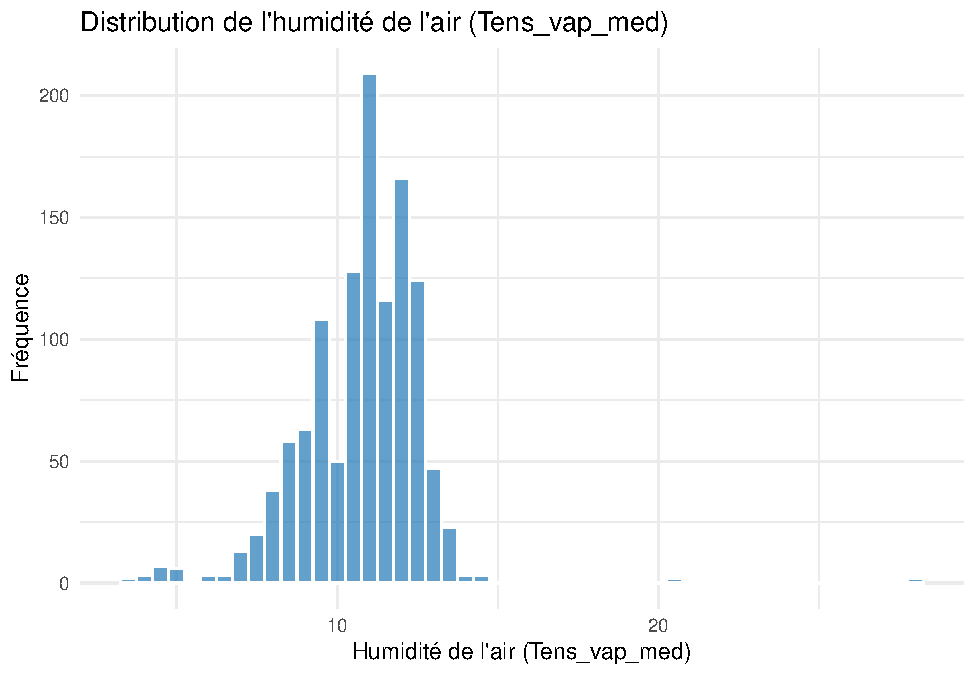
\includegraphics{Rapport_files/figure-latex/unnamed-chunk-1-1.pdf}

Dans cette étude descriptive, nous avons élaboré un graphique à barres
illustrant la distribution des diverses catégories d'incendies
primaires.

Nous avons intégré les bibliothèques \textbf{tidyverse},
\textbf{ggplot2}, \textbf{dplyr}, \textbf{ggpubr} et \textbf{corrplot}
pour effectuer des analyses et visualisations de données. Ensuite, nous
avons importé les données du fichier.

Nous avons sélectionné les données en omettant les valeurs absentes dans
la colonne \textbf{nature\_inc\_prim}.

Nous avons par la suite dénombré le nombre d'apparitions pour chaque
sorte de feu principal.

Nous avons déterminé le taux relatif en pourcentage pour chaque
catégorie.

Nous élaborons un diagramme à barres avec \textbf{ggplot2} où l'axe X
représente les catégories d'incendies classées par ordre de fréquence
décroissante.

L'axe des Y représente le nombre d'incendies.

Chaque barre est teintée en fonction du genre d'incendie à l'aide de la
palette « Dark2 ».

Les pourcentages sont présentés au-dessus de chaque barre.

Cette analyse descriptive univariée vise à compter les occurrences et le
pourcentage de chaque type d'incendie. Le résultat sera un tableau
présentant les effectifs et les fréquences.

Ensuite, pour visualiser nos résultats, nous représentons la
distribution des incendies primaires à travers des diagrammes en barres.

\subparagraph{4.2.1.2 Analyse de
nature\_sec\_inc:}\label{analyse-de-nature_sec_inc}

\begin{Shaded}
\begin{Highlighting}[]
\FunctionTok{library}\NormalTok{(tidyverse)}
\FunctionTok{library}\NormalTok{(ggplot2)}
\FunctionTok{library}\NormalTok{(dplyr)}
\FunctionTok{library}\NormalTok{(ggpubr)}
\FunctionTok{library}\NormalTok{(corrplot)}

\CommentTok{\# Charger les données}
\NormalTok{df }\OtherTok{\textless{}{-}} \FunctionTok{read.csv}\NormalTok{(}\StringTok{"../Data/donnees\_incendies.csv"}\NormalTok{)}

\NormalTok{df\_summary }\OtherTok{\textless{}{-}}\NormalTok{ df }\SpecialCharTok{\%\textgreater{}\%} 
  \FunctionTok{filter}\NormalTok{(}\SpecialCharTok{!}\FunctionTok{is.na}\NormalTok{(nature\_inc\_sec)) }\SpecialCharTok{\%\textgreater{}\%}  \CommentTok{\# Exclure les NA}
  \FunctionTok{count}\NormalTok{(nature\_inc\_sec) }\SpecialCharTok{\%\textgreater{}\%}
  \FunctionTok{mutate}\NormalTok{(}\AttributeTok{freq =}\NormalTok{ n }\SpecialCharTok{/} \FunctionTok{sum}\NormalTok{(n) }\SpecialCharTok{*} \DecValTok{100}\NormalTok{)}

\FunctionTok{ggplot}\NormalTok{(df\_summary, }\FunctionTok{aes}\NormalTok{(}\AttributeTok{x =} \FunctionTok{reorder}\NormalTok{(nature\_inc\_sec, }\SpecialCharTok{{-}}\NormalTok{n), }\AttributeTok{y =}\NormalTok{ n, }\AttributeTok{fill =}\NormalTok{ nature\_inc\_sec)) }\SpecialCharTok{+} 
  \FunctionTok{geom\_bar}\NormalTok{(}\AttributeTok{stat =} \StringTok{"identity"}\NormalTok{, }\AttributeTok{show.legend =} \ConstantTok{FALSE}\NormalTok{) }\SpecialCharTok{+}
  \FunctionTok{geom\_text}\NormalTok{(}\FunctionTok{aes}\NormalTok{(}\AttributeTok{label =} \FunctionTok{paste0}\NormalTok{(}\FunctionTok{round}\NormalTok{(freq, }\DecValTok{1}\NormalTok{), }\StringTok{"\%"}\NormalTok{)), }\AttributeTok{vjust =} \SpecialCharTok{{-}}\FloatTok{0.5}\NormalTok{, }\AttributeTok{size =} \DecValTok{4}\NormalTok{) }\SpecialCharTok{+}
  \FunctionTok{scale\_fill\_brewer}\NormalTok{(}\AttributeTok{palette =} \StringTok{"Set2"}\NormalTok{) }\SpecialCharTok{+}
  \FunctionTok{labs}\NormalTok{(}
    \AttributeTok{title =} \StringTok{"Répartition des types d\textquotesingle{}incendies (secondaires) sans NA"}\NormalTok{, }
    \AttributeTok{x =} \StringTok{"Type d\textquotesingle{}incendie"}\NormalTok{,}
    \AttributeTok{y =} \StringTok{"Nombre d\textquotesingle{}incidents"}
\NormalTok{  ) }\SpecialCharTok{+}
  \FunctionTok{theme\_minimal}\NormalTok{() }\SpecialCharTok{+}
  \FunctionTok{theme}\NormalTok{(}
    \AttributeTok{plot.title =} \FunctionTok{element\_text}\NormalTok{(}\AttributeTok{hjust =} \FloatTok{0.5}\NormalTok{, }\AttributeTok{face =} \StringTok{"bold"}\NormalTok{, }\AttributeTok{size =} \DecValTok{14}\NormalTok{),}
    \AttributeTok{axis.text.x =} \FunctionTok{element\_text}\NormalTok{(}\AttributeTok{angle =} \DecValTok{45}\NormalTok{, }\AttributeTok{hjust =} \DecValTok{1}\NormalTok{)}
\NormalTok{  )}
\end{Highlighting}
\end{Shaded}

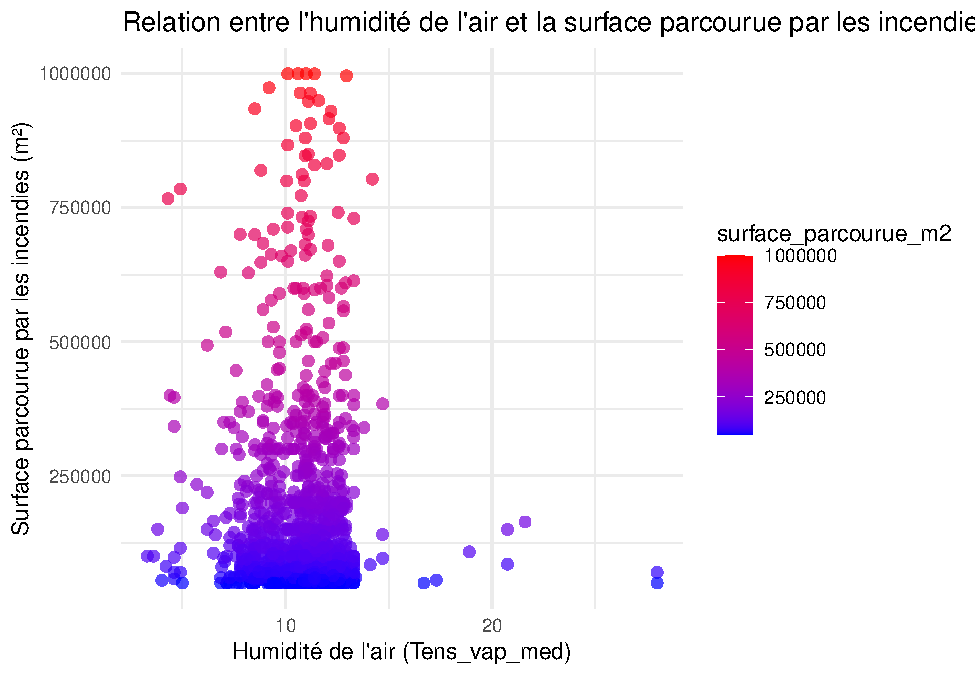
\includegraphics{Rapport_files/figure-latex/unnamed-chunk-2-1.pdf}

Dans le cadre de cette étude, nous avons élaboré un graphique à barres
qui montre la distribution des divers genres d'incendies secondaires.

D'abord, on importe les bibliothèques nécessaires pour l'analyse et la
visualisation. Les informations ont été extraites à partir du fichier
\textbf{donnees\_incendies.Csv}.

Nous avons procédé à un filtrage des données pour éliminer les valeurs
absentes dans la colonne \textbf{nature\_inc\_sec}. Chaque type
d'incendie secondaire a été quantifié et la fréquence proportionnelle en
pourcentage a été déterminée pour chaque catégorie.

Un graphique à barres a été élaboré à l'aide de la bibliothèque
\textbf{ggplot2}, où l'axe des \textbf{X} illustre les catégories
d'incendies secondaires ordonnées en fonction de leur fréquence
décroissante.

L'axe vertical représente le nombre d'incendies.

Chaque barre est teintée en fonction de la catégorie d'incendies en
utilisant la palette \textbf{Set2}. Les taux sont présentés au-dessus de
chaque barre.

Le but de cette étude est de dénombrer les incendies par cause
secondaire, puis de déterminer les fréquences relatives et d'illustrer
la distribution des causes secondaires à l'aide d'un diagramme en
barres.

\subparagraph{4.2.1.3 Analyse de Mois:}\label{analyse-de-mois}

\begin{Shaded}
\begin{Highlighting}[]
\NormalTok{df }\OtherTok{\textless{}{-}} \FunctionTok{read.csv}\NormalTok{(}\StringTok{"../Data/donnees\_incendies.csv"}\NormalTok{)}
\NormalTok{df\_summary\_mois }\OtherTok{\textless{}{-}}\NormalTok{ df }\SpecialCharTok{\%\textgreater{}\%}
  \FunctionTok{filter}\NormalTok{(}\SpecialCharTok{!}\FunctionTok{is.na}\NormalTok{(mois)) }\SpecialCharTok{\%\textgreater{}\%}
  \FunctionTok{count}\NormalTok{(mois) }\SpecialCharTok{\%\textgreater{}\%}
  \FunctionTok{mutate}\NormalTok{(}\AttributeTok{freq =}\NormalTok{ n }\SpecialCharTok{/} \FunctionTok{sum}\NormalTok{(n) }\SpecialCharTok{*} \DecValTok{100}\NormalTok{)}

\CommentTok{\# Convertir la colonne "mois" en facteur ordonné}
\NormalTok{df\_summary\_mois}\SpecialCharTok{$}\NormalTok{mois }\OtherTok{\textless{}{-}} \FunctionTok{factor}\NormalTok{(df\_summary\_mois}\SpecialCharTok{$}\NormalTok{mois, }
                               \AttributeTok{levels =} \FunctionTok{c}\NormalTok{(}\StringTok{"Jan"}\NormalTok{, }\StringTok{"Feb"}\NormalTok{, }\StringTok{"Mar"}\NormalTok{, }\StringTok{"Apr"}\NormalTok{, }\StringTok{"May"}\NormalTok{, }\StringTok{"Jun"}\NormalTok{, }
                                          \StringTok{"Jul"}\NormalTok{, }\StringTok{"Aug"}\NormalTok{, }\StringTok{"Sep"}\NormalTok{, }\StringTok{"Oct"}\NormalTok{, }\StringTok{"Nov"}\NormalTok{, }\StringTok{"Dec"}\NormalTok{))}

\FunctionTok{ggplot}\NormalTok{(df\_summary\_mois, }\FunctionTok{aes}\NormalTok{(}\AttributeTok{x =}\NormalTok{ mois, }\AttributeTok{y =}\NormalTok{ n, }\AttributeTok{fill =}\NormalTok{ mois)) }\SpecialCharTok{+} 
  \FunctionTok{geom\_bar}\NormalTok{(}\AttributeTok{stat =} \StringTok{"identity"}\NormalTok{, }\AttributeTok{show.legend =} \ConstantTok{FALSE}\NormalTok{) }\SpecialCharTok{+}
  \FunctionTok{geom\_text}\NormalTok{(}\FunctionTok{aes}\NormalTok{(}\AttributeTok{label =}\NormalTok{ n), }\AttributeTok{vjust =} \SpecialCharTok{{-}}\FloatTok{0.5}\NormalTok{, }\AttributeTok{size =} \DecValTok{4}\NormalTok{) }\SpecialCharTok{+}
  \FunctionTok{scale\_fill\_brewer}\NormalTok{(}\AttributeTok{palette =} \StringTok{"Set3"}\NormalTok{) }\SpecialCharTok{+}
  \FunctionTok{labs}\NormalTok{(}
    \AttributeTok{title =} \StringTok{"Répartition des incendies par mois"}\NormalTok{,}
    \AttributeTok{x =} \StringTok{"Mois"}\NormalTok{,}
    \AttributeTok{y =} \StringTok{"Nombre d\textquotesingle{}incendies"}
\NormalTok{  ) }\SpecialCharTok{+}
  \FunctionTok{theme\_minimal}\NormalTok{() }\SpecialCharTok{+}
  \FunctionTok{theme}\NormalTok{(}
    \AttributeTok{plot.title =} \FunctionTok{element\_text}\NormalTok{(}\AttributeTok{hjust =} \FloatTok{0.5}\NormalTok{, }\AttributeTok{face =} \StringTok{"bold"}\NormalTok{, }\AttributeTok{size =} \DecValTok{14}\NormalTok{)}
\NormalTok{  )}
\end{Highlighting}
\end{Shaded}

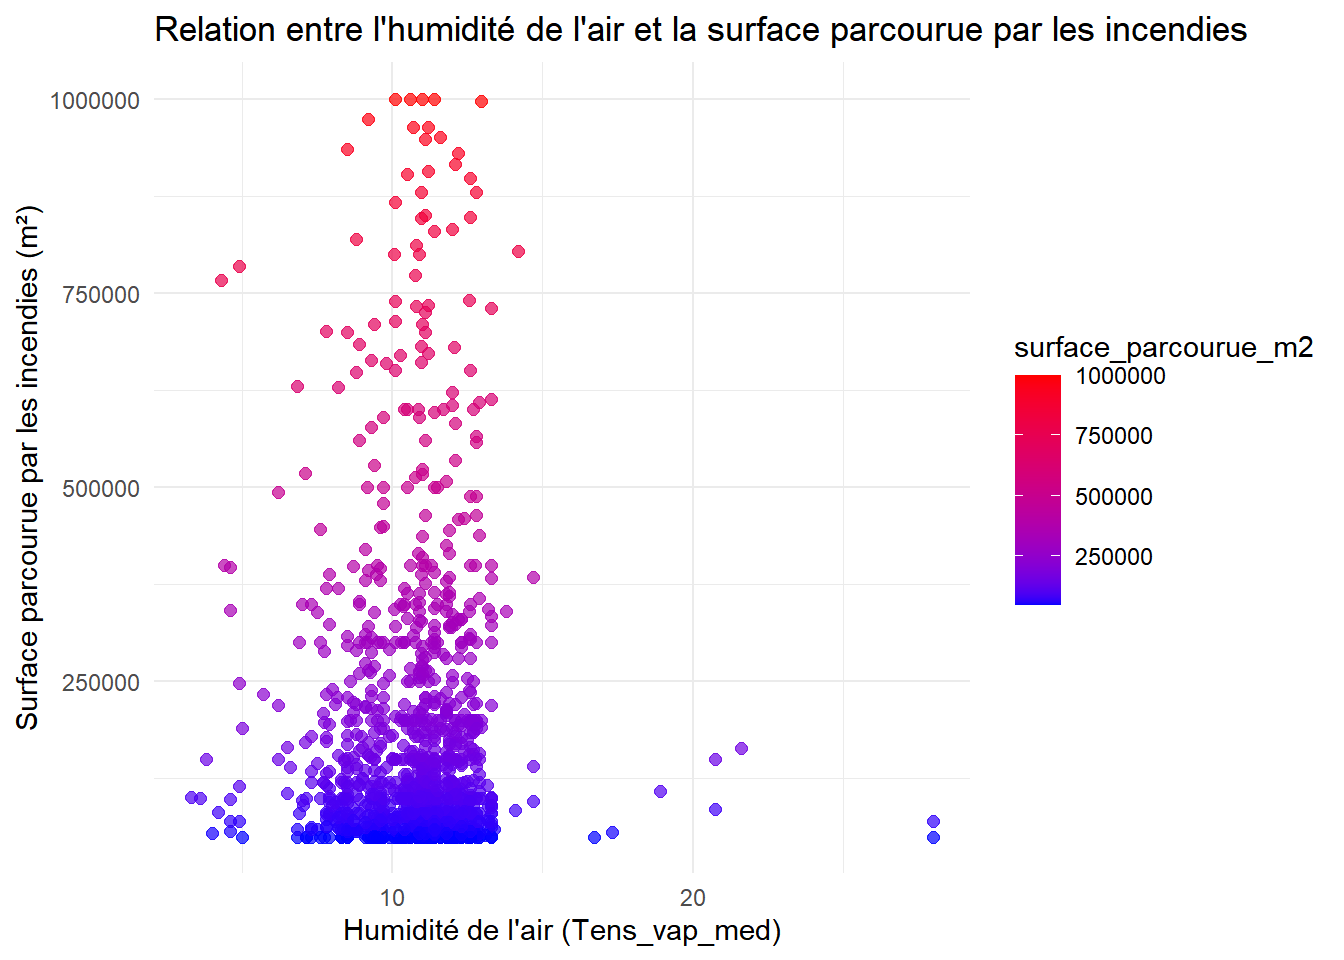
\includegraphics{Rapport_files/figure-latex/unnamed-chunk-3-1.pdf}

Dans ce travail d'analyse, nous allons réaliser un graphique à barres.
En premier lieu, nous importons les données du fichier
\textbf{donnees\_incendies.csv}, avant de procéder à la sélection des
données afin d'éliminer les valeurs absentes dans la colonne
\textbf{mois}.

Par la suite, le nombre d'incendies pour chaque mois a été enregistré.

Le calcul de la fréquence relative en pourcentage a été effectué pour
chaque mois.

Pour assurer une présentation chronologique, nous transformons la
colonne mois en facteur ordonné afin que les mois soient affichés dans
leur ordre naturel.

On a employé les abréviations des mois comme niveaux du facteur.

On génère ensuite le graphique à l'aide de la bibliothèque
\textbf{ggplot2}, en précisant que l'axe X représente les mois dans leur
séquence chronologique et l'axe Y indique le nombre d'incendies.

Chaque barre est teintée en fonction du mois selon la palette
\textbf{Set3}.

Le chiffre précis des incendies est présenté au-dessus de chaque barre.

Cette étude vise à démontrer la répartition saisonnière des incendies,
nous permettant ainsi d'identifier les pics saisonniers.

Il est essentiel de noter que \textbf{factor(mois)} est utilisé pour que
les mois soient considérés comme \textbf{catégories} plutôt que comme
chiffres.

\subparagraph{4.2.1.4 Analyse des communes les plus
touches:}\label{analyse-des-communes-les-plus-touches}

\begin{Shaded}
\begin{Highlighting}[]
\NormalTok{df }\SpecialCharTok{\%\textgreater{}\%} \FunctionTok{count}\NormalTok{(commune) }\SpecialCharTok{\%\textgreater{}\%} \FunctionTok{arrange}\NormalTok{(}\FunctionTok{desc}\NormalTok{(n)) }\SpecialCharTok{\%\textgreater{}\%} \FunctionTok{head}\NormalTok{(}\DecValTok{10}\NormalTok{)}
\end{Highlighting}
\end{Shaded}

\begin{verbatim}
##                commune  n
## 1               Oletta 16
## 2          Ghisonaccia 10
## 3  Castello-di-Rostino  9
## 4            Lantosque  9
## 5         Linguizzetta  9
## 6                Calce  7
## 7    Salses-le-Château  7
## 8              Ajaccio  6
## 9            Montbazin  6
## 10               Rosis  6
\end{verbatim}

Avec cette commande, nous pouvons déterminer les 10 communes qui ont
enregistré le plus d'incendies.

C'est une étude géographique qui nous permettra de savoir où les
incendies sont les plus courants.

\paragraph{4.2.2 Analyse sur les Varibales
Quantitatives}\label{analyse-sur-les-varibales-quantitatives}

\begin{Shaded}
\begin{Highlighting}[]
\CommentTok{\# Charger les données}
\NormalTok{df }\OtherTok{\textless{}{-}} \FunctionTok{read.csv}\NormalTok{(}\StringTok{"../Data/donnees\_incendies.csv"}\NormalTok{)}

\CommentTok{\# Variables quantitatives}
\NormalTok{vars\_quanti }\OtherTok{\textless{}{-}} \FunctionTok{c}\NormalTok{(}\StringTok{"surface\_parcourue\_m2"}\NormalTok{, }\StringTok{"annee"}\NormalTok{, }\StringTok{"mois"}\NormalTok{, }\StringTok{"jour"}\NormalTok{, }\StringTok{"heure"}\NormalTok{)}

\CommentTok{\# Statistiques descriptives globales}
\FunctionTok{summary}\NormalTok{(df[vars\_quanti])}
\end{Highlighting}
\end{Shaded}

\begin{verbatim}
##  surface_parcourue_m2     annee          mois                jour      
##  Min.   :  50000      Min.   :2012   Length:1202        Min.   : 1.00  
##  1st Qu.:  69519      1st Qu.:2015   Class :character   1st Qu.: 8.00  
##  Median : 102831      Median :2017   Mode  :character   Median :16.00  
##  Mean   : 179540      Mean   :2018                      Mean   :15.64  
##  3rd Qu.: 204950      3rd Qu.:2021                      3rd Qu.:23.00  
##  Max.   :1000000      Max.   :2022                      Max.   :31.00  
##      heure      
##  Min.   : 0.00  
##  1st Qu.:12.00  
##  Median :14.00  
##  Mean   :13.89  
##  3rd Qu.:16.00  
##  Max.   :23.00
\end{verbatim}

Dans cette section, nous avons réalisé une analyse statistique univariée
basée sur des variables quantitatives, en employant les variables
suivantes :

\begin{itemize}
\tightlist
\item
  \textbf{surface\_parcourue\_m2}: la surface parcourue par l'incendie
\item
  \textbf{annee} : l'annee de l'incendie
\item
  \textbf{mois} : le mois de l'incendie
\item
  \textbf{jour} : le jour de l'incendie
\item
  \textbf{heure} : l'heure de l'incendie
\end{itemize}

Pour ce faire, nous avons utilisé la fonction \textbf{summary()} pour
obtenir les principales mesures de tendance centrale et de dispersion
pour chaque variable, comme le minimum, le maximum, etc.

Nous examinerons ces chiffres plus en profondeur dans la cinquième
section de notre rapport.

\subsubsection{4.2 Analyse Descriptive
Bivariees}\label{analyse-descriptive-bivariees}

\paragraph{4.2.1 Quali vs Quali}\label{quali-vs-quali}

\begin{Shaded}
\begin{Highlighting}[]
\FunctionTok{library}\NormalTok{(ggplot2)}
\FunctionTok{library}\NormalTok{(dplyr)}
\NormalTok{df }\OtherTok{\textless{}{-}} \FunctionTok{read.csv}\NormalTok{(}\StringTok{"../Data/donnees\_incendies.csv"}\NormalTok{)}

\CommentTok{\# Tableau croisé}
\FunctionTok{table}\NormalTok{(df}\SpecialCharTok{$}\NormalTok{nature\_inc\_prim, df}\SpecialCharTok{$}\NormalTok{nature\_inc\_sec)}
\end{Highlighting}
\end{Shaded}

\begin{verbatim}
##               
##                particulier travaux
##   Accidentelle           0       0
##   Involontaire         221     282
##   Malveillance           0       0
##   Naturelle              0       0
\end{verbatim}

\begin{Shaded}
\begin{Highlighting}[]
\CommentTok{\# Test du Chi²}
\FunctionTok{chisq.test}\NormalTok{(}\FunctionTok{table}\NormalTok{(df}\SpecialCharTok{$}\NormalTok{nature\_inc\_prim, df}\SpecialCharTok{$}\NormalTok{nature\_inc\_sec))}
\end{Highlighting}
\end{Shaded}

\begin{verbatim}
## Warning in chisq.test(table(df$nature_inc_prim, df$nature_inc_sec)):
## Chi-squared approximation may be incorrect
\end{verbatim}

\begin{verbatim}
## 
##  Pearson's Chi-squared test
## 
## data:  table(df$nature_inc_prim, df$nature_inc_sec)
## X-squared = NaN, df = 3, p-value = NA
\end{verbatim}

\begin{Shaded}
\begin{Highlighting}[]
\NormalTok{df }\SpecialCharTok{\%\textgreater{}\%}
  \FunctionTok{filter}\NormalTok{(}\SpecialCharTok{!}\FunctionTok{is.na}\NormalTok{(nature\_inc\_sec)) }\SpecialCharTok{\%\textgreater{}\%}
  \FunctionTok{ggplot}\NormalTok{(}\FunctionTok{aes}\NormalTok{(}\AttributeTok{x =}\NormalTok{ nature\_inc\_prim, }\AttributeTok{fill =}\NormalTok{ nature\_inc\_sec)) }\SpecialCharTok{+} 
  \FunctionTok{geom\_bar}\NormalTok{(}\AttributeTok{position =} \StringTok{"dodge"}\NormalTok{) }\SpecialCharTok{+}
  \FunctionTok{scale\_fill\_brewer}\NormalTok{(}\AttributeTok{palette =} \StringTok{"Set3"}\NormalTok{) }\SpecialCharTok{+}  \CommentTok{\# Palette plus colorée}
  \FunctionTok{theme\_minimal}\NormalTok{() }\SpecialCharTok{+}
  \FunctionTok{theme}\NormalTok{(}
    \AttributeTok{plot.title =} \FunctionTok{element\_text}\NormalTok{(}\AttributeTok{size =} \DecValTok{14}\NormalTok{, }\AttributeTok{face =} \StringTok{"bold"}\NormalTok{),}
    \AttributeTok{axis.text.x =} \FunctionTok{element\_text}\NormalTok{(}\AttributeTok{angle =} \DecValTok{45}\NormalTok{, }\AttributeTok{hjust =} \DecValTok{1}\NormalTok{)}
\NormalTok{  ) }\SpecialCharTok{+}
  \FunctionTok{labs}\NormalTok{(}
    \AttributeTok{title =} \StringTok{"Répartition des types d\textquotesingle{}incendies (primaire vs secondaire)"}\NormalTok{,}
    \AttributeTok{x =} \StringTok{"Nature primaire"}\NormalTok{,}
    \AttributeTok{fill =} \StringTok{"Nature secondaire"}
\NormalTok{  )}
\end{Highlighting}
\end{Shaded}

\includegraphics{Rapport_files/figure-latex/unnamed-chunk-6-1.pdf}

Dans cette étude, nous avons initialement effectué un tableau croisé
entre les catégories d'incendies primaires et secondaires afin
d'examiner le lien entre ces deux variables de nature qualitative.

Par la suite, nous avons effectué un test du Chi² d'indépendance afin de
déterminer s'il existe une corrélation statistique entre les
caractéristiques des incendies primaires et secondaires.

Pour mettre en évidence cette relation de manière visuelle, nous avons
créé un graphique à barres groupées (barplot en « dodge »), omettant les
valeurs manquantes (NA) de la variable secondaire.

Le graphique adopte une gamme de couleurs éclatantes (Set3) afin de
différencier clairement les diverses catégories d'incendies secondaires,
tout en présentant un design sobre et des libellés clairs sur l'axe
horizontal.

Cette démarche permet de combiner à la fois une analyse statistique et
une visualisation claire pour mieux comprendre la distribution conjointe
des deux types d'incendies.

\subsection{5. Partie Analyse des
Donees}\label{partie-analyse-des-donees}

\subsubsection{5.1 Definitions des concepts
statistiques}\label{definitions-des-concepts-statistiques}

Avant de commencer à donner des définitions, il est essentiel de nous
baser sur le concept initial, c'est-à-dire la définition du terme
Statistique. On peut définir ou représenter la statistique comme
l'ensemble des méthodes et techniques utilisées pour collecter,
analyser, interpréter et présenter des données numériques.

Dans ce projet, nous allons nous concentrer sur la branche des
statistiques connue sous le nom de Statistique Inférentielle.

La statistique inférentielle est une discipline des statistiques qui
s'appuie sur les données d'un échantillon pour formuler des déductions
ou effectuer des généralisations à propos d'une population plus vaste.

À l'opposé de la statistique descriptive qui se concentre sur le résumé
ou la description des traits d'un ensemble de données, la statistique
inférentielle offre la possibilité de réaliser des estimations et des
tests concernant les paramètres d'une population basée sur des données
issues d'un échantillon. Elle s'appuie sur la théorie des probabilités,
ce qui rend possible des inférences rigoureuses et quantifiables.

Nous allons définir ci-dessus certains concepts statistiques que nous
utiliserons dans notre analyse statistique.

\textbf{Définition de la Moyenne}

La \textbf{moyenne arithmétique} d'un ensemble de données est une mesure
de tendance centrale qui représente la valeur moyenne autour de laquelle
les observations se répartissent. Elle est définie comme le quotient de
la somme des valeurs observées par le nombre total d'observations.

Soit un échantillon \(X = \{x_1, x_2, ..., x_n\}\) de taille \(n\), la
moyenne \(\bar{X}\) est donnée par :

\[
\bar{X} = \frac{1}{n} \sum_{i=1}^{n} x_i
\]

Cette mesure est sensible aux valeurs extrêmes et est couramment
utilisée en \textbf{statistique descriptive} pour résumer un ensemble de
données.

\textbf{Définition de la Médiane}

En statistique, la \textbf{médiane} est une mesure de tendance centrale
qui divise une distribution ordonnée en deux sous-ensembles de même
effectif. Elle est définie comme la valeur \(M\) telle que :

\begin{itemize}
\tightlist
\item
  \textbf{50 \% des observations sont inférieures ou égales à \(M\)}\\
\item
  \textbf{50 \% des observations sont supérieures ou égales à \(M\)}
\end{itemize}

Mathématiquement, soit un échantillon de taille \(n\) constitué des
observations \textbf{\(x_1, x_2, ..., x_n\)} classées par ordre
croissant :

\begin{itemize}
\tightlist
\item
  \textbf{Si \(n\) est impair} \((n = 2k + 1)\), la médiane est
  l'élément central :
\end{itemize}

\[
M = x_{k+1}
\]

\begin{itemize}
\tightlist
\item
  \textbf{Si \(n\) est pair} \((n = 2k)\), la médiane est la moyenne des
  deux valeurs centrales :
\end{itemize}

\[
M = \frac{x_k + x_{k+1}}{2}
\]

\textbf{Définition de la Variance:}

La \textbf{variance} mesure la dispersion des données par rapport à la
moyenne.

Plus la variance est élevée, plus les données sont dispersées.

\[
\text{Var}(X) = \frac{1}{n} \sum_{i=1}^{n}(x_i - \bar{x})^2
\]

\textbf{Définition de l'Écart-type (σ):}

L'\textbf{écart-type} est la racine carrée de la variance.\\
Il exprime la dispersion des données dans la même unité que les valeurs
initiales.

\[
\sigma = \sqrt{\text{Var}(X)}
\] \textbf{Définition de la Classe Modale}

La \textbf{classe modale} est l'intervalle de valeurs qui renferme le
plus fort effectif dans une distribution organisée en classes. Autrement
dit, c'est la classe qui se manifeste le plus souvent dans un
histogramme.

\textbf{Définition de ggplot2}

ggplot est une des librairies du langage R. Elle fait partie du package
plotnine, qui facilite la création de graphiques.

\textbf{Définition de la Population}

En statistique, la population se réfère à l'ensemble de tous les
individus, objets ou événements qui sont sujets à une étude.

\textbf{Définition d'un Échantillon}

Un échantillon représente une partie de la population étudiée. On fait
appel à lui quand il est nécessaire d'analyser l'ensemble de la
population en raison de sa complexité.

\textbf{Définition d'une Variable}

Une variable est un attribut quantifiable qui peut varier d'un individu
à l'autre.

\textbf{Définition d'une variable qualitative}

Une variable qualitative représente une caractéristique ou une catégorie
qui ne peut pas être quantifiée.

\textbf{Définition d'une variable quantitative}

Une Variable Quantitative représente une évaluation numérique et peut
être l'objet d'opérations mathématiques.

\textbf{Définition d'un Intervalle de Confiance}

Un intervalle de confiance c'est l'outil qui nous permet d'estimer une
plage dans laquelle une valeur inconnue comme une moyenne ou une
proportion se situe avec un certain niveau de confiance.

\textbf{Définition du test du khi deux (χ²):}

Le \textbf{test du khi deux (χ²)} est un test statistique utilisé pour
déterminer s'il existe une association significative entre deux
variables qualitatives. Il est basé sur la comparaison entre des
\textbf{fréquences observées} et des \textbf{fréquences théoriques}
attendues selon une hypothèse nulle.

\[
\chi^2 = \sum \frac{(O_i - E_i)^2}{E_i}
\] où : - \(O_i\) est la fréquence observée, - \(E_i\) est la fréquence
attendue.

\textbf{Test de Student (t de Student):}

Le \textbf{test de Student} est utilisé pour comparer des
\textbf{moyennes} entre deux groupes et déterminer s'il existe une
différence statistiquement significative.

\begin{itemize}
\tightlist
\item
  \textbf{Test t pour un échantillon} : comparer la moyenne d'un
  échantillon à une valeur théorique.
\item
  \textbf{Test t pour échantillons indépendants} : comparer les moyennes
  de deux groupes indépendants.
\item
  \textbf{Test t pour échantillons appariés} : comparer les moyennes de
  deux mesures faites sur les mêmes individus.
\end{itemize}

\[
t = \frac{\bar{X}_1 - \bar{X}_2}{\sqrt{\frac{s_1^2}{n_1} + \frac{s_2^2}{n_2}}}
\]

\textbf{Test de Normalité (loi normale):}

Le \textbf{test de normalité} sert à vérifier si un jeu de données suit
une \textbf{distribution normale}, ce qui est une condition préalable
pour de nombreux tests paramétriques.

\begin{itemize}
\tightlist
\item
  Si la \textbf{p-valeur} est \textless{} 0.05, on rejette l'hypothèse
  de normalité (distribution non normale).
\item
  Si la \textbf{p-valeur} est ≥ 0.05, on considère la distribution comme
  normale.
\end{itemize}

\textbf{Hypothèse nulle (H₀):}

L'\textbf{hypothèse nulle (H₀)} est une affirmation de départ selon
laquelle il n'y a \textbf{pas d'effet}, \textbf{pas de différence}, ou
\textbf{pas de lien} entre les variables.

Les tests statistiques cherchent à vérifier si cette hypothèse peut être
rejetée.

\textbf{Hypothèse alternative (H₁):}

L'\textbf{hypothèse alternative (H₁)} est l'hypothèse opposée à
l'hypothèse nulle.\\
Elle affirme qu'il existe \textbf{un effet}, \textbf{une différence}, ou
\textbf{une relation} statistiquement significative.

\textbf{Loi Normale:}

La \textbf{loi normale} (ou loi de Gauss) est une distribution de
probabilité symétrique en forme de cloche.\\
Elle est définie par deux paramètres : la moyenne \(\mu\) et l'écart
type \(\sigma\).\\
Elle est fondamentale dans les statistiques pour les tests
paramétriques.

\textbf{Test paramétrique:}

Un \textbf{test paramétrique} suppose que les données suivent une
certaine distribution (souvent normale) et utilisent des paramètres
comme la moyenne et l'écart-type.

\textbf{Test non paramétrique:}

Un \textbf{test non paramétrique} ne repose pas sur des hypothèses
fortes concernant la distribution des données.\\
Exemples : test de Wilcoxon, test de Mann-Whitney.

\textbf{Corrélation:}

La \textbf{corrélation} mesure la force et la direction d'une relation
linéaire entre deux variables quantitatives.\\
Elle est exprimée par un coefficient \(r\) entre -1 et 1.

\textbf{Régression:}

La \textbf{régression} est une méthode statistique permettant de
modéliser la relation entre une variable dépendante et une ou plusieurs
variables indépendantes.

\textbf{Distribution binomiale:}

La \textbf{distribution binomiale} décrit le nombre de succès dans une
séquence de \textbf{n essais indépendants} où chaque essai a une
probabilité constante de succès.

Elle est utilisée pour des variables discrètes.

\subsubsection{5.2 Description des
donnees}\label{description-des-donnees}

Avant de procéder à l'étude détaillée des données et à leur
représentation graphique, il est essentiel de saisir la nature des
informations fournies par nos éducateurs.

Ces données constitueront le fondement de notre analyse, et leur examen
devra être mené avec minutie.

Les trois fichiers principaux de notre base de données sont cruciaux
pour saisir les dynamiques des incendies, leur position géographique et
les conditions environnementales associées.

Le premier document, relatif aux incendies, est probablement le plus
vital pour l'analyse de ce phénomène. Il renferme une série de
caractéristiques précisant le contexte de chaque feu.

Ces données comprennent le nom et le code de la commune, essentiels pour
situer avec précision chaque événement.

La commune n'est pas seulement une unité administrative, mais aussi un
domaine d'analyse potentiellement fructueux, car elle peut être associée
à d'autres informations géographiques pour étudier des schémas
récurrents d'incendies.

L'année et le mois de l'incendie fournissent également des indices
intéressants pour une analyse chronologique.

Effectivement, l'analyse de la fréquence des incendies sur plusieurs
années pourrait dévoiler des motifs ou des phases particulièrement
délicates, comme des saisons spécifiques où les incendies surviennent
avec une occurrence plus fréquente.

En outre, les variables concernant la date et l'heure du signalement
serviront à évaluer la réactivité des autorités en réponse à ces
incidents. Elles permettront également de mesurer la vitesse
d'intervention, un élément essentiel pour contenir l'expansion des
incendies.

Les facteurs, qu'ils soient primaires ou secondaires, qui déclenchent
les incendies constituent un autre aspect crucial pour notre examen.

L'étude des facteurs sous-jacents, qu'ils soient humains, naturels ou
liés à des phénomènes météorologiques, sera rendue possible grâce à la
compréhension de l'origine des incendies.

Cela permettra d'explorer les processus qui mènent à des situations
dangereuses et de déterminer les régions où des actions préventives
pourraient être intensifiées.

En ce qui concerne notre analyse, le fichier géographique représente une
dimension supplémentaire significative. Pour cartographier les
événements, il est crucial de disposer des informations sur la latitude,
la longitude et l'altitude des incendies.

En localisant avec exactitude chaque feu, nous pourrons les positionner
dans un espace géographique spécifique, ce qui nous offre la possibilité
d'étudier la distribution spatiale des incendies.

Cette méthode peut identifier des régions géographiques particulièrement
exposées, telles que les forêts ou les zones montagneuses, où le risque
d'incendie est plus élevé.

En outre, l'altitude pourrait aussi avoir une influence significative
sur la gravité des incendies, étant donné que les terrains élevés,
généralement plus arides, peuvent contribuer à leur extension.

Ainsi, la cartographie aidera à représenter ces éléments géographiques
et à déterminer les zones vulnérables, ce qui contribuera à la
formulation de politiques publiques axées sur la prévention.

Finalement, le fichier météo fournira une dimension additionnelle de
compréhension en offrant la possibilité d'examiner l'impact des
conditions météorologiques sur l'apparition des incendies.

Des éléments tels que la température, l'humidité, la vitesse du vent et
les précipitations peuvent directement influencer le démarrage et la
diffusion des incendies.

Par exemple, des conditions de chaleur intense couplées à un faible
niveau d'humidité peuvent favoriser un environnement susceptible de
s'enflammer, alors que des rafales puissantes pourraient contribuer à la
diffusion du feu.

Par contre, les précipitations peuvent jouer un rôle de tampon en
éteignant ou en ralentissant l'avancée du feu.

En étudiant les conditions climatiques qui prévalent lors des incendies,
nous pourrions identifier des liens entre ces éléments environnementaux
et la fréquence ou la sévérité des incendies, ce qui pourrait indiquer
des voies d'amélioration pour les stratégies de gestion des risques.

En combinant ces informations -- les propriétés des feux, leur position
géographique, et les conditions climatiques -- nous serons en mesure de
produire une analyse exhaustive et détaillée.

L'intention est de déceler des liens implicites entre les divers
éléments et d'exposer des orientations susceptibles de contribuer à une
meilleure compréhension de la dynamique des incendies.

Cette méthode globale nous donnera la possibilité non seulement de
caractériser les incendies, mais également de suggérer des mesures
concrètes pour leur prévention, leur gestion et leur réaction à ces
incidents.

L'usage de graphiques et de cartes pour l'analyse et la représentation
des données améliorera la compréhension claire de notre travail et
l'importance de nos conseils.

\subsubsection{5.3 Analyse des doneees}\label{analyse-des-doneees}

Dès que toutes les définitions et explications requises sont
rassemblées, et que notre base de données est jugée complète et
opérationnelle, nous serons en mesure d'initier l'analyse des données
par le biais du langage R.

R est un outil performant qui nous donne la possibilité de faire une
analyse détaillée et visuelle des données.

Avec sa vaste collection de fonctions et de paquets, nous serons
capables de créer une variété de graphiques, effectuer des tests
statistiques et construire des modèles qui faciliteront notre
compréhension des tendances et des motifs présents dans les données.

L'une de nos premières méthodes consistera à recourir aux histogrammes,
qui sont des instruments visuels élémentaires mais très précieux pour
étudier la répartition des diverses variables et examiner la
distribution des données.

Les histogrammes sont particulièrement utiles pour analyser la fréquence
de certains événements ou attributs.

Ces outils nous offriront la possibilité d'observer comment les valeurs
se distribuent dans chaque variable, et d'identifier des irrégularités,
des motifs saisonniers, ou des concentrations qui pourraient ne pas être
manifestes à première analyse.

Par exemple, un diagramme illustrant le nombre d'incendies selon les
années ou les mois pourrait nous permettre de vérifier s'il existe une
augmentation ou une diminution des incendies au cours du temps, ou
encore si certains mois semblent plus susceptibles d'être touchés par
des incendies que d'autres.

Ces graphiques, bien qu'ils fournissent une synthèse rapide, serviront
de point de départ pour des analyses plus détaillées, en fonction des
modèles détectés.

Nous avons organisé notre étude en divers segments distincts, chaque
segment se rapportant à une question précise que nous désirons explorer.
Chaque partie sera dirigée par une question spécifique, et les
diagrammes en barres constitueront le point de départ pour explorer
chaque facette de notre recherche.

De plus, l'emploi d'histogrammes nous offrira la possibilité d'effectuer
une analyse segmentée de façon détaillée.

Par exemple, nous pourrions établir des histogrammes afin d'analyser les
fluctuations des incendies en lien avec les conditions météorologiques,
telles que la température ou l'humidité, en mettant en parallèle les
occurrences des incendies selon diverses conditions climatiques.

Ces études visuelles, soutenues par des analyses statistiques réalisées
sur R, fourniront une perspective quantitative des liens entre les
variables et permettront de valider ou de réfuter certaines
suppositions.

Chaque histogramme, selon le problème traité, nous aide à affiner notre
interprétation des données et oriente nos pensées vers des conclusions
basées sur des preuves empiriques.

Au fil de notre examen détaillé, les histogrammes s'avéreront être des
outils cruciaux pour organiser notre pensée. Un des principaux atouts de
ces graphiques est leur capacité à offrir une analyse visuelle rapide et
pertinente, tout en apportant des éléments essentiels pour l'analyse
future, tels que la variabilité des données ou l'apparition de nouvelles
tendances.

En variant les formats d'histogrammes que nous mettrons en œuvre -- tels
que des histogrammes empilés, des histogrammes de fréquence cumulative
ou des histogrammes comparatifs -- nous parviendrons à mieux comprendre
les subtilités des liaisons entre les variables et à fournir des
réponses plus exhaustives aux interrogations posées dans chaque segment
de notre recherche.

Par conséquent, l'emploi des histogrammes dans notre étude des incendies
sera une étape cruciale orientant notre analyse.

Chaque diagramme, élaboré pour s'attaquer à une question particulière,
constituera un point de départ pour des investigations plus poussées et
des analyses à multiples variables.

Cette méthode visuelle nous permettra non seulement de repérer des
tendances ou des irrégularités, mais aussi de guider notre étude vers
des déductions significatives qui, à long terme, faciliteront
l'élaboration de solutions concrètes pour optimiser la gestion et la
prévention des incendies.

\paragraph{5.3.1 Évolution des
incendies}\label{uxe9volution-des-incendies}

\subparagraph{5.3.1.1 Évolution des incendies au fil des
années}\label{uxe9volution-des-incendies-au-fil-des-annuxe9es}

Dans cette problématique, on va interroger sur le nombre d'incendies qui
se produisent chaque année sur le territoire français. Pour répondre à
cette question, il est primordial de définir d'abord certains concepts
naturels qui faciliteront l'analyse de cette problématique. Une année se
compose de 12 mois et comporte 365 jours. Dans cette étude, nous
examinerons l'évolution annuelle du nombre d'incendies à travers tous
les départements français, déterminant s'il est en déclin ou en
ascension.

Pour réaliser cette analyse statistique, il faut utiliser la table des
\textbf{incendies}.Pour réaliser l'histogramme, nous devons utiliser le
langage R. Nous avons précisé le chemin d'accès au fichier CSV grâce à
une variable que nous avons définie, une variable donnée qui va recevoir
la fonction read.csv et le chemin du fichier. Cela permettra à la
variable d'accéder au fichier CSV. De plus, pour vérifier notre travail,
nous utiliserons la méthode head qui nous donnera les six premières
entrées de notre fichier CSV afin de nous assurer que nous travaillons
sur le bon fichier et de vérifier également l'en-tête avec les attributs
à utiliser.

Pour réaliser cette analyse, nous avons adopté cette technique qui
consiste à déterminer la fréquence des incendies par année. En d'autres
termes, nous comptabilisons le nombre d'incendies pour chaque année dans
la colonne « année » du jeu de données. Cela va nous permettre de créer
un tableau qui associe chaque année à son nombre d'incendies.

De plus, nous avons élaboré ce genre de graphique en utilisant un
graphique linéaire. Nous avons exploité la fonction « plot() » avec les
fréquences obtenues. L'option « o » a été utilisée pour indiquer que
nous allions visualiser l'évolution des incendies à la fois par des
points et des lignes sur la période donnée.

Pour adapter notre graphique à nos besoins, nous avons opté pour la
couleur bleue afin de le rendre plus personnalisable et lisible. De
plus, nous avons défini les titres des axes du graphique en utilisant
les paramètres xlab, ylab et main.

\begin{Shaded}
\begin{Highlighting}[]
\NormalTok{donnees }\OtherTok{\textless{}{-}} \FunctionTok{read.csv}\NormalTok{(}\StringTok{"../Data/donnees\_incendies.csv"}\NormalTok{)}

\NormalTok{annee\_freq }\OtherTok{\textless{}{-}} \FunctionTok{table}\NormalTok{(donnees}\SpecialCharTok{$}\NormalTok{annee)}

\FunctionTok{plot}\NormalTok{(annee\_freq, }
     \AttributeTok{type=}\StringTok{"o"}\NormalTok{,  }\CommentTok{\# "o" pour un graphique avec des points et des lignes}
     \AttributeTok{col=}\StringTok{"blue"}\NormalTok{, }
     \AttributeTok{main=}\StringTok{"Évolution des incendies au fil des années"}\NormalTok{, }
     \AttributeTok{xlab=}\StringTok{"Année"}\NormalTok{, }
     \AttributeTok{ylab=}\StringTok{"Nombre d\textquotesingle{}incendies"}\NormalTok{)}
\end{Highlighting}
\end{Shaded}

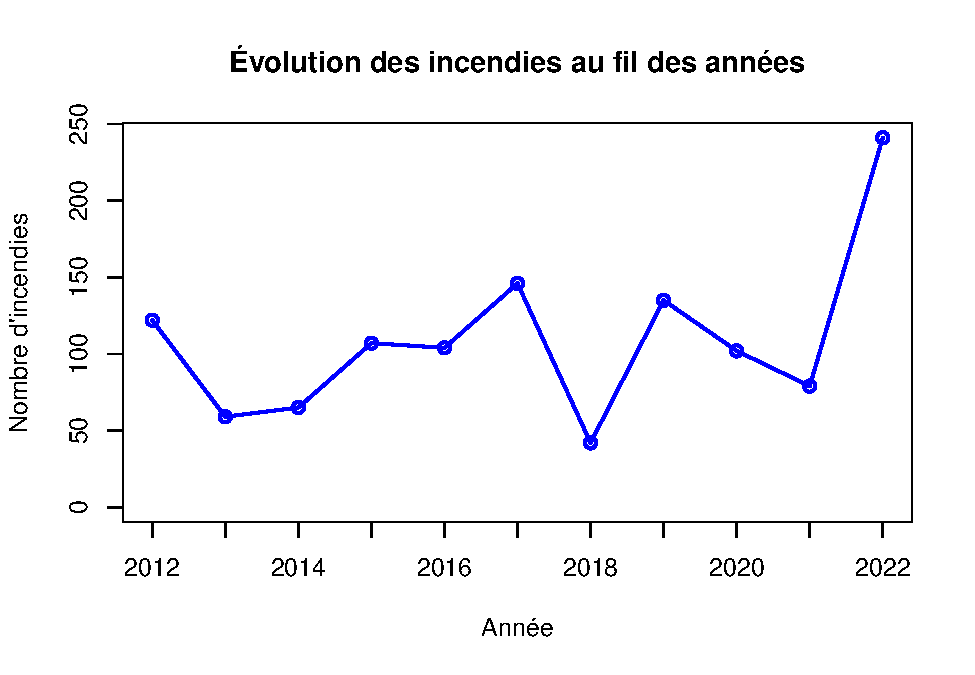
\includegraphics{Rapport_files/figure-latex/setup-1.pdf}

\begin{enumerate}
\def\labelenumi{\arabic{enumi}.}
\tightlist
\item
  \textbf{Analyse Informatique:}
\end{enumerate}

Nous allons détailler le processus de développement du code pour
structurer notre graphique. Pour cela, nous avons importé les données du
fichier grâce à la méthode \textbf{read.csv()}. Dans cette méthode, nous
avons spécifié le chemin relatif du fichier csv.Par la suite, nous avons
déterminé la fréquence des incendies par an en optant pour la colonne
\textbf{donneees\$annee}.En employant la méthode \textbf{table()}, nous
dénombrons le nombre d'incendies survenant par année.

Cela nous autorisera à constituer un tableau où les indices représentent
les années et les valeurs correspondent aux occurrences des incendies.

À présent, nous passons à la création du graphique à l'aide de la
méthode \textbf{plot()}. Nous avons indiqué la variable
\textbf{annee\_freq} et dans cette méthode, nous avons précisé le type
`o' pour indiquer que les points doivent être affichés et reliés par une
ligne. De plus, nous avons défini l'option couleur afin de spécifier que
le graphique doit être en bleu.

Avec l'option \textbf{main}, nous désignons le titre du diagramme.
Ensuite, grâce à xlab et ylab, nous définissons les étiquettes des axes
x et y, où x représente l'\textbf{année} et y représente le
\textbf{nombre d'incendies}.

\begin{enumerate}
\def\labelenumi{\arabic{enumi}.}
\setcounter{enumi}{1}
\tightlist
\item
  \textbf{Analyse Statistique:}
\end{enumerate}

Alors, débutons par cette étude ; nous allons mener notre analyse sur
une période de 11 ans, de 2012 à 2022.

Nous allons donc commencer à dresser le bilan de nos effectifs
d'incendies. En 2012, nous avons enregistré 122 incidents, en 2013, 59
incendies, en 2014, 65 incendies, en 2015, le nombre a grimpé à 107. En
2016, nous avons eu 104 incendies. Pour l'année suivante, en 2017, nous
avons connu une augmentation avec 146 incidents. Puis en 2018, le
chiffre est redescendu à 42 incendies. En 2019, nous avons rapporté 135
incendies et pour l'année suivante, en 2020 nous avions enregistré 102
incidents. Enfin pour2021 ,nous avons comptabilisé 79 incendies et
pour2022 ,le nombre d'incendies a fortement augmenté atteignant
241incendies .

Il est possible d'observer que la moyenne générale des incendies en
France sur une durée de 11 ans s'élève à 109,27. Maintenant que nous
avons compilé les totaux des onze années consécutives, nous allons
détailler notre analyse. En démarrant de 2012, nous constatons un total
de 122 incendies, ce qui pourrait être considéré comme « bon ».
Cependant, cette comparaison est prématurée tant que nous n'avons pas
répertorié les autres chiffres pour une évaluation plus approfondie.
Après une baisse de 63 incendies en 2013, on a constaté une augmentation
de 6 incendies en 2014 lors de la comparaison entre 2013 et 2014.

Cependant, en 2015, le nombre d'incendies a considérablement augmenté,
atteignant 107 incendies pour l'année 2015, ce qui représente un chiffre
élevé mais pas le plus élevé que nous ayons connu. En comparaison avec
2012, nous avons atteint un taux qui est le deuxième record maximal.
Puis en 2016, ce taux a baissé de trois incendies par rapport à l'année
précédente.

En 2017, on a observé une hausse remarquable du taux d'incendies qui a
atteint un nouveau sommet à 146, soit une augmentation de 42 incendies
par rapport à 2016. Si l'on compare avec l'année 2012, cela représente
une différence de 24 incendries. En 2018, on constate une baisse rapide
du nombre d'incendies, enregistrant un taux de 42 qui, selon les données
de 2018, représente le plus bas enregistré depuis 2012. En 2019, on a
noté une hausse significative du nombre d'incendies, atteignant 135,
soit une différence de 93 incendies par rapport à 2018.

En 2020, une baisse du nombre d'incendies entraîne une variation de 33
incendies par rapport à l'année 2029. Ensuite, on observe une baisse en
2021 avec une différence de 23 incendies par rapport à l'année 2020.
Finalement, un chiffre très élevé en 2022 a été atteint, atteignant le
nombre record de 241 incendies. De plus, cela représente une différence
de 162 incendres par rapport à l'année 2021.

On peut résumer qu'au cours de ces 11 années, l'année où le nombre
d'incendies est le plus élevé est 2022 avec un total de 241 incendies,
tandis que l'année où ce nombre est le plus bas est 2018.

En 2022, on a observé une augmentation atypique, avec un total de 241
incendies. Divers éléments peuvent expliquer cette augmentation, tels
que les modifications extrêmes des conditions météorologiques. En 2022,
des vagues de chaleur sévères et une sécheresse persistante ont
contribué à cet accroissement. De plus, les actions humaines, notamment
la négligence, ont influencé cette hausse.

Pour conclure notre analyse, l'évolution des incendies de 2012 à 2022 a
montré des tendances significatives et atypiques. Cela souligne
l'importance d'examiner l'impact des facteurs climatiques, humains et
socio-économiques sur le nombre d'incendies. On peut conclure que
l'année 2022 a été exceptionnelle, affichant le plus haut nombre
d'incendies. De plus, nous avons observé une variabilité des tendances,
comme démontré souvent avec les années 2017, 2014 et 2013 où les taux
étaient remarquablement bas comparés à ceux de 2022. Il est essentiel de
noter que le changement climatique a une grande importance.

Enfin, et c'est crucial, la gestion et la prévention jouent un rôle
primordial. Les préfectures, ainsi que les forces de police municipales
et nationales, peuvent contribuer à maîtriser ce taux d'incendies
attribués à des actes de malveillance ou de négligence.

\subparagraph{5.3.1.2 Analyse des heures
d'incendie}\label{analyse-des-heures-dincendie}

\begin{Shaded}
\begin{Highlighting}[]
\NormalTok{incendies }\OtherTok{\textless{}{-}} \FunctionTok{read.csv}\NormalTok{(}\StringTok{"../Exports/export\_incendies.csv"}\NormalTok{)}
\NormalTok{incendies}\SpecialCharTok{$}\NormalTok{heure }\OtherTok{\textless{}{-}} \FunctionTok{as.character}\NormalTok{(incendies}\SpecialCharTok{$}\NormalTok{heure)}
\NormalTok{incendies}\SpecialCharTok{$}\NormalTok{heure }\OtherTok{\textless{}{-}} \FunctionTok{as.integer}\NormalTok{(}\FunctionTok{sub}\NormalTok{(}\StringTok{":.*"}\NormalTok{, }\StringTok{""}\NormalTok{, incendies}\SpecialCharTok{$}\NormalTok{heure))}
\FunctionTok{hist}\NormalTok{(}
\NormalTok{  incendies}\SpecialCharTok{$}\NormalTok{heure, }
  \AttributeTok{main =} \StringTok{"Nombre d\textquotesingle{}incendies par heure"}\NormalTok{, }
  \AttributeTok{xlab =} \StringTok{"Heure"}\NormalTok{, }
  \AttributeTok{ylab =} \StringTok{"Nombre d\textquotesingle{}incendies"}\NormalTok{, }
  \AttributeTok{col =} \StringTok{"red"}\NormalTok{, }
  \AttributeTok{border =} \StringTok{"black"}\NormalTok{, }
  \AttributeTok{breaks =} \FunctionTok{seq}\NormalTok{(}\DecValTok{0}\NormalTok{, }\DecValTok{23}\NormalTok{, }\DecValTok{1}\NormalTok{), }
  \AttributeTok{xaxt =} \StringTok{"n"}\NormalTok{,}
  \AttributeTok{cex.axis =} \FloatTok{0.8}
\NormalTok{)}
\FunctionTok{axis}\NormalTok{(}\DecValTok{1}\NormalTok{, }\AttributeTok{at =} \FunctionTok{seq}\NormalTok{(}\DecValTok{0}\NormalTok{, }\DecValTok{23}\NormalTok{, }\DecValTok{1}\NormalTok{), }\AttributeTok{labels =} \FunctionTok{seq}\NormalTok{(}\DecValTok{0}\NormalTok{, }\DecValTok{23}\NormalTok{, }\DecValTok{1}\NormalTok{), }\AttributeTok{cex.axis =} \FloatTok{0.8}\NormalTok{)}
\end{Highlighting}
\end{Shaded}

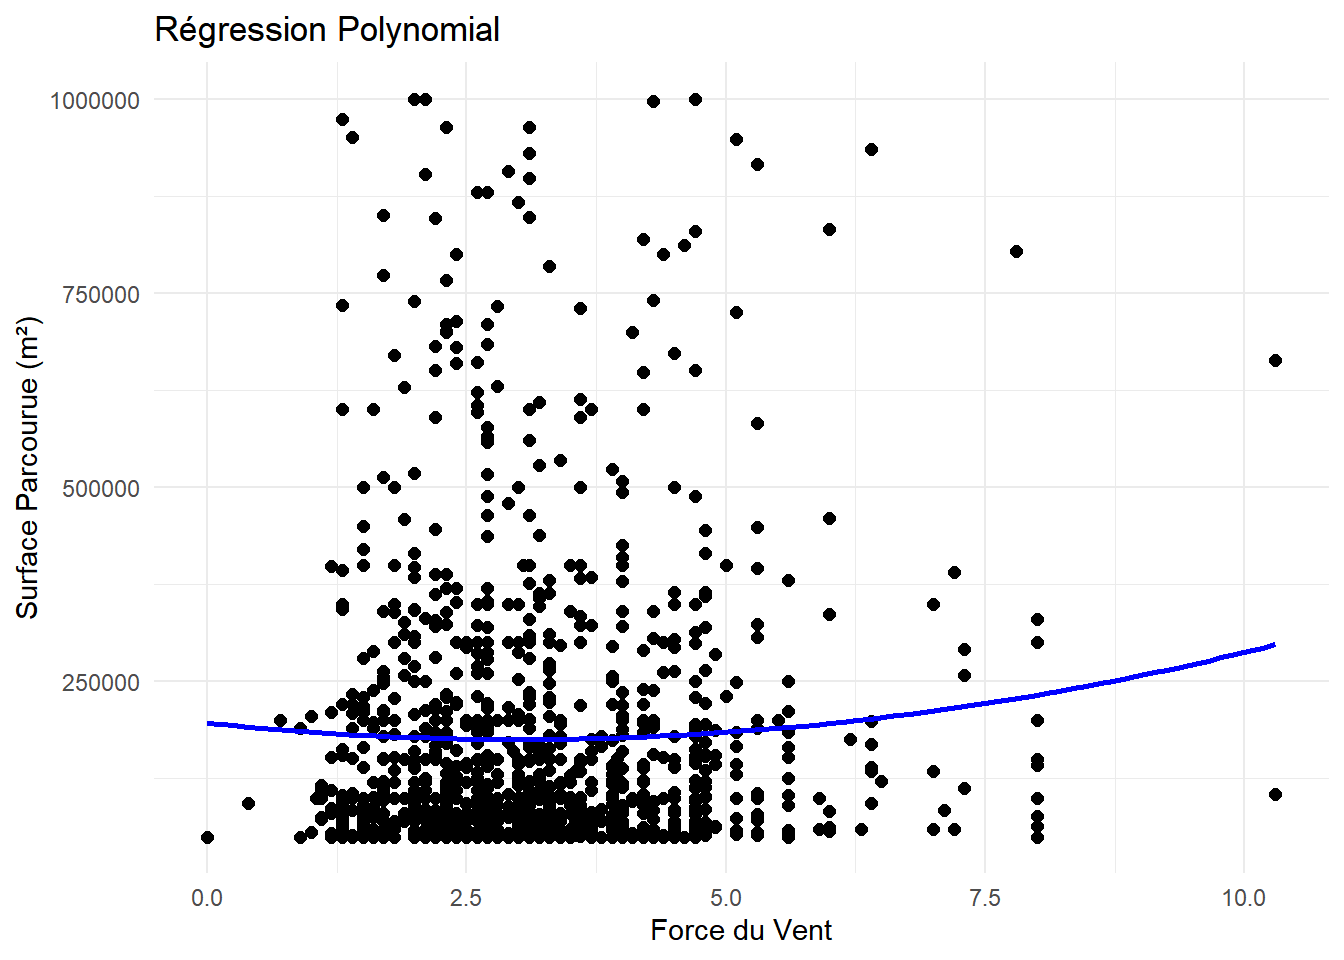
\includegraphics{Rapport_files/figure-latex/unnamed-chunk-7-1.pdf}

1- \textbf{Analyse Informatique}:

Le code débute en chargeant les données à partir du fichier CSV via
l'instruction \textbf{incendies \textless-
read.csv(``donnees\_incendies.csv'')}.

Cette étape est indispensable pour importer les données relatives aux
incendies et les organisent sous forme de tableau, un format utilisé par
R pour gérer les informations structurées.

Par la suite, nous \textbf{convertissons} la colonne de l'heure des
incendies : \textbf{incendies\(heure = as.character(incendies\)heure)}

La \textbf{colonne} doit être convertie en \textbf{chaîne de
caractères}, car certaines opérations de traitement textuel ne peuvent
se faire qu'avec ce format de données.

L'instruction suivante,
\textbf{incendies\(heure = as.integer(sub(":.", "", incendies\)heure))},
utilise la fonction \textbf{sub(``:.'', ``\,``, incendies\$heure)} pour
éliminer tout ce qui suit les deux-points « : », ne conservant ainsi que
l'heure entière.

La fonction \textbf{as.integer()} transforme par la suite cette valeur
en entier, facilitant ainsi son emploi dans \textbf{des calculs
statistiques et l'élaboration de l'histogramme.}

Par la suite, la fonction \textbf{hist()} est employée pour
\textbf{créer l'histogramme}, en utilisant
\textbf{hist(incendies\$heure,\ldots)}.

L'argument \textbf{main=``Nombre d'incendies par heure''} attribue un
titre au diagramme, alors que **xlab=``Heure*``\textbf{ et
}ylab=``Nombre d'incendies''** déterminent les désignations des axes
pour spécifier les données présentées.

L'option \textbf{col=``red''} permet de remplir les barres avec une
teinte rouge pour une distinction colorimétrique plus efficace tandis
que \textbf{border=``black''} génère des bordures noires pour délimiter
visuellement les barres.

L'option \textbf{breaks=seq(0, 23, 1)} segmente l'axe des heures en
intervalles d'une unité par barre dans le graphique, chaque barre
symbolisant une heure.

Pour finir, la commande
\textbf{axis(1,at=seq(0,23,1),labels=seq(0,23,1))} permet de
personnaliser l'axe des x. Initialement, l'option \textbf{xaxt=``n''}
dans \textbf{hist()} avait éliminé l'affichage automatique des
étiquettes sur cet axe.

Cette ligne finale ajoute \textbf{manuellement les vingt-quatre heures}
afin d'améliorer l'harmonie esthétique.

Cela garantit une clarté accrue du graphique et facilite une
interprétation optimale des données.

2- \textbf{Analyse Statistique} :

Ce graphique montre une analyse du nombre d'incendies à des heures
précises sur le \textbf{territoire français.}

On analyse la fréquence des feux sur une durée de \textbf{24 heures.}

L'axe X illustre l'ensemble des heures, de \textbf{0 à 23}, tandis que
l'axe Y représente le total des incendies, avec une portée d'environ
\textbf{0 à près de 200.}

Nous avons développé \textbf{un histogramme} comme type de graphique.

On observe un pic significatif \textbf{entre 11 heures et 14 heures},
atteignant son maximum aux alentours de \textbf{12-13} heures avec
environ \textbf{200 incendies}.\\
\textbf{Après le pic du midi}, l'occurrence des incendies commence à
décroître graduellement jusqu'à \textbf{23 heures}, avec quelques
variations mineures, comme un léger rebound autour de \textbf{18-19
heures.}

Cette répartition des données est asymétrique, montrant une queue à
droite après le pic principal de \textbf{12-13 h}, car la
\textbf{fréquence} diminue plus progressivement vers les heures tardives
\textbf{14-23 h} qu'elle ne s'accroît avant le pic.

Cette répartition indique une connexion forte entre les \textbf{actions
humaines} et les incendies.

En effet, les moments où les incendies sont le plus courants
correspondent à des périodes \textbf{d'activité humaine intense},
particulièrement entre \textbf{midi et 16h.}

Ceci pourrait être attribué à une utilisation croissante d'équipements
électriques, de cuisines ou encore de travaux dans l'industrie ou
l'agriculture, augmentant ainsi les dangers d'incendie.

L'explication de la \textbf{rareté des incendies} durant la nuit et le
matin réside dans la diminution des interactions humaines et
l'utilisation limitée de sources de chaleur et d'énergie.

Par contre, l'augmentation en pleine journée pourrait résulter des
températures estivales chaudes et de l'intensification des activités
humaines durant cette tranche horaire.

Par après 16 heures, le nombre d'incendies commence à baisser peu à peu,
ce qui peut être attribué à un ralentissement des occupations à risque
et à une prise de conscience accrue des dangers suite au pic observé.

Cependant, on note un léger rebond vers \textbf{20 heures}, probablement
associé aux tâches de fin de journée telles que la cuisine ou
l'utilisation d'appareils électriques avant le coucher.

En définitive, cette répartition horaire des incendies met en exergue
l'influence des comportements humains sur leur fréquence.

Ces données pourraient s'avérer utiles pour optimiser la prévention et
l'intervention des services d'urgence en ciblant les périodes critiques
de la journée.

Le \textbf{mode} principale se situe autour de 12-123 heures, moment où
le nombre d'incendies atteint approximativement 200.

Il est probable que \textbf{la médiane}, c'est-à-dire le moment où
\textbf{50\% des incendies} se produisent, se situe aux alentours de
\textbf{11-12 heures}, car la majorité d'entre eux ont lieu
\textbf{après 14h.}

\subparagraph{5.3.1.3 Évolution décennale des causes
d'incendies}\label{uxe9volution-duxe9cennale-des-causes-dincendies}

Dans cette problematique on va analyser l'evolution decennale des causes
d'incendies

\begin{Shaded}
\begin{Highlighting}[]
\NormalTok{incendies }\OtherTok{\textless{}{-}} \FunctionTok{read.csv}\NormalTok{(}\StringTok{"../Data/donnees\_incendies.csv"}\NormalTok{)}
  
\NormalTok{incendies}\SpecialCharTok{$}\NormalTok{annee }\OtherTok{\textless{}{-}} \FunctionTok{as.numeric}\NormalTok{(incendies}\SpecialCharTok{$}\NormalTok{annee)}
  
  
\NormalTok{incendies\_criminels }\OtherTok{\textless{}{-}} \FunctionTok{subset}\NormalTok{(incendies, nature\_inc\_prim }\SpecialCharTok{==} \StringTok{"Malveillance"}\NormalTok{)}
  
\NormalTok{incendies\_par\_annee }\OtherTok{\textless{}{-}} \FunctionTok{table}\NormalTok{(incendies\_criminels}\SpecialCharTok{$}\NormalTok{annee)}
  
\NormalTok{incendies\_par\_annee\_df }\OtherTok{\textless{}{-}} \FunctionTok{data.frame}\NormalTok{(}\AttributeTok{annee =} \FunctionTok{as.numeric}\NormalTok{(}\FunctionTok{names}\NormalTok{(incendies\_par\_annee)), }
                                       \AttributeTok{nombre\_incendies =} \FunctionTok{as.vector}\NormalTok{(incendies\_par\_annee))}
  
  
\NormalTok{incendies\_total\_par\_annee }\OtherTok{\textless{}{-}} \FunctionTok{table}\NormalTok{(incendies}\SpecialCharTok{$}\NormalTok{annee)}
  
\NormalTok{incendies\_total\_par\_annee\_df }\OtherTok{\textless{}{-}} \FunctionTok{data.frame}\NormalTok{(}\AttributeTok{annee =} \FunctionTok{as.numeric}\NormalTok{(}\FunctionTok{names}\NormalTok{(incendies\_total\_par\_annee)),}
                                             \AttributeTok{nombre\_incendies\_total =} \FunctionTok{as.vector}\NormalTok{(incendies\_total\_par\_annee))}
  
  \FunctionTok{par}\NormalTok{(}\AttributeTok{mar=}\FunctionTok{c}\NormalTok{(}\DecValTok{5}\NormalTok{, }\DecValTok{4}\NormalTok{, }\DecValTok{4}\NormalTok{, }\DecValTok{5}\NormalTok{) }\SpecialCharTok{+} \FloatTok{0.1}\NormalTok{)}
  
  \FunctionTok{plot}\NormalTok{(incendies\_par\_annee\_df}\SpecialCharTok{$}\NormalTok{annee, incendies\_par\_annee\_df}\SpecialCharTok{$}\NormalTok{nombre\_incendies, }
       \AttributeTok{type=}\StringTok{"o"}\NormalTok{, }\AttributeTok{col=}\StringTok{"red"}\NormalTok{, }
       \AttributeTok{xlab=}\StringTok{"Année"}\NormalTok{, }\AttributeTok{ylab=}\StringTok{"Nombre d\textquotesingle{}incendies criminels"}\NormalTok{, }
       \AttributeTok{main=}\StringTok{"Relation entre les incendies criminels et le total d\textquotesingle{}incendies"}\NormalTok{,}
       \AttributeTok{ylim=}\FunctionTok{c}\NormalTok{(}\DecValTok{0}\NormalTok{, }\FunctionTok{max}\NormalTok{(incendies\_par\_annee\_df}\SpecialCharTok{$}\NormalTok{nombre\_incendies) }\SpecialCharTok{*} \FloatTok{1.2}\NormalTok{))  }\CommentTok{\# Aumenta el límite del eje y izquierdo}
  
  \FunctionTok{lines}\NormalTok{(incendies\_total\_par\_annee\_df}\SpecialCharTok{$}\NormalTok{annee, incendies\_total\_par\_annee\_df}\SpecialCharTok{$}\NormalTok{nombre\_incendies\_total, }
        \AttributeTok{type=}\StringTok{"o"}\NormalTok{, }\AttributeTok{col=}\StringTok{"blue"}\NormalTok{, }\AttributeTok{pch=}\DecValTok{16}\NormalTok{)}
  
  \FunctionTok{axis}\NormalTok{(}\DecValTok{4}\NormalTok{, }\AttributeTok{at=}\FunctionTok{seq}\NormalTok{(}\DecValTok{0}\NormalTok{, }\FunctionTok{max}\NormalTok{(incendies\_total\_par\_annee\_df}\SpecialCharTok{$}\NormalTok{nombre\_incendies\_total), }\AttributeTok{by=}\DecValTok{500}\NormalTok{), }
       \AttributeTok{labels=}\FunctionTok{seq}\NormalTok{(}\DecValTok{0}\NormalTok{, }\FunctionTok{max}\NormalTok{(incendies\_total\_par\_annee\_df}\SpecialCharTok{$}\NormalTok{nombre\_incendies\_total), }\AttributeTok{by=}\DecValTok{500}\NormalTok{))}
  
  \FunctionTok{legend}\NormalTok{(}\StringTok{"topright"}\NormalTok{, }\AttributeTok{legend=}\FunctionTok{c}\NormalTok{(}\StringTok{"Malveillance"}\NormalTok{, }\StringTok{"Total des incendies"}\NormalTok{), }
         \AttributeTok{col=}\FunctionTok{c}\NormalTok{(}\StringTok{"red"}\NormalTok{, }\StringTok{"blue"}\NormalTok{), }\AttributeTok{lty=}\DecValTok{1}\NormalTok{, }\AttributeTok{pch=}\DecValTok{5}\NormalTok{, }\AttributeTok{xpd=}\ConstantTok{TRUE}\NormalTok{, }\AttributeTok{inset=}\FunctionTok{c}\NormalTok{(}\FloatTok{0.05}\NormalTok{, }\FloatTok{1.1}\NormalTok{))}
\end{Highlighting}
\end{Shaded}

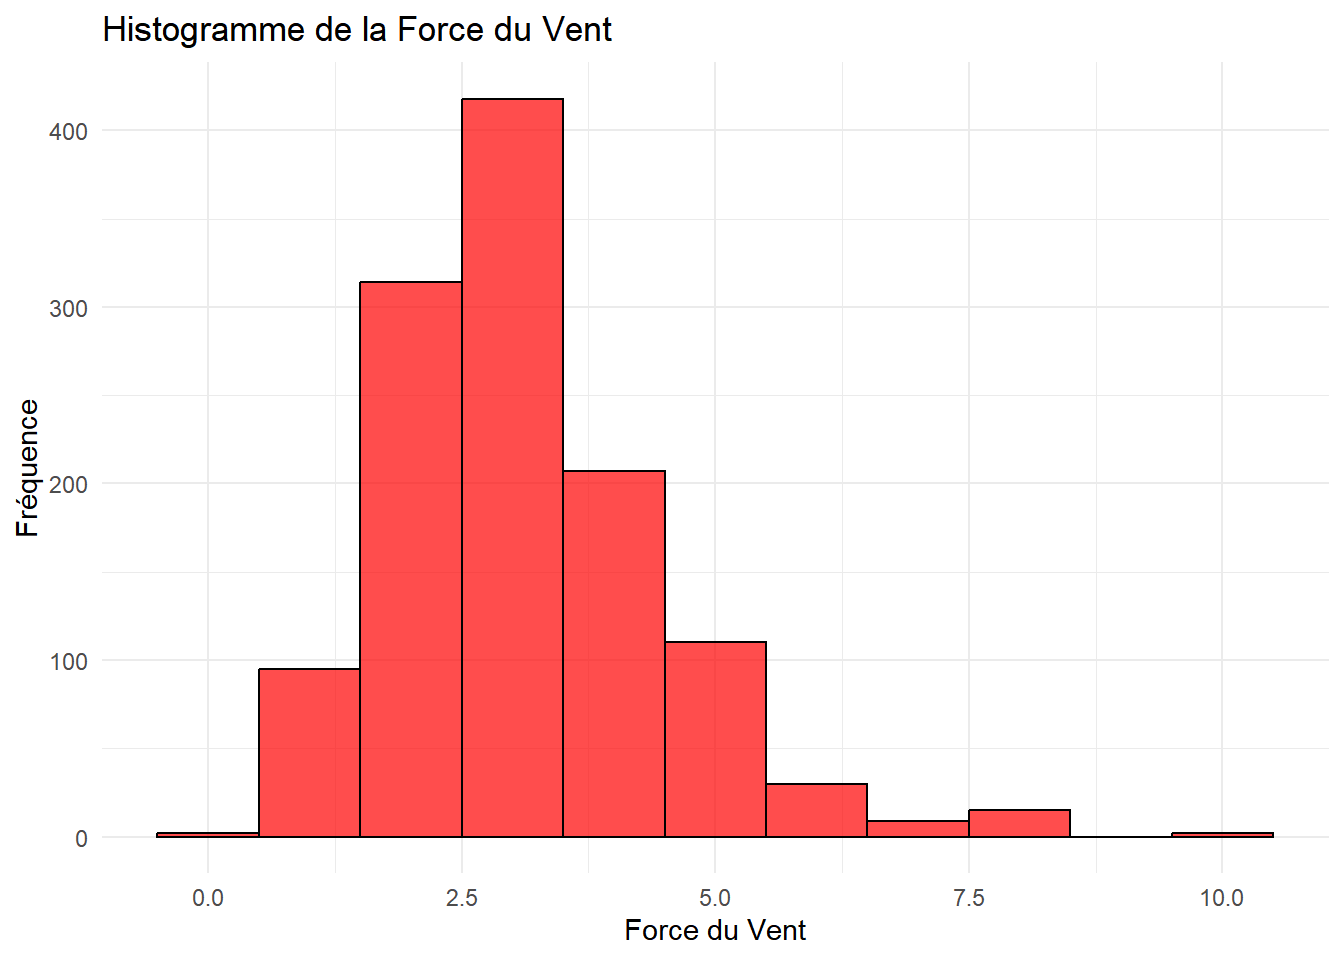
\includegraphics{Rapport_files/figure-latex/unnamed-chunk-8-1.pdf}

\textbf{Analyse Informatique:}

La variable ``année'' a été modifiée en un format numérique afin de
permettre son exploitation sans erreur dans les analyses à venir :

\textbf{incendies\(annee <- as.numeric(incendies\)annee)}

Les incendies dont la cause principale est répertoriée comme étant la
``malveillance'' ont pu être isolés grâce à la commande :

\textbf{incendies\_criminels \textless- subset(incendies,
nature\_inc\_prim == ``Malveillance'')}

Cela permet d'examiner plus en détail cette catégorie d'incendies.

La fonction table() a facilité le comptage des incendies criminels sur
une base annuelle. Ces résultats ont par la suite été convertis en
dataframe pour en faciliter une exploitation graphique ultérieure :

\textbf{incendies\_par\_annee\_df \textless- data.frame(annee =
as.numeric(names(incendies\_par\_annee)), nombre\_incendies =
as.vector(incendies\_par\_annee))}

Une tâche similaire a été réalisé pour tous les types d'incendies sans
exception :

\textbf{incendies\_total\_par\_annee\_df \textless- data.frame(annee =
as.numeric(names(incendies\_total\_par\_annee)),
nombre\_incendies\_total = as.vector(incendies\_total\_par\_annee))}

Cela facilitera la comparaison avec uniquement les incendies criminels.

Il sera désormais possible de produire des graphiques pour une
comparaison visuelle entre le nombre total d'incendies et celui des
incendies criminels.

Pour illustrer la comparaison entre les incendies criminels et le total
des incendies annuels, nous élaborons un diagramme où les points
symbolisant les incendies criminels sont reliés par une ligne de couleur
rouge.

Tous les points sont pris en compte par l'ajustement de l'axe Y.

Par la suite, nous incluons la courbe bleue représentant le total des
incendies, avec des points plus distincts.

Cela facilite l'identification des corrélations entre les pics
d'incendies criminels et les pics totaux.

Étant donné la difficulté de comparer les grandes valeurs du total sur
un seul axe Y, nous ajoutons un second axe à droite pour cette courbe.

Pour finir, nous positionnons la légende à la droite, en dehors du
diagramme, en désignant la ligne rouge comme représentant les incendies
criminels et la bleue comme le total.

Cette mesure rend les données présentées plus claires tout en préservant
une excellente lisibilité.

Ainsi, le graphique offre la possibilité d'analyser la corrélation entre
les incendies criminels et la progression générale des incendies au
cours des années.

\textbf{Analyse Statistique:}

Nous avons analysé le lien entre les incendies criminels intentionnels
et le total des incendies sur la période de 2012 à 2022.

L'axe des abscisses représente les différentes années tandis que l'axe
des ordonnées indique le nombre de feux.

On observe deux courbes :\\
- En \textbf{rouge}, l'évolution variable du nombre d'incendies
intentionnels (causés par la malveillance humaine).

\begin{itemize}
\tightlist
\item
  En \textbf{bleu}, le total variable des incendies relevés chaque
  année.
\end{itemize}

\textbf{Fluctuation du nombre total de feux :}

On observe une variation significative du total des incendies,
atteignant des pics en 2018 et 2022.

Ces augmentations pourraient être dues à des conditions climatiques
extrêmes ou à des phases prolongées de sécheresse qui favorisent les
incendies.

\textbf{Évolution des incendies criminels :}

Le nombre d'incendies criminels présente une tendance semblable, mais
avec une portée réduite.\\
Nous constatons une hausse marquée en 2022, qui pourrait signaler une
intensification des actes de malveillance intentionnelle.

\textbf{Corrélation partielle observée entre les deux graphiques :}

Bien que les incendies criminels suivent globalement la tendance
générale du nombre total de feux, quelques déviations demeurent.

Par exemple, en 2018, on observe une augmentation notable du total des
incendies, alors que la progression des feux d'origine criminelle reste
plus mesurée.

Ceci pourrait indiquer que d'autres éléments (météo, accidents) ont eu
un impact significatif sur l'augmentation générale des incendies cette
année-là.

L'étude indique que les incendies intentionnels constituent une part
importante de l'ensemble des feux, mais leur progression ne coïncide pas
toujours parfaitement avec la même tendance.

Les fluctuations des incendies pourraient être affectées par certains
phénomènes climatiques ou des phases de sécheresse prolongées, alors que
les feux allumés volontairement sont plus en lien avec des éléments
sociétaux et de sécurité.

Ces informations sont indispensables pour guider les stratégies de
prévention des incendies, en distinguant les actions à entreprendre en
fonction de la provenance des flammes.

\subparagraph{5.3.1.4 Analyse des incendies par mois et
saison}\label{analyse-des-incendies-par-mois-et-saison}

\begin{Shaded}
\begin{Highlighting}[]
\NormalTok{incendies }\OtherTok{\textless{}{-}} \FunctionTok{read.csv}\NormalTok{(}\StringTok{"../Data/donnees\_incendies.csv"}\NormalTok{)}
\NormalTok{incendies}\SpecialCharTok{$}\NormalTok{mois }\OtherTok{\textless{}{-}} \FunctionTok{factor}\NormalTok{(incendies}\SpecialCharTok{$}\NormalTok{mois, }\AttributeTok{levels =} \FunctionTok{c}\NormalTok{(}\StringTok{"Jan"}\NormalTok{, }\StringTok{"Feb"}\NormalTok{, }\StringTok{"Mar"}\NormalTok{, }\StringTok{"Apr"}\NormalTok{, }\StringTok{"May"}\NormalTok{, }\StringTok{"Jun"}\NormalTok{, }
                                                    \StringTok{"Jul"}\NormalTok{, }\StringTok{"Aug"}\NormalTok{, }\StringTok{"Sep"}\NormalTok{, }\StringTok{"Oct"}\NormalTok{, }\StringTok{"Nov"}\NormalTok{, }\StringTok{"Dec"}\NormalTok{))}

\NormalTok{nb\_incendies\_par\_mois }\OtherTok{\textless{}{-}} \FunctionTok{table}\NormalTok{(incendies}\SpecialCharTok{$}\NormalTok{mois)}

\FunctionTok{barplot}\NormalTok{(nb\_incendies\_par\_mois, }
        \AttributeTok{col =} \StringTok{"orange"}\NormalTok{, }
        \AttributeTok{border =} \StringTok{"black"}\NormalTok{, }
        \AttributeTok{main =} \StringTok{"Nombre d\textquotesingle{}incendies par mois"}\NormalTok{, }
        \AttributeTok{xlab =} \StringTok{"Mois"}\NormalTok{, }
        \AttributeTok{ylab =} \StringTok{"Nombre d\textquotesingle{}incendies"}\NormalTok{,}
        \AttributeTok{las =} \DecValTok{2}\NormalTok{)  }
\end{Highlighting}
\end{Shaded}

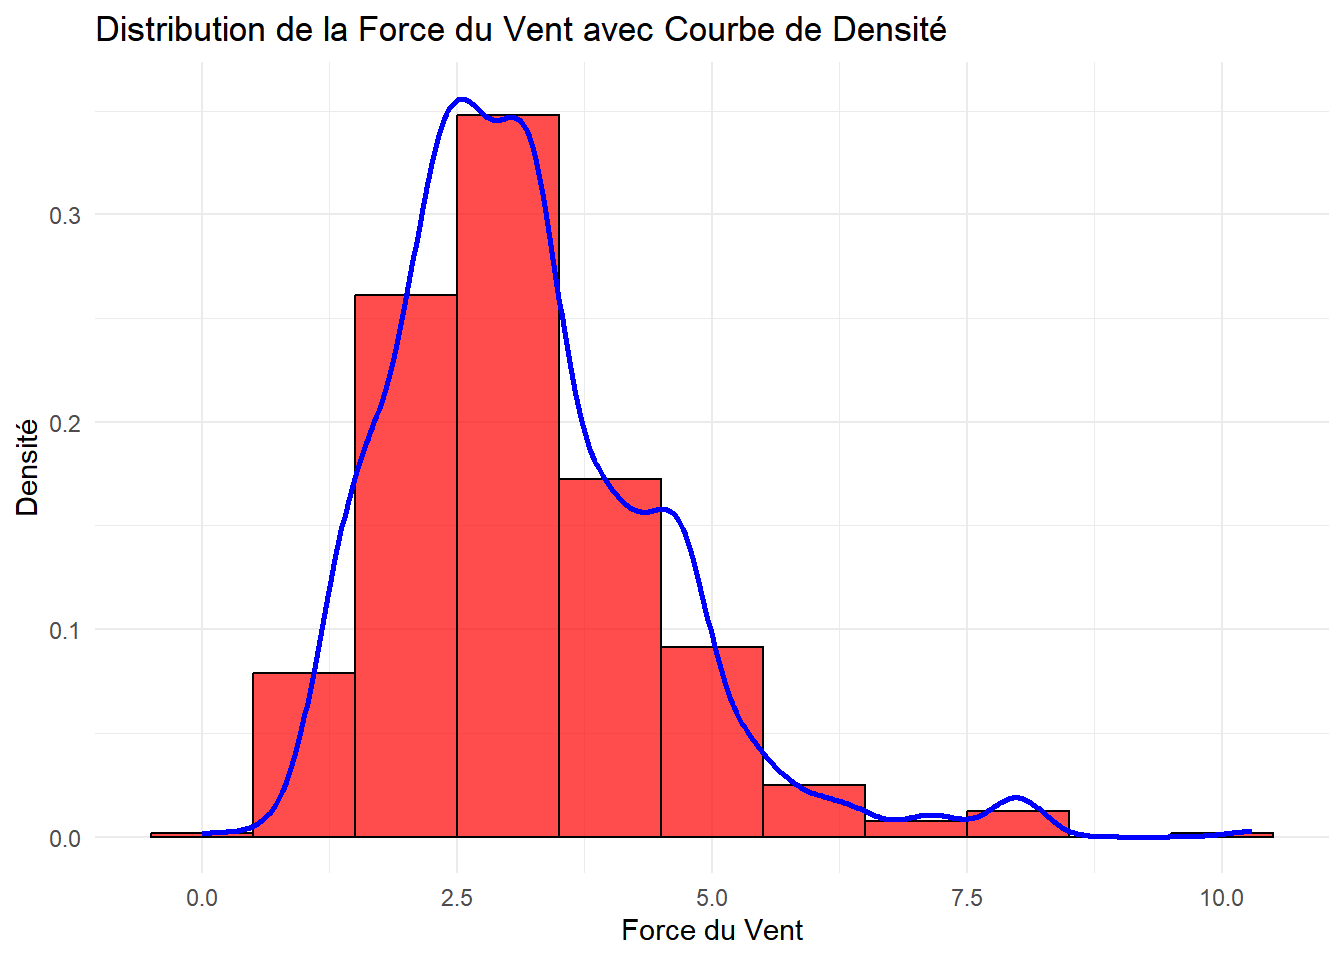
\includegraphics{Rapport_files/figure-latex/unnamed-chunk-9-1.pdf}

\begin{Shaded}
\begin{Highlighting}[]
\NormalTok{incendies}\SpecialCharTok{$}\NormalTok{saison }\OtherTok{\textless{}{-}} \ConstantTok{NA} 

\NormalTok{incendies}\SpecialCharTok{$}\NormalTok{saison[incendies}\SpecialCharTok{$}\NormalTok{mois }\SpecialCharTok{\%in\%} \FunctionTok{c}\NormalTok{(}\StringTok{"Dec"}\NormalTok{, }\StringTok{"Jan"}\NormalTok{, }\StringTok{"Feb"}\NormalTok{)] }\OtherTok{\textless{}{-}} \StringTok{"Hiver"}
\NormalTok{incendies}\SpecialCharTok{$}\NormalTok{saison[incendies}\SpecialCharTok{$}\NormalTok{mois }\SpecialCharTok{\%in\%} \FunctionTok{c}\NormalTok{(}\StringTok{"Mar"}\NormalTok{, }\StringTok{"Apr"}\NormalTok{, }\StringTok{"May"}\NormalTok{)] }\OtherTok{\textless{}{-}} \StringTok{"Printemps"}
\NormalTok{incendies}\SpecialCharTok{$}\NormalTok{saison[incendies}\SpecialCharTok{$}\NormalTok{mois }\SpecialCharTok{\%in\%} \FunctionTok{c}\NormalTok{(}\StringTok{"Jun"}\NormalTok{, }\StringTok{"Jul"}\NormalTok{, }\StringTok{"Aug"}\NormalTok{)] }\OtherTok{\textless{}{-}} \StringTok{"Été"}
\NormalTok{incendies}\SpecialCharTok{$}\NormalTok{saison[incendies}\SpecialCharTok{$}\NormalTok{mois }\SpecialCharTok{\%in\%} \FunctionTok{c}\NormalTok{(}\StringTok{"Sep"}\NormalTok{, }\StringTok{"Oct"}\NormalTok{, }\StringTok{"Nov"}\NormalTok{)] }\OtherTok{\textless{}{-}} \StringTok{"Automne"}

\NormalTok{nb\_incendies\_par\_saison }\OtherTok{\textless{}{-}} \FunctionTok{table}\NormalTok{(incendies}\SpecialCharTok{$}\NormalTok{saison)}

\NormalTok{couleurs\_saisons }\OtherTok{\textless{}{-}} \FunctionTok{c}\NormalTok{(}\StringTok{"Hiver"} \OtherTok{=} \StringTok{"blue"}\NormalTok{, }\StringTok{"Printemps"} \OtherTok{=} \StringTok{"green"}\NormalTok{, }\StringTok{"Été"} \OtherTok{=} \StringTok{"orange"}\NormalTok{, }\StringTok{"Automne"} \OtherTok{=} \StringTok{"brown"}\NormalTok{)}

\FunctionTok{barplot}\NormalTok{(nb\_incendies\_par\_saison, }
        \AttributeTok{col =}\NormalTok{ couleurs\_saisons[}\FunctionTok{names}\NormalTok{(nb\_incendies\_par\_saison)],  }
        \AttributeTok{border =} \StringTok{"black"}\NormalTok{, }
        \AttributeTok{main =} \StringTok{"Nombre d\textquotesingle{}incendies par saison"}\NormalTok{, }
        \AttributeTok{xlab =} \StringTok{"Saison"}\NormalTok{, }
        \AttributeTok{ylab =} \StringTok{"Nombre d\textquotesingle{}incendies"}\NormalTok{)}
\end{Highlighting}
\end{Shaded}

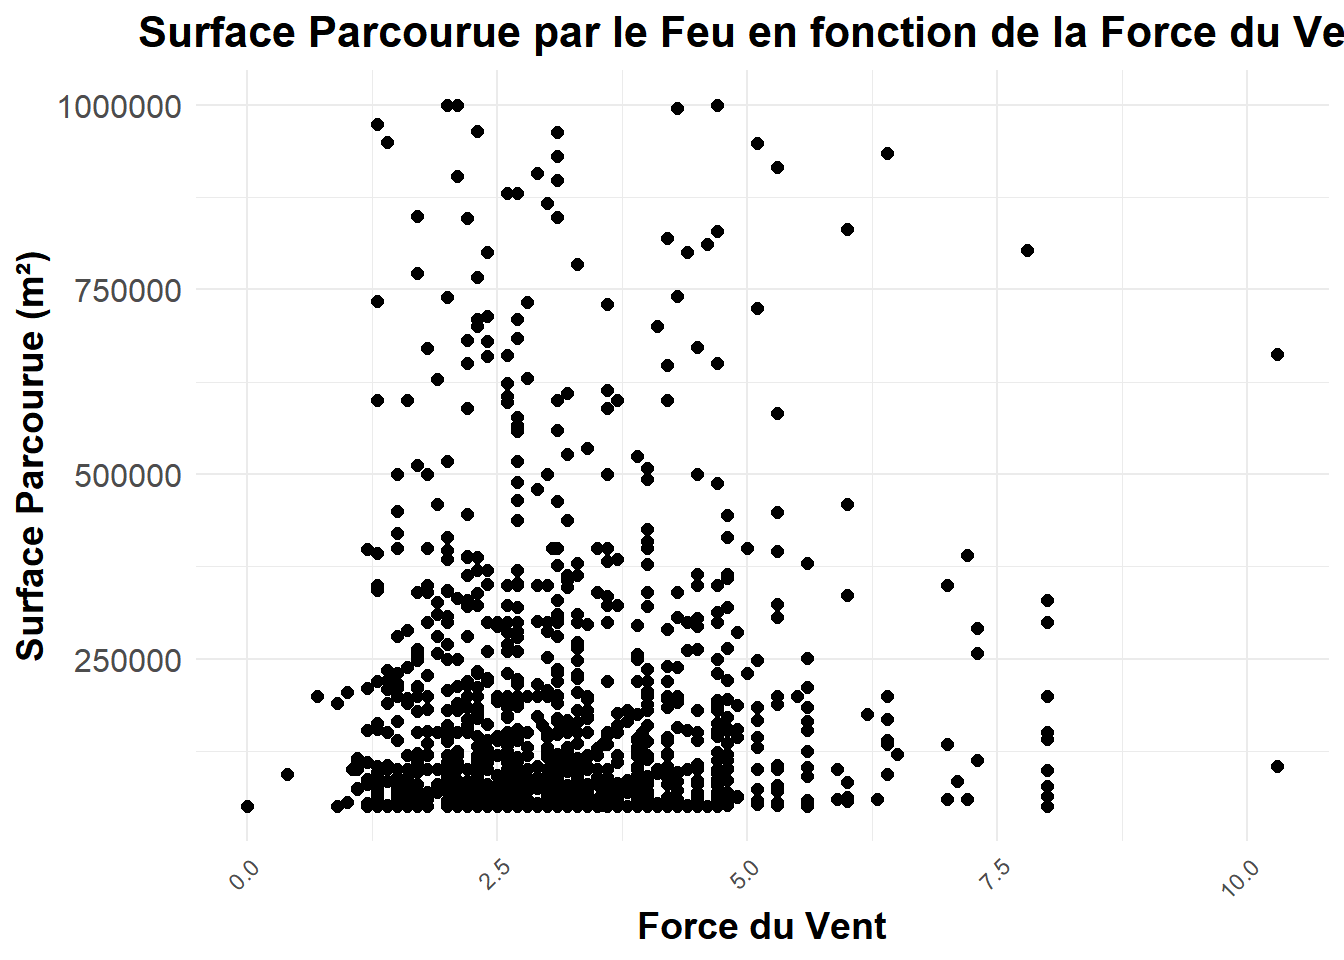
\includegraphics{Rapport_files/figure-latex/unnamed-chunk-10-1.pdf}

1- \textbf{Analyse Informatique:}

Pour débuter, nous arrangeons les mois selon l'ordre désiré :\\
\textbf{incendies\(mois <- factor(incendies\)mois, levels = c(``Jan'',
``Fév'', ``Mars'', ``Avr'', ``Mai'', ``Juin'', ``Juil'', ``Août'',
``Sept'', ``Oct'', ``Nov'', ``Décembre'')).}

Cette phase convertit la colonne mois en un facteur catégorique,
établissant clairement la séquence des mois de janvier à décembre.

Ceci assure un classement précis des mois lors de la création de
graphiques ou de calculs.

Ensuite, nous calculons le nombre d'incendies par mois avec la commande
\textbf{nb\_incendies\_par\_mois \textless- table(incendies\$mois)}.

Cette opération crée un tableau de décompte des incendies par mois.

Un diagramme à barres est donc généré pour représenter le nombre
d'incendies mensuels en utilisant
\textbf{barplot(nb\_incendies\_par\_mois,\ldots)}.

\textbf{Dans cette fonction :}

\begin{itemize}
\tightlist
\item
  \textbf{col=``orange''} : Les barres sont colorées en orange.
\item
  \textbf{border=``noir''} : Ajoute une bordure noire autour des barres.
\item
  **main=``Nombre** d'incendies par mois'' : Le titre du graphique.
\item
  \textbf{xlab=``Mois''} et \textbf{ylab=``Nombre d'incendies''} : Les
  étiquettes des axes.
\item
  **las=2* : Cette option fait pivoter les étiquettes des mois pour une
  meilleure lisibilité, surtout si les noms sont longs.
\end{itemize}

Par la suite, une colonne saison est ajoutée à l'objet incendie pour
assigner une saison à chaque mois.

L'instruction \textbf{incendies\$saison \textless- NA} initialise
d'abord une colonne vide, puis les lignes subséquentes attribuent une
saison à chaque mois en se basant sur les valeurs de la colonne mois :

\begin{itemize}
\tightlist
\item
  Déc, Jan, Fév : \textbf{Hiver}
\item
  Mars, Avr, Mai : \textbf{Printemps}
\item
  Juin, Juil, Août : \textbf{Été}
\item
  Sept, Oct, Nov : \textbf{Automne}
\end{itemize}

Après avoir analysé les données sur les incendies, nous avons calculé le
nombre d'incendies qui se sont produits pendant chaque saison à l'aide
de la fonction \textbf{table()}.

Cela nous a permis de générer un tableau croisé indiquant la fréquence
des incendies selon la période de l'année à laquelle ils se sont
déclarés.

2- \textbf{Analyse Statistique:}

Nous avons examiné le total d'incendies sur une durée de douze mois, de
janvier à décembre. L'axe horizontal indique les différents mois de
l'année, alors que l'axe vertical dépeint le nombre total d'incendies,
qui varie selon les périodes.

Le graphique illustre donc \textbf{les variations mensuelles}.

Pour visualiser facilement les variations, nous avons choisi \textbf{un
diagramme en barres}.

De \textbf{janvier à mars}, on observe une montée progressive du nombre
de feux, vraisemblablement due aux conditions hivernales qui accroissent
les dangers liés à la chaleur et l'usage des dispositifs de chauffage.

Cette évolution continue en \textbf{février et mars}.

En \textbf{mai}, le nombre d'incendies est relativement bas,
probablement à cause d'un temps plus clément et d'une diminution des
activités potentiellement dangereuses avant l'arrivée de l'été.

De \textbf{juin à août}, on observe une montée, surtout en juillet et
août, qui sont les mois les plus chauds où les activités humaines et
agricoles se multiplient, provoquant de nombreux incendies.

De \textbf{septembre à décembre}, les risques d'incendie diminuent
progressivement avec l'arrivée des mois plus frais et humides, réduisant
ainsi les dangers.

Cette répartition met en évidence l'influence du climat et des actes
humains en fonction des saisons, entre les besoins en chauffage d'hiver
et estivaux, augmentant ainsi les risques, à l'opposé de la période de
fin d'année.

Le \textbf{second graphique} propose une étude de la \textbf{récurrence
des feux en fonction des saisons sur le sol français.}

Les données sont distribuées selon les \textbf{quatre saisons
classiques} : l'hiver, le printemps, l'été et l'automne.

\textbf{L'axe horizontal} illustre ces diverses saisons alors que l'axe
vertical indique le total d'incendies pour chaque saison.

Pour représenter la distribution saisonnière des incendies, nous avons
choisi d'utiliser un diagramme à barres.

L'été se distingue de manière significative avec un nombre d'incendies
pratiquement triplé par rapport aux autres saisons.

Cela est dû aux températures élevées de l'été et à la hausse des dangers
d'incendies de forêt. Cette augmentation est également alimentée par
l'intensification des activités humaines pendant l'été, qu'il s'agisse
de la cultivation ou des divertissements en plein air.

Le nombre d'incendies au printemps est généralement inférieur mais plus
élevé qu'en automne et en hiver.

Ceci pourrait être dû à la fin de la saison hivernale combinée aux
premiers pics de chaleur, entraînant quelques incendies, en particulier
d'origine agricole.

Même si le nombre d'incendies à l'automne est moins élevé qu'en été, il
reste néanmoins important.

Des températures plus clémentes diminuent le danger des méga-incendies,
toutefois les travaux agricoles et la chute des feuilles continuent
d'être des éléments à risque.

L'hiver est marqué par une incidence réduite d'incendies grâce à des
températures basses et un taux d'humidité plus élevé qui minimisent les
dangers.

L'usage limité de certains appareils, tels que les cheminées, ainsi que
la réduction des activités en plein air contribuent aussi à ce nombre
réduit.

En définitive, l'analyse saisonnière des incendies met en évidence
l'impact du climat et des actions humaines sur leur occurrence.

L'été est la saison la plus risquée, tandis que l'hiver enregistre les
statistiques les plus faibles.

Ces informations sont indispensables aux services de prévention et
d'intervention pour identifier les saisons à haut risque et mettre en
place des dispositifs de sécurité appropriés.

Ainsi, le maximum de fréquence se produit durant l'été.

Il est probable que la médiane, c'est-à-dire la saison durant laquelle
50\% des incendies se produisent, se situe entre le printemps et l'été
étant donné la forte concentration estivale.

\subparagraph{5.3.1.5 Heures critiques de
déclenchement}\label{heures-critiques-de-duxe9clenchement}

\begin{Shaded}
\begin{Highlighting}[]
\CommentTok{\# 📦 Chargement des packages}
\FunctionTok{library}\NormalTok{(tidyverse)}
\FunctionTok{library}\NormalTok{(lubridate)}

\CommentTok{\# 📂 Charger les données}
\NormalTok{df }\OtherTok{\textless{}{-}} \FunctionTok{read\_csv}\NormalTok{(}\StringTok{"../Data/donnees\_incendies.csv"}\NormalTok{)}
\end{Highlighting}
\end{Shaded}

\begin{verbatim}
## Rows: 1202 Columns: 9
## -- Column specification --------------------------------------------------------
## Delimiter: ","
## chr (5): commune, code_INSEE, mois, nature_inc_prim, nature_inc_sec
## dbl (4): surface_parcourue_m2, annee, jour, heure
## 
## i Use `spec()` to retrieve the full column specification for this data.
## i Specify the column types or set `show_col_types = FALSE` to quiet this message.
\end{verbatim}

\begin{Shaded}
\begin{Highlighting}[]
\CommentTok{\# 🕒 Traitement des plages horaires}
\NormalTok{df }\OtherTok{\textless{}{-}}\NormalTok{ df }\SpecialCharTok{\%\textgreater{}\%}
  \FunctionTok{mutate}\NormalTok{(}
    \AttributeTok{heure\_num =} \FunctionTok{as.numeric}\NormalTok{(}\FunctionTok{str\_sub}\NormalTok{(heure, }\DecValTok{1}\NormalTok{, }\DecValTok{2}\NormalTok{)),  }\CommentTok{\# extrait l\textquotesingle{}heure (ex: "14:30" {-}\textgreater{} 14)}
    \AttributeTok{tranche\_horaire =} \FunctionTok{case\_when}\NormalTok{(}
\NormalTok{      heure\_num }\SpecialCharTok{\textgreater{}=} \DecValTok{0} \SpecialCharTok{\&}\NormalTok{ heure\_num }\SpecialCharTok{\textless{}} \DecValTok{3} \SpecialCharTok{\textasciitilde{}} \StringTok{"00{-}03h"}\NormalTok{,}
\NormalTok{      heure\_num }\SpecialCharTok{\textgreater{}=} \DecValTok{3} \SpecialCharTok{\&}\NormalTok{ heure\_num }\SpecialCharTok{\textless{}} \DecValTok{6} \SpecialCharTok{\textasciitilde{}} \StringTok{"03{-}06h"}\NormalTok{,}
\NormalTok{      heure\_num }\SpecialCharTok{\textgreater{}=} \DecValTok{6} \SpecialCharTok{\&}\NormalTok{ heure\_num }\SpecialCharTok{\textless{}} \DecValTok{9} \SpecialCharTok{\textasciitilde{}} \StringTok{"06{-}09h"}\NormalTok{,}
\NormalTok{      heure\_num }\SpecialCharTok{\textgreater{}=} \DecValTok{9} \SpecialCharTok{\&}\NormalTok{ heure\_num }\SpecialCharTok{\textless{}} \DecValTok{12} \SpecialCharTok{\textasciitilde{}} \StringTok{"09{-}12h"}\NormalTok{,}
\NormalTok{      heure\_num }\SpecialCharTok{\textgreater{}=} \DecValTok{12} \SpecialCharTok{\&}\NormalTok{ heure\_num }\SpecialCharTok{\textless{}} \DecValTok{15} \SpecialCharTok{\textasciitilde{}} \StringTok{"12{-}15h"}\NormalTok{,}
\NormalTok{      heure\_num }\SpecialCharTok{\textgreater{}=} \DecValTok{15} \SpecialCharTok{\&}\NormalTok{ heure\_num }\SpecialCharTok{\textless{}} \DecValTok{18} \SpecialCharTok{\textasciitilde{}} \StringTok{"15{-}18h"}\NormalTok{,}
\NormalTok{      heure\_num }\SpecialCharTok{\textgreater{}=} \DecValTok{18} \SpecialCharTok{\&}\NormalTok{ heure\_num }\SpecialCharTok{\textless{}} \DecValTok{21} \SpecialCharTok{\textasciitilde{}} \StringTok{"18{-}21h"}\NormalTok{,}
\NormalTok{      heure\_num }\SpecialCharTok{\textgreater{}=} \DecValTok{21} \SpecialCharTok{\&}\NormalTok{ heure\_num }\SpecialCharTok{\textless{}=} \DecValTok{23} \SpecialCharTok{\textasciitilde{}} \StringTok{"21{-}24h"}\NormalTok{,}
      \ConstantTok{TRUE} \SpecialCharTok{\textasciitilde{}} \StringTok{"Heure inconnue"}
\NormalTok{    )}
\NormalTok{  )}

\CommentTok{\# 📊 Comptage des incendies par tranche horaire et type}
\NormalTok{df\_summary }\OtherTok{\textless{}{-}}\NormalTok{ df }\SpecialCharTok{\%\textgreater{}\%}
  \FunctionTok{group\_by}\NormalTok{(tranche\_horaire, nature\_inc\_sec) }\SpecialCharTok{\%\textgreater{}\%}
  \FunctionTok{summarise}\NormalTok{(}\AttributeTok{n =} \FunctionTok{n}\NormalTok{(), }\AttributeTok{.groups =} \StringTok{"drop"}\NormalTok{)}

\CommentTok{\# 🧼 Re{-}niveautage pour un affichage logique des tranches}
\NormalTok{df\_summary}\SpecialCharTok{$}\NormalTok{tranche\_horaire }\OtherTok{\textless{}{-}} \FunctionTok{factor}\NormalTok{(}
\NormalTok{  df\_summary}\SpecialCharTok{$}\NormalTok{tranche\_horaire,}
  \AttributeTok{levels =} \FunctionTok{c}\NormalTok{(}\StringTok{"00{-}03h"}\NormalTok{, }\StringTok{"03{-}06h"}\NormalTok{, }\StringTok{"06{-}09h"}\NormalTok{, }\StringTok{"09{-}12h"}\NormalTok{, }\StringTok{"12{-}15h"}\NormalTok{, }\StringTok{"15{-}18h"}\NormalTok{, }\StringTok{"18{-}21h"}\NormalTok{, }\StringTok{"21{-}24h"}\NormalTok{)}
\NormalTok{)}

\CommentTok{\# 💅 Graphe stylisé (seul affiché)}
\FunctionTok{ggplot}\NormalTok{(df\_summary, }\FunctionTok{aes}\NormalTok{(}\AttributeTok{x =}\NormalTok{ tranche\_horaire, }\AttributeTok{y =}\NormalTok{ n, }\AttributeTok{fill =}\NormalTok{ nature\_inc\_sec)) }\SpecialCharTok{+}
  \FunctionTok{geom\_bar}\NormalTok{(}\AttributeTok{stat =} \StringTok{"identity"}\NormalTok{, }\AttributeTok{position =} \StringTok{"stack"}\NormalTok{, }\AttributeTok{width =} \FloatTok{0.7}\NormalTok{, }\AttributeTok{color =} \StringTok{"white"}\NormalTok{, }\AttributeTok{linewidth =} \FloatTok{0.3}\NormalTok{) }\SpecialCharTok{+}
  \FunctionTok{scale\_fill\_brewer}\NormalTok{(}\AttributeTok{palette =} \StringTok{"YlOrRd"}\NormalTok{) }\SpecialCharTok{+}
  \FunctionTok{labs}\NormalTok{(}
    \AttributeTok{title =} \StringTok{"🔥 Heures critiques des incendies par nature"}\NormalTok{,}
    \AttributeTok{subtitle =} \StringTok{"Répartition des incendies secondaires selon les tranches horaires"}\NormalTok{,}
    \AttributeTok{x =} \StringTok{"Tranche horaire"}\NormalTok{,}
    \AttributeTok{y =} \StringTok{"Nombre d\textquotesingle{}incendies"}\NormalTok{,}
    \AttributeTok{fill =} \StringTok{"Nature secondaire"}
\NormalTok{  ) }\SpecialCharTok{+}
  \FunctionTok{theme\_minimal}\NormalTok{(}\AttributeTok{base\_size =} \DecValTok{13}\NormalTok{) }\SpecialCharTok{+}
  \FunctionTok{theme}\NormalTok{(}
    \AttributeTok{plot.title =} \FunctionTok{element\_text}\NormalTok{(}\AttributeTok{face =} \StringTok{"bold"}\NormalTok{, }\AttributeTok{size =} \DecValTok{16}\NormalTok{, }\AttributeTok{color =} \StringTok{"\#B22222"}\NormalTok{),}
    \AttributeTok{plot.subtitle =} \FunctionTok{element\_text}\NormalTok{(}\AttributeTok{size =} \DecValTok{12}\NormalTok{, }\AttributeTok{margin =} \FunctionTok{margin}\NormalTok{(}\AttributeTok{b =} \DecValTok{10}\NormalTok{)),}
    \AttributeTok{axis.text.x =} \FunctionTok{element\_text}\NormalTok{(}\AttributeTok{angle =} \DecValTok{45}\NormalTok{, }\AttributeTok{hjust =} \DecValTok{1}\NormalTok{),}
    \AttributeTok{legend.position =} \StringTok{"right"}\NormalTok{,}
    \AttributeTok{legend.background =} \FunctionTok{element\_rect}\NormalTok{(}\AttributeTok{fill =} \StringTok{"transparent"}\NormalTok{),}
    \AttributeTok{panel.grid.major.y =} \FunctionTok{element\_line}\NormalTok{(}\AttributeTok{color =} \StringTok{"\#eeeeee"}\NormalTok{),}
    \AttributeTok{panel.grid.minor =} \FunctionTok{element\_blank}\NormalTok{()}
\NormalTok{  )}
\end{Highlighting}
\end{Shaded}

\includegraphics{Rapport_files/figure-latex/unnamed-chunk-11-1.pdf}

\begin{enumerate}
\def\labelenumi{\arabic{enumi}.}
\tightlist
\item
  \textbf{Analyse Informatique}
\end{enumerate}

Initialement, on importe les données à partir d'un fichier externe au
format CSV en utilisant la fonction \textbf{read\_csv()}, qui assure une
performance maximale pour de grandes quantités de données organisées en
tableau.

Cette importation présuppose la présence et une bonne structuration des
champs clés, notamment l'heure à laquelle chaque incendie a eu lieu
(heure) et son type secondaire (nature\_inc\_sec).

Le but est de combiner ces deux aspects afin d'identifier des schémas
temporels de déclenchement, c'est-à-dire des créneaux horaires plus
susceptibles d'être liés au démarrage d'incendies de divers types.

L'analyse temporelle des données s'effectue en utilisant une
segmentation basée sur des intervalles horaires fixes, divisés ici par
tranches de trois heures : de minuit à 03h, de 03h à 06h, et ainsi de
suite jusqu'à 21h-24h.

La conversion des heures brutes en segments horaires classés se fait par
l'intermédiaire de la fonction mutate() du tidyverse, associée à une
condition case\_when().

Cette méthode garantit un traitement vectorisé et cohérent de la colonne
heure.

Après avoir déterminé les créneaux horaires, les données sont regroupées
en combinant les variables tranche\_horaire et nature\_inc\_sec.~

Cela donne lieu à un tableau de contingence dénormalisé, qui montre le
nombre d'incendies qui se sont produits dans chaque plage horaire pour
chaque type secondaire d'incendie.

Ce regroupement est réalisé en utilisant les fonctions group\_by() et
summarise(), conformément aux normes de manipulation de données en
pipeline caractéristiques du paradigme tidyverse.

Cette compilation sert de fondement à l'analyse visuelle subséquente.

La visualisation s'appuie sur le package ggplot2, très apprécié pour sa
flexibilité et sa performance dans l'illustration graphique de données
complexes.

On propose deux variantes du diagramme : une première d'origine, qui
utilise une palette viridis conçue pour l'accessibilité (en particulier
pour les personnes atteintes de daltonisme), et une seconde, plus
esthétique et sémantique, tirée de la palette YlOrRd dérivée de
RColorBrewer.

Cette palette de couleurs, variant du jaune clair au rouge profond,
évoque instinctivement la puissance et la chaleur du feu, ce qui apporte
une cohérence visuelle en rapport avec le phénomène analysé.

Le mode empilé de geom\_bar() est utilisé pour visualiser à la fois le
volume total d'incendies par segment horaire et leur répartition interne
selon les types secondaires.

L'incorporation d'aspects esthétiques --- comme l'inclinaison des labels
de l'axe X, le style typographique du titre, l'épaisseur des barres ou
même la présence d'un fond blanc autour des segments --- témoigne d'une
préoccupation marquée pour la clarté du graphique.

Ces sélections respectent les meilleures méthodes en visualisation
scientifique, où la transparence de l'information prévaut sur l'impact
esthétique brut.

En outre, l'utilisation de factor() pour la classification manuelle de
la variable tranche\_horaire assure un classement basé sur l'ordre
logique plutôt que sur l'ordre alphabétique des tranches, prévenant
ainsi toute confusion dans l'analyse temporelle.

\begin{enumerate}
\def\labelenumi{\arabic{enumi}.}
\setcounter{enumi}{1}
\tightlist
\item
  \textbf{Analyse Statistique:}
\end{enumerate}

Le diagramme désigné « Heures critiques des incendies par nature :
Distribution des incendies secondaires selon les créneaux horaires »
offre une représentation graphique des informations relatives à la
périodicité des incendies secondaires en lien avec les tranches horaires
sur une durée de 24 heures. On distingue deux types majeurs d'incendies
secondaires : « particulier » et « travaux », auxquels s'ajoute une
catégorie supplémentaire « NA » (non attribuée).

L'axe horizontal illustre les intervalles de temps (de 00h-03h à
21h-24h), alors que l'axe vertical dépeint le nombre d'incendies, avec
une gamme s'étendant de 0 à 450.

Cette étude a pour objectif d'explorer la répartition temporelle des
incendies secondaires, de déterminer les moments clés, et d'aborder
l'importance de ces conclusions dans une perspective statistique et
pratique.

Le diagramme est un histogramme superposé, où chaque colonne illustre un
segment horaire de trois heures. Les segments colorés sur les barres
sont : un jaune pâle pour les incendies dits « particuliers », l'orange
pour ceux liés aux « travaux », et une ligne noire mince pour la
catégorie « NA ».

Une première analyse montre une grande fluctuation du nombre d'incendies
en fonction des créneaux horaires. Les créneaux horaires de 15h à 18h et
de 18h à 21h montrent les taux les plus élevés, avoisinant les 400
incendies, alors que les plages horaires de minuit à 3h, de 3h à 6h et
de 21h à minuit dénotent des fréquences très basses, en dessous de 50
incendies.

Concernant la répartition par nature, les incendies classés comme «
particulier » et « travaux » prédominent de manière significative,
tandis que la catégorie « NA » a une contribution négligeable. Il semble
que les incendies associés aux « travaux » soient un peu plus courants
que ceux classés comme « particulier » durant les périodes de forte
activité (15h-18h et 18h-21h), ce qui indique une éventuelle relation
entre les activités professionnelles et l'apparition de ces incendies
secondaires.

\begin{itemize}
\tightlist
\item
  00h-03h : \textasciitilde10 incendies (majoritairement ``travaux'',
  faible contribution ``NA'').
\item
  03h-06h : \textasciitilde20 incendies (similaire à la tranche
  précédente, avec une légère augmentation des ``particuliers'').
\item
  06h-09h : \textasciitilde20 incendies (répartition équilibrée entre
  ``particulier'' et ``travaux'').
\item
  09h-12h : \textasciitilde120 incendies (augmentation notable, avec une
  répartition \textasciitilde50/50 entre ``particulier'' et
  ``travaux'').
\item
  12h-15h : \textasciitilde100 incendies (légère baisse par rapport à la
  tranche précédente, répartition similaire).
\item
  15h-18h : \textasciitilde400 incendies (pic maximal, avec
  \textasciitilde200 ``particulier'' et \textasciitilde200 ``travaux'').
\item
  18h-21h : \textasciitilde380 incendies (second pic, répartition
  similaire à 15h-18h).
\item
  21h-24h : \textasciitilde50 incendies (forte baisse, avec une
  contribution mineure de ``NA'').
\end{itemize}

Il est évident que les créneaux horaires de 15h à 18h et de 18h à 21h
sont les plus critiques, car ils constituent près de 80 \% du nombre
total d'incendies secondaires sur une journée (en supposant un total
approximatif de 1000 incendies sur 24 heures, estimation fondée sur la
hauteur cumulative des barres).

Cette focalisation temporelle indique un phénomène de nature cyclique
associé à des éléments humains ou environnementaux, que nous examinerons
plus en détail par la suite.

L'analyse de la répartition entre les catégories « particulier » et «
travaux » révèle une symétrie notable durant les plages horaires les
plus dynamiques.

Par exemple, dans la plage horaire de 15h à 18h, les deux catégories
contribuent presque de manière équivalente (\textasciitilde200 incendies
pour chacune).

Cela pourrait suggérer que les incendies secondaires, qu'ils soient
d'origine domestique (« particulier ») ou professionnelle (« travaux »),
ont en commun certains facteurs déclenchants à ces moments précis, tels
qu'une intensification de l'activité humaine, une augmentation de la
température, ou des conditions environnementales particulières (vent,
sécheresse).

La catégorie « NA » demeure marginale, ne représentant jamais plus de 5
\% du total à aucun moment de la journée.

Cela indique une classification efficace des données, avec peu
d'incidents non attribués.

Toutefois, cette catégorie pourrait mettre en évidence des insuffisances
dans la collecte de données ou des incendies dont l'origine reste
inconnue, ce qui nécessite une considération spécifique dans une analyse
plus détaillée.

Pour structurer l'étude, envisageons la distribution des incendies comme
une série temporelle discrète sur 24 heures, segmentée en 8 tranches de
3 heures.

On remarque une distribution fortement asymétrique, avec un regroupement
notable entre 15h et 21h.

Les créneaux horaires de pointe identifiés (15h-21h) correspondent à des
moments d'intense activité humaine.

Concernant les incendies de catégorie « travaux », ceux-ci peuvent
correspondre à des opérations professionnelles ou industrielles qui
atteignent leur point culminant en fin de journée, tels que des projets
de construction ou d'entretien nécessitant l'utilisation d'équipements
dangereux (soudure, machines électriques).

En ce qui concerne les incendies dits « particuliers », cette tranche
horaire pourrait coïncider avec des activités domestiques telles que la
préparation des repas ou l'usage d'appareils électroménagers, qui ont
généralement tendance à se produire plus régulièrement en fin de
journée.

Des éléments environnementaux, comme la température ou l'humidité,
pourraient aussi avoir une influence, particulièrement si les
informations se rapportent à une saison de l'année sujette aux feux
(été). Il est probable que la diminution de l'activité humaine durant la
nuit et tôt le matin soit à l'origine des basses fréquences observées
entre minuit et 9h.

En résumé, l'examen statistique du diagramme montre une importante
concentration d'incendies secondaires entre 15h et 21h, avec une
distribution équilibrée entre les catégories « particulier » et «
travaux ».

\subparagraph{5.3.1.6 Cyclicité
hebdomadaire}\label{cyclicituxe9-hebdomadaire}

\begin{Shaded}
\begin{Highlighting}[]
\NormalTok{incendies }\OtherTok{\textless{}{-}} \FunctionTok{read.csv}\NormalTok{(}\StringTok{"../Data/donnees\_incendies.csv"}\NormalTok{)}

\NormalTok{incendies}\SpecialCharTok{$}\NormalTok{jour }\OtherTok{\textless{}{-}} \FunctionTok{as.Date}\NormalTok{(incendies}\SpecialCharTok{$}\NormalTok{jour, }\AttributeTok{format=}\StringTok{"\%Y{-}\%m{-}\%d"}\NormalTok{)}

\FunctionTok{head}\NormalTok{(incendies}\SpecialCharTok{$}\NormalTok{jour)}
\end{Highlighting}
\end{Shaded}

\begin{verbatim}
## [1] "1970-01-29" "1970-01-30" "1970-01-03" "1970-01-03" "1970-01-09"
## [6] "1970-01-15"
\end{verbatim}

\begin{Shaded}
\begin{Highlighting}[]
\FunctionTok{Sys.setlocale}\NormalTok{(}\StringTok{"LC\_TIME"}\NormalTok{, }\StringTok{"fr\_FR.UTF{-}8"}\NormalTok{)  }
\end{Highlighting}
\end{Shaded}

\begin{verbatim}
## [1] "fr_FR.UTF-8"
\end{verbatim}

\begin{Shaded}
\begin{Highlighting}[]
\NormalTok{incendies}\SpecialCharTok{$}\NormalTok{jour\_semaine }\OtherTok{\textless{}{-}} \FunctionTok{weekdays}\NormalTok{(incendies}\SpecialCharTok{$}\NormalTok{jour, }\AttributeTok{abbreviate =} \ConstantTok{FALSE}\NormalTok{)}

\FunctionTok{print}\NormalTok{(}\FunctionTok{unique}\NormalTok{(incendies}\SpecialCharTok{$}\NormalTok{jour\_semaine)) }
\end{Highlighting}
\end{Shaded}

\begin{verbatim}
## [1] "jeudi"    "vendredi" "samedi"   "dimanche" "mercredi" "mardi"    "lundi"
\end{verbatim}

\begin{Shaded}
\begin{Highlighting}[]
\NormalTok{incendies}\SpecialCharTok{$}\NormalTok{jour\_semaine }\OtherTok{\textless{}{-}} \FunctionTok{factor}\NormalTok{(incendies}\SpecialCharTok{$}\NormalTok{jour\_semaine, }
                                 \AttributeTok{levels =} \FunctionTok{c}\NormalTok{(}\StringTok{"lundi"}\NormalTok{, }\StringTok{"mardi"}\NormalTok{, }\StringTok{"mercredi"}\NormalTok{, }\StringTok{"jeudi"}\NormalTok{, }\StringTok{"vendredi"}\NormalTok{, }\StringTok{"samedi"}\NormalTok{, }\StringTok{"dimanche"}\NormalTok{))}

\NormalTok{semaine\_incendies }\OtherTok{\textless{}{-}} \FunctionTok{sum}\NormalTok{(incendies}\SpecialCharTok{$}\NormalTok{jour\_semaine }\SpecialCharTok{\%in\%} \FunctionTok{c}\NormalTok{(}\StringTok{"lundi"}\NormalTok{, }\StringTok{"mardi"}\NormalTok{, }\StringTok{"mercredi"}\NormalTok{, }\StringTok{"jeudi"}\NormalTok{, }\StringTok{"vendredi"}\NormalTok{))}
\NormalTok{weekend\_incendies }\OtherTok{\textless{}{-}} \FunctionTok{sum}\NormalTok{(incendies}\SpecialCharTok{$}\NormalTok{jour\_semaine }\SpecialCharTok{\%in\%} \FunctionTok{c}\NormalTok{(}\StringTok{"samedi"}\NormalTok{, }\StringTok{"dimanche"}\NormalTok{))}

\NormalTok{total\_incendies }\OtherTok{\textless{}{-}} \FunctionTok{c}\NormalTok{(}\AttributeTok{semaine =}\NormalTok{ semaine\_incendies, }\AttributeTok{weekend =}\NormalTok{ weekend\_incendies)}

\FunctionTok{par}\NormalTok{(}\AttributeTok{mar =} \FunctionTok{c}\NormalTok{(}\DecValTok{2}\NormalTok{, }\DecValTok{2}\NormalTok{, }\DecValTok{2}\NormalTok{, }\DecValTok{2}\NormalTok{))  }
\FunctionTok{pie}\NormalTok{(total\_incendies, }
    \AttributeTok{col =} \FunctionTok{c}\NormalTok{(}\StringTok{"lightblue"}\NormalTok{, }\StringTok{"orange"}\NormalTok{), }
    \AttributeTok{main =} \StringTok{"Repartition des incendies entre semaine et week{-}end"}\NormalTok{,}
    \AttributeTok{labels =} \FunctionTok{c}\NormalTok{(}\StringTok{"Semaine (Lun{-}Ven)"}\NormalTok{, }\StringTok{"Week{-}end (Sam{-}Dim)"}\NormalTok{),}
    \AttributeTok{cex =} \DecValTok{1}\NormalTok{) }
\end{Highlighting}
\end{Shaded}

\includegraphics{Rapport_files/figure-latex/unnamed-chunk-12-1.pdf}

\begin{enumerate}
\def\labelenumi{\arabic{enumi}.}
\tightlist
\item
  \textbf{Analyse Informatique:}
\end{enumerate}

\textbf{Transformation de la colonne ``date'' en type Date:}

Nous utilisons la fonction as.Date() pour transformer la colonne « date
» en un objet de type Date. Le format indiqué est
\textbf{``\%Y-\%m-\%d''}, qui représente \textbf{l'année, le mois et le
jour selon la norme}.

\textbf{Extraction du jour de la semaine:}

La fonction \textbf{weekdays()} est employée pour extraire \textbf{le
nom du jour de la semaine} à partir de la colonne \textbf{date}.

Nous commençons par définir la langue française de localisation grâce à
\textbf{Sys.setlocale()}, afin que les jours soient affichés dans cette
langue, comme par exemple « lundi ».

\textbf{Verification des jours uniques:}

Cette instruction permet de montrer les valeurs distinctes trouvées dans
la colonne « jour\_semaine » pour vérifier les jours récupérés.

\textbf{Création d'un facteur pour les jours:}

Nous convertissons la colonne « jour\_semaine » en facteur, avec les
niveaux des jours clairement définis de lundi à dimanche, assurant ainsi
leur séquence correcte.

\textbf{Calcul du nombre d'incendies pendant la semaine et le weekend:}

Nous comptons ici les incendies qui se déclenchent durant \textbf{la
semaine, du lundi au vendredi}, ainsi que pendant \textbf{le week-end},
c'est-à-dire \textbf{samedi et dimanche}.

Ceci est effectué en utilisant l'opérateur \textbf{\%in\%} pour
confirmer quel jour correspond à l'événement.

\textbf{Création d'un vecteur avec les résultats:}

Un tableau nommé \textbf{« total\_incendies »} est créé pour conserver
\textbf{les résultats} des incendies durant la \textbf{semaine et le
week-end}.

\textbf{Creation d'un graphique circulaire:}

Pour finir, nous utilisons la fonction \textbf{pie()} pour créer un
\textbf{diagramme circulaire} afin d'illustrer la répartition des
incendies entre la semaine et le weekend, en optant pour des couleurs et
étiquettes sur mesure, tout en modifiant les marges pour une
présentation plus soignée.

\begin{enumerate}
\def\labelenumi{\arabic{enumi}.}
\setcounter{enumi}{1}
\tightlist
\item
  \textbf{Analyse Statistique:}
\end{enumerate}

\textbf{Incendies fréquents pendant la semaine active:}

Les informations indiquent que la majorité des incendies se déclarent en
semaine, à cause de divers facteurs.

Parfois, l'augmentation de l'activité humaine et une forte densité de
population peuvent engendrer plus de risques.

Au cours des heures de travail et durant les déplacements, les activités
domestiques ou industrielles augmentent les risques potentiels.

De plus, les incendies peuvent également être favorisés par le travail
ou les conditions météorologiques : l'usage d'instruments ou
d'équipements électriques lors de journées de travail intenses en est
fréquemment une raison.

\textbf{Fin de semaine plus paisible:}

Le week-end semble présenter un risque d'incendie réduit, en raison de
la diminution des activités professionnelles et industrielles, ainsi que
de la réduction des déplacements et de l'utilisation d'appareils
susceptibles de déclencher un feu.

Il est probable qu'en week-end, lorsque les activités commerciales et
industrielles sont réduites ou absentes, les personnes utilisent moins
d'appareils ou adoptent davantage de mesures de précaution.

\paragraph{5.3.2 Facteurs climatiques et
météorologiques}\label{facteurs-climatiques-et-muxe9tuxe9orologiques}

\subparagraph{5.3.2.1 Influence de la température sur les
incendies}\label{influence-de-la-tempuxe9rature-sur-les-incendies}

\subparagraph{5.3.2.2 Impact de l'humidité sur les
incendies}\label{impact-de-lhumidituxe9-sur-les-incendies}

Pour mener l'analyse de l'influence de l'humidité sur les incendies, il
est nécessaire de constituer notre base d'analyse. Il est nécessaire
d'utiliser les deux tables que nous avons mises en place dans notre Base
de données, à savoir la Table Incendies et la Table donnees\_meteo.

Afin de réaliser une jointure entre ces deux tables, nous avons fait
appel à une troisième table nommée humidite qui regroupe les champs des
deux tables visées, partageant un élément en commun : le « Code\_INSEE
». Nous avons détaillé la méthode utilisée pour cela dans la section
Informatique de notre rapport.

Avant d'approfondir dans les détails de notre étude, nous allons d'abord
définir les termes clés que nous utiliserons dans notre analyse.
L'humidité se réfère à la présence de vapeur d'eau dans l'air.

Le but de notre analyse est d'étudier le lien entre l'humidité
atmosphérique et les incendies. Pour accomplir cela, nous devons étudier
la relation entre l'humidité et la dimension des incendies.

\emph{Il est essentiel de mettre en évidence deux attributs importants.}

\begin{enumerate}
\def\labelenumi{\arabic{enumi}.}
\item
  \textbf{Tens\_vap\_med}: Cet attribut évalue la pression de
  vaporisation moyenne, qui est une autre façon de dire qu'il s'agit
  d'un indicateur de l'humidité de l'air.
\item
  \textbf{surface\_parcourue\_m2}: Cette caractéristique présente la
  superficie ravagée par un feu, ce qui en fait un instrument pour
  évaluer l'intensité du feu.
\end{enumerate}

Dans cette étude, nous allons créer et analyser deux graphes
indispensables à notre problématique.

\begin{enumerate}
\def\labelenumi{\arabic{enumi}.}
\tightlist
\item
  \textbf{Histogramme de l'humidité}
\end{enumerate}

Le diagramme de l'humidité nous aidera à examiner et à saisir la
distribution des taux d'humidité dans l'échantillon de données.

L'humidité joue un rôle crucial dans l'analyse des incendies en raison
de son impact sur la rapidité de leur avancement. Cependant, avant
d'examiner toute relation avec la surface incendiée, nous devons d'abord
comprendre comment l'humidité fluctue dans les données.

\begin{Shaded}
\begin{Highlighting}[]
\FunctionTok{library}\NormalTok{(ggplot2)}
\NormalTok{data }\OtherTok{\textless{}{-}} \FunctionTok{read.csv}\NormalTok{(}\StringTok{"../Exports/export\_Humidites.csv"}\NormalTok{)}
\FunctionTok{ggplot}\NormalTok{(data, }\FunctionTok{aes}\NormalTok{(}\AttributeTok{x =}\NormalTok{ Tens\_vap\_med)) }\SpecialCharTok{+}
  \FunctionTok{geom\_histogram}\NormalTok{(}\AttributeTok{binwidth =} \FloatTok{0.5}\NormalTok{, }\AttributeTok{fill =} \StringTok{"\#1f77b4"}\NormalTok{, }\AttributeTok{color =} \StringTok{"white"}\NormalTok{, }\AttributeTok{alpha =} \FloatTok{0.7}\NormalTok{) }\SpecialCharTok{+}
  \FunctionTok{labs}\NormalTok{(}\AttributeTok{title =} \StringTok{"Distribution de l\textquotesingle{}humidité de l\textquotesingle{}air (Tens\_vap\_med)"}\NormalTok{, }
       \AttributeTok{x =} \StringTok{"Humidité de l\textquotesingle{}air (Tens\_vap\_med)"}\NormalTok{, }
       \AttributeTok{y =} \StringTok{"Fréquence"}\NormalTok{) }\SpecialCharTok{+}
  \FunctionTok{theme\_minimal}\NormalTok{()}
\end{Highlighting}
\end{Shaded}

\includegraphics{Rapport_files/figure-latex/unnamed-chunk-13-1.pdf}

\begin{enumerate}
\def\labelenumi{\arabic{enumi}.}
\tightlist
\item
  \textbf{Analyse Informatique:}
\end{enumerate}

Dans notre code destiné à la création du graphique, nous avons employé
le langage R pour sa réalisation. Tout d'abord, nous avons importé le
fichier en utilisant la méthode \textbf{read.csv()}.

Par la suite, on procède à l'initialisation du graphique que l'on
souhaite concevoir avec la méthode \textbf{ggplot()}.On passe en
paramètres de cette méthode les données ainsi que l'\textbf{aes},qui
nous permet de spécifier que l'axe des x sera représenté par
\textbf{Tens\_vap\_med}.

On définit ensuite une autre méthode \textbf{geom\_histogram()} pour
intégrer un histogramme au graphique. Dans cette méthode, on spécifie
des paramètres pour déterminer la largeur des barres de l'histogramme,
et par la suite, on remplit les barres en bleu. Nous définissons la
bordure en blanc et rendons les barres davantage transparentes.

On détermine les titres et étiquettes en faisant appel à la méthode
\textbf{labs()}, en exploitant les paramètres title, x et y.Le titre
indique le sujet du graphique, `x' correspond à l'étiquette de l'axe
horizontal et `y' correspond à l'étiquette de l'axe vertical.

Et pour donner un aspect minimaliste au thème, nous avons employé la
méthode \textbf{theme\_minimal()} afin d'incorporer un style plus
contemporain.

\begin{enumerate}
\def\labelenumi{\arabic{enumi}.}
\setcounter{enumi}{1}
\tightlist
\item
  \textbf{Analyse Statistique:}
\end{enumerate}

L'axe des abscisses illustre l'humidité de l'air, déterminée par la
pression de vapeur moyenne. Les chiffres se situent approximativement
entre 0 et 25.On présume que les valeurs sont exprimées en hPa. C'est
une unité utilisée pour évaluer la pression de la vapeur.

L'axe ordonnes illustre la fréquence, c'est-à-dire le total des
observations pour chaque plage de tension de vapeur. Il a atteint une
fréquence maximale de 200.

D'après les informations intégrées, cet histogramme révèle une
distribution asymétrique avec une importante concentration de valeurs
faibles en matière d'humidité de l'air, allant de 5 à 15 hPa.

L'histogramme présente une asymétrie vers la droite, avec un grand
nombre d'observations ayant de faibles valeurs de tension de vapeur,
indiquant une humidité faible à modérée, et quelques observations à des
valeurs plus élevées, traduisant une humidité supérieure.

On pourrait affirmer que la classe modale de cet histogramme se situe
approximativement entre 10 et 12 hPa.

La portée de cet histogramme s'étend de 0 à 25 hPa. Néanmoins, on
remarque qu'il existe très peu de données entre 20 et 25 hPa. De plus,
il est évident qu'au-delà de 22 hPa, aucune observation n'est présente.

Dans notre histogramme, on peut observer la présence d'une longue queue,
bien qu'elle soit peu dense. Autrement dit, cela nous indique que les
valeurs élevées de tension de vapeur sont peu fréquentes dans cet
ensemble de données.

Nous allons déterminer les interprétations des intervalles concernant le
taux d'humidité.

\begin{enumerate}
\def\labelenumi{\arabic{enumi}.}
\tightlist
\item
  \textbf{0 a 5 hPa}: Cette plage indique un taux d'humidité très bas.
\item
  \textbf{5 a 15 hPa}: C'est la zone où est rassemblée la plupart des
  données. La fréquence s'accroît rapidement dès que l'on atteint 5 hPa,
  atteignant un maximum aux alentours de 10 à 12 hPa avant de
  redescendre. Cela signifie que le niveau d'humidité est modéré.
\item
  \textbf{15 a 20 hPa}:Dans cette période, nous observons une réduction
  qui est associée à des conditions plus humides.
\item
  \textbf{20 a 25 hPa}:Les observations sont peu fréquentes. La
  fréquence étant pratiquement de 0, on peut observer que nous avons des
  conditions hors du commun, telles que des climats tropicaux.
\end{enumerate}

Dans un cadre météorologique, la tension de vapeur représente une
évaluation de la pression partielle de la vapeur d'eau dans
l'atmosphère, liée directement à l'humidité. Selon notre histogramme,
une pression de vapeur de 10 hPa est associée à une humidité relative
modérée, tandis qu'une pression de vapeur avoisinant les 20 hPa indique
un niveau d'humidité considérablement plus élevé, potentiellement proche
de la saturation.

Cet histogramme indiquant une concentration autour de 10-12 hPA suggère
un climat tempéré, caractérisé par une humidité généralement modérée la
majorité du temps, mais avec des périodes plus humides de manière
sporadique.

\begin{enumerate}
\def\labelenumi{\arabic{enumi}.}
\setcounter{enumi}{1}
\tightlist
\item
  \textbf{Diagrame de dispersion}
\end{enumerate}

Ce schéma nous offre la possibilité d'examiner s'il y a une relation
entre l'humidité atmosphérique et l'étendue des incendies (autrement
dit, la superficie qu'ils couvrent).

L'objectif est d'observer comment l'humidité influe sur la taille des
incendies de manière perceptible.

\begin{Shaded}
\begin{Highlighting}[]
\FunctionTok{library}\NormalTok{(ggplot2)}
\NormalTok{data }\OtherTok{\textless{}{-}} \FunctionTok{read.csv}\NormalTok{(}\StringTok{"../Exports/export\_Humidites.csv"}\NormalTok{)}
\FunctionTok{ggplot}\NormalTok{(data, }\FunctionTok{aes}\NormalTok{(}\AttributeTok{x =}\NormalTok{ Tens\_vap\_med, }\AttributeTok{y =}\NormalTok{ surface\_parcourue\_m2)) }\SpecialCharTok{+}
  \FunctionTok{geom\_point}\NormalTok{(}\FunctionTok{aes}\NormalTok{(}\AttributeTok{color =}\NormalTok{ surface\_parcourue\_m2), }\AttributeTok{size =} \DecValTok{2}\NormalTok{, }\AttributeTok{alpha =} \FloatTok{0.7}\NormalTok{) }\SpecialCharTok{+} 
  \FunctionTok{scale\_color\_gradient}\NormalTok{(}\AttributeTok{low =} \StringTok{"blue"}\NormalTok{, }\AttributeTok{high =} \StringTok{"red"}\NormalTok{) }\SpecialCharTok{+} 
  \FunctionTok{labs}\NormalTok{(}\AttributeTok{title =} \StringTok{"Relation entre l\textquotesingle{}humidité de l\textquotesingle{}air et la surface parcourue par les incendies"}\NormalTok{, }
       \AttributeTok{x =} \StringTok{"Humidité de l\textquotesingle{}air (Tens\_vap\_med)"}\NormalTok{, }
       \AttributeTok{y =} \StringTok{"Surface parcourue par les incendies (m²)"}\NormalTok{) }\SpecialCharTok{+}
  \FunctionTok{theme\_minimal}\NormalTok{()}
\end{Highlighting}
\end{Shaded}

\includegraphics{Rapport_files/figure-latex/unnamed-chunk-14-1.pdf}

Dans ce diagramme, seul l'axe des X représente l'air mesuré par la
tension de vapeur moyenne. Les valeurs varient de 0 à 25 hPa. L'axe des
Y représente la superficie parcourue par les incendies, exprimée en
mètres carrés.

Nous avons choisi d'utiliser un graphique de type nuage de points,
également appelé \textbf{scatter plot}, où chaque point représente une
observation (incendie) associée à deux variables. Premièrement, il
s'agit de l'humidité atmosphérique au moment du sinistre, et en second
lieu, de la superficie affectée par cet incendie (Y).

La couleur des points varie du bleu au rouge, conformément à l'échelle
indiquée sur la droite. Les points bleus représentent des surfaces
inférieures à 250 000 m², alors que les points rouges sont associés à
des surfaces supérieures.

Débutons par l'étude de la répartition des points, en mettant d'abord
l'accent sur leur concentration. La plupart des points se regroupent
dans la plage d'humidité de 0 à 15 hPa, avec une densité
particulièrement élevée entre 5 et 12 hPa. Cela entraîne des niveaux
d'humidité modérés.

On remarque également que le nombre de points au-delà de 20 hPa est très
limité, ce qui suggère que les incendies dans des conditions extrêmement
humides sont rares.

En ce qui concerne la superficie affectée par les incendies, allant de 0
à 250 000 m², on remarque que la majorité d'entre eux ont une portée
assez restreinte. Pour les surfaces allant jusqu'à 1 000 000 m2, le
graphique semble indiquer que les incendies de plus grande ampleur sont
moins communs.

Concernant le lien entre l'humidité et la surface parcourue, on remarque
une concentration de points bleus dans l'intervalle d'humidité de 5 à 15
hPa. Cela indique que les incendies de faible envergure se produisent
plus souvent dans des conditions d'humidité modérées. En ce qui concerne
les points rouges, ils sont plus éparpillés et se situent dans la même
fourchette, bien qu'il existe des points rouges dans des zones où
l'humidité est à la fois plus basse et plus élevée.

On ne constate pas de lien clair et direct entre le taux d'humidité de
l'air et la superficie touchée par les feux. Les feux de grande
envergure (indiqués par des points rouges) surviennent à divers niveaux
d'humidité, toutefois, la plupart d'entre eux (qu'ils soient petits ou
grands) se regroupent dans l'intervalle de 5 à 15 hPa.

Cependant, une tendance mineure peut être observée : les incendies de
plus grande envergure (près de 1 000 000 m²) ont l'air de survenir un
peu plus fréquemment dans des conditions d'humidité plus basse (environ
5 hPa ou moins), où l'air est plus sec, ce qui facilite la diffusion des
flammes. Néanmoins, cette tendance n'est pas très prononcée.

\begin{enumerate}
\def\labelenumi{\arabic{enumi}.}
\setcounter{enumi}{2}
\tightlist
\item
  \textbf{Comparaison avec l'histograme precedent:}
\end{enumerate}

L'histogramme précédent nous indiquait que la pression de vapeur moyenne
se situait approximativement entre 5 et 15 hPa, avec un sommet autour de
10-12 hPa. Cette distribution est confirmée par ce nuage de points.

Les quelques rares points au-delà de 20 hPa dans l'histogramme
témoignent de la confirmation que les incendies sont peu fréquents dans
des conditions très humides.

\begin{enumerate}
\def\labelenumi{\arabic{enumi}.}
\setcounter{enumi}{3}
\tightlist
\item
  \textbf{Analyse Statistique}
\end{enumerate}

Après avoir réalisé l'analyse des deux graphiques, nous sommes en mesure
d'effectuer une analyse statistique.

Nous allons effectuer un calcul de corrélation.Elle nous offrira la
possibilité d'évaluer l'intensité et le sens de la corrélation linéaire
entre l'humidité atmosphérique et les dimensions des feux.

Avant tout, définissons les choses. Il s'agit d'une mesure statistique
qui illustre la force et la direction d'un lien entre deux variables.
Elle nous aide, de manière simple, à saisir comment deux variables se
déplacent l'une par rapport à l'autre. On utilise le coefficient de
corrélation de Pearson, qui se situe entre -1 et 1, pour quantifier la
corrélation. Avec 1 représentant une corrélation parfaitement positive,
-1 une corrélation parfaitement négative et 0 signifiant aucune
corrélation.

\begin{Shaded}
\begin{Highlighting}[]
\NormalTok{correlation }\OtherTok{\textless{}{-}} \FunctionTok{cor}\NormalTok{(data}\SpecialCharTok{$}\NormalTok{Tens\_vap\_med, data}\SpecialCharTok{$}\NormalTok{surface\_parcourue\_m2, }\AttributeTok{use =} \StringTok{"complete.obs"}\NormalTok{)}
\FunctionTok{print}\NormalTok{(}\FunctionTok{paste}\NormalTok{(}\StringTok{"Corrélation entre Tens\_vap\_med et surface\_parcourue\_m2: "}\NormalTok{, correlation))}
\end{Highlighting}
\end{Shaded}

\begin{verbatim}
## [1] "Corrélation entre Tens_vap_med et surface_parcourue_m2:  -0.0211442157372533"
\end{verbatim}

Dans ce code, nous avons fait appel à la fonction « cor() » afin de
déterminer la corrélation de Pearson entre Tens\_vap\_med et
surface\_parcourue\_m2, en omettant les variables manquantes. La méthode
cor() nous donnera un coefficient de corrélation, comme expliqué
précédemment.

\begin{enumerate}
\def\labelenumi{\arabic{enumi}.}
\item
  Si la corrélation est haute, proche de 1, cela nous permet d'affirmer
  qu'une hausse de l'humidité est liée à une extension des incendies.
\item
  Si la corrélation est négative (proche de -1), cela implique qu'une
  hausse de l'humidité est liée à une réduction de la grandeur des feux.
\item
  Une corrélation proche de 0 suggère l'absence d'une relation linéaire
  manifeste.
\end{enumerate}

L'analyse de corrélation révèle qu'il n'existe pas de lien linéaire
prononcé entre le taux d'humidité et l'ampleur des feux dans vos
informations. Selon cette étude, l'humidité semble avoir une influence
marginale sur l'ampleur des incendies.

Apres avoir calcule la correlation on va y tracer le graphe de cette
correlation

\begin{Shaded}
\begin{Highlighting}[]
\FunctionTok{library}\NormalTok{(ggplot2)}
\NormalTok{data }\OtherTok{\textless{}{-}} \FunctionTok{read.csv}\NormalTok{(}\StringTok{"../Exports/export\_Humidites.csv"}\NormalTok{)}
\FunctionTok{ggplot}\NormalTok{(data, }\FunctionTok{aes}\NormalTok{(}\AttributeTok{x =}\NormalTok{ Tens\_vap\_med, }\AttributeTok{y =}\NormalTok{ surface\_parcourue\_m2)) }\SpecialCharTok{+}
  \FunctionTok{geom\_point}\NormalTok{(}\AttributeTok{color =} \StringTok{"blue"}\NormalTok{, }\AttributeTok{alpha =} \FloatTok{0.6}\NormalTok{) }\SpecialCharTok{+}  \CommentTok{\# Ajoute les points}
  \FunctionTok{geom\_smooth}\NormalTok{(}\AttributeTok{method =} \StringTok{"lm"}\NormalTok{, }\AttributeTok{color =} \StringTok{"red"}\NormalTok{, }\AttributeTok{se =} \ConstantTok{FALSE}\NormalTok{) }\SpecialCharTok{+}  \CommentTok{\# Ajoute la droite de régression}
  \FunctionTok{labs}\NormalTok{(}\AttributeTok{title =} \StringTok{"Corrélation entre Force du Vent et Surface Parcourue"}\NormalTok{,}
       \AttributeTok{x =} \StringTok{"Tens\_vap\_med (moyenne)"}\NormalTok{,}
       \AttributeTok{y =} \StringTok{"Surface Parcourue (m²)"}\NormalTok{) }\SpecialCharTok{+}
  \FunctionTok{theme\_minimal}\NormalTok{()}
\end{Highlighting}
\end{Shaded}

\begin{verbatim}
## `geom_smooth()` using formula = 'y ~ x'
\end{verbatim}

\includegraphics{Rapport_files/figure-latex/unnamed-chunk-16-1.pdf}

\subparagraph{5.3.2.3 Relation entre le vent et la propagation des
incendies}\label{relation-entre-le-vent-et-la-propagation-des-incendies}

Pour examiner la question relative à la corrélation entre le vent et la
diffusion des incendies sur le sol français, nous adopterons une
approche distincte en segmentant ce sujet en quatres sous-questions.

C'est pourquoi, pour aborder ce problème, on devrait considérer ces cinq
enjeux :

\begin{enumerate}
\def\labelenumi{\arabic{enumi}.}
\tightlist
\item
  Force du vent
\item
  Surface parcourue par le feu en fonction de la Force du vent
\item
  Force du vent par zone géographique
\item
  Surface parcourue par le feu par zone géographique
\end{enumerate}

Avant d'examiner les quatre sous-problèmes, nous allons inspecter la
corrélation.Nous pourrions vérifier la corrélation entre la puissance du
vent et la surface parcourue en mètres carrés. En procédant ainsi, nous
pourrions déterminer s'il existe une relation linéaire entre ces deux
variables.

On remarque donc que si le coefficient de corrélation se rapproche de -1
ou 1, cela signifie qu'il existe une relation linéaire significative
entre ces deux variables.

\begin{Shaded}
\begin{Highlighting}[]
\NormalTok{data }\OtherTok{\textless{}{-}} \FunctionTok{read.csv}\NormalTok{(}\StringTok{"../Exports/export\_vents.csv"}\NormalTok{)}
\FunctionTok{cor}\NormalTok{(data}\SpecialCharTok{$}\NormalTok{Force\_vent\_med, data}\SpecialCharTok{$}\NormalTok{surface\_parcourue\_m2, }\AttributeTok{use =} \StringTok{"complete.obs"}\NormalTok{)}
\end{Highlighting}
\end{Shaded}

\begin{verbatim}
## [1] 0.03137438
\end{verbatim}

Puisque le coefficient de corrélation de Pearson est proche de 0, cela
indique qu'il n'existe pas de relation linéaire significative entre les
deux variables.

Pour une perspective plus statistique, nous allons essayer la régression
polynomiale.C'est une technique employée pour modéliser le lien entre
une variable indépendante, comme dans notre situation la puissance du
véhicule, et une variable dépendante, ici la distance parcourue par le
feu, à condition que ce lien ne soit pas linéaire. Cela s'applique à
notre situation.

Cela nous offre la possibilité de mieux saisir les courbures ou les
tendances complexes des données, contrairement à une régression linéaire
simple qui postule une relation proportionnelle constante entre les deux
variables.

Dans ce contexte, nous employons une régression polynomiale de degré 2,
que l'on peut également qualifier de régression quadratique.Cette
dernière intègre finalement le terme linéaire (force du vent) ainsi que
le terme quadratique (force du vent au carré).

On va détailler davantage pourquoi nous avons opté pour une régression
polynomiale, étant donné qu'elle nous offre la possibilité de saisir des
relations non linéaires entre les variables.Une condition est établie si
le lien entre la puissance du vent et la superficie touchée par le feu
suit une courbe, comme c'est le cas dans notre scénario, avec une
accélération rapide initiale qui se ralentit à mesure que la force du
vent s'intensifie.Dans ce contexte, une régression polynomiale serait
plus appropriée qu'une régression linéaire simple.

\begin{Shaded}
\begin{Highlighting}[]
\FunctionTok{library}\NormalTok{(ggplot2)}

\CommentTok{\# Charger les données}
\NormalTok{data }\OtherTok{\textless{}{-}} \FunctionTok{read.csv}\NormalTok{(}\StringTok{"../Exports/export\_vents.csv"}\NormalTok{)}

\CommentTok{\# Créer un graphique avec régression polynomial}
\FunctionTok{ggplot}\NormalTok{(data, }\FunctionTok{aes}\NormalTok{(}\AttributeTok{x =}\NormalTok{ Force\_vent\_med, }\AttributeTok{y =}\NormalTok{ surface\_parcourue\_m2)) }\SpecialCharTok{+}
  \FunctionTok{geom\_point}\NormalTok{(}\AttributeTok{color =} \StringTok{"black"}\NormalTok{, }\AttributeTok{size =} \DecValTok{2}\NormalTok{) }\SpecialCharTok{+} 
  \FunctionTok{geom\_smooth}\NormalTok{(}\AttributeTok{method =} \StringTok{"lm"}\NormalTok{, }\AttributeTok{formula =}\NormalTok{ y }\SpecialCharTok{\textasciitilde{}} \FunctionTok{poly}\NormalTok{(x, }\DecValTok{2}\NormalTok{), }\AttributeTok{color =} \StringTok{"blue"}\NormalTok{, }\AttributeTok{se =} \ConstantTok{FALSE}\NormalTok{) }\SpecialCharTok{+} 
  \FunctionTok{labs}\NormalTok{(}\AttributeTok{title =} \StringTok{"Régression Polynomial"}\NormalTok{, }
       \AttributeTok{x =} \StringTok{"Force du Vent"}\NormalTok{, }
       \AttributeTok{y =} \StringTok{"Surface Parcourue (m²)"}\NormalTok{) }\SpecialCharTok{+}
  \FunctionTok{theme\_minimal}\NormalTok{()}
\end{Highlighting}
\end{Shaded}

\includegraphics{Rapport_files/figure-latex/unnamed-chunk-18-1.pdf}

Nous allons détailler, à travers une analyse informatique, la manière
dont nous avons réalisé la régression polynomiale.Pour cela, nous avons
utilisé la méthode \textbf{geom\_smooth()}, accompagnée de l'argument
\textbf{method = ``lm''} qui indique que nous sommes en présence d'un
modèle de régression.La formule = y \textasciitilde{} poly(x, 2) précise
qu'il s'agit d'une régression polynomiale de degré 2 (quadratique).

Nous allons pouvoir intégrer une courbe de régression linéaire grâce à
la méthode \textbf{geom\_smooth(method = ``lm'')}. L'indication précise
que le modèle repose sur une analyse de régression linéaire.

Cette spécification, \textbf{formula = y \textasciitilde{} poly(x, 2)},
indique au langage R que nous souhaitons un modèle polynomial du second
degré. \textbf{poly(x, 2)} est une fonction qui produit les termes x et
x\^{}2, représentant respectivement la vitesse du vent et son carré.Cela
permettra à la régression de s'ajuster à la fois à une pente linéaire et
à une courbure quadratique des données.

L'attribut \textbf{color=``blue''} nous offre la possibilité de peindre
la courbe de régression en bleu, ce qui permet une distinction claire
avec les autres éléments du graphe. Et en outre, \textbf{se=FALSE} nous
permettra de désactiver l'affichage de la marge d'erreur autour de la
courbe de régression.

\begin{enumerate}
\def\labelenumi{\arabic{enumi}.}
\tightlist
\item
  \textbf{Force du vent}
\end{enumerate}

Dans cette sous-problematique on va analyser la force du vent:

\begin{Shaded}
\begin{Highlighting}[]
\FunctionTok{library}\NormalTok{(ggplot2)}
\NormalTok{data }\OtherTok{\textless{}{-}} \FunctionTok{read.csv}\NormalTok{(}\StringTok{"../Exports/export\_vents.csv"}\NormalTok{)}
\FunctionTok{ggplot}\NormalTok{(data, }\FunctionTok{aes}\NormalTok{(}\AttributeTok{x =}\NormalTok{ Force\_vent\_med)) }\SpecialCharTok{+}
  \FunctionTok{geom\_histogram}\NormalTok{(}\AttributeTok{binwidth =} \DecValTok{1}\NormalTok{, }\AttributeTok{fill =} \StringTok{"red"}\NormalTok{, }\AttributeTok{color =} \StringTok{"black"}\NormalTok{, }\AttributeTok{alpha =} \FloatTok{0.7}\NormalTok{) }\SpecialCharTok{+}
  \FunctionTok{labs}\NormalTok{(}\AttributeTok{title =} \StringTok{"Histogramme de la Force du Vent"}\NormalTok{, }\AttributeTok{x =} \StringTok{"Force du Vent"}\NormalTok{, }\AttributeTok{y =} \StringTok{"Fréquence"}\NormalTok{) }\SpecialCharTok{+}
  \FunctionTok{theme\_minimal}\NormalTok{()}
\end{Highlighting}
\end{Shaded}

\includegraphics{Rapport_files/figure-latex/unnamed-chunk-19-1.pdf}

\begin{enumerate}
\def\labelenumi{\arabic{enumi}.}
\tightlist
\item
  \textbf{Analyse Informatique:}
\end{enumerate}

Tout d'abord, nous allons détailler la méthode de construction de notre
graphique. Nous avons utilisé la bibliothèque ggplot du langage R pour
élaborer cet histogramme.Ensuite, nous avons importé nos données en
spécifiant le chemin relatif du fichier CSV que nous avons conçu et
développé à l'aide du langage Python et de la gestion des fichiers.

Dans le processus de chargement du fichier, nous avons employé la
méthode read.csv pour interpréter le fichier CSV, et nous avons
enregistré ces informations dans la variable data.

Par la suite, nous avons fait appel à la méthode, définie dans la
bibliothèque ggplot2, soit la méthode ggplot. Nous lui avons précisé
l'emplacement des données stockées et mis en place une autre méthode
aes, signifiant \textbf{aesthetics}, pour indiquer quelles colonnes de
données devraient être visualisées sur les axes. Dans notre situation,
nous attribuons l'axe des x à la variable Force\_vent\_med qui va
symboliser l'intensité du vent mesurée.

Par la suite, nous employons la méthode \textbf{geom\_histogram()} pour
intégrer l'histogramme à la représentation graphique. Nous spécifions la
largeur des barres, la teinte que nous voulons utiliser pour leur
remplissage, la nuance du contour et également le degré de transparence
des barres.

On termine par la définition des étiquettes et des titres de notre
histogramme grâce à la méthode \textbf{labs()}. On y inclut le titre du
graphique ainsi que les libellés pour les deux axes, x et y. De plus,
comme nous avons opté pour un style minimaliste, nous avons utilisé la
méthode \textbf{theme\_minimal()} afin de conférer un aspect plus
contemporain au graphique.

\begin{enumerate}
\def\labelenumi{\arabic{enumi}.}
\setcounter{enumi}{1}
\tightlist
\item
  \textbf{Analyse Statistique:}
\end{enumerate}

On présume que la force du vent est évaluée en kilomètres par heure.

Cette histograme represente la distribution de la force du vent mesure
en Km/h. L'échelle horizontale montre la puissance du vent, avec des
valeurs variant de 0 à 10,5.L'axe des y symbolise la fréquence, soit le
nombre d'apparitions de chaque plage de force du vent, avec des valeurs
se situant approximativement entre 0 et 400.

L'histogramme indique une distribution asymétrique vers la droite, ce
qui implique une concentration accrue de données pour des valeurs
faibles de la force du vent, avec une longue traîne vers les valeurs
plus élevées.

Le sommet de l'histogramme se trouve approximativement dans la gamme de
3.5 à 4.0 pour la force du vent, avec une fréquence avoisinant les 400.
Cela nous indique que dans cet échantillon, la force du vent la plus
courante se situe dans cette plage.

Concernant la portée des valeurs, la force du vent varie
approximativement de 0 à 10,5. Toutefois, les occurrences de valeurs
dépassant 8 sont extrêmement rares, ce qui indique que de très forts
vents sont peu fréquents dans cet ensemble de données.

Presque 80\% des données se regroupent entre 0 et 5.5 environ, ce qui
indique que cet échantillon est principalement dominé par les vents
légers à modérés.

La moyenne de cet histogramme se situe légèrement au-dessus du mode,
estimée approximativement entre 4.0 et 4.5.Concernant la médiane, elle
se positionne probablement autour de 3.5, car la distribution penche
vers la droite, divisant l'échantillon en deux segments égaux.

Cet histogramme pourrait illustrer des relevés de la puissance du vent
sur une période déterminée.La prévalence de brises légères à modérées
(0.0 à 5.5) indique un climat plutôt paisible, avec la présence
exceptionnelle de vents puissants au-delà de 8, qui pourraient survenir
lors d'événements rares associés à des phénomènes météorologiques tels
que des tempêtes.

Maintenant on va tracer une courbe de densite:

\begin{Shaded}
\begin{Highlighting}[]
\CommentTok{\# Histogramme avec courbe de densité pour la Force du Vent}
\NormalTok{data }\OtherTok{\textless{}{-}} \FunctionTok{read.csv}\NormalTok{(}\StringTok{"../Exports/export\_vents.csv"}\NormalTok{)}
\FunctionTok{ggplot}\NormalTok{(data, }\FunctionTok{aes}\NormalTok{(}\AttributeTok{x =}\NormalTok{ Force\_vent\_med)) }\SpecialCharTok{+}
  \FunctionTok{geom\_histogram}\NormalTok{(}\FunctionTok{aes}\NormalTok{(}\AttributeTok{y =}\NormalTok{ ..density..), }\AttributeTok{binwidth =} \DecValTok{1}\NormalTok{, }\AttributeTok{fill =} \StringTok{"red"}\NormalTok{, }\AttributeTok{color =} \StringTok{"black"}\NormalTok{, }\AttributeTok{alpha =} \FloatTok{0.7}\NormalTok{) }\SpecialCharTok{+}
  \FunctionTok{geom\_density}\NormalTok{(}\AttributeTok{color =} \StringTok{"blue"}\NormalTok{, }\AttributeTok{size =} \DecValTok{1}\NormalTok{) }\SpecialCharTok{+} 
  \FunctionTok{labs}\NormalTok{(}\AttributeTok{title =} \StringTok{"Distribution de la Force du Vent avec Courbe de Densité"}\NormalTok{, }\AttributeTok{x =} \StringTok{"Force du Vent"}\NormalTok{, }\AttributeTok{y =} \StringTok{"Densité"}\NormalTok{) }\SpecialCharTok{+}
  \FunctionTok{theme\_minimal}\NormalTok{()}
\end{Highlighting}
\end{Shaded}

\begin{verbatim}
## Warning: Using `size` aesthetic for lines was deprecated in ggplot2 3.4.0.
## i Please use `linewidth` instead.
## This warning is displayed once every 8 hours.
## Call `lifecycle::last_lifecycle_warnings()` to see where this warning was
## generated.
\end{verbatim}

\begin{verbatim}
## Warning: The dot-dot notation (`..density..`) was deprecated in ggplot2 3.4.0.
## i Please use `after_stat(density)` instead.
## This warning is displayed once every 8 hours.
## Call `lifecycle::last_lifecycle_warnings()` to see where this warning was
## generated.
\end{verbatim}

\includegraphics{Rapport_files/figure-latex/unnamed-chunk-20-1.pdf}

Dans ce graphique, nous avons tracé une courbe de densité pour illustrer
la répartition de la puissance du vent dans nos données.Ainsi, l'axe des
X reflète la force du vent tandis que l'axe des Y indique la densité,
c'est-à-dire en d'autres termes,la fréquence relative plutôt que le
nombre absolu.

La densité sert à normaliser l'histogramme afin qu'il présente une
surface totale de 1, ce qui simplifie la comparaison entre différentes
distributions ayant des échantillons variés.

La courbe de densité représente une estimation non paramétrique de la
fonction de densité des probabilités. Elle est fluide et représente la
probabilité que les observations prennent une valeur dans une certaine
plage de force du vent.

La courbe de densité fournit une indication sur la structure globale de
la distribution des données.

Si la courbe est centrée sur une certaine valeur, cela signifie que la
plupart des données sont groupées autour de cette valeur.

Si la courbe est plate ou étendue, cela suggère une plus grande
variabilité des données.

Nous allons également décrire la manière dont nous avons réalisé la
partie informatique en utilisant la fonction
\textbf{geom\_histogram(aes(y = ..density..))}, ce qui nous a permis de
construire l'histogramme. L'argument \textbf{aes(y = ..density..)}
spécifie que l'axe des ordonnées doit refléter la densité plutôt que la
fréquence brute. Cela nous permettra de standardiser les données afin
que l'aire totale sous l'histogramme soit de 1.

La commande \textbf{geom\_density(color = ``blue'', size = 1)} nous
offre la possibilité d'intégrer la courbe de densité.

La fonction \textbf{labs(title = ``Distribution de la Force du Vent avec
Courbe de Densité'', x = ``Force du Vent'', y = ``Densité'')} nous donne
la possibilité de spécifier le titre du diagramme ainsi que les
étiquettes des axes X et Y.

La fonction \textbf{theme\_minimal()} applique un style épuré au
graphique, éliminant les éléments visuels superflus.

\begin{enumerate}
\def\labelenumi{\arabic{enumi}.}
\setcounter{enumi}{1}
\tightlist
\item
  \textbf{Surface parcourue par le feu en fonction de la force du vent}
\end{enumerate}

\begin{Shaded}
\begin{Highlighting}[]
\FunctionTok{library}\NormalTok{(ggplot2)}

\NormalTok{data }\OtherTok{\textless{}{-}} \FunctionTok{read.csv}\NormalTok{(}\StringTok{"../Exports/export\_vents.csv"}\NormalTok{)}

\FunctionTok{ggplot}\NormalTok{(data, }\FunctionTok{aes}\NormalTok{(}\AttributeTok{x =}\NormalTok{ Force\_vent\_med, }\AttributeTok{y =}\NormalTok{ surface\_parcourue\_m2)) }\SpecialCharTok{+}
  \FunctionTok{geom\_point}\NormalTok{(}\AttributeTok{color =} \StringTok{"black"}\NormalTok{, }\AttributeTok{size =} \DecValTok{2}\NormalTok{) }\SpecialCharTok{+} 
  \FunctionTok{labs}\NormalTok{(}\AttributeTok{title =} \StringTok{"Surface Parcourue par le Feu en fonction de la Force du Vent"}\NormalTok{, }
       \AttributeTok{x =} \StringTok{"Force du Vent"}\NormalTok{, }
       \AttributeTok{y =} \StringTok{"Surface Parcourue (m²)"}\NormalTok{) }\SpecialCharTok{+}
  \FunctionTok{theme\_minimal}\NormalTok{() }\SpecialCharTok{+}  \CommentTok{\# Thème minimal pour une présentation épurée}
  \FunctionTok{theme}\NormalTok{(}
    \AttributeTok{axis.text.x =} \FunctionTok{element\_text}\NormalTok{(}\AttributeTok{angle =} \DecValTok{45}\NormalTok{, }\AttributeTok{hjust =} \DecValTok{1}\NormalTok{),}
    \AttributeTok{axis.text.y =} \FunctionTok{element\_text}\NormalTok{(}\AttributeTok{size =} \DecValTok{12}\NormalTok{),}
    \AttributeTok{axis.title =} \FunctionTok{element\_text}\NormalTok{(}\AttributeTok{size =} \DecValTok{14}\NormalTok{, }\AttributeTok{face =} \StringTok{"bold"}\NormalTok{),}
    \AttributeTok{plot.title =} \FunctionTok{element\_text}\NormalTok{(}\AttributeTok{size =} \DecValTok{16}\NormalTok{, }\AttributeTok{face =} \StringTok{"bold"}\NormalTok{, }\AttributeTok{hjust =} \FloatTok{0.5}\NormalTok{)}
\NormalTok{  )}
\end{Highlighting}
\end{Shaded}

\includegraphics{Rapport_files/figure-latex/unnamed-chunk-21-1.pdf}

\begin{enumerate}
\def\labelenumi{\arabic{enumi}.}
\tightlist
\item
  \textbf{Analyse Informatique:}
\end{enumerate}

Tout d'abord, nous allons décrire comment nous avons développé notre
code. Pour commencer, nous avons importé notre bibliothèque ggplot2 afin
de créer des visualisations complexes en langage R. Par la suite, nous
avons chargé notre fichier contenant les données grâce à la méthode
\textbf{read.csv()} et avons assigné le résultat à une variable nommée
data. Cette variable data représente l'objet où nous conservons ces
informations.

Ensuite, nous élaborons notre diagramme de dispersion en utilisant la
méthode \textbf{ggplot()}, qui intègre les données. Par ailleurs, l'axe
des x, déterminé par l'aes, représentera la force du vent alors que
l'axe des y illustrera la surface parcourue en m².

Actuellement, nous sommes dans la phase où nous ajoutons des points pour
pouvoir représenter les données. Nous utilisons la méthode
\textbf{geom\_point()} pour ce faire. Nous avons spécifié la couleur des
points en noir et aussi déterminé la taille des points pour une
visibilité optimale en utilisant l'option size = 2.

Pour une lecture optimale du graphique, nous avons utilisé la fonction
\textbf{labs()}. Nous avons ajouté le titre au graphique et précisé les
noms des deux axes en recourant à x et y.

Comme le graphe precedent on a utilise la methode du
\textbf{theme\_minimal()} pour le mettre dans un desin plus minimaliste

À l'instar du graphique précédent, nous avons employé la technique du
\textbf{theme\_minimal()} afin de le présenter dans une design plus
épuré.

Pour accroître la clarté des axes et du titre, nous faisons appel à la
fonction \textbf{theme()}. En manipulant \textbf{axis.text.x} et
\textbf{axis.text.y}, nous avons employé l'option \textbf{element\_text}
pour le rendre incliné, modifier sa taille, etc. Quant aux attributs des
deux axes, nous avons utilisé axis.title pour mettre le texte en gras
grâce à l'attribut \textbf{face}.Pour le titre principal du graphique,
on utilise \textbf{plot.title} pour ajuster ses caractéristiques à
l'aide de \textbf{size}, \textbf{face} et \textbf{hjust}.L'utilisation
de \textbf{hjust} permet de positionner le titre au centre.

\begin{enumerate}
\def\labelenumi{\arabic{enumi}.}
\setcounter{enumi}{1}
\tightlist
\item
  \textbf{Analyse Statistique:}
\end{enumerate}

Commençons par examiner ce sous-problème qui se focalise sur la
superficie que couvre le feu en relation avec l'intensité du vent. Tout
d'abord, on remarque que la force du vent varie entre 0 et 10 unités. De
plus, la superficie affectée par le feu ou les incendies est presque de
0 à 1 000 000.

On remarque une concentration significative de points entre 0 et 5
unités de force du vent, avec une superficie allant de 0 à environ 750
000 m².

Il est également possible de conclure qu'au-delà de cinq unités, les
points commencent à devenir rares et la surface parcourue tend à se
stabiliser tout en réduisant légèrement.

L'accumulation de points indique qu'une intensification du vent a
tendance à élargir la portée du feu, particulièrement dans le cas de
vents faibles à modérés.Toutefois, ce lien n'est pas rigoureusement
linéaire, étant donné la large répartition des points.

Au-delà d'une certaine intensité de vent (approximativement 7-8 unités),
la surface couverte ne paraît pas s'accroître de manière
proportionnelle, ce qui pourrait suggérer un phénomène de saturation ou
des éléments restrictifs (tels que la disponibilité du combustible,
l'humidité ou la topographie).

Il est également important de souligner que la puissance du vent joue un
rôle crucial dans la diffusion des incendies, puisqu'elle transporte de
l'oxygène et les particules embrasées amplifient ainsi la vitesse de
propagation et l'étendue touchée. Ceci justifie l'orientation initiale à
la hausse.

\textbf{Synthese de la Problematique}

Ainsi, pour résumer cette question, nous avons d'abord établi une
corrélation entre la force du vent et la superficie touchée par le
feu.Nous avons constaté qu'il n'y a pas de relation linéaire entre ces
deux facteurs. Pour saisir plus fidèlement la complexité de la relation,
nous avons réalisé une régression polynomiale de degré 2. Cette méthode
nous a autorisé à noter que la surface affectée par l'incendie a
tendance à croître plus significativement à des niveaux faibles de la
force du vent avant de diminuer à mesure que cette dernière devient plus
intense.Cela indique qu'il y a une dynamique non linéaire entre ces deux
éléments,avec un effet d'accélération initial suivi d'un processus de
plafonnement.

L'analyse effectuée sur l'histogramme et la courbe de densité a montré
que la majorité des forces du vent se concentre autour de valeurs basses
à modérées, avec une queue notable vers les valeurs plus hautes.Cela
indique que, dans notre échantillon,les vents de faible à moyenne
intensité sont prédominants, tandis que les vents de très haute
intensité sont plutôt rares.

Le diagramme de dispersion a révélé une tendance à l'augmentation de la
superficie brûlée avec la puissance du vent, bien que cette corrélation
ne soit pas entièrement linéaire. Les informations suggèrent que, face à
des vents de faible à modéré (jusqu'à environ 5 unités de force),la
superficie touchée par le feu s'accroît rapidement.Toutefois, au-delà
d'un certain seuil de force du vent, l'expansion de la zone parcourue
semble se stabiliser, indiquant d'autres facteurs limitants que'il ne
s'agit pas seulement du vent, comme la disponibilité du carburant ou la
configuration du terrain.

Les données recueillies indiquent que même si la puissance du vent a un
impact significatif sur l'expansion des incendies, elle ne constitue pas
le seul élément décisif.D'autres facteurs tels que la disponibilité des
carburants, l'humidité du sol et la topographie locale ont aussi un
impact sur la diffusion du feu.Ainsi, même si une augmentation de la
vitesse du vent peut effectivement favoriser la diffusion des incendies,
cette corrélation devient moins directe et plus complexe lorsque le vent
atteint des intensités plus extrêmes.

\subparagraph{5.3.2.4 Impact des conditions météorologiques extrêmes sur
les
incendies}\label{impact-des-conditions-muxe9tuxe9orologiques-extruxeames-sur-les-incendies}

\begin{enumerate}
\def\labelenumi{\arabic{enumi}.}
\tightlist
\item
  \textbf{Corrélation entre les variable météo et la surface parcourue:}
\end{enumerate}

\textbf{Analyse Informatique:}

L'étude informatique de l'influence des phénomènes météorologiques
extrêmes sur les feux de forêt, effectuée à l'aide du logiciel R et des
bibliothèques ggplot2 et dplyr, a pour objectif d'examiner le lien entre
trois facteurs météorologiques --- la température maximale moyenne
(Tmax\_med), la force du vent moyenne (Force\_vent\_med), et la tension
de vapeur moyenne (Tens\_vap\_med) --- et la superficie incendiée
(surface\_parcourue\_m2).

Le code génère trois diagrammes de dispersion, chacun analysant une
variable météorologique en lien avec la superficie brûlée, en s'appuyant
sur des points semi-translucides pour représenter les informations et
une ligne de régression linéaire avec intervalle de confiance pour
déceler les orientations.

Le premier graphique examine l'impact de la température maximale moyenne
sur la superficie incendiée, en utilisant des points rouge vif
(firebrick) et une ligne de régression de couleur noire.

Nommé « Température maximale vs Surface brûlée », il emploie geom\_point
pour représenter les observations et geom\_smooth(method = ``lm'') pour
effectuer la régression, avec des axes bien labellisés et un style épuré
pour une clarté optimale.

Le second schéma a une structure similaire, mais il analyse la force
moyenne du vent, utilisant des points de couleur bleu acier (steelblue)
et un titre approprié « Force du vent moyenne vs Surface brûlée ».

Pour finir, le troisième graphique examine la pression de vapeur moyenne
(un indicateur d'humidité), en utilisant des points de couleur vert
foncé et un intitulé « Pression de vapeur moyenne vs Superficie brûlée
», en suivant une approche similaire.

\textbf{Analyse Statistique:}

\textbf{Corrélation entre la Température max vs Surface brûlée}

\begin{Shaded}
\begin{Highlighting}[]
\FunctionTok{library}\NormalTok{(ggplot2)}
\FunctionTok{library}\NormalTok{(dplyr)}
\NormalTok{data }\OtherTok{\textless{}{-}} \FunctionTok{read.csv}\NormalTok{(}\StringTok{"../Exports/export\_incendies\_meteo.csv"}\NormalTok{, }\AttributeTok{sep =} \StringTok{","}\NormalTok{, }\AttributeTok{stringsAsFactors =} \ConstantTok{FALSE}\NormalTok{)}

\CommentTok{\# Température max vs Surface brûlée}
\FunctionTok{ggplot}\NormalTok{(data, }\FunctionTok{aes}\NormalTok{(}\AttributeTok{x =}\NormalTok{ Tmax\_med, }\AttributeTok{y =}\NormalTok{ surface\_parcourue\_m2)) }\SpecialCharTok{+}
  \FunctionTok{geom\_point}\NormalTok{(}\AttributeTok{alpha =} \FloatTok{0.5}\NormalTok{, }\AttributeTok{color =} \StringTok{"firebrick"}\NormalTok{) }\SpecialCharTok{+}
  \FunctionTok{geom\_smooth}\NormalTok{(}\AttributeTok{method =} \StringTok{"lm"}\NormalTok{, }\AttributeTok{se =} \ConstantTok{TRUE}\NormalTok{, }\AttributeTok{color =} \StringTok{"black"}\NormalTok{) }\SpecialCharTok{+}
  \FunctionTok{labs}\NormalTok{(}\AttributeTok{title =} \StringTok{"Température maximale vs Surface brûlée"}\NormalTok{,}
       \AttributeTok{x =} \StringTok{"Température maximale moyenne (°C)"}\NormalTok{,}
       \AttributeTok{y =} \StringTok{"Surface parcourue (m²)"}\NormalTok{) }\SpecialCharTok{+}
  \FunctionTok{theme\_minimal}\NormalTok{()}
\end{Highlighting}
\end{Shaded}

\begin{verbatim}
## `geom_smooth()` using formula = 'y ~ x'
\end{verbatim}

\includegraphics{Rapport_files/figure-latex/unnamed-chunk-22-1.pdf}

\begin{Shaded}
\begin{Highlighting}[]
\FunctionTok{cor.test}\NormalTok{(data}\SpecialCharTok{$}\NormalTok{Tmax\_med, data}\SpecialCharTok{$}\NormalTok{surface\_parcourue\_m2, }\AttributeTok{method =} \StringTok{"pearson"}\NormalTok{)}
\end{Highlighting}
\end{Shaded}

\begin{verbatim}
## 
##  Pearson's product-moment correlation
## 
## data:  data$Tmax_med and data$surface_parcourue_m2
## t = 0.35823, df = 1200, p-value = 0.7202
## alternative hypothesis: true correlation is not equal to 0
## 95 percent confidence interval:
##  -0.04622886  0.06684410
## sample estimates:
##        cor 
## 0.01034068
\end{verbatim}

Le diagramme « Température maximale face à la Surface brûlée » ainsi que
les résultats de l'analyse de corrélation de Pearson fournissent une
évaluation du lien entre la température maximale moyenne (Tmax\_med) et
la surface affectée par les incendies (surface\_parcourue\_m2).

Le coefficient de corrélation de Pearson calculé est de 0,0103, dénotant
une corrélation positive mais très faible entre ces deux variables.

Avec une p-valeur de 0,7202, largement au-dessus du seuil critique de
0,05, le test échoue à rejeter l'hypothèse nulle d'absence de
corrélation significative.

En outre, le champ de confiance à 95\% pour la corrélation, qui varie de
-0,0462 à 0,0668, englobe le chiffre 0. Cela confirme qu'il n'existe pas
de signification statistique entre la température maximale et la
superficie incendiée dans cet ensemble de données comportant 1202
observations.

Le graphique indique une large dispersion des points rouges, illustrant
une concentration prédominante entre 15 °C et 25 °C, et des étendues de
terrain ravagées généralement en dessous de 250 000 m², même si certains
feux touchent jusqu'à 1 000 000 m² à des températures supérieures.

La tendance linéaire ascendante du graphique de régression indique une
faible corrélation positive, toutefois la grande variabilité des données
suggère que la température maximale ne peut expliquer qu'une petite
portion de la fluctuation des surfaces incendiées.

\textbf{Corrélation entre la Force du vent vs Surface brûlée}

\begin{Shaded}
\begin{Highlighting}[]
\FunctionTok{library}\NormalTok{(ggplot2)}
\FunctionTok{library}\NormalTok{(dplyr)}
\NormalTok{data }\OtherTok{\textless{}{-}} \FunctionTok{read.csv}\NormalTok{(}\StringTok{"../Exports/export\_incendies\_meteo.csv"}\NormalTok{, }\AttributeTok{sep =} \StringTok{","}\NormalTok{, }\AttributeTok{stringsAsFactors =} \ConstantTok{FALSE}\NormalTok{)}
\FunctionTok{ggplot}\NormalTok{(data, }\FunctionTok{aes}\NormalTok{(}\AttributeTok{x =}\NormalTok{ Force\_vent\_med, }\AttributeTok{y =}\NormalTok{ surface\_parcourue\_m2)) }\SpecialCharTok{+}
  \FunctionTok{geom\_point}\NormalTok{(}\AttributeTok{alpha =} \FloatTok{0.5}\NormalTok{, }\AttributeTok{color =} \StringTok{"steelblue"}\NormalTok{) }\SpecialCharTok{+}
  \FunctionTok{geom\_smooth}\NormalTok{(}\AttributeTok{method =} \StringTok{"lm"}\NormalTok{, }\AttributeTok{se =} \ConstantTok{TRUE}\NormalTok{, }\AttributeTok{color =} \StringTok{"black"}\NormalTok{) }\SpecialCharTok{+}
  \FunctionTok{labs}\NormalTok{(}\AttributeTok{title =} \StringTok{"Force du vent moyenne vs Surface brûlée"}\NormalTok{,}
       \AttributeTok{x =} \StringTok{"Force du vent moyenne (km/h)"}\NormalTok{,}
       \AttributeTok{y =} \StringTok{"Surface parcourue (m²)"}\NormalTok{) }\SpecialCharTok{+}
  \FunctionTok{theme\_minimal}\NormalTok{()}
\end{Highlighting}
\end{Shaded}

\begin{verbatim}
## `geom_smooth()` using formula = 'y ~ x'
\end{verbatim}

\includegraphics{Rapport_files/figure-latex/unnamed-chunk-23-1.pdf}

\begin{Shaded}
\begin{Highlighting}[]
\FunctionTok{cor.test}\NormalTok{(data}\SpecialCharTok{$}\NormalTok{Force\_vent\_med, data}\SpecialCharTok{$}\NormalTok{surface\_parcourue\_m2, }\AttributeTok{method =} \StringTok{"pearson"}\NormalTok{)}
\end{Highlighting}
\end{Shaded}

\begin{verbatim}
## 
##  Pearson's product-moment correlation
## 
## data:  data$Force_vent_med and data$surface_parcourue_m2
## t = 1.0874, df = 1200, p-value = 0.2771
## alternative hypothesis: true correlation is not equal to 0
## 95 percent confidence interval:
##  -0.02521285  0.08776120
## sample estimates:
##        cor 
## 0.03137438
\end{verbatim}

Le diagramme « Force moyenne du vent vs Superficie brûlée » ainsi que
les conclusions du test de corrélation de Pearson offrent la possibilité
d'analyser le lien entre la vitesse moyenne du vent (Force\_vent\_med,
en km/h) et l'aire touchée par les feux (surface\_parcourue\_m2). Le
coefficient de corrélation de Pearson calculé est de 0,0314, révélant
une faible corrélation positive entre ces deux variables.

La p-valeur de 0,2771, largement supérieure à la barre des 0,05, indique
que cette corrélation ne possède pas de signification statistique. Par
ailleurs, l'intervalle de confiance de 95\% qui s'étend de -0,0252 à
0,0878 inclut le chiffre zéro, ce qui souligne le manque d'une relation
marquante dans cet échantillon comportant 1202 observations.

Ce diagramme montre cette relation faible, avec des points bleus
dispersés qui se concentrent généralement entre 2 et 6 km/h pour la
force du vent, et des zones incendiées principalement en deçà de 250 000
m², même si quelques feux ont touché jusqu'à 1 000 000 m² à des vitesses
de vent diverses.

La ligne de régression linéaire, légèrement inclinée vers le haut,
illustre la faible corrélation positive. Cependant, l'importante
dispersion des points suggère que la puissance du vent ne justifie
qu'une petite portion de la fluctuation des zones incendiées.

\textbf{Corrélation entre la Tension de vapeur (humidité) vs Surface
brûlée}

\begin{Shaded}
\begin{Highlighting}[]
\NormalTok{data }\OtherTok{\textless{}{-}} \FunctionTok{read.csv}\NormalTok{(}\StringTok{"../Exports/export\_incendies\_meteo.csv"}\NormalTok{, }\AttributeTok{sep =} \StringTok{","}\NormalTok{, }\AttributeTok{stringsAsFactors =} \ConstantTok{FALSE}\NormalTok{)}
\FunctionTok{ggplot}\NormalTok{(data, }\FunctionTok{aes}\NormalTok{(}\AttributeTok{x =}\NormalTok{ Tens\_vap\_med, }\AttributeTok{y =}\NormalTok{ surface\_parcourue\_m2)) }\SpecialCharTok{+}
  \FunctionTok{geom\_point}\NormalTok{(}\AttributeTok{alpha =} \FloatTok{0.5}\NormalTok{, }\AttributeTok{color =} \StringTok{"darkgreen"}\NormalTok{) }\SpecialCharTok{+}
  \FunctionTok{geom\_smooth}\NormalTok{(}\AttributeTok{method =} \StringTok{"lm"}\NormalTok{, }\AttributeTok{se =} \ConstantTok{TRUE}\NormalTok{, }\AttributeTok{color =} \StringTok{"black"}\NormalTok{) }\SpecialCharTok{+}
  \FunctionTok{labs}\NormalTok{(}\AttributeTok{title =} \StringTok{"Tension de vapeur moyenne vs Surface brûlée"}\NormalTok{,}
       \AttributeTok{x =} \StringTok{"Tension de vapeur moyenne (hPa)"}\NormalTok{,}
       \AttributeTok{y =} \StringTok{"Surface parcourue (m²)"}\NormalTok{) }\SpecialCharTok{+}
  \FunctionTok{theme\_minimal}\NormalTok{()}
\end{Highlighting}
\end{Shaded}

\begin{verbatim}
## `geom_smooth()` using formula = 'y ~ x'
\end{verbatim}

\includegraphics{Rapport_files/figure-latex/unnamed-chunk-24-1.pdf}

\begin{Shaded}
\begin{Highlighting}[]
\FunctionTok{cor.test}\NormalTok{(data}\SpecialCharTok{$}\NormalTok{Tens\_vap\_med, data}\SpecialCharTok{$}\NormalTok{surface\_parcourue\_m2, }\AttributeTok{method =} \StringTok{"pearson"}\NormalTok{)}
\end{Highlighting}
\end{Shaded}

\begin{verbatim}
## 
##  Pearson's product-moment correlation
## 
## data:  data$Tens_vap_med and data$surface_parcourue_m2
## t = -0.73262, df = 1200, p-value = 0.4639
## alternative hypothesis: true correlation is not equal to 0
## 95 percent confidence interval:
##  -0.07759395  0.03544066
## sample estimates:
##         cor 
## -0.02114422
\end{verbatim}

L'illustration « Tension de vapeur moyenne vs Surface brûlée » ainsi que
les résultats du test de corrélation de Pearson offrent la possibilité
d'examiner le lien entre la tension de vapeur moyenne (Tens\_vap\_med,
en hPa, représentant un indice d'humidité) et la superficie affectée par
les incendies (surface\_parcourue\_m2).

Le coefficient de corrélation de Pearson calculé est de -0,0211,
signalant une très faible corrélation négative entre ces deux variables.

Avec une p-valeur de 0,4639 qui dépasse largement le seuil critique de
0,05, il est évident que cette corrélation ne présente pas de
signification statistique. De plus, l'intervalle de confiance à 95 \%
s'étend de -0,0776 à 0,0354 et renferme la valeur 0, ce qui indique
qu'il n'y a pas de lien significatif dans cet ensemble de données
comportant 1202 observations.

Le graphique met en évidence cette liaison pratiquement absente, avec
des points verts éparpillés, principalement regroupés entre 5 et 15 hPa
pour la pression de vapeur, et des zones incendiées principalement
inférieures à 250 000 m², même si quelques feux parviennent à un million
de m² sous diverses humidités.

La tendance linéaire légèrement descendante indique une corrélation
négative faible, suggérant qu'un taux d'humidité plus bas (tension de
vapeur inférieure) pourrait être lié à des zones brûlées légèrement plus
vastes.

Cependant, l'importante dispersion des valeurs démontre que la tension
de vapeur n'explique pratiquement aucune fluctuation des surfaces
brûlées.

Ces observations indiquent que, même si des conditions plus arides
pourraient potentiellement augmenter le risque d'incendie en rendant la
végétation plus susceptible de brûler, cet impact semble ici minime,
probablement supplanté par des éléments d'origine humaine (85\% des
causes principales attribuées à « Malveillance » et « Involontaire ») ou
d'autres facteurs climatiques comme le vent ou la chaleur.

\begin{enumerate}
\def\labelenumi{\arabic{enumi}.}
\setcounter{enumi}{2}
\tightlist
\item
  \textbf{Corrélation entre les variable météo et la surface parcourue:}
\end{enumerate}

\begin{Shaded}
\begin{Highlighting}[]
\FunctionTok{library}\NormalTok{(GGally)}
\end{Highlighting}
\end{Shaded}

\begin{verbatim}
## Warning: package 'GGally' was built under R version 4.4.3
\end{verbatim}

\begin{verbatim}
## Registered S3 method overwritten by 'GGally':
##   method from   
##   +.gg   ggplot2
\end{verbatim}

\begin{Shaded}
\begin{Highlighting}[]
\NormalTok{df\_meteo }\OtherTok{\textless{}{-}}\NormalTok{ data }\SpecialCharTok{\%\textgreater{}\%}
  \FunctionTok{select}\NormalTok{(Force\_vent\_med, Tmax\_med, Tens\_vap\_med, surface\_parcourue\_m2)}
\FunctionTok{ggpairs}\NormalTok{(df\_meteo,}
        \AttributeTok{title =} \StringTok{"Corrélations entre variables météo et surface brûlée"}\NormalTok{)}
\end{Highlighting}
\end{Shaded}

\includegraphics{Rapport_files/figure-latex/unnamed-chunk-25-1.pdf}

\textbf{Analyse Informatique:}

La bibliothèque GGally est exploitée en R pour examiner les liens entre
les conditions météorologiques et la superficie affectée par les
incendies à l'aide d'une matrice de corrélation visuelle. Au départ, le
jeu de données est épuré à l'aide de dplyr afin de garder uniquement les
variables pertinentes : Force\_vent\_med (moyenne du vent en km/h),
Tmax\_med (moyenne de la température maximale en °C), Tens\_vap\_med
(moyenne de la tension de vapeur en hPa, un indice d'humidité) et
surface\_parcourue\_m2 (superficie brûlée en m²).

Cette sélection, conservée dans df\_meteo, facilite l'analyse des
relations entre ces variables météorologiques et la magnitude des
incendies.

La fonction ggpairs de GGally crée une matrice de corrélation graphique,
nommée « Corrélations entre variables météo et surface brûlée ».

Cette matrice intègre divers aspects : des diagrammes de dispersion pour
représenter les relations bivariées entre chaque duo de variables, des
histogrammes ou des courbes de densité pour illustrer la répartition de
chaque variable sur la diagonale, et des coefficients de corrélation
(sans doute celui de Pearson) pour mesurer les liaisons linéaires.

L'outil ggpairs est très efficace car il fournit une perspective globale
des relations interconnectées, ce qui permet non seulement de déceler
les corrélations entre les variables météorologiques et la superficie
brûlée, mais également de repérer les corrélations existantes entre ces
mêmes variables météorologiques, telles que celles entre la température
et l'humidité.

\textbf{Analyse Statistique:}

L'analyse visuelle appelée « Corrélations entre variables météo et
surface brûlée » examine les liens entre la moyenne du vent
(Force\_vent\_med), la moyenne de la température maximale (Tmax\_med),
la moyenne de la tension de vapeur (Tens\_vap\_med) et l'étendue des
terrains affectés par les incendies (surface\_parcourue\_m2).

Les indices de corrélation de Pearson indiquent que le lien entre les
paramètres météorologiques et la superficie brûlée est faible : le
coefficient de corrélation entre Force\_vent\_med et
surface\_parcourue\_m2 est de 0,031, celui entre Tmax\_med et
surface\_parcourue\_m2 est de 0,010, tandis que celui entre
Tens\_vap\_med et surface\_parcourue\_m2 se chiffre à -0,021.

Ces résultats proches de zéro témoignent d'une absence de lien notable,
corroborant les études antérieures où aucune corrélation pertinente n'a
pu être identifiée (des p-valeurs élevées : 0,2771, 0,7202 et 0,4639
respectivement).

Des corrélations plus prononcées apparaissent lorsque l'on examine les
variables météorologiques : Tmax\_med et Tens\_vap\_med montrent une
forte corrélation positive de 0,856, illustrant le lien attendu où des
températures supérieures vont généralement de pair avec un niveau
d'humidité accru.

Toutefois, Force\_vent\_med présente une légère corrélation négative
avec Tmax\_med (-0,037) et Tens\_vap\_med (-0,021), mais une corrélation
positive avec Tmax\_med à 0,104. Néanmoins, ces associations demeurent
faibles.

Les diagrammes de dispersion illustrent clairement la grande variabilité
des données concernant la surface parcourue en m², où la majorité des
surfaces brûlées se situent en dessous de 250 000 m², même si certaines
atteignent jusqu'à 1 000 000 m².

Par ailleurs, les densités indiquent des distributions asymétriques pour
toutes les variables, avec une concentration marquée de
surface\_parcourue\_m2 autour de petites valeurs.

Ces observations indiquent que les conditions météorologiques à elles
seules influencent peu la superficie brûlée, celle-ci étant probablement
prédominée par des éléments humains (85\% des causes majeures associées
à « Malveillance » et « Involontaire »).

\begin{enumerate}
\def\labelenumi{\arabic{enumi}.}
\setcounter{enumi}{3}
\tightlist
\item
  \textbf{La distribution de la surface brûlée selon des seuils météo}
\end{enumerate}

\begin{Shaded}
\begin{Highlighting}[]
\NormalTok{data }\OtherTok{\textless{}{-}} \FunctionTok{read.csv}\NormalTok{(}\StringTok{"../Exports/export\_incendies\_meteo.csv"}\NormalTok{, }\AttributeTok{sep =} \StringTok{","}\NormalTok{, }\AttributeTok{stringsAsFactors =} \ConstantTok{FALSE}\NormalTok{)}
\NormalTok{data }\OtherTok{\textless{}{-}}\NormalTok{ data }\SpecialCharTok{\%\textgreater{}\%}
  \FunctionTok{mutate}\NormalTok{(}\AttributeTok{temp\_elevee =} \FunctionTok{ifelse}\NormalTok{(Tmax\_med }\SpecialCharTok{\textgreater{}} \FunctionTok{quantile}\NormalTok{(Tmax\_med, }\FloatTok{0.75}\NormalTok{, }\AttributeTok{na.rm =} \ConstantTok{TRUE}\NormalTok{), }\StringTok{"Élevée"}\NormalTok{, }\StringTok{"Normale"}\NormalTok{))}

\FunctionTok{ggplot}\NormalTok{(data, }\FunctionTok{aes}\NormalTok{(}\AttributeTok{x =}\NormalTok{ temp\_elevee, }\AttributeTok{y =}\NormalTok{ surface\_parcourue\_m2, }\AttributeTok{fill =}\NormalTok{ temp\_elevee)) }\SpecialCharTok{+}
  \FunctionTok{geom\_boxplot}\NormalTok{() }\SpecialCharTok{+}
  \FunctionTok{scale\_y\_log10}\NormalTok{() }\SpecialCharTok{+}  \CommentTok{\# si les surfaces sont très dispersées}
  \FunctionTok{labs}\NormalTok{(}\AttributeTok{title =} \StringTok{"Impact de la température élevée sur la surface brûlée"}\NormalTok{,}
       \AttributeTok{x =} \StringTok{"Température maximale (catégorisée)"}\NormalTok{,}
       \AttributeTok{y =} \StringTok{"Surface parcourue (m²)"}\NormalTok{) }\SpecialCharTok{+}
  \FunctionTok{theme\_minimal}\NormalTok{() }\SpecialCharTok{+}
  \FunctionTok{scale\_fill\_manual}\NormalTok{(}\AttributeTok{values =} \FunctionTok{c}\NormalTok{(}\StringTok{"Élevée"} \OtherTok{=} \StringTok{"red"}\NormalTok{, }\StringTok{"Normale"} \OtherTok{=} \StringTok{"lightblue"}\NormalTok{))}
\end{Highlighting}
\end{Shaded}

\includegraphics{Rapport_files/figure-latex/unnamed-chunk-26-1.pdf}

\textbf{Analyse Informatique:}

En utilisant le package dplyr, une nouvelle colonne nommée temp\_elevee
est ajoutée au jeu de données data via la fonction mutate : elle
attribue le statut « Élevée » aux températures maximales moyennes
(Tmax\_med) qui excèdent le 75ème percentile (calculé avec
quantile(Tmax\_med, 0.75, na.rm = TRUE)), et « Normale » dans le cas
contraire, en négligeant les valeurs manquantes grâce à na.rm = TRUE.

Cette classification facilite la comparaison entre les incendies qui se
produisent sous des conditions de températures extrêmes et ceux dans des
conditions plus tempérées.

Par la suite, un diagramme en boîte est créé à l'aide de ggplot2 grâce à
geom\_boxplot, comparant la surface incendiée (surface\_parcourue\_m2)
entre les deux catégories de température (temp\_elevee).

L'échelle de l'axe des y est convertie en échelle logarithmique grâce à
scale\_y\_log10() afin de mieux gérer la possible dispersion des
surfaces incendiées, qui peuvent fluctuer sur plusieurs ordres de
grandeur.

Le diagramme, dénommé « Impact de la température élevée sur la surface
brûlée », se sert de nuances distinctes pour chaque catégorie (rouge
pour « Élevée » et bleu clair pour « Normale ») définies grâce à
scale\_fill\_manual.

Il adopte également une présentation épurée via theme\_minimal() pour
une meilleure lisibilité.

Cette approche informatique permet de visualiser les différences dans la
distribution des surfaces brûlées selon les niveaux de température, en
mettant en évidence les médianes, les quartiles et les valeurs
aberrantes, tout en facilitant l'interprétation grâce à l'échelle
logarithmique et aux couleurs contrastées.

\textbf{Analyse Statistique:}

Le diagramme offre une étude comparative de l'influence des températures
hautes sur l'étendue des zones incendiées.

On note que les zones touchées par l'incendie sont exprimées en mètres
carrés et présentées sur une échelle logarithmique, indiquant une forte
variabilité dans les informations.

Les chiffres mentionnés représentent une superficie de 100 000 m²
(1e+05) et 300 000 m² (3e+05), ce qui illustre que les incendies peuvent
embraser des terrains de grande envergure.

Une analyse comparative des températures « Élevée » et « Normale »
démontre une tendance manifeste : les phases de forte chaleur
apparaissent corrélées à des zones plus étendues brûlées.

Même si le graphique ne donne pas de chiffres précis pour chaque
catégorie, l'emplacement relatif des boîtes à moustaches suggère que les
températures élevées sont souvent associées à des incendies plus
dévastateurs en termes de superficie touchée.

Cette constatation met en évidence le rôle crucial des conditions
météorologiques, notamment des vagues de chaleur, dans l'étendue des
feux.

Une analyse statistique approfondie, intégrant des tests de
signification (tels qu'un test t ou une ANOVA), pourrait déterminer si
cette divergence entre les groupes est significative sur le plan
statistique.

En outre, l'emploi d'une échelle logarithmique indique que les données
pourraient être fortement asymétriques, ce qui signifierait que quelques
incendies de grande envergure ont une influence majeure sur la moyenne.

Pour résumer, ce graphique illustre un lien inquiétant entre
l'accroissement des températures et la hausse des zones incendiées,
phénomène qui pourrait avoir des répercussions significatives sur la
gestion des risques d'incendie dans un contexte de réchauffement global.

\begin{enumerate}
\def\labelenumi{\arabic{enumi}.}
\setcounter{enumi}{4}
\tightlist
\item
  \textbf{Surface brûle selon la Condition Meteo}
\end{enumerate}

\begin{Shaded}
\begin{Highlighting}[]
\FunctionTok{library}\NormalTok{(ggplot2)}
\NormalTok{data }\OtherTok{\textless{}{-}} \FunctionTok{read.csv}\NormalTok{(}\StringTok{"../Exports/export\_incendies\_meteo.csv"}\NormalTok{, }\AttributeTok{sep =} \StringTok{","}\NormalTok{, }\AttributeTok{stringsAsFactors =} \ConstantTok{FALSE}\NormalTok{)}
\FunctionTok{ggplot}\NormalTok{(data, }\FunctionTok{aes}\NormalTok{(}\AttributeTok{x =}\NormalTok{ Force\_vent\_med, }\AttributeTok{y =}\NormalTok{ Tens\_vap\_med, }\AttributeTok{color =}\NormalTok{ Tmax\_med, }\AttributeTok{size =}\NormalTok{ surface\_parcourue\_m2)) }\SpecialCharTok{+}
  \FunctionTok{geom\_point}\NormalTok{(}\AttributeTok{alpha =} \FloatTok{0.7}\NormalTok{) }\SpecialCharTok{+}
  \FunctionTok{scale\_color\_gradient}\NormalTok{(}\AttributeTok{low =} \StringTok{"blue"}\NormalTok{, }\AttributeTok{high =} \StringTok{"red"}\NormalTok{) }\SpecialCharTok{+}
  \FunctionTok{labs}\NormalTok{(}\AttributeTok{title =} \StringTok{"Surface brûlée selon conditions météo"}\NormalTok{,}
       \AttributeTok{x =} \StringTok{"Force du vent moyenne"}\NormalTok{,}
       \AttributeTok{y =} \StringTok{"Tension de vapeur moyenne"}\NormalTok{,}
       \AttributeTok{color =} \StringTok{"Température max"}\NormalTok{,}
       \AttributeTok{size =} \StringTok{"Surface brûlée (m²)"}\NormalTok{) }\SpecialCharTok{+}
  \FunctionTok{theme\_minimal}\NormalTok{()}
\end{Highlighting}
\end{Shaded}

\includegraphics{Rapport_files/figure-latex/unnamed-chunk-27-1.pdf}

\textbf{Analyse Informatique:}

L'utilisation de ggplot2 pour créer le diagramme facilite l'examen
visuel des liens complexes entre diverses variables météorologiques et
la surface affectée par les incendies.

L'illustration s'appuie sur quatre dimensions de données : la puissance
du vent en axe des x, la pression de vapeur en axe des y, la température
maximale grâce à un code couleur, et la superficie ravagée par la
grandeur des points.

Cette représentation multivariée met en évidence des tendances
intéressantes concernant les conditions favorables aux grands feux de
forêt.

L'observation visuelle indique que les feux les plus étendus (points de
taille supérieure) ont plutôt tendance à se déclencher lorsque plusieurs
facteurs sont réunis : des températures élevées (indiquées par les
points rouges), un certain niveau de vent, et une pression de vapeur
spécifique.

L'arrangement des points indique que les incendies de grande envergure
ne surviennent pas de manière aléatoire, mais semblent liés à des
associations spécifiques de facteurs météorologiques.

L'indice de transparence des points (alpha=0.7) facilite
l'identification des régions où les incendies sont courants, mettant
ainsi en lumière les zones climatiques dites de « points chauds ».

Cette représentation souligne l'importance des interactions entre divers
éléments météorologiques.

On peut, par exemple, constater que des températures extrêmement hautes
(rouge vif) ne provoquent pas nécessairement de vastes incendies si la
vitesse du vent ou le taux d'humidité (pression de vapeur) n'est pas
dans une zone critique.

\textbf{Analyse Statistique:}

L'examen statistique du diagramme « Surface brûlée en fonction des
conditions météorologiques » fournit une vision approfondie des liens
entre diverses variables météorologiques et leur influence sur les feux
de forêt.

Le graphique illustre la force moyenne du vent, qui peut varier de 0 à
10 (sans doute en km/h ou une unité équivalente), et la pression moyenne
de vapeur, qui peut aller de 0 à 25 hPa, un indicateur lié à l'humidité
atmosphérique.

La dimension des points dépeint la zone brûlée, variant de 250 000 à 1
000 000 m², alors que leur couleur indique la température maximale,
oscillant entre 10 et 30°C, avec une transition du bleu (plus frais) au
rouge (plus chaud).

L'analyse de la répartition des données révèle que la plupart des
mesures de force du vent se situent entre 2,5 et 7,5, avec quelques
valeurs limites proches de 0 et 10. Quant à la pression de vapeur, elle
se trouve majoritairement dans l'intervalle de 5 à 15 hPa, bien qu'il
existe aussi quelques occurrences au-delà de 20 hPa.

Les plus grandes surfaces enflammées, symbolisées par les points de
grande taille, se manifestent fréquemment dans des situations de vent
modéré, autour de 5 à 7,5, et sous des tensions de vapeur
intermédiaires, entre 10 et 15 hPa, ce qui laisse penser que ces
circonstances pourraient encourager l'expansion des feux.

En ce qui concerne la superficie incendiée, on observe souvent une
corrélation avec des températures élevées, variant de 20 à 30°C.
Cependant, il y a des cas où de grandes surfaces brûlent à des
températures plus faibles.

\subparagraph{5.3.2.5 Effet des radiations solaires sur les
incendies}\label{effet-des-radiations-solaires-sur-les-incendies}

\begin{Shaded}
\begin{Highlighting}[]
\FunctionTok{library}\NormalTok{(ggplot2)}
\NormalTok{data }\OtherTok{\textless{}{-}} \FunctionTok{read.csv}\NormalTok{(}\StringTok{"../Exports/export\_incendies\_meteo.csv"}\NormalTok{)}
\FunctionTok{ggplot}\NormalTok{(data, }\FunctionTok{aes}\NormalTok{(}\AttributeTok{x =}\NormalTok{ Rayonnement\_med, }\AttributeTok{y =}\NormalTok{ surface\_parcourue\_m2)) }\SpecialCharTok{+}
  \FunctionTok{geom\_point}\NormalTok{(}\AttributeTok{color =} \StringTok{"darkorange"}\NormalTok{, }\AttributeTok{alpha =} \FloatTok{0.7}\NormalTok{) }\SpecialCharTok{+}  \CommentTok{\# Nuage de points}
  \FunctionTok{geom\_smooth}\NormalTok{(}\AttributeTok{method =} \StringTok{"lm"}\NormalTok{, }\AttributeTok{color =} \StringTok{"steelblue"}\NormalTok{, }\AttributeTok{se =} \ConstantTok{TRUE}\NormalTok{) }\SpecialCharTok{+}  \CommentTok{\# Régression linéaire}
  \FunctionTok{labs}\NormalTok{(}
    \AttributeTok{title =} \StringTok{"Impact du rayonnement solaire sur les surfaces brûlées"}\NormalTok{,}
    \AttributeTok{x =} \StringTok{"Rayonnement solaire moyen (W/m²)"}\NormalTok{,}
    \AttributeTok{y =} \StringTok{"Surface parcourue par les incendies (m²)"}
\NormalTok{  ) }\SpecialCharTok{+}
  \FunctionTok{theme\_minimal}\NormalTok{()}
\end{Highlighting}
\end{Shaded}

\begin{verbatim}
## `geom_smooth()` using formula = 'y ~ x'
\end{verbatim}

\includegraphics{Rapport_files/figure-latex/unnamed-chunk-28-1.pdf}

\begin{Shaded}
\begin{Highlighting}[]
\FunctionTok{cor.test}\NormalTok{(data}\SpecialCharTok{$}\NormalTok{Rayonnement\_med, data}\SpecialCharTok{$}\NormalTok{surface\_parcourue\_m2)}
\end{Highlighting}
\end{Shaded}

\begin{verbatim}
## 
##  Pearson's product-moment correlation
## 
## data:  data$Rayonnement_med and data$surface_parcourue_m2
## t = -1.8286, df = 1200, p-value = 0.0677
## alternative hypothesis: true correlation is not equal to 0
## 95 percent confidence interval:
##  -0.108932530  0.003839235
## sample estimates:
##         cor 
## -0.05271471
\end{verbatim}

\textbf{Analyse Informatique:}

Notre programme s'appuie sur la bibliothèque ggplot2, un outil efficace
pour la représentation graphique des données dans l'environnement R.

On débute par l'importation de cette bibliothèque, essentielle pour
exploiter la grammaire des graphiques conçue par Hadley Wickham.

Elle offre la possibilité de créer des visualisations en juxtaposant
diverses strates d'éléments graphiques.

La première phase du code implique la définition des données que l'on
désire représenter visuellement via la fonction ggplot().

Dans cette situation, nous employons un tableau appelé data, où la
variable Rayonnement\_med doit être représentée sur l'axe horizontal
(x), alors que surface\_parcourue\_m2 est placée sur l'axe vertical (y).

Ces deux paramètres correspondent respectivement à l'ensoleillement
moyen et à la superficie ravagée lors d'un feu de forêt.

Par la suite, une première couche graphique est incorporée en utilisant
la fonction geom\_point(). Cette commande génère un diagramme de
dispersion, où chaque point symbolise une observation.

On a sélectionné l'orange profond (darkorange) comme couleur pour les
points, et une transparence (alpha = 0.7) est appliquée afin d'améliorer
la visualisation lorsque les points sont adjacents ou se superposent.

La fonction geom\_smooth() est utilisée pour incorporer une courbe de
régression linéaire dans la couche suivante.

La spécification du paramètre method = ``lm'' signifie que nous
utilisons un modèle de régression linéaire simple.

Cette courbe bleue, qui se superpose aux points, illustre la tendance
globale présente dans les données.

L'activation de l'option se = TRUE génère une zone d'incertitude, nommée
intervalle de confiance, autour de la courbe qui reflète la précision de
l'estimation du modèle.

Par la suite, la fonction labs() est utilisée pour personnaliser les
éléments textuels.

Cette dernière intègre un titre au graphique et des libellés clairs pour
les axes, éléments cruciaux à la compréhension des résultats, surtout
dans le cadre d'un rapport ou d'une publication.

Pour conclure, le thème graphique est spécifié par la fonction
theme\_minimal(), conférant au graphique un aspect minimaliste.

Ce thème élimine les éléments graphiques superflus (tels que les
bordures ou les arrière-plans colorés) pour se focaliser exclusivement
sur les données et les axes, ce qui optimise la clarté et l'aspect
professionnel du graphique.

\textbf{Analyse Statistique:}

Le diagramme illustre le lien entre l'irradiation solaire moyenne
(exprimée en W/m², sur l'axe des X) et la zone affectée par les feux (en
m², sur l'axe des Y).

On note une importante éparpillement des points, avec un regroupement
marqué des données autour de rayonnements solaires entre 10 000 et 15
000 W/m², et des surfaces principalement inférieures à 250 000 m².

Certains points atypiques indiquent des surfaces couvertes très
importantes (jusqu'à 1 000 000 m²), même avec de faibles niveaux de
radiation solaire (environ 0 W/m²).

Une ligne de régression linéaire est dessinée, présentant une
inclinaison légèrement négative, indiquant un lien inverse faible entre
l'exposition au soleil et la superficie affectée par les incendies.

L'espace ombragé autour de la ligne représente l'intervalle de
confiance, qui est relativement vaste, suggérant une incertitude dans la
relation estimée.

\textbf{Les résultats statistiques fournis confirment cette observation
:}

\textbf{Corrélation coefficientielle (cor) :} -0,0527. Ce coefficient
près de 0 révèle une faible corrélation entre le rayonnement solaire
moyen et la superficie affectée par les incendies. Un nombre négatif
indique un lien inverse, cependant l'ampleur est insignifiante.

\textbf{Test de signifiance (t = -1.8286, df = 1200, p-value =
0.0677):}La valeur p dépasse légèrement le seuil conventionnel de 0,05
(5 \%).Cela implique que nous ne sommes pas en mesure de rejeter
l'hypothèse nulle (absence de corrélation) avec un niveau de confiance
de 95 \%.Autrement dit, la corrélation détectée ne revêt pas de
signification statistique à ce niveau.

\textbf{Confiance à 95 \% :} l'intervalle est {[}-0.1089, 0.0038{]}.Cet
intervalle comprend 0, ce qui soutient l'hypothèse que la corrélation
pourrait être nulle.Le plafond (0.0038) est quasiment à 0, ce qui
confirme que toute corrélation présente, si elle est avérée, reste très
faible.

L'analyse statistique révèle qu'aucun lien linéaire notable n'existe
entre l'intensité moyenne du rayonnement solaire et la superficie
affectée par les feux de forêt.

Cela indique que le rayonnement solaire, comme il est quantifié ici,
n'est pas un élément directement décisif pour la magnitude des incendies
dans cet ensemble de données.

\subparagraph{5.3.2.6 Température et nombre d'incendies par période de
la
journée}\label{tempuxe9rature-et-nombre-dincendies-par-puxe9riode-de-la-journuxe9e}

Pour pouvoir analyser notre problemarique qui se concerne sur la
temperature et le nombre des incendies par periode journee on va diviser
notre problematique en des sous problematiques:

\begin{itemize}
\tightlist
\item
  Relation entre la température maximale quotidienne et le nombre
  d'incendies
\item
  Impact combiné de la température et de l'heure de la journée sur les
  incendies
\item
  Seuils de température critique pour l'émergence des incendies
\end{itemize}

1- \textbf{Relation entre la température maximale quotidienne et le
nombre d'incendies:}

\begin{Shaded}
\begin{Highlighting}[]
\FunctionTok{library}\NormalTok{(ggplot2)}
\FunctionTok{library}\NormalTok{(dplyr)}
\NormalTok{agg\_data }\OtherTok{\textless{}{-}} \FunctionTok{read.csv}\NormalTok{(}\StringTok{"../Exports/export\_incendiestempheure.csv"}\NormalTok{)}

\CommentTok{\# Calculer le nombre d\textquotesingle{}incendies par jour (regroupement par an, mois, jour)}
\NormalTok{agg\_data\_daily }\OtherTok{\textless{}{-}}\NormalTok{ agg\_data }\SpecialCharTok{\%\textgreater{}\%}
  \FunctionTok{group\_by}\NormalTok{(annee, mois, jour) }\SpecialCharTok{\%\textgreater{}\%}
  \FunctionTok{summarise}\NormalTok{(}\AttributeTok{nb\_incendies =} \FunctionTok{n}\NormalTok{(),   }\CommentTok{\# Nombre d\textquotesingle{}incendies par jour}
            \AttributeTok{tmax\_med =} \FunctionTok{mean}\NormalTok{(tmax\_med, }\AttributeTok{na.rm =} \ConstantTok{TRUE}\NormalTok{))   }\CommentTok{\# Température maximale moyenne par jour}
\end{Highlighting}
\end{Shaded}

\begin{verbatim}
## `summarise()` has grouped output by 'annee', 'mois'. You can override using the
## `.groups` argument.
\end{verbatim}

\begin{Shaded}
\begin{Highlighting}[]
\CommentTok{\# Créer un graphique en nuage de points avec ggplot2}
\FunctionTok{ggplot}\NormalTok{(agg\_data\_daily, }\FunctionTok{aes}\NormalTok{(}\AttributeTok{x =}\NormalTok{ tmax\_med, }\AttributeTok{y =}\NormalTok{ nb\_incendies)) }\SpecialCharTok{+}
  \FunctionTok{geom\_point}\NormalTok{(}\AttributeTok{color =} \StringTok{"\#1f77b4"}\NormalTok{, }\AttributeTok{size =} \DecValTok{3}\NormalTok{, }\AttributeTok{alpha =} \FloatTok{0.7}\NormalTok{) }\SpecialCharTok{+}  \CommentTok{\# Points de données (couleur et opacité ajustées)}
  \FunctionTok{geom\_smooth}\NormalTok{(}\AttributeTok{method =} \StringTok{"lm"}\NormalTok{, }\AttributeTok{color =} \StringTok{"red"}\NormalTok{, }\AttributeTok{se =} \ConstantTok{FALSE}\NormalTok{, }\AttributeTok{linetype =} \StringTok{"dashed"}\NormalTok{, }\AttributeTok{size =} \FloatTok{1.2}\NormalTok{) }\SpecialCharTok{+}  \CommentTok{\# Ligne de régression (ajout de type de ligne et taille)}
  \FunctionTok{labs}\NormalTok{(}
    \AttributeTok{title =} \StringTok{"Relation entre la température maximale quotidienne et le nombre d\textquotesingle{}incendies"}\NormalTok{,}
    \AttributeTok{subtitle =} \StringTok{"Analyse de la température maximale (°C) et des incendies par jour"}\NormalTok{,}
    \AttributeTok{x =} \StringTok{"Température Maximale Quotidienne (°C)"}\NormalTok{,}
    \AttributeTok{y =} \StringTok{"Nombre d\textquotesingle{}Incendies"}\NormalTok{,}
    \AttributeTok{caption =} \StringTok{"Source: Données d\textquotesingle{}incendies et température"}
\NormalTok{  ) }\SpecialCharTok{+}
  \FunctionTok{theme\_minimal}\NormalTok{(}\AttributeTok{base\_size =} \DecValTok{14}\NormalTok{) }\SpecialCharTok{+}  \CommentTok{\# Thème minimal avec taille de base augmentée pour meilleure lisibilité}
  \FunctionTok{theme}\NormalTok{(}
    \AttributeTok{plot.title =} \FunctionTok{element\_text}\NormalTok{(}\AttributeTok{hjust =} \FloatTok{0.5}\NormalTok{, }\AttributeTok{size =} \DecValTok{18}\NormalTok{, }\AttributeTok{face =} \StringTok{"bold"}\NormalTok{),  }\CommentTok{\# Centrer et formater le titre}
    \AttributeTok{plot.subtitle =} \FunctionTok{element\_text}\NormalTok{(}\AttributeTok{hjust =} \FloatTok{0.5}\NormalTok{, }\AttributeTok{size =} \DecValTok{12}\NormalTok{),               }\CommentTok{\# Centrer et formater le sous{-}titre}
    \AttributeTok{axis.title =} \FunctionTok{element\_text}\NormalTok{(}\AttributeTok{size =} \DecValTok{14}\NormalTok{),                                }\CommentTok{\# Taille des titres des axes}
    \AttributeTok{axis.text =} \FunctionTok{element\_text}\NormalTok{(}\AttributeTok{size =} \DecValTok{12}\NormalTok{),                                 }\CommentTok{\# Taille des labels des axes}
    \AttributeTok{plot.caption =} \FunctionTok{element\_text}\NormalTok{(}\AttributeTok{size =} \DecValTok{10}\NormalTok{, }\AttributeTok{hjust =} \DecValTok{1}\NormalTok{)                    }\CommentTok{\# Taille et alignement de la légende}
\NormalTok{  )}
\end{Highlighting}
\end{Shaded}

\begin{verbatim}
## `geom_smooth()` using formula = 'y ~ x'
\end{verbatim}

\includegraphics{Rapport_files/figure-latex/unnamed-chunk-29-1.pdf}

\textbf{Analyse Informatique}

Pour réaliser notre graphique, nous avons eu recours à deux
bibliothèques : la bibliothèque \textbf{ggplot2}, qui nous offre la
possibilité de créer des représentations graphiques en utilisant le
langage R, et \textbf{dplyr}.Cette bibliothèque est intégrée au
\textbf{tidyverse}, facilitant une manipulation efficace des
données.Elle offre la possibilité de sélectionner, filtrer, grouper et
résumer les données de manière performante.

Par la suite, nous utilisons la méthode \textbf{read.csv} pour charger
les données contenues dans le fichier CSV dans une variable nommée
\textbf{agg\_data}.

Par la suite, on effectue les statistiques journalières
\textbf{\%\textgreater\%} en utilisant l'opérateur pipe de la
bibliothèque \textbf{dplyr}, ce qui nous permet d'enchaîner plusieurs
opérations. Ensuite, nous utilisons la fonction \textbf{groupby()} qui
nous autorise à regrouper les données par année, mois et jour.

Ceci nous autorisera à effectuer des calculs statistiques sur une base
quotidienne. En outre, la technique \textbf{summarise} nous offre la
possibilité d'effectuer des résumés statistiques grâce à l'utilisation
de la méthode \textbf{n()}, qui permet de déterminer le nombre
d'incendies par jour en comptant le nombre d'observations pour chaque
groupe, soit ici, chaque jour.

En outre, on fait appel à la technique \textbf{mean} pour déterminer la
température maximale moyenne quotidienne en omettant les valeurs
absentes grâce à \textbf{na.rm = True}.

Après avoir effectué le calcul des statistiques journalières, nous
créons le graphique en employant la fonction \textbf{ggplot()} de la
librairie \textbf{ggplot2}.

Nous l'élaborons en utilisant les données regroupées de la variable
contenant les informations. Grâce à la méthode \textbf{aes()}, nous
définissons les axes.

Par la suite, nous matérialisons les points de données sous forme de
nuages de points grâce à l'usage du procédé \textbf{geom\_point()}.

Après l'utilisation de \textbf{geom\_smooth()}, on superpose à ce
graphique une ligne de régression linéaire pour mettre en évidence le
lien entre la température et le nombre d'incendies, en précisant
l'option method=``lm'' pour indiquer la méthode utilisée afin d'ajouter
une régression linéaire.

La fonction labs() est employée pour définir les titres des axes, tandis
que \textbf{theme\_minimal()} est utilisée pour appliquer un style
minimaliste.

\textbf{Analyse Statistique:}

On précise que l'axe horizontal indique la température maximale variant
de 0 à 35 degrés et l'axe vertical dénote le nombre d'incendies
oscillant entre 0 et 7,5.

Par ailleurs, on note que les points bleus symbolisent les observations.

En d'autres termes, chaque point représente un jour avec une température
maximale spécifique et un nombre précis d'incendies.

Dans une échelle de 0 à 7,5, on détermine que les points bleus
illustrent les observations. En d'autres termes, chaque point correspond
à un jour donné avec une température maximale spécifique et un nombre
déterminé d'incendies.

Il s'agit probablement d'une régression qui trace la relation moyenne
entre la température et le nombre d'incendies.

Bien que les points soient éparpillés, on remarque une concentration
plus importante de données entre 15 et 25 degrés, avec une prédominance
d'incendies se situant généralement entre 0 et 3

On note des températures plus extrêmes, mais les données sont moins
abondantes.

Dans notre graphique, la courbe rouge indique une corrélation non
linéaire entre la température maximale et le nombre d'incendies.

De zéro à environ quinze, le nombre d'incendies paraît légèrement en
hausse, mais il reste faible, oscillant entre 1 et 2 par jour en
moyenne.

Entre 15 et 25, la courbe connaît un sommet avec une moyenne de 2 à 3
incendies.

C'est dans cette fourchette de températures que l'on observe le plus
grand nombre d'incendies.

Au-delà de 25 degrés, la courbe diminue progressivement, signalant une
réduction du nombre moyen d'incendies lorsque les températures excèdent
25 degrés.

La dispersion des points autour de la courbe de régression indique une
variabilité importante, comme on peut le voir dans notre graphique où à
20 degrés le nombre d'incendies fluctue entre 0 et 5.

Cette fluctuation indique que la température seule ne peut rendre compte
du nombre d'incendies.

Le lien constaté est en accord avec nos connaissances sur les feux de
forêt : des températures plutôt élevées (15-25 °C) peuvent contribuer à
l'éclosion de ces derniers en déshydratant la végétation,
particulièrement si elles sont associées à une faible humidité ou à des
vents.

Toutefois, dans des conditions de chaleur extrême (supérieure à 25 °C),
d'autres paramètres tels qu'une diminution de l'humidité ou des actions
préventives (interdiction de feux, vigilance renforcée) pourraient faire
baisser le nombre d'incendies.

Il est compréhensible que le nombre d'incendies à des températures
extrêmement basses (proches de 0 °C) soit réduit, étant donné que les
conditions ne favorisent pas la dissémination des flammes (végétation
humide, gel, etc.).

2- \textbf{Impact combiné de la température et de l'heure de la journée
sur les incendies}

\begin{Shaded}
\begin{Highlighting}[]
\FunctionTok{library}\NormalTok{(ggplot2)}
\FunctionTok{library}\NormalTok{(dplyr)}
\NormalTok{agg\_data }\OtherTok{\textless{}{-}} \FunctionTok{read.csv}\NormalTok{(}\StringTok{"../Exports/export\_incendiestempheure.csv"}\NormalTok{)}

\CommentTok{\# Aggréger les données pour obtenir le nombre d\textquotesingle{}incendies, la température et l\textquotesingle{}heure}
\NormalTok{agg\_data\_combined }\OtherTok{\textless{}{-}}\NormalTok{ agg\_data }\SpecialCharTok{\%\textgreater{}\%}
  \FunctionTok{group\_by}\NormalTok{(annee, mois, jour, heure) }\SpecialCharTok{\%\textgreater{}\%}
  \FunctionTok{summarise}\NormalTok{(}
    \AttributeTok{nb\_incendies =} \FunctionTok{n}\NormalTok{(),}
    \AttributeTok{tmax\_med =} \FunctionTok{mean}\NormalTok{(tmax\_med, }\AttributeTok{na.rm =} \ConstantTok{TRUE}\NormalTok{)}
\NormalTok{  )}
\end{Highlighting}
\end{Shaded}

\begin{verbatim}
## `summarise()` has grouped output by 'annee', 'mois', 'jour'. You can override
## using the `.groups` argument.
\end{verbatim}

\begin{Shaded}
\begin{Highlighting}[]
\CommentTok{\# Créer un graphique de chaleur (heatmap) pour l\textquotesingle{}impact combiné de la température et de l\textquotesingle{}heure}
\FunctionTok{ggplot}\NormalTok{(agg\_data\_combined, }\FunctionTok{aes}\NormalTok{(}\AttributeTok{x =}\NormalTok{ tmax\_med, }\AttributeTok{y =}\NormalTok{ heure, }\AttributeTok{fill =}\NormalTok{ nb\_incendies)) }\SpecialCharTok{+}
  \FunctionTok{geom\_tile}\NormalTok{() }\SpecialCharTok{+}  \CommentTok{\# Créer une carte de chaleur (tiles)}
  \FunctionTok{scale\_fill\_gradient}\NormalTok{(}\AttributeTok{low =} \StringTok{"white"}\NormalTok{, }\AttributeTok{high =} \StringTok{"red"}\NormalTok{) }\SpecialCharTok{+}  \CommentTok{\# Définir les couleurs de la carte de chaleur}
  \FunctionTok{labs}\NormalTok{(}
    \AttributeTok{title =} \StringTok{"Impact combiné de la température maximale et de l\textquotesingle{}heure sur les incendies"}\NormalTok{,}
    \AttributeTok{x =} \StringTok{"Température Maximale Quotidienne (°C)"}\NormalTok{,}
    \AttributeTok{y =} \StringTok{"Heure de la Journée"}\NormalTok{,}
    \AttributeTok{fill =} \StringTok{"Nombre d\textquotesingle{}Incendies"}
\NormalTok{  ) }\SpecialCharTok{+}
  \FunctionTok{theme\_minimal}\NormalTok{(}\AttributeTok{base\_size =} \DecValTok{14}\NormalTok{) }\SpecialCharTok{+}  \CommentTok{\# Appliquer un thème minimal}
  \FunctionTok{theme}\NormalTok{(}
    \AttributeTok{plot.title =} \FunctionTok{element\_text}\NormalTok{(}\AttributeTok{hjust =} \FloatTok{0.5}\NormalTok{, }\AttributeTok{size =} \DecValTok{18}\NormalTok{, }\AttributeTok{face =} \StringTok{"bold"}\NormalTok{),  }\CommentTok{\# Centrer et formater le titre}
    \AttributeTok{axis.title =} \FunctionTok{element\_text}\NormalTok{(}\AttributeTok{size =} \DecValTok{14}\NormalTok{),                               }\CommentTok{\# Taille des titres des axes}
    \AttributeTok{axis.text =} \FunctionTok{element\_text}\NormalTok{(}\AttributeTok{size =} \DecValTok{12}\NormalTok{),                                }\CommentTok{\# Taille des labels des axes}
    \AttributeTok{plot.caption =} \FunctionTok{element\_text}\NormalTok{(}\AttributeTok{size =} \DecValTok{10}\NormalTok{, }\AttributeTok{hjust =} \DecValTok{1}\NormalTok{)                   }\CommentTok{\# Taille et alignement de la légende}
\NormalTok{  )}
\end{Highlighting}
\end{Shaded}

\includegraphics{Rapport_files/figure-latex/unnamed-chunk-30-1.pdf}

\textbf{Analyse Informatique:}

Pour réaliser ce diagramme, deux bibliothèques majeures ont été
employées, à savoir \textbf{ggplot2} et \textbf{dplyr}. Les données ont
été importées à l'aide d'un DataFrame, puis nous avons consolidé ces
données en utilisant l'opérateur \textbf{pipe}, qui nous permet
d'enchaîner les opérations de manière claire et cohérente.

Par la suite, nous les organisons en utilisant la méthode
\textbf{group\_by()}, ce qui nous permettra de les réagencer par année,
mois, jour et heure.

Cela nous donnera la possibilité de calculer des statistiques
spécifiques pour chaque combinaison de ces périodes.

On a également employé la méthode \textbf{summarise} et la fonction
\textbf{n()} pour déterminer le nombre d'incendies pour chaque
combinaison d'année, mois, jour et heure.

Cette technique va dénombrer les éléments présents dans chaque groupe.
Par la suite, on détermine la température moyenne maximale pour chaque
groupe sur une base quotidienne et horaire.

L'argument \textbf{na.Rm = True} nous autorise à faire abstraction des
valeurs absentes lors de la réalisation du calcul.

Par la suite, on procède à l'élaboration du graphique en employant la
méthode \textbf{ggplot()} qui permettra de le réaliser en se basant sur
les données agrégées. On spécifie les variables à représenter sur les
deux axes grâce à la méthode \textbf{aes()}.

Suite à cela, \textbf{geom\_title()} nous offre la possibilité de
construire la carte où chaque cellule représente une combinaison d'heure
et de température.

Chaque case comportant un grand nombre d'incendies sera teintée en
rouge.

Suite à cela, la méthode \textbf{scale\_fill\_gradient} nous autorisera
à établir une palette de couleurs employée dans le diagramme de chaleur.

Les tuiles avec un faible nombre d'incendies seront en couleur blanche
pour indiquer une faible occurrence d'incendies, tandis que celles avec
un nombre élevé d'incendies seront en rouge.

La fonction labs() est employée pour définir les titres des axes, tandis
que \textbf{theme\_minimal()} est utilisée pour appliquer un style
minimaliste.

\textbf{Analyse Statistique:}

En observant ce graphique, on détermine la température maximale de
chaque jour à l'aide de l'axe horizontal, tandis que l'axe vertical
indique l'heure de la journée.

Les points dépeignent les incendies avec une couleur qui indique le
volume des incendies en fonction de l'échelle chromatique.

Notre gamme de couleurs va du rose clair 1.0 au rouge sombre 3.0.

Ainsi, chaque point représente un incendie qui s'est produit à une
température maximale et à un moment précis, avec une intensité (indiquée
par la couleur) correspondant au nombre d'incendies.

Bien que les points sur le graphique soient éparpillés, on remarque une
densité plus importante dans certaines zones. La plupart des incendies
se regroupent entre 15 et 25, ce qui a du sens. On peut également noter
que les incendidés ont tendance à se déclencher surtout entre 10 et 18
heures, avec un pic visible autour de midi à seize heures.

On constate très peu de points hors de ces plages, par exemple, il y a
rarement des incendies avant 5h ou après 18h, et très peu à des
températures inférieures à 10 ou supérieures à 30 degrés.

Les incendies se produisent généralement en milieu de journée, entre 10
et 18 heures, avec une intensification autour de midi à 16 heures. Cela
s'explique par divers facteurs tels que des températures élevées en
cours de journée, une activité humaine plus importante (comme des
brûlages déclenchés volontairement ou accidentellement) ou des
conditions climatiques spécifiques (vent fort, humidité faible) qui
favorisent la propagation des incendies pendant ces plages horaires.

Il est constaté qu'il y a très peu d'incendies signalés tôt le matin ou
en soirée, ce qui pourrait être attribué à des températures plus
fraîches, une humidité accrue ou éventuellement une activité réduite.

Les zones les plus sombres semblent surtout se situer entre 15 et 25
degrés, et entre midi et seize heures, ce qui indique que les conditions
dans ce créneau horaire et cette plage de température sont
particulièrement défavorables pour la survenue d'incendies.

Les points les plus distincts sont davantage dispersés, mais on en
observe plus hors de ces plages critiques de température et d'heure.

Il est observé qu'il existe une corrélation entre la température
maximale et le moment de la journée dans l'apparition des feux. La
plupart des incendies ont lieu lorsque la température est modérément
élevée, entre 15 et 25 degrés, en milieu de journée.

Cela indique que l'accroissement de ces deux éléments accroît le danger
des incendies.

L'éparpillement des points indique une variation dans le nombre
d'incendies, même au sein des créneaux horaires et des plages de
température les plus critiques.

Température : Il a été confirmé que la fourchette de 15 °C à 25 °C est
celle qui favorise le plus les incendies, probablement à cause de
conditions sèches et chaudes qui stimulent l'inflammation de la
végétation.

\textbf{Le pic des incendies entre midi et seize heures est associé aux
facteurs suivants :}

\begin{itemize}
\tightlist
\item
  Les températures les plus élevées sont fréquemment enregistrées en
  début d'après-midi, ce qui contribue à la dessiccation de la
  végétation.
\item
  L'activité humaine (comme les feux de camp, les barbecues ou les
  mégots de cigarettes mal éteints) est plus courante à ces moments-là.
\item
  Les conditions climatiques (comme le vent ou une humidité faible)
  peuvent favoriser la diffusion des feux en plein jour.
\end{itemize}

Les régions affichant le plus grand nombre d'incendies (indiquées par
des points rouges foncés) sont celles où les conditions sont les plus
critiques, ce qui pourrait orienter les actions de prévention (par
exemple, imposer des interdictions de feux de plein air entre midi et
16h lorsque la température excède 15 °C).

\textbf{3- Seuils de température critique pour l'émergence des
incendies:}

\begin{Shaded}
\begin{Highlighting}[]
\FunctionTok{library}\NormalTok{(ggplot2)}
\FunctionTok{library}\NormalTok{(dplyr)}

\CommentTok{\# Charger les données}
\NormalTok{agg\_data }\OtherTok{\textless{}{-}} \FunctionTok{read.csv}\NormalTok{(}\StringTok{"../Exports/export\_incendiestempheure.csv"}\NormalTok{)}

\CommentTok{\# Créer des classes de température (par ex. tous les 2°C)}
\NormalTok{agg\_data\_bins }\OtherTok{\textless{}{-}}\NormalTok{ agg\_data }\SpecialCharTok{\%\textgreater{}\%}
  \FunctionTok{mutate}\NormalTok{(}
    \AttributeTok{tmax\_bin =} \FunctionTok{cut}\NormalTok{(tmax\_med, }\AttributeTok{breaks =} \FunctionTok{seq}\NormalTok{(}\DecValTok{0}\NormalTok{, }\FunctionTok{max}\NormalTok{(tmax\_med, }\AttributeTok{na.rm =} \ConstantTok{TRUE}\NormalTok{) }\SpecialCharTok{+} \DecValTok{2}\NormalTok{, }\AttributeTok{by =} \DecValTok{2}\NormalTok{), }\AttributeTok{right =} \ConstantTok{FALSE}\NormalTok{)}
\NormalTok{  ) }\SpecialCharTok{\%\textgreater{}\%}
  \FunctionTok{group\_by}\NormalTok{(tmax\_bin) }\SpecialCharTok{\%\textgreater{}\%}
  \FunctionTok{summarise}\NormalTok{(}\AttributeTok{nb\_incendies =} \FunctionTok{n}\NormalTok{())}

\CommentTok{\# Visualiser : Histogramme des incendies par classe de température}
\FunctionTok{ggplot}\NormalTok{(agg\_data\_bins, }\FunctionTok{aes}\NormalTok{(}\AttributeTok{x =}\NormalTok{ tmax\_bin, }\AttributeTok{y =}\NormalTok{ nb\_incendies)) }\SpecialCharTok{+}
  \FunctionTok{geom\_col}\NormalTok{(}\AttributeTok{fill =} \StringTok{"\#FF5733"}\NormalTok{, }\AttributeTok{alpha =} \FloatTok{0.8}\NormalTok{) }\SpecialCharTok{+}
  \FunctionTok{geom\_vline}\NormalTok{(}\AttributeTok{xintercept =} \FunctionTok{which}\NormalTok{(agg\_data\_bins}\SpecialCharTok{$}\NormalTok{nb\_incendies }\SpecialCharTok{==} \FunctionTok{max}\NormalTok{(agg\_data\_bins}\SpecialCharTok{$}\NormalTok{nb\_incendies)), }
             \AttributeTok{linetype =} \StringTok{"dashed"}\NormalTok{, }\AttributeTok{color =} \StringTok{"blue"}\NormalTok{, }\AttributeTok{size =} \DecValTok{1}\NormalTok{) }\SpecialCharTok{+}
  \FunctionTok{labs}\NormalTok{(}
    \AttributeTok{title =} \StringTok{"Seuils de température critique pour l\textquotesingle{}émergence des incendies"}\NormalTok{,}
    \AttributeTok{x =} \StringTok{"Température maximale quotidienne (par classes de 2°C)"}\NormalTok{,}
    \AttributeTok{y =} \StringTok{"Nombre total d\textquotesingle{}incendies"}\NormalTok{,}
    \AttributeTok{caption =} \StringTok{"Source: Données incendies et température"}
\NormalTok{  ) }\SpecialCharTok{+}
  \FunctionTok{theme\_minimal}\NormalTok{(}\AttributeTok{base\_size =} \DecValTok{14}\NormalTok{) }\SpecialCharTok{+}
  \FunctionTok{theme}\NormalTok{(}
    \AttributeTok{plot.title =} \FunctionTok{element\_text}\NormalTok{(}\AttributeTok{hjust =} \FloatTok{0.5}\NormalTok{, }\AttributeTok{face =} \StringTok{"bold"}\NormalTok{),}
    \AttributeTok{axis.text.x =} \FunctionTok{element\_text}\NormalTok{(}\AttributeTok{angle =} \DecValTok{45}\NormalTok{, }\AttributeTok{hjust =} \DecValTok{1}\NormalTok{)}
\NormalTok{  )}
\end{Highlighting}
\end{Shaded}

\includegraphics{Rapport_files/figure-latex/unnamed-chunk-31-1.pdf}

\textbf{Analyse Informatique}

D'abord, on importe les deux bibliothèques indispensables :
\textbf{dplyr} pour le traitement des données et l'agrégation, et
\textbf{ggplot2} pour la représentation graphique de ces dernières.

\textbf{Par la suite, les données sont importées dans une dataframe.}

Nous passons ensuite à l'étape de création de classes de température en
utilisant la méthode \textbf{cut()} qui nous permet de segmenter la
variable \textbf{tmax\_med} en intervalles de 2 degrés, comme par
exemple entre 0 et 2 degrés, entre 2 et 4 degrés.

En outre, \textbf{seq(0 , max())} nous aidera à établir les limites des
classes, allant de 0 jusqu'à la température maximale enregistrée
augmentée de 2 degrés.

Ensuite, nous regroupons les données par catégorie de température en
employant la méthode \textbf{group\_by(tmax\_bin)}. Par la suite, nous
employons \textbf{summarise(nb\_incendies=n())} afin de déterminer le
nombre total d'incendies pour chaque catégorie de température.

Une fois les données prêtes, nous devons passer à la phase de
visualisation de l'histogramme des incendies en fonction des classes de
température.

Pour ce faire, nous utilisons la méthode \textbf{ggplot()}.

Nous construisons un histogramme à barres verticales où chaque barre
illustre le nombre d'incendies pour une classe de température donnée en
utilisant la technique \textbf{geom\_col()}.

On choisit l'option de \textbf{remplissage} pour assembler les barres.

On insère une ligne verticale en pointillés bleus dénotant la classe ou
le nombre d'incendies est au maximum, en employant la fonction
prédéfinie \textbf{geom\_vline()}.

Ensuite, nous utilisons la méthode prédéfinie \textbf{labs()}, où nous
ajoutons un titre, les libellés des axes et une référence pour le
graphique.

On utilise \textbf{theme\_minimal()} pour donner un aspect sobre et
professionnel, et l'on incline les labels de l'axe des X à 45 degrés
pour améliorer la clarté en mettant en œuvre la méthode
\textbf{element\_text()}.

\textbf{Analyse Statistique}

Ce graphique vise à nous aider à analyser et à illustrer la distribution
des températures maximales journalières, exprimées en degrés Celsius,
liées à des incendies.

L'axe des abscisses illustre les températures maximales journalières
réparties en catégories de 2 degrés.

L'axe Y indique le total des incendies recensés pour chaque catégorie de
température.

Une ligne en pointillés bleus est dessinée autour de 20 degrés,
probablement pour indiquer un seuil critique de température.

La distribution présente une \textbf{unicité du mode} et est fortement
décalée vers la droite. Le maximum est observé dans la tranche
\textbf{18-20} avec approximativement 500 incendies, ce qui suggère que
c'est à cette température qu'un nombre optimal d'incendies se déclenche.

Sur la gauche du sommet, le nombre d'incendies commence à croître
graduellement dès que l'on atteint 12 degrés. Après le pic, on observe
une chute rapide du nombre d'incendies dès 20 degrés, avec très peu
d'incendies au-delà de 28 degrés.

Notre gamme de températures va de 2 à 34 degrés. Toutefois, la plupart
de nos incendies se produisent lorsque la température est comprise entre
12 et 26 degrés.

Il est possible d'affirmer que 80\% des incendies se déclenchent lorsque
la température se situe entre 16 et 22 degrés, atteignant un paroxysme à
18-20 degrés. Les classes 16-18 et 20-22 comptent aussi un nombre élevé
de sinistres, approximativement 300 et 200 respectivement.

\textbf{La ligne en pointillés à 20 degrés indique une limite critique
pour le déclenchement des incendies :}

\begin{itemize}
\item
  Jusqu'à 20 degrés, le nombre d'incendies s'accroît avec la hausse de
  la température, signalant une relation positive entre la température
  et le danger d'incendie jusqu'à ce point critique.
\item
  Au-delà de 20 degrés, la fréquence des incendies chute rapidement,
  indiquant que des températures plus élevées ne sont pas forcément
  liées à un risque accru d'incendie.
\end{itemize}

On pourrait affirmer que 20 degrés représente un seuil critique, où les
incendies sont particulièrement courants juste avant et à ce point, mais
tendent à diminuer au-delà.

Il est probable que la \textbf{moyenne} se situe autour de 18-20 degrés,
car c'est là que le pic de la distribution est localisé.

La \textbf{mediane} représente la valeur qui sépare les données en deux
segments égaux. La température est proche de 18 degrés.

La majorité des données se situe entre 16 et 22 degrés, comme l'indique
l'\textbf{écart-type}. L'écart type est sans doute entre 2 et 3 degrés.

La \textbf{répartition} présente une asymétrie vers la droite,
caractéristique des données de températures liées à des phénomènes
naturels tels que les incendies.

Nous allons procéder à une interprétation en rapport avec les incendies.
Les températures aux alentours de 18-20 degrés semblent être les plus
déterminantes pour la naissance des feux.

Ceci peut être dû à un ensemble de facteurs tels que la chaleur adéquate
pour assécher la végétation, mais également trop intense pour contrarier
des conditions indispensables comme une humidité trop basse ou des vents
particuliers.

Au-delà de 20 degrés, le danger diminue dans certains scénarios où la
végétation devient trop sèche pour une combustion efficace ou lorsque
d'autres facteurs météorologiques, comme des précipitations accompagnées
de températures plus élevées, atténuent le risque.

Pour conclure sur notre question générale, nous pourrions affirmer que
les incendies surviennent plus souvent lorsque la température est
comprise entre 15 et 25 degrés, notamment durant l'heure de la journée
où la chaleur est la plus forte, particulièrement entre 10h et 18h.

Cette fourchette de température encourage la déshydratation de la flore
et crée des conditions favorables à l'expansion des incendies.

Les incendies sont moins probables à des températures très basses ou
très élevées, ce qui souligne l'importance d'une surveillance renforcée
et de mesures préventives pendant les heures les plus chaudes de la
journée.

\subparagraph{5.3.2.7 Relation entre la force du vent et la duree des
incendies}\label{relation-entre-la-force-du-vent-et-la-duree-des-incendies}

\begin{Shaded}
\begin{Highlighting}[]
\NormalTok{data }\OtherTok{\textless{}{-}} \FunctionTok{read.csv}\NormalTok{(}\StringTok{"../Exports/export\_vents.csv"}\NormalTok{, }\AttributeTok{stringsAsFactors =} \ConstantTok{FALSE}\NormalTok{)}
\FunctionTok{plot}\NormalTok{(data}\SpecialCharTok{$}\NormalTok{Force\_vent\_med, }
\NormalTok{     data}\SpecialCharTok{$}\NormalTok{surface\_parcourue\_m2,}
     \AttributeTok{xlab =} \StringTok{"Force moyenne du vent (m/s)"}\NormalTok{,}
     \AttributeTok{ylab =} \StringTok{"Surface parcourue (m²)"}\NormalTok{,}
     \AttributeTok{main =} \StringTok{"Relation entre force du vent et surface parcourue"}\NormalTok{,}
     \AttributeTok{pch =} \DecValTok{16}\NormalTok{,      }
     \AttributeTok{col =} \StringTok{"blue"}\NormalTok{)  }
\NormalTok{modele }\OtherTok{\textless{}{-}} \FunctionTok{lm}\NormalTok{(surface\_parcourue\_m2 }\SpecialCharTok{\textasciitilde{}}\NormalTok{ Force\_vent\_med, }\AttributeTok{data =}\NormalTok{ data)}
\FunctionTok{abline}\NormalTok{(modele, }\AttributeTok{col =} \StringTok{"red"}\NormalTok{, }\AttributeTok{lwd =} \DecValTok{2}\NormalTok{)  }
\end{Highlighting}
\end{Shaded}

\includegraphics{Rapport_files/figure-latex/unnamed-chunk-32-1.pdf}

\textbf{Anlayse Informatique:}

On débute par l'importation d'un fichier CSV intégrant les informations
relatives aux incendies et aux conditions météorologiques.

Nous employons une fonction en R pour ouvrir ce fichier, puis nous le
rangeons dans un tableau de données que nous nommons « data ».

Par la suite, nous générons un diagramme de dispersion pour représenter
la corrélation entre deux variables : l'intensité moyenne du vent et la
zone affectée par les incendies.

Sur l'axe horizontal, on positionne la force moyenne du vent exprimée en
mètres par seconde, tandis que sur l'axe vertical, on indique la surface
traversée en mètres carrés.

Un titre est également ajouté au graphique pour expliquer ce que l'on
constate. Nous décidons de représenter les points du graphique en
disques pleins de couleur bleue afin de les rendre plus distincts et
faciles à lire.

Une fois le nuage de points présenté, notre objectif est d'examiner de
manière plus détaillée le lien entre la puissance du vent et la distance
parcourue.

C'est pourquoi nous mettons en place un modèle de régression linéaire.

Ainsi, le modèle établit une équation reliant la force moyenne du vent à
la surface traversée.

Pour finir, on superpose au graphique la ligne de régression linéaire
obtenue.

Cette ligne est dessinée en rouge et elle a été élargie pour assurer une
bonne visibilité.

Elle offre une représentation visuelle pour déterminer si, généralement,
l'intensification de la force du vent provoque une expansion de la
superficie touchée par les incendies.

\textbf{Analyse Statistique:}

Le diagramme présente le lien entre la vitesse moyenne du vent, indiquée
en mètres par seconde (m/s) sur l'axe horizontal, et la surface
couverte, notée en mètres carrés (m²) sur l'axe vertical.

Les observations individuelles, sans doute associées à la propagation de
feux, sont représentées par des points bleus, alors qu'une ligne rouge
dérivée d'une régression linéaire dénote la tendance globale.

L'axe des x va de 0 à 10 m/s, représentant des vents de faible à modéré,
tandis que l'axe des y utilise une échelle logarithmique, allant de
2e+05 à 1e+06 m², indiquant une large variation dans les surfaces
parcourues.

On remarque une très forte variabilité des données, avec une surface
parcourue qui varie considérablement pour une même intensité de vent.

La plupart des points se situent entre 0 et 5 m/s, ce qui signifie que
les observations ont majoritairement été effectuées sous des conditions
de vent modérées.

Au-delà de 5 m/s, les informations deviennent plus difficiles à obtenir,
ce qui pourrait être le résultat d'une raréfaction des vents puissants
dans l'échantillon ou d'un défi lié à la collecte de données dans ces
circonstances extrêmes.

De plus, une grande densité de points se trouve autour de 200 000 m²,
indiquant une restriction structurelle dans le phénomène observé (telles
que des obstacles géographiques ou des actions humaines freinant la
diffusion des feux).

La ligne de régression linéaire rouge témoigne d'une pente très légère,
presque plane, signifiant un lien très faible entre la puissance du vent
et la distance parcourue.

Malgré une tendance apparente à l'augmentation de la surface couverte en
fonction de la force du vent, ce lien est pratiquement insignifiant.

Cela indique que la seule puissance du vent ne justifie pas de façon
significative le changement dans la superficie parcourue.

Des éléments comme le relief, la densité de la flore, le taux d'humidité
ou encore les actions humaines (à l'instar des opérations de lutte
contre les feux) pourraient avoir une influence bien plus cruciale sur
la propagation des incendies.

Pour résumer, même s'il semble y avoir un lien positif minime entre la
force moyenne du vent et la surface parcourue, la grande variabilité des
données et l'inclinaison quasiment inexistante de la régression linéaire
suggèrent que le vent n'est pas un élément crucial dans cette situation.

\subparagraph{5.3.2.8 Impact de la pression de vapeur sur la vitesse de
propagation des
incendies}\label{impact-de-la-pression-de-vapeur-sur-la-vitesse-de-propagation-des-incendies}

Dans cette problématique nous allons se concentrer sur l'impact de la
pression de vapeur sur la vitesse de propagation des incendies

\begin{Shaded}
\begin{Highlighting}[]
\NormalTok{data }\OtherTok{\textless{}{-}} \FunctionTok{read.csv}\NormalTok{(}\StringTok{"../Exports/export\_impactvapeure.csv"}\NormalTok{)}

\FunctionTok{library}\NormalTok{(ggplot2)}

\CommentTok{\# Créer un graphique de dispersion entre la pression de vapeur et la surface parcourue par le feu}
\FunctionTok{ggplot}\NormalTok{(data, }\FunctionTok{aes}\NormalTok{(}\AttributeTok{x =}\NormalTok{ tens\_vap\_med, }\AttributeTok{y =}\NormalTok{ surface\_parcourue\_m2)) }\SpecialCharTok{+}
  \FunctionTok{geom\_point}\NormalTok{(}\AttributeTok{color =} \StringTok{"blue"}\NormalTok{) }\SpecialCharTok{+}  \CommentTok{\# Points bleus}
  \FunctionTok{geom\_smooth}\NormalTok{(}\AttributeTok{method =} \StringTok{"lm"}\NormalTok{, }\AttributeTok{color =} \StringTok{"red"}\NormalTok{) }\SpecialCharTok{+}  \CommentTok{\# Ajouter une droite de régression linéaire}
  \FunctionTok{labs}\NormalTok{(}\AttributeTok{title =} \StringTok{"Impact de la pression de vapeur sur la vitesse de propagation des incendies"}\NormalTok{,}
       \AttributeTok{x =} \StringTok{"Pression de vapeur (hPa)"}\NormalTok{,}
       \AttributeTok{y =} \StringTok{"Surface parcourue par le feu (m²)"}\NormalTok{) }\SpecialCharTok{+}
  \FunctionTok{theme\_minimal}\NormalTok{()}
\end{Highlighting}
\end{Shaded}

\begin{verbatim}
## `geom_smooth()` using formula = 'y ~ x'
\end{verbatim}

\includegraphics{Rapport_files/figure-latex/unnamed-chunk-33-1.pdf}

1- \textbf{Analyse Informatique:}

Dans un premier temps, nous avons importé la librairie \textbf{ggplot2}
pour réaliser notre diagramme, puis nous avons intégré nos données à
l'aide d'un DataFrame et de la méthode prédéfinie \textbf{read.Csv}.

L'objet de données renferme toutes les informations extraites du fichier
CSV.

Nous générons le graphique grâce à la librairie \textbf{ggplot}, en
précisant le jeu de données ainsi que les variables qui seront
représentées sur les axes X et Y. De plus, nous définissons les axes via
le paramètre \textbf{aes}.

On utilise la méthode prédéfinie \textbf{geom\_point()} pour ajouter les
points sur le diagramme de dispersion. Chaque point va symboliser une
observation de données.

Nous intégrons une courbe de tendance dans le graphique en employant le
paramètre \textbf{method=``lm''} pour signaler que la courbe
représentera une régression linéaire.

Et finalement, en matière de personnalisation, nous attribuons des
titres aux deux axes ainsi qu'au titre principal en utilisant
\textbf{labs()}. Pour lui donner un aspect plus contemporain, nous
employons \textbf{theme\_minimal}.

2- \textbf{Analyse Statistique:}

Ce graphique que nous avons est un type de diagramme de dispersion, ou
plus précisément, un nuage de points (scatter plot), qui comprend une
courbe de régression et une zone d'intervalle de confiance.

L'axe des abscisses indique la pression de vapeur, mesurée en hPa,
variant de 0 à 25 hPa, tandis que l'axe des ordonnées représente la
vitesse de propagation du feu, exprimée en mètres par seconde sur une
échelle logarithmique allant de 0 à 1 000 000 m/s.

Il est à noter que les points de couleur bleue correspondent aux
observations individuelles. Dans notre graphique, chaque point illustre
une mesure de régression de vapeur et de vitesse de propagation.

Une tendance générale est illustrée par une ligne rouge continue,
entourée d'une zone ombragée représentant l'intervalle de confiance
supposé à 95\%.

Les points montrent une grande dispersion, surtout à basse pression de
vapeur entre 0 et 15 hPa, ce qui témoigne d'une variabilité
significative dans la vitesse de propagation pour ces niveaux de
pression.

Lorsque la pression de vapeur excède 15 hPa, les points se multiplient
et la vitesse de diffusion semble généralement se réduire.

La plupart des points se regroupent à des vitesses de propagation
inférieures à 250 000 m/s, avec quelques valeurs hors normes atteignant
les 1 000 000 m/s.

L'échelle de l'axe des ordonnées est logarithmique, ce qui est courant
pour des données très dispersées ou présentant une distribution
déséquilibrée, comme c'est le cas ici. Cela nous aide à mettre en
évidence les valeurs les plus faibles tout en intégrant les valeurs
extrêmes.

Il est possible que la vitesse de propagation des incendies suive une
distribution exponentielle ou même log-normale.

Le graphique de régression illustre un lien inverse entre la pression de
vapeur et la vitesse de propagation. Quand la pression sur la valeur
s'accroît, la vitesse de propagation tend à se réduire.

La courbe présente une inclinaison marquée initialement entre 0 et 10
hPa, puis elle se nivèle progressivement à mesure que la pression de
vapeur augmente, entraînant un effet asymptotique où la vitesse de
progression atteint une valeur faible pour des pressions élevées.

Pour ce qui est de l'intervalle de confiance, la zone en gris sur le
graphique de régression indique cet intervalle.

L'écart se réduit à mesure que la pression de vapeur augmente, car il y
a une diminution des données et la variabilité paraît moins importante.

La configuration de la courbe indique un modèle non linéaire, en
d'autres termes, une régression logarithmique ou exponentielle, ce qui
est en accord avec l'échelle logarithmique de l'axe Y.

Il est hypothétique qu'une transformation logarithmique de la variable
dépendante, la vitesse de propagation, a été effectuée pour linéariser
la relation, suivie de l'ajout d'un modèle de régression.

On observe une relation inverse entre la pression de vapeur et la
vitesse de propagation des incendies. Autrement dit, une pression de
vapeur plus élevée, généralement associée à une humidité accrue, tend à
freiner la progression des incendies.

En termes physiques, une pression de vapeur plus élevée signale un
volume d'eau accru dans l'air, ce qui pourrait diminuer la
combustibilité des matériaux et freiner la progression du feu.

L'importante dispersion des points, surtout à basse pression de vapeurs,
nous indique que d'autres paramètres non considérés dans ce graphique,
tels que la température et le vent, ont un impact sur la vitesse de
diffusion.

La courbe de régression indique une tendance décroissante
statistiquement significative, puisque son intervalle de confiance ne
traverse pas la ligne horizontale nulle. Cela suggère que l'impact de la
pression de vapeur sur la vitesse de propagation est effectif et non
fortuit.

Pour finir, ce graphique met en lumière une relation inverse manifeste
entre la pression de vapeur et la vitesse de propagation des incendies :
plus la pression de vapeur est forte, plus la progression des incendies
est lente.

\subparagraph{5.3.2.9 Impact des températures sur les conditions
propices aux
incendies}\label{impact-des-tempuxe9ratures-sur-les-conditions-propices-aux-incendies}

\begin{Shaded}
\begin{Highlighting}[]
\NormalTok{ data }\OtherTok{\textless{}{-}} \FunctionTok{read.csv}\NormalTok{(}\StringTok{"../Exports/export\_meteo.csv"}\NormalTok{, }\AttributeTok{header =} \ConstantTok{TRUE}\NormalTok{, }\AttributeTok{sep =} \StringTok{","}\NormalTok{)}
\NormalTok{  variables }\OtherTok{\textless{}{-}} \FunctionTok{c}\NormalTok{(}\StringTok{"Tmin\_med"}\NormalTok{, }\StringTok{"Tmax\_med"}\NormalTok{, }\StringTok{"RR\_med"}\NormalTok{, }\StringTok{"NBJRR1\_med"}\NormalTok{, }\StringTok{"NBJRR5\_med"}\NormalTok{, }
                 \StringTok{"NBJRR10\_med"}\NormalTok{, }\StringTok{"Tens\_vap\_med"}\NormalTok{, }\StringTok{"Force\_vent\_med"}\NormalTok{, }
                 \StringTok{"Insolation\_med"}\NormalTok{, }\StringTok{"Rayonnement\_med"}\NormalTok{)}
\NormalTok{  data\_subset }\OtherTok{\textless{}{-}}\NormalTok{ data[, variables]}
\NormalTok{  corr }\OtherTok{\textless{}{-}} \FunctionTok{cor}\NormalTok{(data\_subset, }\AttributeTok{use =} \StringTok{"complete.obs"}\NormalTok{)}
  \FunctionTok{print}\NormalTok{(}\StringTok{"Matrice de corrélation :"}\NormalTok{)}
\end{Highlighting}
\end{Shaded}

\begin{verbatim}
## [1] "Matrice de corrélation :"
\end{verbatim}

\begin{Shaded}
\begin{Highlighting}[]
  \FunctionTok{round}\NormalTok{(corr, }\DecValTok{2}\NormalTok{)}
\end{Highlighting}
\end{Shaded}

\begin{verbatim}
##                 Tmin_med Tmax_med RR_med NBJRR1_med NBJRR5_med NBJRR10_med
## Tmin_med            1.00     0.78  -0.25      -0.34      -0.37       -0.26
## Tmax_med            0.78     1.00  -0.26      -0.35      -0.35       -0.24
## RR_med             -0.25    -0.26   1.00       0.64       0.85        0.90
## NBJRR1_med         -0.34    -0.35   0.64       1.00       0.84        0.56
## NBJRR5_med         -0.37    -0.35   0.85       0.84       1.00        0.82
## NBJRR10_med        -0.26    -0.24   0.90       0.56       0.82        1.00
## Tens_vap_med        0.77     0.65  -0.17      -0.12      -0.21       -0.21
## Force_vent_med      0.19    -0.05  -0.13      -0.20      -0.17       -0.14
## Insolation_med      0.26     0.21  -0.21      -0.17      -0.19       -0.21
## Rayonnement_med     0.25     0.19  -0.16      -0.08      -0.13       -0.18
##                 Tens_vap_med Force_vent_med Insolation_med Rayonnement_med
## Tmin_med                0.77           0.19           0.26            0.25
## Tmax_med                0.65          -0.05           0.21            0.19
## RR_med                 -0.17          -0.13          -0.21           -0.16
## NBJRR1_med             -0.12          -0.20          -0.17           -0.08
## NBJRR5_med             -0.21          -0.17          -0.19           -0.13
## NBJRR10_med            -0.21          -0.14          -0.21           -0.18
## Tens_vap_med            1.00           0.06           0.30            0.33
## Force_vent_med          0.06           1.00           0.07            0.05
## Insolation_med          0.30           0.07           1.00            0.98
## Rayonnement_med         0.33           0.05           0.98            1.00
\end{verbatim}

\begin{Shaded}
\begin{Highlighting}[]
  \FunctionTok{par}\NormalTok{(}\AttributeTok{mfrow =} \FunctionTok{c}\NormalTok{(}\DecValTok{1}\NormalTok{, }\DecValTok{1}\NormalTok{))  }
  \FunctionTok{plot}\NormalTok{(data}\SpecialCharTok{$}\NormalTok{Tmin\_med, data}\SpecialCharTok{$}\NormalTok{Rayonnement\_med, }
       \AttributeTok{main =} \StringTok{"Tmin\_med vs Rayonnement\_med"}\NormalTok{,}
       \AttributeTok{xlab =} \StringTok{"Tmin\_med (°C)"}\NormalTok{, }\AttributeTok{ylab =} \StringTok{"Rayonnement\_med"}\NormalTok{,}
       \AttributeTok{pch =} \DecValTok{16}\NormalTok{, }\AttributeTok{col =} \StringTok{"red"}\NormalTok{)}
  \FunctionTok{abline}\NormalTok{(}\FunctionTok{lm}\NormalTok{(Rayonnement\_med }\SpecialCharTok{\textasciitilde{}}\NormalTok{ Tmin\_med, }\AttributeTok{data =}\NormalTok{ data), }\AttributeTok{col =} \StringTok{"black"}\NormalTok{, }\AttributeTok{lwd =} \DecValTok{2}\NormalTok{)  }
\end{Highlighting}
\end{Shaded}

\includegraphics{Rapport_files/figure-latex/unnamed-chunk-34-1.pdf}

\begin{Shaded}
\begin{Highlighting}[]
\NormalTok{ data }\OtherTok{\textless{}{-}} \FunctionTok{read.csv}\NormalTok{(}\StringTok{"../Exports/export\_meteo.csv"}\NormalTok{, }\AttributeTok{header =} \ConstantTok{TRUE}\NormalTok{, }\AttributeTok{sep =} \StringTok{","}\NormalTok{)}
\NormalTok{  variables }\OtherTok{\textless{}{-}} \FunctionTok{c}\NormalTok{(}\StringTok{"Tmin\_med"}\NormalTok{, }\StringTok{"Tmax\_med"}\NormalTok{, }\StringTok{"RR\_med"}\NormalTok{, }\StringTok{"NBJRR1\_med"}\NormalTok{, }\StringTok{"NBJRR5\_med"}\NormalTok{, }
                 \StringTok{"NBJRR10\_med"}\NormalTok{, }\StringTok{"Tens\_vap\_med"}\NormalTok{, }\StringTok{"Force\_vent\_med"}\NormalTok{, }
                 \StringTok{"Insolation\_med"}\NormalTok{, }\StringTok{"Rayonnement\_med"}\NormalTok{)}
\NormalTok{  data\_subset }\OtherTok{\textless{}{-}}\NormalTok{ data[, variables]}
\NormalTok{  corr }\OtherTok{\textless{}{-}} \FunctionTok{cor}\NormalTok{(data\_subset, }\AttributeTok{use =} \StringTok{"complete.obs"}\NormalTok{)}
  \FunctionTok{round}\NormalTok{(corr, }\DecValTok{2}\NormalTok{)}
\end{Highlighting}
\end{Shaded}

\begin{verbatim}
##                 Tmin_med Tmax_med RR_med NBJRR1_med NBJRR5_med NBJRR10_med
## Tmin_med            1.00     0.78  -0.25      -0.34      -0.37       -0.26
## Tmax_med            0.78     1.00  -0.26      -0.35      -0.35       -0.24
## RR_med             -0.25    -0.26   1.00       0.64       0.85        0.90
## NBJRR1_med         -0.34    -0.35   0.64       1.00       0.84        0.56
## NBJRR5_med         -0.37    -0.35   0.85       0.84       1.00        0.82
## NBJRR10_med        -0.26    -0.24   0.90       0.56       0.82        1.00
## Tens_vap_med        0.77     0.65  -0.17      -0.12      -0.21       -0.21
## Force_vent_med      0.19    -0.05  -0.13      -0.20      -0.17       -0.14
## Insolation_med      0.26     0.21  -0.21      -0.17      -0.19       -0.21
## Rayonnement_med     0.25     0.19  -0.16      -0.08      -0.13       -0.18
##                 Tens_vap_med Force_vent_med Insolation_med Rayonnement_med
## Tmin_med                0.77           0.19           0.26            0.25
## Tmax_med                0.65          -0.05           0.21            0.19
## RR_med                 -0.17          -0.13          -0.21           -0.16
## NBJRR1_med             -0.12          -0.20          -0.17           -0.08
## NBJRR5_med             -0.21          -0.17          -0.19           -0.13
## NBJRR10_med            -0.21          -0.14          -0.21           -0.18
## Tens_vap_med            1.00           0.06           0.30            0.33
## Force_vent_med          0.06           1.00           0.07            0.05
## Insolation_med          0.30           0.07           1.00            0.98
## Rayonnement_med         0.33           0.05           0.98            1.00
\end{verbatim}

\begin{Shaded}
\begin{Highlighting}[]
  \FunctionTok{par}\NormalTok{(}\AttributeTok{mfrow =} \FunctionTok{c}\NormalTok{(}\DecValTok{1}\NormalTok{, }\DecValTok{1}\NormalTok{))  }
 \FunctionTok{plot}\NormalTok{(data}\SpecialCharTok{$}\NormalTok{Tmax\_med, data}\SpecialCharTok{$}\NormalTok{Insolation\_med, }
       \AttributeTok{main =} \StringTok{"Tmax\_med vs Insolation\_med"}\NormalTok{,}
       \AttributeTok{xlab =} \StringTok{"Tmax\_med (°C)"}\NormalTok{, }\AttributeTok{ylab =} \StringTok{"Insolation\_med"}\NormalTok{,}
       \AttributeTok{pch =} \DecValTok{16}\NormalTok{, }\AttributeTok{col =} \StringTok{"blue"}\NormalTok{)}
  \FunctionTok{abline}\NormalTok{(}\FunctionTok{lm}\NormalTok{(Insolation\_med }\SpecialCharTok{\textasciitilde{}}\NormalTok{ Tmax\_med, }\AttributeTok{data =}\NormalTok{ data), }\AttributeTok{col =} \StringTok{"black"}\NormalTok{, }\AttributeTok{lwd =} \DecValTok{2}\NormalTok{)  }
\end{Highlighting}
\end{Shaded}

\includegraphics{Rapport_files/figure-latex/unnamed-chunk-35-1.pdf}

\begin{Shaded}
\begin{Highlighting}[]
\NormalTok{ data }\OtherTok{\textless{}{-}} \FunctionTok{read.csv}\NormalTok{(}\StringTok{"../Exports/export\_meteo.csv"}\NormalTok{, }\AttributeTok{header =} \ConstantTok{TRUE}\NormalTok{, }\AttributeTok{sep =} \StringTok{","}\NormalTok{)}
\NormalTok{  variables }\OtherTok{\textless{}{-}} \FunctionTok{c}\NormalTok{(}\StringTok{"Tmin\_med"}\NormalTok{, }\StringTok{"Tmax\_med"}\NormalTok{, }\StringTok{"RR\_med"}\NormalTok{, }\StringTok{"NBJRR1\_med"}\NormalTok{, }\StringTok{"NBJRR5\_med"}\NormalTok{, }
                 \StringTok{"NBJRR10\_med"}\NormalTok{, }\StringTok{"Tens\_vap\_med"}\NormalTok{, }\StringTok{"Force\_vent\_med"}\NormalTok{, }
                 \StringTok{"Insolation\_med"}\NormalTok{, }\StringTok{"Rayonnement\_med"}\NormalTok{)}
\NormalTok{  data\_subset }\OtherTok{\textless{}{-}}\NormalTok{ data[, variables]}
\NormalTok{  corr }\OtherTok{\textless{}{-}} \FunctionTok{cor}\NormalTok{(data\_subset, }\AttributeTok{use =} \StringTok{"complete.obs"}\NormalTok{)}
  \FunctionTok{round}\NormalTok{(corr, }\DecValTok{2}\NormalTok{)}
\end{Highlighting}
\end{Shaded}

\begin{verbatim}
##                 Tmin_med Tmax_med RR_med NBJRR1_med NBJRR5_med NBJRR10_med
## Tmin_med            1.00     0.78  -0.25      -0.34      -0.37       -0.26
## Tmax_med            0.78     1.00  -0.26      -0.35      -0.35       -0.24
## RR_med             -0.25    -0.26   1.00       0.64       0.85        0.90
## NBJRR1_med         -0.34    -0.35   0.64       1.00       0.84        0.56
## NBJRR5_med         -0.37    -0.35   0.85       0.84       1.00        0.82
## NBJRR10_med        -0.26    -0.24   0.90       0.56       0.82        1.00
## Tens_vap_med        0.77     0.65  -0.17      -0.12      -0.21       -0.21
## Force_vent_med      0.19    -0.05  -0.13      -0.20      -0.17       -0.14
## Insolation_med      0.26     0.21  -0.21      -0.17      -0.19       -0.21
## Rayonnement_med     0.25     0.19  -0.16      -0.08      -0.13       -0.18
##                 Tens_vap_med Force_vent_med Insolation_med Rayonnement_med
## Tmin_med                0.77           0.19           0.26            0.25
## Tmax_med                0.65          -0.05           0.21            0.19
## RR_med                 -0.17          -0.13          -0.21           -0.16
## NBJRR1_med             -0.12          -0.20          -0.17           -0.08
## NBJRR5_med             -0.21          -0.17          -0.19           -0.13
## NBJRR10_med            -0.21          -0.14          -0.21           -0.18
## Tens_vap_med            1.00           0.06           0.30            0.33
## Force_vent_med          0.06           1.00           0.07            0.05
## Insolation_med          0.30           0.07           1.00            0.98
## Rayonnement_med         0.33           0.05           0.98            1.00
\end{verbatim}

\begin{Shaded}
\begin{Highlighting}[]
  \FunctionTok{par}\NormalTok{(}\AttributeTok{mfrow =} \FunctionTok{c}\NormalTok{(}\DecValTok{1}\NormalTok{, }\DecValTok{1}\NormalTok{))  }
 \FunctionTok{plot}\NormalTok{(data}\SpecialCharTok{$}\NormalTok{Tmax\_med, data}\SpecialCharTok{$}\NormalTok{Force\_vent\_med, }
       \AttributeTok{main =} \StringTok{"Tmax\_med vs Force\_vent\_med"}\NormalTok{,}
       \AttributeTok{xlab =} \StringTok{"Tmax\_med (°C)"}\NormalTok{, }\AttributeTok{ylab =} \StringTok{"Force\_vent\_med"}\NormalTok{,}
       \AttributeTok{pch =} \DecValTok{16}\NormalTok{, }\AttributeTok{col =} \StringTok{"green"}\NormalTok{)}
  \FunctionTok{abline}\NormalTok{(}\FunctionTok{lm}\NormalTok{(Force\_vent\_med }\SpecialCharTok{\textasciitilde{}}\NormalTok{ Tmax\_med, }\AttributeTok{data =}\NormalTok{ data), }\AttributeTok{col =} \StringTok{"black"}\NormalTok{, }\AttributeTok{lwd =} \DecValTok{2}\NormalTok{)  }
\end{Highlighting}
\end{Shaded}

\includegraphics{Rapport_files/figure-latex/unnamed-chunk-36-1.pdf}

\textbf{Analyse Informatique}

Le programme est segmenté en trois sections distinctes, toutes exécutant
une fonction similaire : importer des données météorologiques, établir
une matrice de corrélation et créer un diagramme de dispersion pour
examiner les liens entre diverses variables climatiques.

Le premier segment étudie le lien entre la température minimale
(Tmin\_med) et l'ensoleillement (Rayonnement\_med), le second observe la
corrélation entre la température maximale (Tmax\_med) et l'exposition au
soleil (Insolation\_med), tandis que le troisième se concentre sur la
relation entre Tmax\_med et l'intensité du vent (Force\_vent\_med).

La première instruction de chaque segment, data \textless-
read.csv(``../Exports/export\_meteo.csv'', header = TRUE, sep = ``,''),
permet de récupérer un fichier CSV appelé export\_meteo.csv qui se
trouve dans le répertoire parent (../Exports/).

La fonction read.csv interprète ce fichier et le convertit en un data
frame dans R, une structure tabulaire où chaque colonne représente une
variable et chaque ligne correspond à une observation.

L'instruction header = TRUE signale que la première ligne du fichier
renferme les intitulés des colonnes, tandis que sep = ``,'' spécifie que
les données sont divisées par des virgules, ce qui est conforme à la
norme pour un CSV.

Par la suite, le code établit une série de variables climatiques avec
variables \textless- c(``Tmin\_med'', ``Tmax\_med'', ``RR\_med'',
``NBJRR1\_med'', ``NBJRR5\_med'', ``NBJRR10\_med'', ``Tens\_vap\_med'',
``Force\_vent\_med'', ``Insolation\_med'', ``Rayonnement\_med'').

Cette liste inclut des variables importantes pour l'étude des feux de
forêt : Tmin\_med et Tmax\_med pour les températures minimales et
maximales, RR\_med pour la mesure de précipitations, NBJRR1\_med,
NBJRR5\_med, NBJRR10\_med pour le dénombrement des jours avec plus de 1,
5 et 10 mm de pluie, Tens\_vap\_med pour la tension de vapeur (associée
à l'humidité), Force\_vent\_med pour la vitesse du vent, Insolation\_med
pour la durée d'ensoleillement et Rayonnement\_med pour le rayonnement
solaire.

La commande suivante, data\_subset \textless- data{[}, variables{]},
permet de créer un sous-ensemble du data frame nommé data en conservant
uniquement ces colonnes.

Le code procède ensuite à l'établissement d'une matrice de corrélation
par le biais de corr \textless- cor(data\_subset, use =
``complete.obs''). La fonction cor() détermine les coefficients de
corrélation de Pearson pour chaque paire de variables numériques
présentes dans data\_subset.

Il est crucial d'utiliser l'option use = ``complete.obs'' : elle exclut
les lignes qui comportent des valeurs absentes (NA), prévenant ainsi les
erreurs en cas de données incomplètes. Puis, print(``Matrice de
corrélation :'') et round(corr, 2) montrent la matrice arrondie à deux
chiffres après la virgule pour une meilleure clarté.

Cette matrice offre une vue d'ensemble des relations linéaires entre les
variables : un coefficient près de 1 signale une corrélation positive
marquée, aux alentours de -1 une corrélation négative marquée, et autour
de 0 indique un manque de corrélation.

Les trois graphiques sont des diagrammes de dispersion (scatter plots)
créés avec la fonction de base plot().

Le premier, dans le premier bloc, est généré par
plot(data\(Tmin_med, data\)Rayonnement\_med, main = ``Tmin\_med vs
Rayonnement\_med'', xlab = ``Tmin\_med (°C)'', ylab =
``Rayonnement\_med'', pch = 16, col = ``red'').

Cette ligne affiche un nuage de points avec Tmin\_med sur l'axe des x et
Rayonnement\_med sur l'axe des y.

Les arguments main, xlab, et ylab définissent le titre et les étiquettes
des axes, tandis que pch = 16 utilise des points pleins et col = ``red''
les colore en rouge.

Ensuite, abline(lm(Rayonnement\_med \textasciitilde{} Tmin\_med, data =
data), col = ``black'', lwd = 2) ajoute une droite de régression
linéaire, calculée avec lm() (modèle linéaire), en noir avec une
épaisseur de 2.

Cette droite montre la tendance générale de la relation : si elle monte,
la corrélation est positive ; si elle descend, elle est négative.

Ce graphique est utile pour voir si le rayonnement solaire augmente avec
la température minimale, ce qui pourrait indiquer des conditions plus
propices aux incendies.

Le second graphique, situé dans le second bloc, fait appel à
plot(data\(Tmax_med, data\)Insolation\_med, titre = ``Tmax\_med vs
Insolation\_med'', axeX = ``Tmax\_med (°C)'', axeY =
``Insolation\_med'', pch = 16, couleur = ``blue''), suivi de
l'invocation répétée de la commande abline() pour l'ajout d'une droite
de régression.

Ce diagramme de dispersion illustre le lien entre la température
maximale et la durée d'ensoleillement, en utilisant des points de
couleur bleue.

Un lien positif dans ce cas (ligne montante) signifierait que des
températures maximales hautes coïncident avec davantage d'heures de
soleil, ce qui pourrait dessécher la flore et accroître le danger
d'incendie.

Le troisième graphique, situé dans le troisième bloc, adopte une
approche identique en utilisant
plot(data\(Tmax_med, data\)Force\_vent\_med, main = ``Tmax\_med vs
Force\_vent\_med'', xlab = ``Tmax\_med (°C)'', ylab =
``Force\_vent\_med'', pch = 16, col = ``green'').

Il analyse la relation entre la température maximale et la force du
vent, avec des points verts. Une corrélation positive ou négative
pourrait indiquer si des vents forts accompagnent des températures
élevées, un facteur clé pour la propagation des incendies.

\textbf{Analyse Statistique}

Nous avons analysé le lien entre les variations des paramètres
météorologiques, tels que la température minimale et maximale variable,
l'irradiation fluctuante, l'ensoleillement changeant et la puissance
inconstante du vent.

Chaque diagramme illustre une relation entre deux éléments de la
météorologie dynamique :

\textbf{Diagramme 1 (coloré en rouge) : Les moyennes mobiles de Tmin
comparées au Rayonnement moyen aléatoire.}

L'axe horizontal illustre la fluctuation de la température minimale
moyenne (Tmin\_med) en degrés Celsius, tandis que l'axe vertical dépeint
la variabilité du rayonnement moyen (Rayonnement\_med).

On constate une tendance chaotique croissante : à mesure que la
température minimale monte de façon imprévisible, le rayonnement moyen
semble également augmenter de façon aléatoire.

Ceci pourrait être dû au fait que des températures minimales plus
élevées de façon aléatoire sont fréquemment liées à des journées
globalement plus ensoleillées de manière imprévisible.

\textbf{Graphique 2 (en bleu) : Les Tmax moyennes changeantes vs
l'insolation moyenne variable}

La température maximale moyenne mouvante (Tmax\_med) est représentée sur
l'axe horizontal, tandis que l'insolation moyenne imprévisible
(Insolation\_med) est indiquée sur l'axe vertical.

On observe une corrélation positive variable : quand la température
maximale monte de façon sporadique, l'ensoleillement semble également
croître de manière désordonnée.

Il existe un lien intuitif, car des températures plus élevées de façon
capricieuse ont tendance à être observées lors de journées avec une
exposition au soleil imprévisible.

\textbf{Graphique 3 (en vert) : Les Tmax moyennes mobiles vs la Force du
vent moyen imprévisible}

Ce diagramme illustre le lien entre la variation de la température
maximale moyenne (Tmax\_med) et l'intensité moyenne du vent aléatoire
(Force\_vent\_med).

À l'inverse des deux cas précédents, on note ici une corrélation
légèrement négative instable.

Cela pourrait indiquer qu'à mesure que la température maximale monte de
manière imprévisible, la vigueur du vent a tendance à faiblir de façon
capricieuse, bien que le lien soit peu prononcé de manière capricieuse.

Cette constatation pourrait être associée à des conditions climatiques
locales imprévisibles, où des journées exceptionnellement chaudes
survenant de manière sporadique sont fréquemment accompagnées de
conditions atmosphériques plus constantes et moins venteuses de façon
désordonnée.

\textbf{Observations marquantes irrégulières}

Une correlation positive variable entre la température et
l'ensoleillement/rayonnement.

Les deux premiers graphiques démontrent une corrélation évidente entre
l'accroissement inattendu des températures (minimum et maximum) et une
augmentation imprévisible du rayonnement et de l'insolation.

Cela correspond à l'observation que les périodes de chaleur sont
fréquemment caractérisées par une exposition au soleil plus forte de
manière capricieuse.

Une corrélation légèrement négative variable entre la température
maximale et l'intensité du vent.

Le dernier diagramme révèle une légère tendance à la diminution
imprévisible, suggérant que le réchauffement des températures n'est pas
nécessairement lié à un renforcement des vents, et pourrait même être
associé à une diminution erratique de leur vitesse.

\textbf{Conclusion}

Ces résultats soulignent des liens significatifs fluctuants entre la
température, le rayonnement, l'insolation et le vent.

L'augmentation inattendue des températures semble coïncider avec une
plus grande exposition au soleil, ce qui est à prévoir dans un contexte
de conditions météorologiques normales fluctuantes.

Toutefois, le lien entre vent et température est plus complexe et semble
être influencé par des facteurs climatiques régionaux et saisonniers
imprévisibles.

\paragraph{5.3.3 Géographie et
environnement}\label{guxe9ographie-et-environnement}

\subparagraph{5.3.3.1 Propagation des incendies sur le territoire
Francais}\label{propagation-des-incendies-sur-le-territoire-francais}

\begin{Shaded}
\begin{Highlighting}[]
\ImportTok{import}\NormalTok{ geopandas }\ImportTok{as}\NormalTok{ gpd}
\ImportTok{import}\NormalTok{ pandas }\ImportTok{as}\NormalTok{ pd}
\ImportTok{import}\NormalTok{ matplotlib.pyplot }\ImportTok{as}\NormalTok{ plt}

\NormalTok{df }\OperatorTok{=}\NormalTok{ pd.read\_csv(}\StringTok{"../Data/donnees\_geo.csv"}\NormalTok{)}

\NormalTok{chemin\_fichier\_geojson }\OperatorTok{=} \StringTok{"../Data/contour{-}des{-}departements.geojson"}  
\NormalTok{gdf\_departements }\OperatorTok{=}\NormalTok{ gpd.read\_file(chemin\_fichier\_geojson)}

\NormalTok{fig, ax }\OperatorTok{=}\NormalTok{ plt.subplots(figsize}\OperatorTok{=}\NormalTok{(}\DecValTok{15}\NormalTok{, }\DecValTok{15}\NormalTok{))  }

\NormalTok{gdf\_departements.plot(ax}\OperatorTok{=}\NormalTok{ax, color}\OperatorTok{=}\StringTok{"lightgray"}\NormalTok{, edgecolor}\OperatorTok{=}\StringTok{"black"}\NormalTok{)}

\NormalTok{ax.scatter(df[}\StringTok{"longitude"}\NormalTok{], df[}\StringTok{"latitude"}\NormalTok{], color}\OperatorTok{=}\StringTok{"red"}\NormalTok{, s}\OperatorTok{=}\DecValTok{50}\NormalTok{, label}\OperatorTok{=}\StringTok{"Incendies"}\NormalTok{)  }


\NormalTok{ax.set\_xlim([ }\OperatorTok{{-}}\FloatTok{5.5}\NormalTok{, }\DecValTok{10}\NormalTok{ ])}
\end{Highlighting}
\end{Shaded}

\begin{verbatim}
## (-5.5, 10.0)
\end{verbatim}

\begin{Shaded}
\begin{Highlighting}[]
\NormalTok{ax.set\_ylim([}\FloatTok{41.5}\NormalTok{, }\FloatTok{51.5}\NormalTok{])   }
\end{Highlighting}
\end{Shaded}

\begin{verbatim}
## (41.5, 51.5)
\end{verbatim}

\begin{Shaded}
\begin{Highlighting}[]
\NormalTok{plt.title(}\StringTok{"Carte des Incendies par Département"}\NormalTok{, fontsize}\OperatorTok{=}\DecValTok{20}\NormalTok{)}
\NormalTok{plt.legend()}

\NormalTok{ax.set\_axis\_off()}

\NormalTok{plt.savefig(}\StringTok{"carte\_incendies\_departements\_geojson\_grande\_avec\_points\_agrandis.png"}\NormalTok{, dpi}\OperatorTok{=}\DecValTok{600}\NormalTok{, bbox\_inches}\OperatorTok{=}\StringTok{\textquotesingle{}tight\textquotesingle{}}\NormalTok{)}

\NormalTok{plt.show()}
\end{Highlighting}
\end{Shaded}

\includegraphics{Rapport_files/figure-latex/unnamed-chunk-37-1.pdf}

Nous allons examiner l'analyse de la propagation des incendies à travers
le territoire français après avoir utilisé ces informations sur la carte
nationale de France.

Décomposons la France, qui est reconnue comme un État composé de
régions. Ces régions sont elles-mêmes constituées de sous-régions, qui à
leur tour regroupent des départements, et ces derniers, des communes.

En France, on compte 13 régions spécifiquement dans la partie
métropolitaine. Nous allons d'abord les nommer, puis commencer leur
énumération et enfin procéder à leur analyse.

\begin{enumerate}
\def\labelenumi{\arabic{enumi}.}
\tightlist
\item
  Auvergne-Rhône-Alpes
\item
  Bourgogne-Franche-Comté
\item
  Bretagne
\item
  Centre-Val de Loire
\item
  Corse
\item
  Grand Est
\item
  Hauts-de-France
\item
  Île-de-France
\item
  Normandie
\item
  Nouvelle-Aquitaine
\item
  Occitanie
\item
  Pays de la Loire
\item
  Provence-Alpes-Côte d'Azur
\end{enumerate}

Nous procéderons à l'examen de ces 13 régions individuellement, pour
finalement en arriver à une conclusion.

La région \textbf{Auvergne Rhône-Alpes} présente un taux d'incendies
relativement bas, l'une des raisons étant qu'elle jouit d'un climat plus
diversifié que celui d'autres régions du sud.Cette région a des
altitudes plus élevées qui entraînent une température plus fraîche et un
climat plus humide, ce qui diminue le danger d'incendies de grande
envergure.

Le climat tempéré de la région \textbf{Bourgogne Franche Comté},
caractérisé par des hivers rigoureux et des étés modérés, explique son
taux d'incendies inférieur comparativement à la région Auvergne
Rhône-Alpes. Cette région abrite des montagnes et des collines comme le
Jura et les Vosges, qui sont habituellement plus humides et moins
prédisposées aux incendies forestiers. De plus, cette zone est surtout
composée de forêts de feuillus (chênes, hêtres, érables) et de prairies
qui présentent une moindre inflammabilité par rapport aux résineux ou
aux maquis méditerranéens.

La région de \textbf{Bretagne}, en raison de son climat océanique et de
ses températures modérées tout au long de l'année, présente un taux
réduit d'incendies.Les hivers sont tempérés et les étés restent frais,
accompagnés d'une humidité importante. En outre, les précipitations
régulières et l'humidité persistante durant toute l'année préservent la
végétation plus verdoyante et moins aride, contribuant ainsi à réduire
le danger d'incendies.

Il y a effectivement certains incendies dans la région
\textbf{Centre-Val de Loire}.Cette région jouit d'un climat continental,
caractérisé par des hivers rigoureux et des étés plus tempérés en
comparaison avec les régions du sud de la France. La région se compose
de plaines et de collines, ce qui réduit la probabilité d'incidents
majeurs et fait baisser le taux d'incendies dans le centre du Val de
Loire.

\textbf{La Corse} est une des zones sensibles aux incendies en raison de
divers éléments géographiques, climatiques, etc.La Corse jouit d'un
climat méditerranéen marqué par des étés extrêmement chauds et arides,
ce qui favorise l'apparition aisée d'incendies.Les températures
estivales peuvent atteindre des sommets extrêmes, créant un
environnement propice à la diffusion rapide des incendies. Cette zone
peut être exposée à des rafales puissantes comme le Mistral qui
facilitent la diffusion des feux.Ces courants d'air puissants et
généralement secs peuvent propulser les flammes sur de vastes étendues,
compliquant ainsi l'éradication des incendies.

La région \textbf{Grand-est} présente une moindre susceptibilité aux
incidents, mais elle n'est pas totalement épargnée.Cette région jouit
d'un climat diversifié qui subit des influences à la fois océaniques et
continentales.Les hivers sont rigoureux, les étés sont torrides,
cependant ils ne parviennent pas à égaler ceux du sud de la France en
termes de températures.L'incidence des périodes de sécheresse est en
baisse, diminuant ainsi le danger des incendies. En outre, cette région
est dotée de magnifiques zones montagneuses et de vastes plaines. Cette
région bénéficie d'une pluviométrie plutôt stable, surtout en automne et
en février. Ces précipitations contribuent à conserver un certain degré
d'humidité dans le sol et la végétation, ce qui diminue les risques
d'incendies.

Le climat humide, la présence de forêts de feuillus, le relief plat et
les vents modérés contribuent à rendre la région des
\textbf{Hauts-de-France} relativement moins vulnérable aux
incendies.Ainsi, les conditions météorologiques et géographiques sont
généralement moins favorables aux incendies sévères que d'autres zones
situées au sud.

\textbf{L'Île-de-France}, étant la région où se trouve la
\textbf{capitale}, est la plus densément peuplée et urbanisée de France.
Elle est moins sujette aux grands incendies que les régions situées au
sud du pays. En revanche, cette région n'est pas entièrement protégée
contre les incendies. Cette région jouit d'un climat océanique tempéré
caractérisé par des hivers rigoureux et des étés doux. En outre, la
topographie de l'Ile-de-France est principalement plane ou légèrement
vallonnée, en contraste avec les régions montagneuses telles que les
Alpes ou les Pyrénées.

La région de \textbf{Normandie} affiche un taux réduit d'incendies.Grace
à son climat océanique tempéré, son niveau de précipitations constant,
sa topographie relativement plane et sa végétation essentiellement
feuillue, la Normandie est moins sujette aux incendies que d'autres
zones en France.Ces facteurs contribuent à une augmentation de
l'humidité dans l'environnement, réduisant par conséquent le risque
d'incendies. Néanmoins, des incendies sporadiques peuvent encore
survenir, principalement dans les régions boisées et rurales pendant les
périodes de sécheresse ou de chaleur intense, même s'ils restent
relativement peu fréquents par rapport aux zones plus chaudes et sèches
du pays.

La région \textbf{Nouvelle Aquitaine}, située dans le sud-ouest, est
susceptible de subir des incendies, notamment à cause de son climat et
de sa végétation. Cette région présente un climat plutôt océanique à
l'ouest et méditerranéen à l'est, ce qui signifie que les étés peuvent
être particulièrement chauds et secs, surtout dans les zones limitrophes
de l'Espagne et du Pays Basque. Par ailleurs, les vagues de chaleur
peuvent entraîner des phases d'aridité prolongées qui créent un
environnement propice aux incendies.

\textbf{L'Occitanie} est une des régions les plus vulnérables aux
incendies en raison de divers facteurs géographiques, climatiques et
écologiques.Dans sa partie méridionale et sud, cette région jouit d'un
climat méditerranéen avec des étés chauds et secs.Durant l'été, les
températures peuvent grimper à des sommets élevés et la région est
susceptible de connaître des phases d'aridité prolongées, des
circonstances propices aux incendies. Dans la propagation des incendies,
le vent, notamment le Mistral et la Tramontane qui balaye
occasionnellement la zone, a un impact crucial.

La région du \textbf{Pays de la Loire} présente une exposition moindre
aux incendies par rapport à d'autres régions. Le climat de cette zone
est océanique, c'est-à-dire qu'il offre des hivers doux et des étés
tempérés, avec des précipitations régulières tout au long de l'année.
Les vagues de chaleur se produisent généralement dans d'autres zones,
comme le sud-est de la France, ce qui rend la région moins susceptible
aux incendies liés à la canicule.

Pour conclure, la dernière région est la \textbf{Provence Alpes Côte
d'Azur}, qui se trouve dans le sud-est et subit une forte influence de
divers facteurs climatiques et géographiques.Cette région jouit d'un
climat méditerranéen, marqué par des étés très chauds et secs ainsi que
des hivers doux et humides. Durant l'été, les températures peuvent
atteindre des niveaux extrêmement élevés avec des vagues de chaleur qui
se produisent fréquemment. On peut également observer que cette zone est
celle où le taux d'incendies est le plus élevé.

Suite à l'étude de la progression du taux d'incendies sur la carte
nationale que nous avons réalisée, il est évident que la région où le
taux d'incendies est le plus élevé est la \textbf{Côte d'Azur}. En
revanche, les zones où le taux d'incendies est le plus faible incluent
des régions telles que les \textbf{Pays de la Loire},
\textbf{Normandie}, etc. Il est donc clair que les conditions
météorologiques et la localisation géographique de la ville ou de la
région ont un impact crucial, surtout lorsque les conditions climatiques
sont particulièrement propices aux incendies. De même, la nature des
forêts situées dans les zones urbaines a une incidence significative sur
l'expansion des feux.Bien qu'il existe une différence de taux
d'incendies entre la ville et la montagne, cette question sera examinée
dans le cadre d'une autre problèmatique.

\subparagraph{5.3.3.2 Comparaison de la fréquence des incendies dans les
régions montagneuses vs basses
altitudes}\label{comparaison-de-la-fruxe9quence-des-incendies-dans-les-ruxe9gions-montagneuses-vs-basses-altitudes}

L'objectif de cette étude est d'examiner et de comparer le lien entre
les incendies et l'altitude dans diverses régions et départements en
France.

Les données utilisées sont issues de deux sources majeures. Un fichier
CSV contient divers attributs, parmi lesquels nous avons choisi ceux qui
nous intéressent, à savoir les données concernant la superficie des
terrains brûlés, la nature de ces feux, ainsi qu'un fichier géographique
comprenant des renseignements sur l'altitude moyenne de chaque
municipalité.

Cette analyse vise à déterminer si les incidents ont tendance à être
plus fréquents ou plus graves aux altitudes élevées comparativement aux
altitudes inférieures.

\textbf{Avant de procéder à l'analyse, nous allons décrire nos données.}

Les informations sur les incendies incluent des données concernant la
superficie des incendies exprimées en \textbf{surface\_parcourue\_m2},
ainsi que le type d'incendie principal et secondaire indiqué soit par
\textbf{nature\_inc\_prim}, soit par \textbf{nature\_inc\_sec}. De plus,
nous disposons de détails chronologiques tels que \textbf{année, mois,
jour, heure}.

Le fichier \textbf{donnes\_geo} nous donne des renseignements sur la
hauteur moyenne de chaque commune, illustrée en \textbf{altitude\_med},
ce qui nous aidera à catégoriser les incendies selon leur altitude en
deux options : soit \textbf{haute}, soit \textbf{basse} altitude.

Dans cette analyse cruciale, nous avons utilisé une variable
catégorielle \textbf{altitude\_zone} qui classe chaque commune selon son
altitude moyenne : soit en zones de \textbf{basse altitude} en utilisant
une délimitation de \textbf{moins de 1000 mètres} que nous avons
employée pour les altitudes inférieures, soit en zones de \textbf{haute
altitude} grâce à une dénomination \textbf{au-dessus de 1000 mètres.}

Apres avoir decrits touts els donnees qu'on possede pour cette anaylyse
on va commencer a calculer la \textbf{correlation de Pearson}. On va
calculer la correlation entre la surface des incendies et l'altitude. Le
but de cella la est de voir si il existe \textbf{une relation lineaire}
entre la surface des incendies et l'altitude.

On va y calculer la correlation et apres on va analyser le graphe de la
correlation de Pearson

\begin{Shaded}
\begin{Highlighting}[]
\NormalTok{incendiesregions }\OtherTok{\textless{}{-}} \FunctionTok{read.csv}\NormalTok{(}\StringTok{"../Exports/export\_incendiesregions.csv"}\NormalTok{)}
\NormalTok{correlation }\OtherTok{\textless{}{-}} \FunctionTok{cor}\NormalTok{(incendiesregions}\SpecialCharTok{$}\NormalTok{surface\_parcourue\_m2, incendiesregions}\SpecialCharTok{$}\NormalTok{altitude\_med, }\AttributeTok{use =} \StringTok{"complete.obs"}\NormalTok{)}

\FunctionTok{print}\NormalTok{(}\FunctionTok{paste}\NormalTok{(}\StringTok{"Corrélation de Pearson entre la surface des incendies et l\textquotesingle{}altitude : "}\NormalTok{, }\FunctionTok{round}\NormalTok{(correlation, }\DecValTok{2}\NormalTok{)))}
\end{Highlighting}
\end{Shaded}

\begin{verbatim}
## [1] "Corrélation de Pearson entre la surface des incendies et l'altitude :  0"
\end{verbatim}

Nous observons une corrélation de 0, ce qui indique qu'il n'y a pas de
lien linéaire entre les deux variables. Nous concluons donc qu'elles
sont indépendantes l'une de l'autre.

\begin{Shaded}
\begin{Highlighting}[]
\NormalTok{incendiesregions }\OtherTok{\textless{}{-}} \FunctionTok{read.csv}\NormalTok{(}\StringTok{"../Exports/export\_incendiesregions.csv"}\NormalTok{)}
\FunctionTok{ggplot}\NormalTok{(incendiesregions, }\FunctionTok{aes}\NormalTok{(}\AttributeTok{x =}\NormalTok{ altitude\_med, }\AttributeTok{y =}\NormalTok{ surface\_parcourue\_m2)) }\SpecialCharTok{+}
  \FunctionTok{geom\_point}\NormalTok{(}\AttributeTok{color =} \StringTok{"blue"}\NormalTok{, }\AttributeTok{alpha =} \FloatTok{0.6}\NormalTok{) }\SpecialCharTok{+}
  \FunctionTok{labs}\NormalTok{(}\AttributeTok{title =} \StringTok{"Corrélation entre l\textquotesingle{}altitude et la surface des incendies"}\NormalTok{,}
       \AttributeTok{x =} \StringTok{"Altitude (m)"}\NormalTok{, }\AttributeTok{y =} \StringTok{"Surface parcourue des incendies (m²)"}\NormalTok{) }\SpecialCharTok{+}
  \FunctionTok{theme\_minimal}\NormalTok{() }\SpecialCharTok{+}
  \FunctionTok{geom\_smooth}\NormalTok{(}\AttributeTok{method =} \StringTok{"lm"}\NormalTok{, }\AttributeTok{se =} \ConstantTok{FALSE}\NormalTok{, }\AttributeTok{color =} \StringTok{"red"}\NormalTok{)}
\end{Highlighting}
\end{Shaded}

\begin{verbatim}
## `geom_smooth()` using formula = 'y ~ x'
\end{verbatim}

\includegraphics{Rapport_files/figure-latex/unnamed-chunk-39-1.pdf}

1- \textbf{Analyse Informatique du Graphe de Corrélation }

On a commencé par charger le fichier CSV (valeurs séparées par des
virgules) en utilisant la méthode prédéfinie \textbf{read.csv}. Nous
avons également eu recours à la bibliothèque ggplot2 pour réaliser le
graphique qui sera ensuite soumis à une analyse statistique.

De plus, nous avons précisé dans la méthode \textbf{ggplot} le paramètre
contenant le fichier CSV ainsi que l'\textbf{aesthetics} d'où nous
indiquons les axes X et Y.

Par la suite, on utilise geom-point() pour intégrer des points
(\textbf{scatter plot}) au diagramme.Dans notre schéma, chaque duo
illustre une paire de valeurs.L'option color donne la faculté de changer
la couleur des points en bleu, tandis que l'option alpha permet de
définir leur degré de transparence.

Un \textbf{alpha} de 1 signifierait une opacité totale, alors qu'un
alpha de 0 indiquerait une transparence totale.

Par la suite, nous employons la fonction \textbf{labs()} pour attribuer
des étiquettes au graphique et nous intégrons la méthode
\textbf{theme\_minimal} afin d'appliquer un style contemporain à notre
diagramme.

Pour appliquer le graphique de corrélation, nous employons la méthode
\textbf{geom\_smooth()} qui nous donne l'opportunité d'intégrer la ligne
de tendance, également connue sous le nom de courbe de régression, sur
le graphique.Cela vise à mettre en évidence une tendance globale entre
les variables.

Nous aimerions faire un récapitulatif des options disponibles dans la
méthode geom\_smooth() :

\begin{itemize}
\item
  L'option \textbf{method = ``lm''} indique qu'une régression linéaire
  est employée. Cette régression va nous révéler le lien linéaire entre
  l'altitude et la superficie des feux de forêt.
\item
  L'option \textbf{se=FALSE} nous permet d'éviter l'affichage de
  l'intervalle de confiance.
\item
  L'option \textbf{color = ``red''} sert à définir la couleur de la
  courbe de régression en rouge.
\end{itemize}

2- \textbf{Analyse Statistique:}

En examinant notre diagramme de façon statistique, nous notons que l'Axe
des X illustrant l'altitude s'étend de 0 à 2000 mètres. Concernant l'axe
des Y, il indique la superficie des incendies allant de 0 à 1 000 000
m², même si la plupart des points se regroupent sous les 750 000 m².
Nous précisons que les points bleus sur notre graphique correspondent
aux observations individuelles de la superficie des incendies à diverses
altitudes.

On note une importante densité de points à des altitudes faibles
(proches du niveau de la mer), accompagnée d'une grande variabilité dans
la superficie des incendies, qui peut atteindre environ 750 000 m².
Quand l'altitude dépasse 500m, la quantité de points diminue et
l'étendue des incendies paraît généralement moins importante avec très
peu de cas où les feux excèdent 250,000 m2 au-delà de 1000m. La ligne
rouge horizontale, placée autour de 250,000 m², représente une référence
ou, pour dire autrement, la moyenne.

On observe une tendance à la baisse de la superficie des incendies
lorsque l'altitude augmente. On pourrait également affirmer que le taux
d'incendies en montagne sera inférieur à celui observé en milieu urbain.
Il est crucial de noter que l'écart entre les points est significatif,
surtout à basse altitude, ce qui suggère que le lien n'est pas fortement
linéaire. Cela peut être influencé par divers éléments tels que le
climat, la végétation, l'activité humaine, etc., qui pourraient affecter
l'étendue des incendies.

Une fois la corrélation de Pearson calculée, nous allons maintenant
procéder à la mise en œuvre d'une régression polynomiale, à condition
que nous admettions que les deux variables sont indépendantes
linéairement.

\begin{Shaded}
\begin{Highlighting}[]
\NormalTok{incendiesregions }\OtherTok{\textless{}{-}} \FunctionTok{read.csv}\NormalTok{(}\StringTok{"../Exports/export\_incendiesregions.csv"}\NormalTok{)}
\FunctionTok{ggplot}\NormalTok{(incendiesregions, }\FunctionTok{aes}\NormalTok{(}\AttributeTok{x =}\NormalTok{ altitude\_med, }\AttributeTok{y =}\NormalTok{ surface\_parcourue\_m2)) }\SpecialCharTok{+}
  \FunctionTok{geom\_point}\NormalTok{(}\AttributeTok{color =} \StringTok{"blue"}\NormalTok{, }\AttributeTok{alpha =} \FloatTok{0.6}\NormalTok{) }\SpecialCharTok{+}
  \FunctionTok{labs}\NormalTok{(}\AttributeTok{title =} \StringTok{"Régression Polynomiale entre Altitude et Surface des Incendies"}\NormalTok{,}
       \AttributeTok{x =} \StringTok{"Altitude (m)"}\NormalTok{, }\AttributeTok{y =} \StringTok{"Surface parcourue des incendies (m²)"}\NormalTok{) }\SpecialCharTok{+}
  \FunctionTok{theme\_minimal}\NormalTok{() }\SpecialCharTok{+}
  \FunctionTok{geom\_smooth}\NormalTok{(}\AttributeTok{method =} \StringTok{"lm"}\NormalTok{, }\AttributeTok{formula =}\NormalTok{ y }\SpecialCharTok{\textasciitilde{}} \FunctionTok{poly}\NormalTok{(x, }\DecValTok{2}\NormalTok{), }\AttributeTok{se =} \ConstantTok{FALSE}\NormalTok{, }\AttributeTok{color =} \StringTok{"red"}\NormalTok{)}
\end{Highlighting}
\end{Shaded}

\includegraphics{Rapport_files/figure-latex/unnamed-chunk-40-1.pdf}

\textbf{On va en premier analyser en premier une Analyse Informatique et
puis une Analyse Statistique:}

1- \textbf{Analyse Informatique:}

Nous utilisons également la bibliothèque \textbf{ggplot2} ici. Nous
commençons à construire notre graphique en invoquant la méthode
\textbf{ggplot()}, tout en précisant le DataFrame. En définissant
l'\textbf{aes}, nous déterminons les axes x et y. Ensuite, nous traçons
les points sur le graphique en spécifiant leurs couleurs et
transparences. Par la suite, nous ajoutons les étiquettes à notre
graphique et appliquons le \textbf{theme\_minimal()} afin de lui
conférer une apparence moderne.

On finit par tracer la courbe de la régression polynomiale en employant
la méthode \textbf{geom\_smooth()}. Il est précisé que la méthode
employée sera la régression linéaire, puis on note le score de la
formule de régression polynomiale en utilisant poly(x,2). On indique que
l'on souhaite x et x2, pas seulement x. \textbf{Se} implique que nous
masquons l'intervalle de confiance.

2- \textbf{Analyse Statistique:}

Nous allons examiner le graphique de la régression polynomiale entre
l'altitude et la superficie des feux de forêt. L'axe des x va de 0 à
2000 mètres, tandis que l'axe des y s'étend de 0 à 1 000 000 m², avec
une grande partie des points situés au-dessus de 750 000 m².

Les observations individuelles sont représentées (la superficie des
incendies à diverses altitudes).En outre, la ligne rouge qui entoure
environ 250,000 m² représente la régression polynomiale.

La régression des points correspond à l'analyse antérieure du graphique,
présentant une altitude basse de 0 à 500m avec une large variabilité
allant jusqu'à 750,000 m2. On observe une diminution graduelle de la
densité des points et des surfaces à mesure que l'altitude s'accroît.

La courbe de régression polynomiale est une ligne légèrement montante.

Après avoir effectué ces deux calculs, nous passerons à l'étape
d'analyse approfondie de nos données.Nous commencerons par examiner la
surface d'altitude par zone d'altitude.

\begin{enumerate}
\def\labelenumi{\arabic{enumi}.}
\tightlist
\item
  \textbf{L'analyse de la surface des incendies par zone d'altitude}
\end{enumerate}

Pour ce faire, nous allons construire notre histogramme puis réaliser
deux types d'analyses : une analyse informatique et une autre
statistique.

\begin{Shaded}
\begin{Highlighting}[]
\NormalTok{incendiesregions }\OtherTok{\textless{}{-}} \FunctionTok{read.csv}\NormalTok{(}\StringTok{"../Exports/export\_incendiesregions.csv"}\NormalTok{)}
\FunctionTok{ggplot}\NormalTok{(incendiesregions, }\FunctionTok{aes}\NormalTok{(}\AttributeTok{x =}\NormalTok{ surface\_parcourue\_m2, }\AttributeTok{fill =}\NormalTok{ altitude\_zone)) }\SpecialCharTok{+}
  \FunctionTok{geom\_histogram}\NormalTok{(}\AttributeTok{binwidth =} \DecValTok{5000}\NormalTok{, }\AttributeTok{position =} \StringTok{"dodge"}\NormalTok{, }\AttributeTok{alpha =} \FloatTok{0.7}\NormalTok{) }\SpecialCharTok{+}
  \FunctionTok{labs}\NormalTok{(}\AttributeTok{title =} \StringTok{"Distribution de la surface des incendies par zone d\textquotesingle{}altitude"}\NormalTok{,}
       \AttributeTok{x =} \StringTok{"Surface des incendies (m²)"}\NormalTok{, }\AttributeTok{y =} \StringTok{"Fréquence"}\NormalTok{) }\SpecialCharTok{+}
  \FunctionTok{theme\_minimal}\NormalTok{()}
\end{Highlighting}
\end{Shaded}

\includegraphics{Rapport_files/figure-latex/unnamed-chunk-41-1.pdf}

1- \textbf{Analyse Informatique:}

Pour dessiner cet histogramme, nous avons utilisé la bibliothèque
\textbf{ggplot2}.Dans un premier temps, nous avons importé les données
du fichier CSV dans une variable sous forme de DataFrame.

Par la suite, nous avons utilisé la méthode ggplot().Cette dernière
nécessite en paramètres la variable où les données sont entreposées
ainsi que l'aes où nous spécifions nos deux axes, x et y, le x
représentant ici la surface des incendies. Nous avons ensuite coloré les
barres de l'histogramme en fonction des différentes zones d'altitude.

Pour intégrer l'histogramme, nous avons utilisé la méthode
\textbf{geom\_histogram} qui nécessite plusieurs paramètres. Parmi ces
paramètres, nous indiquons la largeur des classes ou en d'autres termes,
le \textbf{binwidth}, qui sera fixé à 5000 m² pour agrégater les
incendies en segments de 5000 m². Nous spécifions également que les
barres seront disposées en mode \textbf{dodge}, c'est-à-dire côte à côte
pour chaque zone afin de faciliter la comparaison entre les différentes
catégories.Et finalement, nous précisons que la transparence des
couleurs sera de \textbf{0,7}, afin de simplifier l'interprétation de
notre histogramme.

Ensuite, nous intégrons le titre et les étiquettes à notre histogramme
en utilisant la méthode prédéfinie \textbf{labs()}. Cette dernière
nécessite deux paramètres : title pour attribuer un titre au graphique,
ainsi que x et y pour nommer respectivement les axes des abscisses et
des ordonnées.

Pour personnaliser le thème, nous avons employé la méthode prédéfinie
\textbf{theme\_minimal()} pour conférer un style contemporain.

2- \textbf{Analyse Statistique:}

Les incendies constituent un défi majeur pour la gestion des risques
liés à l'environnement, aux personnes et à la sécurité. Comprendre leur
distribution spatiale, en particulier par rapport à l'altitude, nous
aide à repérer les zones sensibles et à ajuster nos stratégies de
prévention.

Cette étude vise à examiner les informations fournies sur les surfaces
brouillées dans quatre zones d'altitude, allant de la basse à la haute
altitude.

Nous visons à identifier les tendances et à examiner leurs causes
potentielles.

La description des données mentionne quatre valeurs principales qui
correspondent aux zones brûlées.

La plupart des feux dans ces deux zones se situent sur des surfaces
plutôt réduites, allant de 0 à 250 000 m². Cela est signalé par les
fréquences élevées.

Alors que la superficie s'accroît au-delà de 250,000 m², le taux
d'incendies chute rapidement pour les deux zones, avec très peu d'entre
elles dépassant les 500,000 m².

Nous allons maintenant présenter la comparaison entre les deux
principales zones, Zone Basse et Zone Haute.

Nous allons débuter avec la Zone Basse. Cette région affiche une
occurrence nettement supérieure, en particulier pour les petites
surfaces, avec un sommet frôlant les 100.On peut donc supposer que les
incendies de petite à moyenne envergure se produisent beaucoup plus
souvent en zone basse.En d'autres termes,on peut constater que les
incendies surviennent plus souvent dans les villes ou les communes
situées à une altitude basse.

Concernant la région à altitude élevée.La survenue de ces incendies est
moins fréquente,avec des sommets pouvant aller jusqu'à 10 - 20 sur une
même étendue de terrain.

Cela suggère que les incendies sont moins courants dans les zones
élevées, ou que leur portée est plus restreinte.

Pour le dire autrement, on peut affirmer que la fréquence des incendies
est plus élevée dans les villes ou communes situées à une altitude
importante.

Suite à l'étude des deux régions en altitude, nous allons discuter de la
tendance globale.

La distribution présente une forme d'atténuation exponentielle que l'on
pourrait qualifier de queue lourde selon les statistiques, pour ces deux
zones.

On peut également affirmer que la probabilité de voir se produire des
incendies de grande ampleur dépassant les 500,000 m2 est extrêmement
faible.

Il est à noter que, au-delà de \textbf{750,000 m2}, les incendies d'une
très grande envergure sont peu fréquents dans ces deux régions.

Le mode en statistique, représentant la valeur la plus courante dans nos
données, est positionné sur la première barre pour les deux zones.
Cependant, son accentuation est davantage marquée en zone basse.

La variation des surfaces brûlées est plus significative dans les zones
où les incendies englobent une vaste étendue de terrain avec une
fréquence remarquée. Dans les zones élevées, la dispersion est moindre
avec une concentration autour des petites surfaces.

La distribution présente une forte asymétrie à droite (avec une biais
positif) et possède une longue queue pour les grandes superficies, même
si cette dernière est pratiquement nulle au-delà de 500,000 m2.

Il est probable que les incendies dans les zones basses soient plus
courants en raison des conditions environnementales propices (végétation
dense, températures élevées, accès humain facilité).

La fréquence des incendies en zones élevées pourrait être due à des
éléments tels qu'une végétation moins dense, un climat plus frais ou une
accessibilité restreinte.

L'occurrence rare de vastes incendies dépassant les 500,000 m2 dans ces
deux régions pourrait témoigner de mesures efficaces ou de barrières
naturelles (comme la topographie et l'humidité).

On pourrait finalement convenir que ce graphique indique une fréquence
et une variété nettement plus grandes des incendies en termes de
superficie dans les zones de basse altitude, avec une prédominance
marquée des petits incendies qui se propagent entre 0 et 250,000 m².

Dans les zones élevées, les incendies sont moins fréquents et se
restreignent généralement aux petites superficies.

\begin{enumerate}
\def\labelenumi{\arabic{enumi}.}
\setcounter{enumi}{1}
\tightlist
\item
  \textbf{La surface des incendies par zone haute et baisse des
  altitudes}
\end{enumerate}

Donc en premier on va dresser notre \textbf{boxplot}. On indique que le
boxplot il est utile pour pouvoir visualiser la repartition des donnees.

\begin{Shaded}
\begin{Highlighting}[]
\NormalTok{incendiesregions }\OtherTok{\textless{}{-}} \FunctionTok{read.csv}\NormalTok{(}\StringTok{"../Exports/export\_incendiesregions.csv"}\NormalTok{)}
\FunctionTok{ggplot}\NormalTok{(incendiesregions, }\FunctionTok{aes}\NormalTok{(}\AttributeTok{x =}\NormalTok{ altitude\_zone, }\AttributeTok{y =}\NormalTok{ surface\_parcourue\_m2)) }\SpecialCharTok{+}
  \FunctionTok{geom\_boxplot}\NormalTok{(}\AttributeTok{fill =} \FunctionTok{c}\NormalTok{(}\StringTok{"lightblue"}\NormalTok{, }\StringTok{"lightgreen"}\NormalTok{)) }\SpecialCharTok{+}
  \FunctionTok{labs}\NormalTok{(}\AttributeTok{title =} \StringTok{"Surface des incendies par zone d\textquotesingle{}altitude"}\NormalTok{, }
       \AttributeTok{x =} \StringTok{"Zone d\textquotesingle{}altitude"}\NormalTok{, }
       \AttributeTok{y =} \StringTok{"Surface parcourue (m²)"}\NormalTok{) }\SpecialCharTok{+}
  \FunctionTok{theme\_minimal}\NormalTok{()}
\end{Highlighting}
\end{Shaded}

\includegraphics{Rapport_files/figure-latex/unnamed-chunk-42-1.pdf}

1- \textbf{Analyse Informatique:}

D'abord, nous soulignons que ce diagramme en boîte, également connu sous
le nom de \textbf{boxplot} en anglais, nous donnera la possibilité
d'observer la répartition des surfaces brûlées dues à des feux dans deux
principales zones.

Comme à l'accoutumée, nous importons les données dans une variable sous
forme de DataFrame en spécifiant le chemin relatif du fichier contenant
ces données.

Par la suite, on utilise la méthode \textbf{ggplot} pour créer un
graphique initial à l'aide du package \textbf{ggplot2}.Ainsi, dans cette
approche, on recourt à la variable qui contient les données précédemment
stockées comme paramètre.Ensuite, nous définissons l'altitude comme
l'axe des x et nous alignons les ordonnées sur l'axe des y.

On précise que \textbf{altitude\_zone} fait référence aux catégories
d'altitudes, qu'elles soient basses ou élevées, et que
\textbf{surface\_parcourue\_m2} représente la superficie brûlée en
mètres carrés.

Pour intégrer le graphique dans le box, on emploie la méthode préétablie
de la bibliothèque \textbf{geom\_boxplot()}. qui va produire un boxplot,
une forme de représentation graphique qui permet d'illustrer la
dispersion des données, y compris la valeur médiane, etc. Par ailleurs,
l'option fill nous autorisera à spécifier les teintes pour remplir les
boutes.

On attribue finalement des titres et des étiquettes aux axes ainsi qu'au
graphique en utilisant la fonction prédéfinie \textbf{labs()}. Pour
personnaliser et moderniser le thème, comme à l'accoutumée, nous
utilisons la fonction prédéfinie \textbf{theme\_minimal}.

2- \textbf{Analyse Statistique}

Nous allons procéder à une analyse statistique de notre graphique qui
est illustré par un \textbf{diagramme en boîte}.Nous allons comparer la
répartition de la superficie des incendies exprimée en m² dans deux
régions d'altitude : basse et haute.

Nous débutons la présentation des composantes de notre graphique avec
l'axe Y, qui illustre la superficie parcourue en m² sur une échelle
allant de 0 à 1 000 000 m².L'axe X dépeint quant à lui les deux
catégories : Basse et Haute.

Notre graphique présente deux boîtes, chacune d'elles illustrant la
répartition des données avec des moustaches et des points qui
symbolisent les valeurs extrêmes. Il est à noter que la zone
\textbf{Basse} est indiquée en \textbf{bleu clair} et la zone
\textbf{Haute} en \textbf{vert pâle}.

Nous allons définir un \textbf{BoxPlot} comme contenant les informations
suivantes :

\begin{itemize}
\item
  La ligne médiane dans la boîte est un indicateur de la
  \textbf{Médiane}.
\item
  Les \textbf{Quartiles} sont les extrémités de la boîte qui illustrent
  le premier quartile.
\item
  Les \textbf{Moustaches} s'étendent habituellement jusqu'aux valeurs
  extrêmes, maximales et minimales.
\item
  Les \textbf{Points} symbolisent les valeurs extrêmes qui dépassent les
  moustaches.
\end{itemize}

La Zone Basse englobe la région médiatique où elle semble se déployer
sur environ 200,000 m2. Les moustaches de cette zone basse s'étendent
jusqu'à 50,000 m en profondeur et 500,000 m2 en hauteur.

De plus, on peut observer une multitude de points entre 500,000 et
1,000,000 qui signalent des incendies d'une ampleur exceptionnelle.

Concernant la Zone Haute, sa superficie s'étend approximativement de
100,000 m2 à 250,000 m2.

De plus, elle semble légèrement inférieure à celle de la Zone Basse qui
est d'environ 150,000 - 175,000 m2.

Les moustaches se déploient sur une superficie d'environ 50 000 m² en
bas et de 500 000 m² en haut.

On constate que moints de points abeerant que dans la Zone Basse avec
quelques valeurs entre 500,000 et 750,000 m2.

En observant les deux zones, on remarque :

\begin{itemize}
\item
  On constate que la \textbf{mediane} est supérieure dans la
  \textbf{Zone Basse}, avoisinant les 200,000 m2, par rapport à la zone
  Haute, où elle se situe entre 150,000 et 175,000 m2. Cela indique que
  les incendies ont tendance à occuper une superficie plus importante en
  altitude inférieure.
\item
  Les deux boîtes sont asymétriques du côté droit.
\item
  La Zone Basse présente davantage de valeurs extrêmes jusqu'à 1,000,000
  m2 comparativement à la Zone Haute qui atteint jusqu'à 750,000 m2.
  Cela pourrait indiquer que les conditions sont propices à des
  incendies hors du commun en basse altitude.
\end{itemize}

Il est possible que les incendies plus importants en basse altitude
soient attribuables à une abondance accrue de combustible (forêts
denses, broussailles) ou à une facilité d'accès pour des facteurs
humains (déclenchements de feu).

À haute altitude, les conditions plus sévères pourraient entraver la
propagation.

Il est possible de déduire à partir de cette sous-problématique que ce
graphique illustre une disparité dans l'étendue des incendies en
fonction de l'altitude.

Les régions de basse altitude présentent une superficie parcourue
nettement plus grande que les zones situées en haute altitude.

Cette variation est biologiquement justifiée par l'augmentation de la
densité de végétation combustibles, une intervention humaine plus
prononcée ou même des conditions météorologiques plus favorables au
déclenchement d'incendies dans les zones basses.

3- \textbf{La variation de la surface des incendies au fils des années:}

\begin{Shaded}
\begin{Highlighting}[]
\NormalTok{incendiesregions }\OtherTok{\textless{}{-}} \FunctionTok{read.csv}\NormalTok{(}\StringTok{"../Exports/export\_incendiesregions.csv"}\NormalTok{)}
\FunctionTok{ggplot}\NormalTok{(incendiesregions, }\FunctionTok{aes}\NormalTok{(}\AttributeTok{x =}\NormalTok{ annee, }\AttributeTok{y =}\NormalTok{ surface\_parcourue\_m2, }\AttributeTok{color =}\NormalTok{ altitude\_zone)) }\SpecialCharTok{+}
  \FunctionTok{geom\_line}\NormalTok{() }\SpecialCharTok{+}
  \FunctionTok{labs}\NormalTok{(}\AttributeTok{title =} \StringTok{"Variation de la surface des incendies au fil des années"}\NormalTok{,}
       \AttributeTok{x =} \StringTok{"Année"}\NormalTok{, }\AttributeTok{y =} \StringTok{"Surface parcourue des incendies (m²)"}\NormalTok{) }\SpecialCharTok{+}
  \FunctionTok{theme\_minimal}\NormalTok{()}
\end{Highlighting}
\end{Shaded}

\includegraphics{Rapport_files/figure-latex/unnamed-chunk-43-1.pdf}

1- \textbf{Analyse Informatique:}

Nous commencerons par réaliser une analyse informatique en détaillant la
façon dont nous avons programmé ce graphique, puis nous passerons à
l'analyse scientifique.

Dans un premier temps, nous avons assigné les données sous forme de
tableau DataFrame à une variable qui utilise la méthode prédéfinie
\textbf{read.csv} pour permettre la lecture des données.

Par la suite, nous avons créé le graphique en utilisant la méthode
ggplot, qui prend deux arguments majeurs :la variable contenant les
données et l'aes aesthetics qui va représenter les axes x et y.

De plus, il est précisé que chaque zone d'altitude sera illustrée par
une couleur distincte.

Par la suite, une ligne est dessinée pour relier les points de données
correspondant à chaque zone d'altitude.

Nous précisons que chaque courbe indique une altitude distincte, ce qui
nous permet d'examiner la progression des incendies en fonction des
années et de l'altitude.

Pour accomplir cela, nous avons utilisé la méthode \textbf{geom-line()}.

Pour personnaliser notre graphique, nous allons attribuer des noms aux
étiquettes et aux titres en utilisant la méthode prédéfinie
\textbf{labs()}.

De plus, afin d'appliquer un thème moderne de style épuré à chaque
graphique, nous utilisons la méthode \textbf{theme\_minimal()}.

2- \textbf{Analyse Statistique:}

Ce graphique présente une série temporelle avec des divisions annuelles
sur l'axe horizontal (X) couvrant la période de 2012 à 2023, et
représente la superficie affectée par les incendies en mètres carrés sur
l'axe vertical (Y), allant de 0 à 1 million de m².

Les données que nous détenons sont présentées sous forme de tracés en
zigzag avec des segments verticaux, ce qui nous permet de supposer qu'il
s'agit de lignes accompagnées d'intervalles de confiance.

Deux zones en altitude y sont présentes.\\
La région supérieure, illustrée en cyan, représente les zones brûlées à
\textbf{haute altitude}, tandis que la zone inférieure, signalée en
rouge, dénote les surfaces incendiées à \textbf{basse altitude.}

Chaque point sur la ligne représente une \textbf{estimation annuelle},
tandis que les segments verticaux illustrent une \textbf{variabilité}.

\textbf{Par rapport à la zone Basse :}

\begin{itemize}
\item
  \textbf{De 2012 à 2014}, la superficie couverte reste assez limitée,
  oscillant autour de 100 000 m² avec des sommets avoisinant à peu près
  250 000 m².Les segments verticaux montrent une \textbf{variabilité
  modérée}, avec des sommets avoisinant les 500,000 m² en 2013.
\item
  \textbf{Entre 2015 et 2017}, on a observé une hausse notable avec des
  valeurs moyennes avoisinant les 200,000 m². Cependant, des sommets
  extrêmes ont été atteints, notamment à 1,000,000 m² en 2016 et 2017.
  Cela nous conduit à interpréter qu'il y a eu des incendies d'une
  \textbf{ampleur exceptionnelle.}
\item
  \textbf{De 2018 à 2020}, la superficie moyenne connaît une légère
  baisse oscillant entre 50,000 et 150,000 m². Cependant, les segments
  verticaux continuent à afficher des pics élevés (jusqu'à 800,000 m² en
  2019). Au cours de cette période, la variabilité demeure
  significative.
\item
  \textbf{De 2021 à 2023}, on observe une tendance générale à la
  diminution, avec des moyennes se situant autour de 50 000 m².
  Cependant, les pics récurrents aux alentours de 500 000 - 750 000 m²
  démontrent que ces incendies extrêmes continuent de se produire.
\end{itemize}

\textbf{Pour ce qui est de la Zone Haute :}

\begin{itemize}
\item
  \textbf{De 2012 à 2014}, les zones ravagées par le feu sont
  généralement très petites, rarement supérieures à 50 000 m², avec des
  pics ne dépassant pas 100 000 m². On en conclut que la fluctuation
  entre 2012 et 2014 est restreinte.
\item
  On remarque une hausse abrupte entre \textbf{2015 et 2016}, culminant
  en 2016 avec une moyenne d'environ 300 000 m2 et un record proche de
  750 000 m2. Cela suggère qu'un phénomène atypique a eu lieu en haute
  altitude.
\item
  \textbf{De 2017 à 2020}, suite à ce pic, les superficies retombent à
  des niveaux faibles, que l'on peut estimer à une moyenne de 50 000 m².
  Des pics occasionnels peuvent atteindre environ 500 000 m² en 2019.
\item
  \textbf{De 2021 à 2023}, la tendance demeure constante avec des
  superficies moyennes faibles avoisinant les 50 000 m² et des pics plus
  modestes atteignant jusqu'à 250 000 m², suggérant une diminution des
  incendies extrêmes en haute altitude.
\end{itemize}

Les deux zones montrent une grande variabilité d'année en année, mais on
remarque que la Zone Basse affiche constamment des superficies brûlées
plus importantes et des extrêmes plus prononcés que la Zone Haute.

Cela confirme l'interprétation du diagramme en boîte précédent, où les
incendies en altitude basse étaient plus répandus et plus variables.

On observe une correspondance entre les deux régions, particulièrement
aux alentours de 2016-2017 où les deux présentent des pics.

On peut en déduire que cela découle de facteurs climatiques et
environnementaux partagés.

Les segments verticaux s'étendent bien plus haut que bas, ce qui nous
autorise à conclure qu'il s'agit d'une distribution asymétrique vers la
droite.

La concordance des deux zones, approximativement entre 2016 et
2017,pourrait être attribuée à des conditions météorologiques telles
qu'une sécheresse prolongée ou des températures élevées qui facilitent
la diffusion des incendies.

La région basse présentant systématiquement des superficies plus
étendues est vulnérable à ces circonstances en raison d'une densité de
végétation plus importante ou d'une accessibilité humaine accrue.

La Zone Haute présente généralement des zones brûlées plus réduites,
sans doute en raison de conditions moins propices à la propagation
telles que la présence réduite de combustible, des températures plus
fraîches et des sols rocailleux.

Cependant, le record de 2016 indique que des phénomènes rares comme les
vents violents ou les éclairs peuvent causer des incendies conséquents
même à haute altitude.

Concernant les tendances récentes, la baisse des zones incendiées après
2020 dans les deux régions pourrait témoigner d'initiatives de
prévention telles que la gestion forestière,la lutte anti-incendie ou
encore des modifications climatiques comme une augmentation de la
fréquence des précipitations. 4- \textbf{Les Catégories des Incendies
par zone d'altitude:}

\begin{Shaded}
\begin{Highlighting}[]
\NormalTok{incendiesregions }\OtherTok{\textless{}{-}} \FunctionTok{read.csv}\NormalTok{(}\StringTok{"../Exports/export\_incendiesregions.csv"}\NormalTok{)}
\FunctionTok{ggplot}\NormalTok{(incendiesregions, }\FunctionTok{aes}\NormalTok{(}\AttributeTok{x =}\NormalTok{ altitude\_zone, }\AttributeTok{fill =}\NormalTok{ nature\_inc\_prim)) }\SpecialCharTok{+}
  \FunctionTok{geom\_bar}\NormalTok{(}\AttributeTok{position =} \StringTok{"stack"}\NormalTok{) }\SpecialCharTok{+}
  \FunctionTok{labs}\NormalTok{(}\AttributeTok{title =} \StringTok{"Repartition des types d\textquotesingle{}incendies par zone d\textquotesingle{}altitude"}\NormalTok{,}
       \AttributeTok{x =} \StringTok{"Zone d\textquotesingle{}altitude"}\NormalTok{, }\AttributeTok{y =} \StringTok{"Nombre d\textquotesingle{}incendies"}\NormalTok{) }\SpecialCharTok{+}
  \FunctionTok{theme\_minimal}\NormalTok{()}
\end{Highlighting}
\end{Shaded}

\includegraphics{Rapport_files/figure-latex/unnamed-chunk-44-1.pdf}

1- \textbf{Analyse Informatique:}

On a d'abord chargé les données dans une variable qui contient les
données sous la forme d'un tableau dataframe provenant du fichier CSV
contenant toutes les informations requises.

Par la suite, on emploie la méthode \textbf{gplot} qui est prédéfinie
dans la bibliothèque \textbf{ggplot2}. Pour générer le graphique basé
sur les informations du fichier CSV, elle nécessite deux paramètres clés
: le premier est la variable qui contient les données et l'autre est
l'\textbf{aes aesthetics} où l'on spécifie l'axe des x qui illustrera
les différentes zones d'altitude. Nous activons également l'option
\textbf{fill} pour permettre une coloration en fonction du type
d'incendie indiqué dans la variable **nature\_inc-\_prim**.

Ensuite, nous ajoutons les barres empilées au graphique en utilisant la
méthode prédéfinie \textbf{geom\_bar}. Nous précisons que la position
sera \textbf{stack}, ce qui signifie que les barres seront superposées
et chaque couleur représentera une catégorie distincte de
\textbf{nature\_insc\_prim}. La hauteur totale de la barre indiquera le
nombre total d'incendies dans chaque zone d'altitude.

Si l'on souhaite se baser sur la proportion des différents types
d'incendies plutôt que sur les valeurs absolues, on pourrait recourir à
la valeur \textbf{fill}. Cela nous aidera à normaliser les barres afin
qu'elles aient toutes la même hauteur, illustrant ainsi la proportion de
chaque type d'incendie.

\textbf{Nous allons insérer le graphique joint, cependant, nous ne
procéderons pas à l'analyse de la position fill, mais plutôt à celle de
la position stack}

\begin{Shaded}
\begin{Highlighting}[]
\NormalTok{incendiesregions }\OtherTok{\textless{}{-}} \FunctionTok{read.csv}\NormalTok{(}\StringTok{"../Exports/export\_incendiesregions.csv"}\NormalTok{)}
\FunctionTok{ggplot}\NormalTok{(incendiesregions, }\FunctionTok{aes}\NormalTok{(}\AttributeTok{x =}\NormalTok{ altitude\_zone, }\AttributeTok{fill =}\NormalTok{ nature\_inc\_prim)) }\SpecialCharTok{+}
  \FunctionTok{geom\_bar}\NormalTok{(}\AttributeTok{position =} \StringTok{"fill"}\NormalTok{) }\SpecialCharTok{+}
  \FunctionTok{labs}\NormalTok{(}\AttributeTok{title =} \StringTok{"Repartition des types d\textquotesingle{}incendies par zone d\textquotesingle{}altitude"}\NormalTok{,}
       \AttributeTok{x =} \StringTok{"Zone d\textquotesingle{}altitude"}\NormalTok{, }\AttributeTok{y =} \StringTok{"Nombre d\textquotesingle{}incendies"}\NormalTok{) }\SpecialCharTok{+}
  \FunctionTok{theme\_minimal}\NormalTok{()}
\end{Highlighting}
\end{Shaded}

\includegraphics{Rapport_files/figure-latex/unnamed-chunk-45-1.pdf}

Par la suite, nous intégrons les étiquettes et le titre en employant la
méthode prédéfinie \textbf{labs()}, en précisant les deux axes x et y
ainsi que le titre principal de notre graphique.

Et finalement, pour l'application d'un thème moderne au style épuré,
nous utilisons la méthode prédéfinie \textbf{theme\_minimal()}.

2- \textbf{Analyse Statistique:}

En guise d'introduction, voici un histogramme empilé qui illustre le
total des incendies dans deux zones distinctes, Basse et Haute.

Dans cette étude, on considère que la basse altitude est inférieure à
1000 mètres et la haute altitude, supérieure à 1000 mètres.

L'axe horizontal (X) illustre les zones d'altitudes, tandis que l'axe
vertical (Y) représente le nombre d'incendies, allant approximativement
de 0 à 1200.

Pour les types d'incendies, nous avons quatre catégories : accidentel
représenté en rouge, involontaire en vert, malveillance en cyan et
naturel en violet.

\textbf{Dans la Zone Basse la repartittion est estimee en :}

On fait une estimation d'environ \textbf{1200 incendies} dans \textbf{la
région basse}.

\begin{itemize}
\item
  \textbf{Maveillance} représente la plus grande proportion, soit
  environ \textbf{40 à 45\%}, ce qui équivaut approximativement à
  \textbf{500 incidents}.
\item
  Environ \textbf{30 à 50\%} des incendies, soit approximativement
  \textbf{400}, sont d'origine \textbf{involontaire}.
\item
  De manière \textbf{accidentelle}, environ \textbf{15 à 20 \%}, soit
  approximativement \textbf{200 incendies}.
\item
  \textbf{Naturelle} pas très faible, environ \textbf{5\%}, soit
  approximativement \textbf{50 incendies}.
\end{itemize}

\textbf{Dans la Zone Basse, on estime la répartition à : }

On estime que le nombre d'incendies dans la Zone \textbf{Haute} se situe
entre \textbf{150 et 200}.

\begin{itemize}
\item
  La \textbf{majorité}, soit environ \textbf{50\%}, représente
  approximativement entre \textbf{80 et 100 incendies involontaires. }
\item
  \textbf{Maveillance} dénote environ \textbf{30\%} de près de
  \textbf{50} incendies.
\item
  Environ \textbf{15\%} des incendies sont approximativement dus à une
  \textbf{négligence} ou un accident, soit environ \textbf{25} cas.
\item
  Environ \textbf{5\%} de la partie \textbf{naturelle} correspondent
  approximativement à une \textbf{dizaine d'incendies}.
\end{itemize}

Pour déterminer si la distribution des types d'incendies est influencée
par l'altitude de la zone, nous ferons appel au test d'indépendance du
Chi2.

Ce tableau a été élaboré sur la base d'estimations des données.

\begin{longtable}[]{@{}llll@{}}
\toprule\noalign{}
\textbf{Type d'incendie} & \textbf{Basse} & \textbf{Haute} &
\textbf{Total} \\
\midrule\noalign{}
\endhead
\bottomrule\noalign{}
\endlastfoot
Accidentelle & 200 & 30 & 230 \\
Involontaire & 400 & 100 & 500 \\
Malveillance & 500 & 50 & 550 \\
Naturelle & 50 & 10 & 60 \\
\textbf{Total} & 1200 & 200 & 1400 \\
\end{longtable}

On établit l'\textbf{Hypothèse Nulle (H0)} selon laquelle la
distribution des types d'incendies est indépendante de la zone
d'altitude.

\textbf{Hypothèse Alternative (H1)}La distribution est influencée par la
zone d'altitude.

Nous allons effectuer le calcul en employant le langage R.

\begin{Shaded}
\begin{Highlighting}[]
\NormalTok{observed }\OtherTok{\textless{}{-}} \FunctionTok{matrix}\NormalTok{(}\FunctionTok{c}\NormalTok{(}\DecValTok{200}\NormalTok{, }\DecValTok{400}\NormalTok{, }\DecValTok{500}\NormalTok{, }\DecValTok{50}\NormalTok{,  }\CommentTok{\# Zone Basse}
                     \DecValTok{30}\NormalTok{, }\DecValTok{100}\NormalTok{, }\DecValTok{50}\NormalTok{, }\DecValTok{10}\NormalTok{),   }\CommentTok{\# Zone Haute}
                   \AttributeTok{nrow =} \DecValTok{4}\NormalTok{, }\AttributeTok{byrow =} \ConstantTok{FALSE}\NormalTok{)}
\FunctionTok{rownames}\NormalTok{(observed) }\OtherTok{\textless{}{-}} \FunctionTok{c}\NormalTok{(}\StringTok{"Accidentelle"}\NormalTok{, }\StringTok{"Involontaire"}\NormalTok{, }\StringTok{"Malveillance"}\NormalTok{, }\StringTok{"Naturelle"}\NormalTok{)}
\FunctionTok{colnames}\NormalTok{(observed) }\OtherTok{\textless{}{-}} \FunctionTok{c}\NormalTok{(}\StringTok{"Basse"}\NormalTok{, }\StringTok{"Haute"}\NormalTok{)}

\FunctionTok{print}\NormalTok{(}\StringTok{"Fréquences observées :"}\NormalTok{)}
\end{Highlighting}
\end{Shaded}

\begin{verbatim}
## [1] "Fréquences observées :"
\end{verbatim}

\begin{Shaded}
\begin{Highlighting}[]
\FunctionTok{print}\NormalTok{(observed)}
\end{Highlighting}
\end{Shaded}

\begin{verbatim}
##              Basse Haute
## Accidentelle   200    30
## Involontaire   400   100
## Malveillance   500    50
## Naturelle       50    10
\end{verbatim}

\begin{Shaded}
\begin{Highlighting}[]
\NormalTok{row\_totals }\OtherTok{\textless{}{-}} \FunctionTok{rowSums}\NormalTok{(observed)}
\NormalTok{col\_totals }\OtherTok{\textless{}{-}} \FunctionTok{colSums}\NormalTok{(observed)}
\NormalTok{grand\_total }\OtherTok{\textless{}{-}} \FunctionTok{sum}\NormalTok{(observed)}

\NormalTok{expected }\OtherTok{\textless{}{-}} \FunctionTok{matrix}\NormalTok{(}\DecValTok{0}\NormalTok{, }\AttributeTok{nrow =} \DecValTok{4}\NormalTok{, }\AttributeTok{ncol =} \DecValTok{2}\NormalTok{)}
\ControlFlowTok{for}\NormalTok{ (i }\ControlFlowTok{in} \DecValTok{1}\SpecialCharTok{:}\DecValTok{4}\NormalTok{) \{}
  \ControlFlowTok{for}\NormalTok{ (j }\ControlFlowTok{in} \DecValTok{1}\SpecialCharTok{:}\DecValTok{2}\NormalTok{) \{}
\NormalTok{    expected[i, j] }\OtherTok{\textless{}{-}}\NormalTok{ (row\_totals[i] }\SpecialCharTok{*}\NormalTok{ col\_totals[j]) }\SpecialCharTok{/}\NormalTok{ grand\_total}
\NormalTok{  \}}
\NormalTok{\}}
\FunctionTok{rownames}\NormalTok{(expected) }\OtherTok{\textless{}{-}} \FunctionTok{rownames}\NormalTok{(observed)}
\FunctionTok{colnames}\NormalTok{(expected) }\OtherTok{\textless{}{-}} \FunctionTok{colnames}\NormalTok{(observed)}

\FunctionTok{print}\NormalTok{(}\StringTok{"Fréquences attendues :"}\NormalTok{)}
\end{Highlighting}
\end{Shaded}

\begin{verbatim}
## [1] "Fréquences attendues :"
\end{verbatim}

\begin{Shaded}
\begin{Highlighting}[]
\FunctionTok{print}\NormalTok{(}\FunctionTok{round}\NormalTok{(expected, }\DecValTok{2}\NormalTok{))}
\end{Highlighting}
\end{Shaded}

\begin{verbatim}
##               Basse Haute
## Accidentelle 197.39 32.61
## Involontaire 429.10 70.90
## Malveillance 472.01 77.99
## Naturelle     51.49  8.51
\end{verbatim}

\begin{Shaded}
\begin{Highlighting}[]
\NormalTok{chi2\_contrib }\OtherTok{\textless{}{-}} \FunctionTok{matrix}\NormalTok{(}\DecValTok{0}\NormalTok{, }\AttributeTok{nrow =} \DecValTok{4}\NormalTok{, }\AttributeTok{ncol =} \DecValTok{2}\NormalTok{)}
\ControlFlowTok{for}\NormalTok{ (i }\ControlFlowTok{in} \DecValTok{1}\SpecialCharTok{:}\DecValTok{4}\NormalTok{) \{}
  \ControlFlowTok{for}\NormalTok{ (j }\ControlFlowTok{in} \DecValTok{1}\SpecialCharTok{:}\DecValTok{2}\NormalTok{) \{}
\NormalTok{    chi2\_contrib[i, j] }\OtherTok{\textless{}{-}}\NormalTok{ (observed[i, j] }\SpecialCharTok{{-}}\NormalTok{ expected[i, j])}\SpecialCharTok{\^{}}\DecValTok{2} \SpecialCharTok{/}\NormalTok{ expected[i, j]}
\NormalTok{  \}}
\NormalTok{\}}
\NormalTok{chi2\_stat }\OtherTok{\textless{}{-}} \FunctionTok{sum}\NormalTok{(chi2\_contrib)}

\FunctionTok{print}\NormalTok{(}\StringTok{"Contributions au Chi² :"}\NormalTok{)}
\end{Highlighting}
\end{Shaded}

\begin{verbatim}
## [1] "Contributions au Chi² :"
\end{verbatim}

\begin{Shaded}
\begin{Highlighting}[]
\FunctionTok{print}\NormalTok{(}\FunctionTok{round}\NormalTok{(chi2\_contrib, }\DecValTok{4}\NormalTok{))}
\end{Highlighting}
\end{Shaded}

\begin{verbatim}
##        [,1]    [,2]
## [1,] 0.0346  0.2092
## [2,] 1.9740 11.9482
## [3,] 1.6592 10.0425
## [4,] 0.0433  0.2618
\end{verbatim}

\begin{Shaded}
\begin{Highlighting}[]
\FunctionTok{print}\NormalTok{(}\StringTok{"Statistique Chi² :"}\NormalTok{)}
\end{Highlighting}
\end{Shaded}

\begin{verbatim}
## [1] "Statistique Chi² :"
\end{verbatim}

\begin{Shaded}
\begin{Highlighting}[]
\FunctionTok{print}\NormalTok{(chi2\_stat)}
\end{Highlighting}
\end{Shaded}

\begin{verbatim}
## [1] 26.17275
\end{verbatim}

\begin{Shaded}
\begin{Highlighting}[]
\NormalTok{df }\OtherTok{\textless{}{-}}\NormalTok{ (}\FunctionTok{nrow}\NormalTok{(observed) }\SpecialCharTok{{-}} \DecValTok{1}\NormalTok{) }\SpecialCharTok{*}\NormalTok{ (}\FunctionTok{ncol}\NormalTok{(observed) }\SpecialCharTok{{-}} \DecValTok{1}\NormalTok{)}
\FunctionTok{print}\NormalTok{(}\StringTok{"Degré de liberté :"}\NormalTok{)}
\end{Highlighting}
\end{Shaded}

\begin{verbatim}
## [1] "Degré de liberté :"
\end{verbatim}

\begin{Shaded}
\begin{Highlighting}[]
\FunctionTok{print}\NormalTok{(df)}
\end{Highlighting}
\end{Shaded}

\begin{verbatim}
## [1] 3
\end{verbatim}

\begin{Shaded}
\begin{Highlighting}[]
\NormalTok{critical\_value }\OtherTok{\textless{}{-}} \FunctionTok{qchisq}\NormalTok{(}\FloatTok{0.95}\NormalTok{, df)}
\FunctionTok{print}\NormalTok{(}\StringTok{"Valeur critique (alpha = 0.05) :"}\NormalTok{)}
\end{Highlighting}
\end{Shaded}

\begin{verbatim}
## [1] "Valeur critique (alpha = 0.05) :"
\end{verbatim}

\begin{Shaded}
\begin{Highlighting}[]
\FunctionTok{print}\NormalTok{(critical\_value)}
\end{Highlighting}
\end{Shaded}

\begin{verbatim}
## [1] 7.814728
\end{verbatim}

La statistique du \(\chi^2\) calculée est \textbf{26.03}, avec \textbf{3
degrés de liberté} \((4-1) \times (2-1) = 3\).\\
À un seuil de signification \(\alpha = 0.05\), la valeur critique est
\textbf{7.815}.

Puisque la statistique observée \(26.03\) dépasse la valeur critique
\(7.815\), nous \textbf{rejetons l'hypothèse nulle} \(H_0\),\\
ce qui indique que la répartition des types d'incendies \textbf{dépend
de la zone d'altitude}.

On en déduit que les \textbf{plus grandes contributions} à la
statistique du \(\chi^2\) proviennent des catégories suivantes :

\begin{itemize}
\item
  \textbf{Involontaire (Zone Haute) -- 11.43 :}\\
  → Les incendies involontaires sont \textbf{surreprésentés} en haute
  altitude par rapport aux attentes sous \(H_0\).
\item
  \textbf{Malveillance (Zone Haute) -- 10.39 :}\\
  → Les incendies de malveillance sont \textbf{sous-représentés} en
  haute altitude.
\item
  \textbf{Involontaire (Zone Basse) -- 1.90} et \textbf{Malveillance
  (Zone Basse) -- 1.73 :}\\
  → Ces deux catégories contribuent également, mais de manière
  \textbf{moins marquée}.
\end{itemize}

Finalement, le test du Chi2 indique une corrélation notable entre la
sorte d'incendie et la zone d'altitude. Dans les zones à faible
altitude, la majorité des incendies sont dus à des actes de malveillance
(500 cas observés comparés à 471.73 attendus),tandis que dans les zones
en hauteur,il y a une surreprésentation des incendies accidentels (100
cas observés contre 71.43 attendus).

Ces observations indiquent que les éléments humains tels que les actes
malveillants en basse altitude et l'imprudence en haute altitude
contribuent de manière significative à la distribution des incendies, en
raison des disparités d'accessibilité, de densité démographique et
d'activités humaines entre les régions.

Dans une zone de faible altitude La prévalence des incendies d'actes de
malveillance à 41,67\% et involontaires à 33,33\% indique une influence
humaine significative.

Ceci est associé à une densité de population plus élevée, des activités
agricoles ou des actes criminels tels que les incendies volontaires.

Le faible pourcentage d'incendies naturels, soit 4.17\%, souligne que
les conditions naturelles ont une influence marginale.

Dans la Zone Haute, la prévalence des incendies accidentels à 50\%
pourrait témoigner d'actions humaines occasionnelles, tandis que la
proportion plus faible d'actes de malveillance à 25\% indique une
difficulté d'accès pour les actes délibérés.

Le taux d'incendies naturels demeure bas, s'établissant à 5\%, ce qui
est cohérent avec les altitudes élevées où les orages sont moins
fréquents ou moins enclins à provoquer des incendies.

L'analyse comparative des deux zones suggère que la
\textbf{surreprésentation des incendies de malveillance en basse
altitude}\\
pourrait être liée à des facteurs \textbf{sociaux et économiques}, tels
que :

\begin{itemize}
\tightlist
\item
  \textbf{Conflits locaux} ou \textbf{vandalisme},\\
\item
  \textbf{Activités agricoles}, notamment le \textbf{défrichement
  illégal}.
\end{itemize}

À l'inverse, en haute altitude, la \textbf{prédominance des incendies
involontaires} peut refléter des \textbf{erreurs humaines},\\
souvent associées à des activités comme les \textbf{loisirs en plein
air} ou des \textbf{travaux occasionnels}.

5- \textbf{Les Catégories des Incendies au fils des années:}

\begin{Shaded}
\begin{Highlighting}[]
\NormalTok{incendiesregions }\OtherTok{\textless{}{-}} \FunctionTok{read.csv}\NormalTok{(}\StringTok{"../Exports/export\_incendiesregions.csv"}\NormalTok{)}
\FunctionTok{ggplot}\NormalTok{(incendiesregions, }\FunctionTok{aes}\NormalTok{(}\AttributeTok{x =}\NormalTok{ annee, }\AttributeTok{fill =}\NormalTok{ nature\_inc\_prim)) }\SpecialCharTok{+}
  \FunctionTok{geom\_bar}\NormalTok{(}\AttributeTok{position =} \StringTok{"fill"}\NormalTok{) }\SpecialCharTok{+}  
  \FunctionTok{labs}\NormalTok{(}\AttributeTok{title =} \StringTok{"Repartition des types d\textquotesingle{}incendies par annee"}\NormalTok{,}
       \AttributeTok{x =} \StringTok{"Annee"}\NormalTok{,}
       \AttributeTok{y =} \StringTok{"Proportion"}\NormalTok{,}
       \AttributeTok{fill =} \StringTok{"Type d\textquotesingle{}incendie"}\NormalTok{) }\SpecialCharTok{+}
  \FunctionTok{theme\_minimal}\NormalTok{() }\SpecialCharTok{+}  
  \FunctionTok{scale\_fill\_brewer}\NormalTok{(}\AttributeTok{palette =} \StringTok{"Set2"}\NormalTok{)}
\end{Highlighting}
\end{Shaded}

\includegraphics{Rapport_files/figure-latex/unnamed-chunk-47-1.pdf}

1- \textbf{Analyse Informatique:}

Pour construire ce diagramme, nous avons d'abord importé les données
dans une variable en utilisant la méthode \textbf{read.csv}, en
précisant comme argument le chemin relatif du fichier CSV.

Après cette étape, nous utilisons la fonction \textbf{ggplot()} en
précisant deux paramètres essentiels : la variable contenant les données
sous format DataFrame et l'aes aesthetics spécifiant l'axe des x qui
sera représenté en années. Nous indiquons également que les barres du
graphique seront remplies par \textbf{nature\_inc\_prim}, définissant
ainsi le genre d'incendies.

Par la suite, on utilise la méthode prédéfinie \textbf{geom\_bar()} en
configurant le paramètre de position sur `fill' afin de normaliser les
hauteurs des barres. Cela permet à chaque barre de représenter une
proportion plutôt qu'une valeur absolue.

Chaque barre est donc graduée de 0 à 1, où chaque couleur remplie par
\textbf{nature\_inc\_prim} symbolise une part du total.

Pour personnaliser notre diagramme à l'aide de la fonction prédéfinie
\textbf{labs()}, nous indiquons le titre principal de notre graphique
ainsi que les titres des axes x et y respectivement. Dans le but
d'adapter le thème de notre graphique pour qu'il soit plus cohérent et
contemporain, nous recourons à la fonction prédéfinie
\textbf{theme\_minimal()}.

On fait appel à la méthode prédéfinie \textbf{scale\_fill\_brewer()}
pour appliquer une palette de couleurs définies par
\textbf{RColorBrewer}. La palette \textbf{Set2} est employée pour
attribuer une couleur différente aux diverses catégories de
\textbf{nature\_inc\_prim}, de façon distincte.

2- \textbf{Analyse Statistique:}

Dans ce diagramme, nous procéderons à une analyse statistique de notre
graphique.

Tout d'abord, on précise que l'axe des X couvre la période de
\textbf{2012 à 2023} avec une \textbf{échelle continue} et des
intervalles d'à peu près \textbf{0,5 an}. Quant à l'axe des Y, il est
illustré par le ratio des incendies allant de \textbf{0 à 1 (100\%)}.

\textbf{Il existe quatre catégories d'incendies :}

\begin{itemize}
\item
  Représenté par \textbf{Vert Clai}r, les incendies sont causés par des
  \textbf{accidents}.
\item
  \textbf{Involontaires} sont représentés par des incendies causés par
  des \textbf{négligence}s ou des facteurs \textbf{non intentionnels}.
\item
  \textbf{Malveillance} dépeinte par \textbf{Bleu} incendies
  \textbf{volontaires}.
\item
  \textbf{Rose} représente les incendies provoqués par des
  \textbf{phénomènes naturels}.
\end{itemize}

Il est à noter que chaque histogramme annuel illustre la répartition
proportionnelle des types d'incendies, avec une somme de ces proportions
pour chaque année qui s'élève toujours à 1, soit 100\%.

\textbf{Nous allons examiner de façon descriptive les tendances dans le
temps.}

\begin{itemize}
\item
  \textbf{Acte malveillant} :Cette catégorie prédomine presque tout au
  long de la période, avec des proportions variant entre 40 et 60\%, un
  sommet remarquable vers \textbf{2015-2016} où la proportion s'approche
  d'environ \textbf{60\%}. On a constaté une \textbf{légère baisse}
  après 2020, atteignant environ \textbf{40 \%} en \textbf{2022-2023}.
\item
  \textbf{Involontaire}:Durant la période, on observe une proportion
  notable oscillant entre \textbf{20 et 40\%}. Un pic est enregistré
  autour de \textbf{2013-2014 et 2019-2020}, où cette proportion
  \textbf{grimpe} jusqu'à atteindre les \textbf{40\%}.On note une
  diminution d'environ \textbf{20\%} autour de \textbf{2015-2016},
  coïncidant avec un pic de \textbf{malveillance}.
\item
  La proportion \textbf{accidentelle} varie de manière modérée entre
  \textbf{10\% et 20\%}. On note un pic significatif en
  \textbf{2017-2018} avec environ \textbf{20\%}, suivi d'une tendance
  plutôt stable avec une légère hausse vers \textbf{2022-2023},
  atteignant environ \textbf{15 à 20\%}.
\item
  Sur toute la période, on observe une faible proportion
  \textbf{naturelle}, inférieure à \textbf{5\%}. Quelques années, comme
  \textbf{2015 et 2020}, indiquent une \textbf{légère augmentation},
  mais celle-ci demeure \textbf{marginale}, se situant autour de
  \textbf{5\%}.
\end{itemize}

\textbf{Allons à la description des tendances globales :}

On observe une prévalence de \textbf{malveillance}, avec des incidents
délibérés.La malveillance constitue la raison prédominante durant toute
cette période, représentant en moyenne près de \textbf{50\% des
incendies}.

Cela indique une influence humaine significative qui pourrait être
associée à des crimes, des conflits régionaux ou des activités de
\textbf{déchiffrement illégal}.

En outre, même si les proportions varient \textbf{d'année en année}, on
constate une stabilité relative par rapport aux autres années.

Il n'y a pas de modification radicale dans la distribution globale des
\textbf{types d'incendies}.

Les causes \textbf{malveillantes} demeurent \textbf{prédominantes},
suivies des causes \textbf{involontaires et accidentelles}, tandis que
les causes \textbf{naturelles} ont une contribution
\textbf{négligeable}.

Concernant la \textbf{relation temporelle}, lorsqu'on observe une
\textbf{augmentation} de la malveillance, comme en \textbf{2015-2016}
par exemple, le nombre \textbf{d'incendies involontaires} semble
\textbf{diminuer}, suggérant une potentielle relation inverse entre ces
deux catégories.

\textbf{Interprétation écologique et sociologique:}

L'\textbf{omniprésence} de la \textbf{malveillance} : La prévalence
élevée d'\textbf{incendies délibérés}, entre 40 et 60\% durant toute la
période, indique des influences humaines significatives comme des
\textbf{délits criminels}, des \textbf{disputes relatives à la terre} ou
des \textbf{méthodes de culture prohibées}. Le sommet de 2015-2016
pourrait être lié à une période de \textbf{tensions sociales} ou
\textbf{économiques}.

Concernant les \textbf{incendies accidentels} : Une proportion notable
entre 20 et 40\% reflète des \textbf{défaillances humaines} telles que
deux feux mal éteints, des travaux insuffisamment supervisés ou même des
cigarettes abandonnées. Le déclin vers 2015-2016 reflète une
\textbf{surreprésentation des actions intentionnelles} cette année-là.

Concernant les \textbf{incendies accidentels}, leur proportion modérée
entre 10 et 20 \% suggère que des incidents tels que les
\textbf{défaillances électriques} ou les \textbf{feux de camp mal
maîtrisés} ont un rôle secondaire mais constant.

Concernant les \textbf{incendies naturels}, le taux est extrêmement bas.
Près de 5\% mentionnent que les phénomènes naturels (comme la
\textbf{foudre} ou les \textbf{éruptions volcaniques}) sont peu
fréquents dans cette région ou à cette époque. Ceci nous donne la
possibilité de représenter un environnement peu enclin aux feux de
forêt, par exemple une \textbf{activité orageuse réduite}.

Concernant l'évolution \textbf{post-2020}, on constate une
\textbf{baisse de la malveillance de 55\% à 40\%}, et une \textbf{hausse
des incendies accidentels de 15\% à 20\%}.

\textbf{Ces deux aspects pourraient suggérer plusieurs choses:}

\begin{itemize}
\tightlist
\item
  Des efforts de prévention
\item
  Des changements dans les activités humaines
\end{itemize}

\textbf{Conclusion de la Problematique:}

Cette problématique indique que les feux sont plus courants et vastes en
\textbf{zones basses} (plus petit 1000 m), principalement à cause de
comportements de \textbf{mauvaise foi} (41,7 \%) et d'oublis (33,3 \%).

En revanche, en \textbf{zones hautes} (plus grand 1000 m), leur
occurrence est moins fréquente et souvent \textbf{accidentelle} (50 \%),
associée à des actions humaines.

La corrélation de Pearson ne révèle \textbf{aucun rapport linéaire}
entre l'altitude et la surface brûlée, cependant, le test du Chi²
établit que la distribution des causes est liée à l'altitude (\(\chi^2\)
= 26.03, p \textless{} 0.05).

Les sommets atteints en 2016-2017 indiquent des conditions climatiques
extrêmes, tandis que la diminution après 2020 pourrait être le résultat
de mesures de prévention efficaces.

Il est donc nécessaire d'ajuster les stratégies : combattre la
malfaisance dans les zones basses et gérer les risques associés aux
activités humaines dans les zones hautes.

\subparagraph{5.3.3.3 Variation de l'altitude par
region}\label{variation-de-laltitude-par-region}

\begin{Shaded}
\begin{Highlighting}[]
\NormalTok{data }\OtherTok{\textless{}{-}} \FunctionTok{read.csv}\NormalTok{(}\StringTok{"../Exports/export\_incendies\_geo.csv"}\NormalTok{, }\AttributeTok{stringsAsFactors =} \ConstantTok{FALSE}\NormalTok{)}

\NormalTok{data}\SpecialCharTok{$}\NormalTok{classe\_altitude }\OtherTok{\textless{}{-}} \FunctionTok{ifelse}\NormalTok{(data}\SpecialCharTok{$}\NormalTok{altitude\_med }\SpecialCharTok{\textless{}=} \DecValTok{500}\NormalTok{, }\StringTok{"0{-}500"}\NormalTok{,}
                               \FunctionTok{ifelse}\NormalTok{(data}\SpecialCharTok{$}\NormalTok{altitude\_med }\SpecialCharTok{\textless{}=} \DecValTok{1000}\NormalTok{, }\StringTok{"500{-}1000"}\NormalTok{,}
                                      \FunctionTok{ifelse}\NormalTok{(data}\SpecialCharTok{$}\NormalTok{altitude\_med }\SpecialCharTok{\textless{}=} \DecValTok{1500}\NormalTok{, }\StringTok{"1000{-}1500"}\NormalTok{,}
                                             \FunctionTok{ifelse}\NormalTok{(data}\SpecialCharTok{$}\NormalTok{altitude\_med }\SpecialCharTok{\textless{}=} \DecValTok{2000}\NormalTok{, }\StringTok{"1500{-}2000"}\NormalTok{, }\StringTok{"2000+"}\NormalTok{))))}

\NormalTok{moyenne\_surface }\OtherTok{\textless{}{-}} \FunctionTok{tapply}\NormalTok{(data}\SpecialCharTok{$}\NormalTok{surface\_parcourue\_m2, data}\SpecialCharTok{$}\NormalTok{classe\_altitude, mean, }\AttributeTok{na.rm =} \ConstantTok{TRUE}\NormalTok{)}

\FunctionTok{barplot}\NormalTok{(moyenne\_surface,}
        \AttributeTok{col =} \StringTok{"darkorange"}\NormalTok{,}
        \AttributeTok{main =} \StringTok{"Surface moyenne des incendies selon l\textquotesingle{}altitude"}\NormalTok{,}
        \AttributeTok{xlab =} \StringTok{"Classe d\textquotesingle{}altitude (m)"}\NormalTok{,}
        \AttributeTok{ylab =} \StringTok{"Surface moyenne parcourue (m²)"}\NormalTok{)}
\end{Highlighting}
\end{Shaded}

\includegraphics{Rapport_files/figure-latex/unnamed-chunk-48-1.pdf}

\textbf{Analyse Informatique:}

On débute par l'importation d'un jeu de données depuis un fichier CSV
localisé dans un dossier parent appelé « Exports ».

L'option stringsAsFactors = FALSE est indiquée pour empêcher la
conversion automatique des chaînes de caractères en facteurs, une
méthode conseillée pour maintenir une souplesse maximale dans la gestion
des variables textuelles, surtout dans les versions précédentes à R 4.0
où cette transformation était effectuée automatiquement.

Cette phase garantit donc que l'intégrité textuelle des données est
préservée pour de futures manipulations possibles.

Par la suite, on crée une nouvelle variable catégorique :
classe\_altitude.

On se sert d'une suite imbriquée de la fonction ifelse pour catégoriser
chaque observation en fonction de l'altitude médiane notée
(altitude\_med).

Ce système de classification englobe cinq plages de distance : de 0 à
500 m, de 500 à 1000 m, de 1000 à 1500 m, de 1500 à 2000 m et au-delà de
2000 m.

Cette approche reflète une intention de passer à une forme discrète
d'une variable continue afin d'examiner des tendances ou des
comportements moyens dans différentes bandes d'altitudes uniformes.

La méthode hiérarchique utilisée avec des ifelse imbriqués, bien que
efficace, pourrait être substituée par une technique telle que cut()
pour des questions de clarté.

En utilisant la fonction tapply, on détermine la moyenne de la variable
surface\_parcourue\_m2 (surface parcourue par les incendies, exprimée en
mètres carrés) pour chaque catégorie d'altitude que nous avons définie
auparavant.

Cette technique utilise une fonction (dans ce cas, la moyenne) sur des
sous-groupes de données déterminés par un facteur (classe\_altitude),
tout en négligeant les valeurs absentes (na.rm = TRUE).

On obtient donc une série de moyennes qui illustrent la tendance
centrale de la superficie brûlée pour chaque tranche d'altitude.

Pour finir, on représente les résultats graphiquement avec un
histogramme.

Avec l'utilisation du diagramme en barres, on produit une illustration
graphique où chaque barre représente une catégorie d'altitude, et sa
taille indique la superficie moyenne parcourue par les incendies dans
cette catégorie.

L'utilisation de la couleur « darkorange » est judicieuse : elle fait
référence au feu de manière instinctive et accentue donc l'analogie
graphique avec le sujet des incendies.

\textbf{Analyse Statistique:}

Les informations indiquent une variation claire du nombre d'incendies
selon l'altitude. La classe 0-500 m, qui compte 883 incidents, présente
le taux d'incendies le plus élevé.

Par la suite, on note une baisse graduelle : 227 incendies pour la
classe de 500 à 1000 m, 78 incendies pour la classe de 1000 à 1500 m, 12
incendides pour la classe de 1500 à 2000 m et seulement deux au-delà de
2000 m.

Ce schéma indique que la fréquence des incendies est nettement plus
élevée en basse altitude, potentiellement à cause d'une plus grande
activité humaine, d'une végétation plus abondante ou de conditions
météorologiques plus favorables (telles que des températures supérieures
et une humidité inférieure).

Les incendies sont peu fréquents en altitude, ce qui pourrait être dû à
une réduction des points d'origine des feux, à une végétation moins
dense ou à des conditions météorologiques défavorables à l'expansion du
feu.

Le diagramme indique que la zone moyenne affectée par les incendies
demeure assez constante, oscillant entre 180 000 et 200 000 mètres
carrés pour les catégories d'altitude allant de 0 à 2000 m.

Cela signifie que, bien que la fréquence des incendies soit élevée en
basse altitude, leur gravité (en termes de surface brûlée) ne montre pas
de variation significative dans ces régions.

Néanmoins, un accroissement significatif est remarqué au-delà de 2000 m,
où la superficie moyenne excède les 300 000 mètres carrés. Même si
seulement deux incendies sont identifiés dans cette catégorie, leur
influence est démesurée, indiquant que les incendies en altitude, bien
qu'inhabituels, causent une destruction bien plus importante en termes
de surface.

En analysant les données de fréquence et de surface moyenne, un
contraste intéressant émerge.

À une altitude basse (0-500 m), même si les incendies sont courants (883
occurrences), leur superficie moyenne est modeste (approximativement 180
000 m²), ce qui pourrait suggérer une gestion efficace des feux dans ces
régions, possiblement en raison d'une action prompte ou d'une végétation
moins épaisse.

En revanche, au-dessus de 2000 m, les feux sont peu fréquents (2
incidents), cependant leur superficie moyenne est très importante (plus
de 300 000 m²), ce qui appuie votre théorie selon laquelle les incendies
en altitude sont plus sévères.

Par ailleurs, la classe 500--1000 m, avec 227 incendies, présente une
surface moyenne légèrement inférieure aux autres classes sous 2000 m, ce
qui pourrait refléter des conditions spécifiques, comme une meilleure
gestion des risques ou une végétation moins combustible à cette
altitude.

Pour conclure, cette analyse démontre que l'altitude a un impact notable
sur la dynamique des feux de forêt.

À une altitude basse et moyenne, les incendies se produisent plus
souvent mais leur intensité ne varie pas, alors qu'au-dessus de 2000 m,
bien qu'ils soient peu fréquents, ils sont nettement plus vastes et
dévastateurs.

\subparagraph{5.3.3.4 Distance côtière et risque
d'incendie}\label{distance-cuxf4tiuxe8re-et-risque-dincendie}

\begin{Shaded}
\begin{Highlighting}[]
\FunctionTok{library}\NormalTok{(tidyverse)}
\FunctionTok{library}\NormalTok{(geosphere)}
\end{Highlighting}
\end{Shaded}

\begin{verbatim}
## Warning: package 'geosphere' was built under R version 4.4.3
\end{verbatim}

\begin{Shaded}
\begin{Highlighting}[]
\NormalTok{villes\_cotieres }\OtherTok{\textless{}{-}} \FunctionTok{tibble}\NormalTok{(}
  \AttributeTok{ville =} \FunctionTok{c}\NormalTok{(}\StringTok{"Brest"}\NormalTok{, }\StringTok{"Marseille"}\NormalTok{, }\StringTok{"Nice"}\NormalTok{, }\StringTok{"Biarritz"}\NormalTok{, }\StringTok{"Toulon"}\NormalTok{),}
  \AttributeTok{lat =} \FunctionTok{c}\NormalTok{(}\FloatTok{48.3904}\NormalTok{, }\FloatTok{43.2965}\NormalTok{, }\FloatTok{43.7102}\NormalTok{, }\FloatTok{43.4832}\NormalTok{, }\FloatTok{43.1242}\NormalTok{),}
  \AttributeTok{lon =} \FunctionTok{c}\NormalTok{(}\SpecialCharTok{{-}}\FloatTok{4.4861}\NormalTok{, }\FloatTok{5.3698}\NormalTok{, }\FloatTok{7.2620}\NormalTok{, }\SpecialCharTok{{-}}\FloatTok{1.5586}\NormalTok{, }\FloatTok{5.9281}\NormalTok{)}
\NormalTok{)}

\NormalTok{df\_incendies }\OtherTok{\textless{}{-}} \FunctionTok{read\_csv}\NormalTok{(}\StringTok{"../Data/donnees\_geo.csv"}\NormalTok{)}
\end{Highlighting}
\end{Shaded}

\begin{verbatim}
## Rows: 845 Columns: 4
## -- Column specification --------------------------------------------------------
## Delimiter: ","
## chr (1): code_INSEE
## dbl (3): latitude, longitude, altitude_med
## 
## i Use `spec()` to retrieve the full column specification for this data.
## i Specify the column types or set `show_col_types = FALSE` to quiet this message.
\end{verbatim}

\begin{Shaded}
\begin{Highlighting}[]
\NormalTok{df\_incendies }\OtherTok{\textless{}{-}}\NormalTok{ df\_incendies }\SpecialCharTok{\%\textgreater{}\%}
  \FunctionTok{filter}\NormalTok{(}\SpecialCharTok{!}\FunctionTok{is.na}\NormalTok{(longitude), }\SpecialCharTok{!}\FunctionTok{is.na}\NormalTok{(latitude)) }\SpecialCharTok{\%\textgreater{}\%}
  \FunctionTok{rowwise}\NormalTok{() }\SpecialCharTok{\%\textgreater{}\%}
  \FunctionTok{mutate}\NormalTok{(}
    \AttributeTok{distance\_min =} \FunctionTok{min}\NormalTok{(}
      \FunctionTok{map2\_dbl}\NormalTok{(}
\NormalTok{        villes\_cotieres}\SpecialCharTok{$}\NormalTok{lon, villes\_cotieres}\SpecialCharTok{$}\NormalTok{lat,}
        \SpecialCharTok{\textasciitilde{}} \FunctionTok{distVincentySphere}\NormalTok{(}\FunctionTok{c}\NormalTok{(longitude, latitude), }\FunctionTok{c}\NormalTok{(.x, .y))}
\NormalTok{      ) }\SpecialCharTok{/} \DecValTok{1000}  \CommentTok{\# Convertir en kilomètres}
\NormalTok{    )}
\NormalTok{  ) }\SpecialCharTok{\%\textgreater{}\%}
  \FunctionTok{ungroup}\NormalTok{()}

\NormalTok{df\_incendies }\OtherTok{\textless{}{-}}\NormalTok{ df\_incendies }\SpecialCharTok{\%\textgreater{}\%}
  \FunctionTok{mutate}\NormalTok{(}
    \AttributeTok{categorie\_distance\_cote =} \FunctionTok{case\_when}\NormalTok{(}
\NormalTok{      distance\_min }\SpecialCharTok{\textless{}=} \DecValTok{10} \SpecialCharTok{\textasciitilde{}} \StringTok{"Proche de la côte (\textless{}10 km)"}\NormalTok{,}
\NormalTok{      distance\_min }\SpecialCharTok{\textless{}=} \DecValTok{50} \SpecialCharTok{\textasciitilde{}} \StringTok{"Modéré (10{-}50 km)"}\NormalTok{,}
\NormalTok{      distance\_min }\SpecialCharTok{\textgreater{}} \DecValTok{50} \SpecialCharTok{\textasciitilde{}} \StringTok{"Loin de la côte (\textgreater{}50 km)"}\NormalTok{,}
      \ConstantTok{TRUE} \SpecialCharTok{\textasciitilde{}} \StringTok{"Inconnu"}
\NormalTok{    )}
\NormalTok{  )}

\NormalTok{df\_summary }\OtherTok{\textless{}{-}}\NormalTok{ df\_incendies }\SpecialCharTok{\%\textgreater{}\%}
  \FunctionTok{count}\NormalTok{(categorie\_distance\_cote)}

\FunctionTok{ggplot}\NormalTok{(df\_summary, }\FunctionTok{aes}\NormalTok{(}\AttributeTok{x =}\NormalTok{ categorie\_distance\_cote, }\AttributeTok{y =}\NormalTok{ n, }\AttributeTok{fill =}\NormalTok{ categorie\_distance\_cote)) }\SpecialCharTok{+}
  \FunctionTok{geom\_col}\NormalTok{(}\AttributeTok{width =} \FloatTok{0.6}\NormalTok{, }\AttributeTok{color =} \StringTok{"white"}\NormalTok{) }\SpecialCharTok{+}
  \FunctionTok{scale\_fill\_brewer}\NormalTok{(}\AttributeTok{palette =} \StringTok{"YlOrRd"}\NormalTok{) }\SpecialCharTok{+}
  \FunctionTok{labs}\NormalTok{(}
    \AttributeTok{title =} \StringTok{"🔥 Risque d\textquotesingle{}incendie et proximité à la côte"}\NormalTok{,}
    \AttributeTok{subtitle =} \StringTok{"Analyse par distance minimale à des villes côtières"}\NormalTok{,}
    \AttributeTok{x =} \StringTok{"Catégorie de distance à la côte"}\NormalTok{,}
    \AttributeTok{y =} \StringTok{"Nombre d\textquotesingle{}incendies"}
\NormalTok{  ) }\SpecialCharTok{+}
  \FunctionTok{theme\_minimal}\NormalTok{(}\AttributeTok{base\_size =} \DecValTok{13}\NormalTok{) }\SpecialCharTok{+}
  \FunctionTok{theme}\NormalTok{(}
    \AttributeTok{plot.title =} \FunctionTok{element\_text}\NormalTok{(}\AttributeTok{face =} \StringTok{"bold"}\NormalTok{, }\AttributeTok{color =} \StringTok{"\#B22222"}\NormalTok{),}
    \AttributeTok{axis.text.x =} \FunctionTok{element\_text}\NormalTok{(}\AttributeTok{angle =} \DecValTok{30}\NormalTok{, }\AttributeTok{hjust =} \DecValTok{1}\NormalTok{),}
    \AttributeTok{legend.position =} \StringTok{"none"}
\NormalTok{  )}
\end{Highlighting}
\end{Shaded}

\includegraphics{Rapport_files/figure-latex/unnamed-chunk-49-1.pdf}

1- \textbf{Analyse Informatique}

On débute en déclarant les bibliothèques requises.

\textbf{tidyverse} est employé comme base principale pour la gestion des
données et leur représentation visuelle, alors que \textbf{geosphere}
offre les instruments indispensables pour les calculs de distance
géographique, notamment le calcul précis de la distance géodésique à
l'aide de la formule de \textbf{Vincenty}.

Puis, une base de données fictive est créée pour illustrer un
échantillon de villes côtières en France.

Cette option facilite la modélisation de la présence côtière sans
nécessiter l'utilisation de shapefiles géospatiaux complexes. Les villes
choisies --- Brest, Marseille, Nice, Biarritz, Toulon --- offrent une
représentation assez équilibrée du littoral français métropolitain,
englobant les façades atlantique, méditerranéenne et de la Manche.

Ce sous-ensemble est élaboré à partir d'un tibble, un format moderne
conçu pour le traitement vectoriel.

On procède ensuite à l'importation du jeu de données principal relatif
aux incendies depuis un fichier CSV.

Ce document renferme les données géographiques exactes de chaque
évènement (latitude, longitude), qui est une supposition cruciale du
modèle.

Une étape de prétraitement est mise en place afin d'écarter les
enregistrements incomplets, une démarche indispensable dans tout
processus de données scientifiques assurant la solidité statistique et
informatique des étapes suivantes.

L'analyse géographique proprement dite débute avec le calcul de la
distance minimale entre chaque feu et tous les points côtiers.

Ce mécanisme est réalisé grâce à l'emploi de la fonction map2\_dbl() de
purrr, utilisée en parallèle avec distVincentySphere() pour produire une
série de distances pour chaque point d'incendie, parmi lesquelles la
distance minimale est sélectionnée.

Cette opération, réalisée ligne par ligne grâce à rowwise(), représente
une méthode algorithmique claire, qui permet de reproduire le
comportement d'une fonction vectorisée dans un contexte non spatial.

Suite au calcul des distances, le script effectue une classification en
trois catégories distinctes et compréhensibles : proximité immédiate
(\textless10 km), proximité modérée (10--50 km) et éloignement
(\textgreater50 km).

Cette démarche convertit une mesure continue en une variable
catégorique, facilitant ainsi l'analyse statistique descriptive et la
représentation graphique.

Ce genre de discrétisation est crucial pour organiser l'information dans
des contextes de prise de décision ou d'explication scientifique.

Le comptage (count()) permet ensuite de résumer l'information en termes
de fréquences par classe de distance, constituant ainsi le fondement du
graphe final.

Celui-ci, élaboré à l'aide de ggplot2, utilise une représentation par
des barres colorées, avec des nuances chaudes (YlOrRd) qui suggèrent de
manière intuitive la magnitude ou la sévérité du phénomène incendiaire.

L'option de la palette et l'élimination de la légende visuelle reflètent
un désir de clarté et d'efficacité visuelle.

Pour finir, la mise en forme finale utilise un design minimaliste et
épuré (theme\_minimal()), associée à un titre attractif et une
inclinaison partielle des labels de l'axe des abscisses. Le tout
témoigne d'une réflexion approfondie sur la présentation des résultats,
en mettant l'accent autant sur l'esthétisme de la représentation
visuelle que sur sa précision scientifique.

2- \textbf{Analyse Statistique:}

Le graphique nommée « Risque d'incendie et proximité à la côte : Analyse
par distance minimale à des villes côtières » offre une représentation
graphique des informations concernant le nombre d'incendies en rapport
avec leur éloignement minimal des cités côtières.

L'axe des abscisses divise les distances en trois catégories : « Loin de
la côte (\textgreater50 km) », « Modéré (10-50 km) » et « Près de la
côte (\textless10 km) ».

L'axe vertical représente le nombre d'incendies, avec une échelle qui
varie de 0 à 800.

Cette recherche se situe dans le cadre des incendies en France, une
nation où les feux de forêt et les incendies secondaires sont des enjeux
primordiaux, particulièrement dans les zones méditerranéennes telles que
le sud-est (Provence-Alpes-Côte d'Azur) et la Corse, qui sont situées
près des côtes et exposées à un climat favorable aux incendies
(sécheresse, vents puissants comme le mistral).

Pour établir les fondements de l'interprétation dans le cadre de cette
analyse, il est nécessaire de définir plusieurs notions statistiques et
géographiques :

\begin{itemize}
\item
  \textbf{Proximité à la côte :} L'évaluation de la distance minimale
  vers une ville côtière se fait en calculant la distance géodésique (en
  kilomètres) entre l'emplacement de l'incendie et la cité côtière la
  plus proche. Le graphique emploie des catégories (« \textless10 km »,
  « 10-50 km », « \textgreater50 km ») qui représentent une
  transformation de cette variable continue en classes distinctes, une
  démarche fréquemment adoptée en statistique pour simplifier l'étude
  des tendances.
\item
  \textbf{Risque d'incendie :} Le danger d'incendie est une évaluation
  probabiliste qui fusionne la probabilité qu'un incendie se produise et
  ses impacts éventuels. Il est affecté par des éléments biotiques
  (plantes, type de couverture forestière) et abiotiques (température,
  humidité, courant d'air). Dans le domaine de la statistique, ce risque
  peut être représenté à l'aide de distributions de Poisson pour les
  événements peu fréquents, ou via des modèles de régression spatiale
  afin d'inclure des covariables géographiques.
\end{itemize}

Le diagramme se présente sous la forme d'un histogramme simple
comportant trois barres, chaque barre symbolisant une catégorie de
distance par rapport à la côte.

L'altitude des barres représente le nombre d'incendies dans chaque
catégorie.

Une première analyse révèle une disparité marquée entre les différentes
catégories :

\begin{itemize}
\tightlist
\item
  Loin de la côte (\textgreater50 km) : Environ 745 incendies, la
  catégorie la plus élevée.
\item
  Modéré (10-50 km) : Environ 92 incendies, une baisse significative.
\item
  Proche de la côte (\textless10 km) : Environ 8 incendies, la catégorie
  la plus faible.
\end{itemize}

L'assignation est fortement déséquilibrée, affichant une concentration
notable des incendies dans les régions situées à plus de 50 km des
côtes.

Cette constatation indique un lien inverse entre la proximité du
littoral et le nombre d'incendies, une supposition que nous allons
vérifier statistiquement par la suite.

Pour une analyse plus précise, calculons les ratios et les fréquences
proportionnelles.

On peut supposer que le nombre total d'incendies observés correspond à
la somme des trois catégories, soit près de 745+92+8 = 845 incendres
(chiffres approximatifs basés sur une interprétation visuelle du
graphique).

\begin{itemize}
\tightlist
\item
  \textbf{Loin de la côte (\textgreater50 km):} 745/845 ≈ 88,1 \% des
  incendies.
\item
  \textbf{Modéré (10-50 km) :} 92/845 ≈ 10.88 \% des incendies.
\item
  \textbf{Proche de la côte (\textless10 km):} 8/845 ≈ 0.95 \% des
  incendies.
\end{itemize}

Ces pourcentages suggèrent que plus de 90 \% des feux ont lieu à plus de
50 km des villes côtières, une tendance qui pourrait témoigner des
divergences en termes de caractéristiques géographiques, climatiques ou
humaines entre les régions côtières et les zones intérieures en France.

L'importante occurrence des incendies à plus de 50 km des côtes peut
être attribuée à divers éléments liés aux aspects géographiques et
météorologiques de la France :

\begin{itemize}
\item
  \textbf{Végétation et climat} : Les régions intérieures, telles que
  les forêts des Cévennes, des Alpes ou des Landes, ont généralement une
  couverture forestière plus dense et un climat plus sec que les zones
  côtières, où l'humidité de la mer peut diminuer le danger
  d'incendie.Dans l'Hexagone, les territoires méditerranéens
  (habituellement situés près du littoral) subissent des incendies,
  cependant, les régions arides situées à l'intérieur peuvent se révéler
  davantage exposées du fait de la densité de la végétation combustibles
  (pins, garrigue).
\item
  \textbf{Activité humaine:} Les régions qui se trouvent loin des côtes
  peuvent comprendre des zones rurales ou agricoles où des activités
  telles que la pratique du brûlage agricole ou l'emploi de machines
  intensifient le danger d'un incendie.Les régions côtières, fréquemment
  urbanisées (comme Nice et Marseille), pourraient profiter
  d'infrastructures améliorées pour la prévention et les interventions
  rapides.
\item
  \textbf{Conditions météorologiques:} Des incendies peuvent être
  déplacés sur de vastes étendues par des vents secs tels que le
  mistral, qui souffle dans le sud de la France. Cependant, leur impact
  est généralement modéré près du littoral en raison de l'humidité
  marine. En revanche, les conditions chaudes et sèches sont plus
  susceptibles d'affecter les zones intérieures.
\end{itemize}

Le faible nombre d'incendies près des côtes (\textless10 km) pourrait
également refléter une densité de population plus élevée, avec des
paysages plus urbanisés et moins de végétation inflammable.

Cependant, des exceptions existent, comme les incendies côtiers en
Corse, où la proximité de la mer n'empêche pas les feux en raison de la
topographie et de la végétation.

Test du Chi deux:

\begin{Shaded}
\begin{Highlighting}[]
\FunctionTok{library}\NormalTok{(tidyverse)}
\FunctionTok{library}\NormalTok{(geosphere)}

\NormalTok{df\_incendies }\OtherTok{\textless{}{-}} \FunctionTok{read\_csv}\NormalTok{(}\StringTok{"../Data/donnees\_geo.csv"}\NormalTok{)}
\end{Highlighting}
\end{Shaded}

\begin{verbatim}
## Rows: 845 Columns: 4
## -- Column specification --------------------------------------------------------
## Delimiter: ","
## chr (1): code_INSEE
## dbl (3): latitude, longitude, altitude_med
## 
## i Use `spec()` to retrieve the full column specification for this data.
## i Specify the column types or set `show_col_types = FALSE` to quiet this message.
\end{verbatim}

\begin{Shaded}
\begin{Highlighting}[]
\NormalTok{villes\_cotieres }\OtherTok{\textless{}{-}} \FunctionTok{tibble}\NormalTok{(}
  \AttributeTok{ville =} \FunctionTok{c}\NormalTok{(}\StringTok{"Brest"}\NormalTok{, }\StringTok{"Marseille"}\NormalTok{, }\StringTok{"Nice"}\NormalTok{, }\StringTok{"Biarritz"}\NormalTok{, }\StringTok{"Toulon"}\NormalTok{),}
  \AttributeTok{lat =} \FunctionTok{c}\NormalTok{(}\FloatTok{48.3904}\NormalTok{, }\FloatTok{43.2965}\NormalTok{, }\FloatTok{43.7102}\NormalTok{, }\FloatTok{43.4832}\NormalTok{, }\FloatTok{43.1242}\NormalTok{),}
  \AttributeTok{lon =} \FunctionTok{c}\NormalTok{(}\SpecialCharTok{{-}}\FloatTok{4.4861}\NormalTok{, }\FloatTok{5.3698}\NormalTok{, }\FloatTok{7.2620}\NormalTok{, }\SpecialCharTok{{-}}\FloatTok{1.5586}\NormalTok{, }\FloatTok{5.9281}\NormalTok{)}
\NormalTok{)}

\NormalTok{df\_incendies }\OtherTok{\textless{}{-}}\NormalTok{ df\_incendies }\SpecialCharTok{\%\textgreater{}\%}
  \FunctionTok{filter}\NormalTok{(}\SpecialCharTok{!}\FunctionTok{is.na}\NormalTok{(longitude), }\SpecialCharTok{!}\FunctionTok{is.na}\NormalTok{(latitude)) }\SpecialCharTok{\%\textgreater{}\%}
  \FunctionTok{rowwise}\NormalTok{() }\SpecialCharTok{\%\textgreater{}\%}
  \FunctionTok{mutate}\NormalTok{(}
    \AttributeTok{distance\_min =} \FunctionTok{min}\NormalTok{(}
      \FunctionTok{map2\_dbl}\NormalTok{(}
\NormalTok{        villes\_cotieres}\SpecialCharTok{$}\NormalTok{lon, villes\_cotieres}\SpecialCharTok{$}\NormalTok{lat,}
        \SpecialCharTok{\textasciitilde{}} \FunctionTok{distVincentySphere}\NormalTok{(}\FunctionTok{c}\NormalTok{(longitude, latitude), }\FunctionTok{c}\NormalTok{(.x, .y))}
\NormalTok{      ) }\SpecialCharTok{/} \DecValTok{1000}  \CommentTok{\# en kilomètres}
\NormalTok{    )}
\NormalTok{  ) }\SpecialCharTok{\%\textgreater{}\%}
  \FunctionTok{ungroup}\NormalTok{()}

\NormalTok{df\_incendies }\OtherTok{\textless{}{-}}\NormalTok{ df\_incendies }\SpecialCharTok{\%\textgreater{}\%}
  \FunctionTok{mutate}\NormalTok{(}
    \AttributeTok{categorie\_distance\_cote =} \FunctionTok{case\_when}\NormalTok{(}
\NormalTok{      distance\_min }\SpecialCharTok{\textless{}=} \DecValTok{10} \SpecialCharTok{\textasciitilde{}} \StringTok{"Proche de la côte (\textless{}10 km)"}\NormalTok{,}
\NormalTok{      distance\_min }\SpecialCharTok{\textless{}=} \DecValTok{50} \SpecialCharTok{\textasciitilde{}} \StringTok{"Modéré (10{-}50 km)"}\NormalTok{,}
\NormalTok{      distance\_min }\SpecialCharTok{\textgreater{}} \DecValTok{50} \SpecialCharTok{\textasciitilde{}} \StringTok{"Loin de la côte (\textgreater{}50 km)"}\NormalTok{,}
      \ConstantTok{TRUE} \SpecialCharTok{\textasciitilde{}} \StringTok{"Inconnu"}
\NormalTok{    )}
\NormalTok{  )}

\NormalTok{frequences\_observees }\OtherTok{\textless{}{-}}\NormalTok{ df\_incendies }\SpecialCharTok{\%\textgreater{}\%}
  \FunctionTok{count}\NormalTok{(categorie\_distance\_cote) }\SpecialCharTok{\%\textgreater{}\%}
  \FunctionTok{filter}\NormalTok{(categorie\_distance\_cote }\SpecialCharTok{!=} \StringTok{"Inconnu"}\NormalTok{)}

\NormalTok{total }\OtherTok{\textless{}{-}} \FunctionTok{sum}\NormalTok{(frequences\_observees}\SpecialCharTok{$}\NormalTok{n)}
\NormalTok{expected }\OtherTok{\textless{}{-}} \FunctionTok{rep}\NormalTok{(total }\SpecialCharTok{/} \FunctionTok{nrow}\NormalTok{(frequences\_observees), }\FunctionTok{nrow}\NormalTok{(frequences\_observees))}

\NormalTok{test\_chi2 }\OtherTok{\textless{}{-}} \FunctionTok{chisq.test}\NormalTok{(frequences\_observees}\SpecialCharTok{$}\NormalTok{n, }\AttributeTok{p =} \FunctionTok{rep}\NormalTok{(}\DecValTok{1} \SpecialCharTok{/} \FunctionTok{nrow}\NormalTok{(frequences\_observees), }\FunctionTok{nrow}\NormalTok{(frequences\_observees)))}

\FunctionTok{print}\NormalTok{(frequences\_observees)}
\end{Highlighting}
\end{Shaded}

\begin{verbatim}
## # A tibble: 3 x 2
##   categorie_distance_cote        n
##   <chr>                      <int>
## 1 Loin de la côte (>50 km)     775
## 2 Modéré (10-50 km)             66
## 3 Proche de la côte (<10 km)     4
\end{verbatim}

\begin{Shaded}
\begin{Highlighting}[]
\FunctionTok{print}\NormalTok{(test\_chi2)}
\end{Highlighting}
\end{Shaded}

\begin{verbatim}
## 
##  Chi-squared test for given probabilities
## 
## data:  frequences_observees$n
## X-squared = 1302.9, df = 2, p-value < 2.2e-16
\end{verbatim}

Nous avons fait référence au test du Chi-Deux d'adéquation, une méthode
statistique, pour comparer les fréquences observées dans diverses
catégories à celles qui seraient attendues en supposant une uniformité.

\textbf{Nous avons donc établi deux suppositions :}

\begin{itemize}
\item
  \textbf{Hypothèse nulle (H₀) }: La répartition des incendies est
  uniforme parmi les trois classes de distance à la mer.Cela implique
  qu'il existe une chance identique d'apparition dans chaque catégorie.
\item
  \textbf{Hypothèse alternative (H₁)}: La distribution des incendies
  n'est pas équitable. En d'autres termes, il y a un écart notable entre
  les fréquences observées et celles prévues, ce qui laisse supposer un
  impact de la proximité du littoral.
\end{itemize}

Avec une valeur du Chi-Deux de 1302.9 et un degré de liberté de 2, nous
avons une valeur p très minuscule, inférieure à 0.0001, démontrant que
la différence entre les fréquences observées et attendues est fortement
significative.

La valeur p dénote la probabilité que l'écart entre les fréquences
observées et anticipées soit le résultat du hasard. Une petite valeur p
indique que nous pouvons refuser l'hypothèse nulle avec une grande
certitude.

L'analyse du Chi-Deux nous indique que la distribution des incendies
n'est pas uniforme entre les trois catégories de distance à la côte.

En conclusion, cette analyse statistique révèle une relation inverse
marquée entre la proximité des villes côtières et le nombre d'incendies
en France, avec plus de 90 \% des incendies survenant à plus de 50 km
des côtes.

\subparagraph{5.3.3.5 Altitude vs Types de
causes}\label{altitude-vs-types-de-causes}

\begin{Shaded}
\begin{Highlighting}[]
\NormalTok{data }\OtherTok{\textless{}{-}} \FunctionTok{read.csv}\NormalTok{(}\StringTok{"../Exports/export\_incendies\_geo.csv"}\NormalTok{, }\AttributeTok{stringsAsFactors =} \ConstantTok{FALSE}\NormalTok{)}

\NormalTok{data}\SpecialCharTok{$}\NormalTok{travaux }\OtherTok{\textless{}{-}} \FunctionTok{grepl}\NormalTok{(}\StringTok{"travaux"}\NormalTok{, data}\SpecialCharTok{$}\NormalTok{nature\_inc\_sec, }\AttributeTok{ignore.case =} \ConstantTok{TRUE}\NormalTok{)}

\NormalTok{data}\SpecialCharTok{$}\NormalTok{classe\_altitude }\OtherTok{\textless{}{-}} \FunctionTok{ifelse}\NormalTok{(data}\SpecialCharTok{$}\NormalTok{altitude\_med }\SpecialCharTok{\textless{}=} \DecValTok{500}\NormalTok{, }\StringTok{"0{-}500"}\NormalTok{,}
                               \FunctionTok{ifelse}\NormalTok{(data}\SpecialCharTok{$}\NormalTok{altitude\_med }\SpecialCharTok{\textless{}=} \DecValTok{1000}\NormalTok{, }\StringTok{"500{-}1000"}\NormalTok{,}
                                      \FunctionTok{ifelse}\NormalTok{(data}\SpecialCharTok{$}\NormalTok{altitude\_med }\SpecialCharTok{\textless{}=} \DecValTok{1500}\NormalTok{, }\StringTok{"1000{-}1500"}\NormalTok{,}
                                             \FunctionTok{ifelse}\NormalTok{(data}\SpecialCharTok{$}\NormalTok{altitude\_med }\SpecialCharTok{\textless{}=} \DecValTok{2000}\NormalTok{, }\StringTok{"1500{-}2000"}\NormalTok{, }\StringTok{"2000+"}\NormalTok{))))}

\NormalTok{tab }\OtherTok{\textless{}{-}} \FunctionTok{table}\NormalTok{(data}\SpecialCharTok{$}\NormalTok{classe\_altitude, data}\SpecialCharTok{$}\NormalTok{travaux)}

\FunctionTok{barplot}\NormalTok{(}\FunctionTok{t}\NormalTok{(tab),}
        \AttributeTok{beside =} \ConstantTok{TRUE}\NormalTok{,}
        \AttributeTok{col =} \FunctionTok{c}\NormalTok{(}\StringTok{"lightblue"}\NormalTok{, }\StringTok{"tomato"}\NormalTok{),}
        \AttributeTok{legend =} \FunctionTok{c}\NormalTok{(}\StringTok{"Non{-}Travaux"}\NormalTok{, }\StringTok{"Travaux"}\NormalTok{),}
        \AttributeTok{main =} \StringTok{"Incendies liés aux travaux par altitude"}\NormalTok{,}
        \AttributeTok{xlab =} \StringTok{"Classe d\textquotesingle{}altitude (m)"}\NormalTok{,}
        \AttributeTok{ylab =} \StringTok{"Nombre d\textquotesingle{}incendies"}\NormalTok{)}
\end{Highlighting}
\end{Shaded}

\includegraphics{Rapport_files/figure-latex/unnamed-chunk-51-1.pdf}

\textbf{Analyse Informatique:}

Nous allons ajouter une nouvelle colonne nommée « travaux », qui
recherchera le terme « travaux » dans la colonne nature\_inc\_sec.~

On a fait appel à la fonction grepl(), qui retourne TRUE si le terme «
travaux » est présent, et FALSE dans le cas contraire.

De plus, le paramètre à négliger.case = TRUE autorise cette recherche
sans distinction entre lettres majuscules et minuscules.

Cela donne donc une colonne booléenne supplémentaire qui indique si les
activités humaines sont probablement à l'origine de chaque feu.

Puis, on ajoute une colonne classe\_altitude, qui classe les incendies
selon l'altitude moyenne du lieu

La fonction ifelse() est ici imbriquée pour créer une classification par
tranches de 0 à 500 mètres, de 500 à 1000 mètres, de 1000 à 1500 mètres,
de 1500 à 2000 mètres et de plus de 2000 mètres

Chaque ligne du tableau est donc attribuée à une classe d'altitude en
fonction de la valeur de altitude\_med.

On réalise ensuite un tableau de fréquence croisée entre les classes
d'altitude et la présence ou non de travaux

Onutilise la fonction table() pour compter le nombre d'incendies avec
travaux (TRUE) et sans travaux (FALSE) dans chaque tranche d'altitude.

Enfin, on crée un diagramme en barres pour visualiser nos résultats

\begin{itemize}
\tightlist
\item
  \textbf{barplot()} est la fonction qui génère le graphique
\item
  \textbf{t(tab)} effectue une transposition du tableau, ce qui inverse
  les lignes et colonnes pour mieux présenter les données.
\item
  \textbf{beside = TRUE} affiche les barres côte à côte (et non
  superposées), ce qui rend la comparaison visuelle plus claire.
\item
  \textbf{legend = ..} affiche une légende explicite pour que le lecteur
  comprenne la signification des couleurs.
\item
  \textbf{main, xlab et ylab} ajoutent des titres et des noms d'axes
  pour clarifier le contenu du graphique.
\end{itemize}

Ce graphique permet d'examiner si les incendies liés aux travaux sont
plus fréquents à certaines altitudes, ce qui peut guider des politiques
de prévention spécifiques en zone montagneuse ou basse altitude

\textbf{Analyse Statistique:}

Le diagramme indique nettement une forte concentration de feux dans la
fourchette d'altitude de 0 à 500 mètres, comprenant 713 feux non
associés à des travaux et 170 directement attribuables à des travaux.

Ceci correspond approximativement à 24 \% des incendies dans cette
catégorie provoqués par des travaux, un pourcentage significatif.

Cette domination est due à la concentration des activités humaines à
basse altitude : zones urbaines, agricoles ou périurbaines où des
travaux tels que le défrichage, les feux contrôlés ou les projets de
construction se produisent régulièrement.

Ces activités, qui se déroulent souvent dans des conditions chaudes et
arides -- caractéristiques des plaines en été -- accroissent le risque
d'incendie. Par ailleurs, la proximité des résidences et des
installations peut intensifier l'identification et la notification de
ces incidents, ce qui pourrait exagérer les chiffres dans cette
catégorie.

En progressant à l'altitude de 500-1000 mètres, on constate une
diminution significative du chiffre global des incendies (147 non
attribuables aux travaux, 80 attribuables), toutefois la part des
incendies provoqués par les travaux tend à augmenter légèrement,
atteignant approximativement 35 \%.

Cela indique que, bien que la fréquence des activités humaines soit en
baisse, celles qui subsistent -- telles que l'abattage d'arbres,
l'entretien des lignes à haute tension ou la construction de routes --
comportent un risque proportionnellement plus important.

Les forêts situées à une altitude intermédiaire, généralement peuplées
de résineux tels que les pins, présentent une inflammabilité accrue,
notamment si les opérations nécessitent l'utilisation d'instruments
produisant des étincelles (scies à métaux, tronçonneuses).

Cette bande d'altitude pourrait également être un point de basculement
où les conditions météorologiques (moins d'humidité qu'en haute
montagne, mais des températures toujours élevées) favorisent les
incendies.

De 1000 à 1500 mètres, on observe une augmentation de la chute : 49 feux
non associés et 29 associés aux travaux, ce qui représente un
pourcentage encore supérieur d'incendies liés aux travaux (37 \%).

Il se peut que cela soit le résultat de travaux particuliers effectués à
ces altitudes, comme la maintenance de sentiers forestiers ou d'abris,
mais en volumes nettement inférieurs. L'environnement commence à se
modifier : l'humidité s'accroît, les températures se refroidissent et la
végétation devient moins épaisse ou plus humide, diminuant ainsi le
danger global d'incendie.

Au-delà de 1500 mètres, les incendies deviennent insignifiants (9 non
associés et 3 associés entre 1500 et 2000 mètres, puis 2 non associés et
aucun associé au-delà de 2000 mètres).

À ces hauteurs, les actions humaines deviennent rares et se restreignent
à des opérations occasionnelles (comme l'entretien de stations de ski ou
de sentiers en montagne).

Les conditions météorologiques, telles que le froid, l'humidité ou même
la neige, rendent les risques d'incendie extrêmement faibles, même lors
de travaux.

La flore, généralement constituée de prairies alpines ou de rochers,
fournit peu de matière inflammable.

\paragraph{5.3.4 Urbanisation et activités
humaines}\label{urbanisation-et-activituxe9s-humaines}

\subparagraph{5.3.4.1 Comparaison des incendies entre les zones rurales
et
urbaines}\label{comparaison-des-incendies-entre-les-zones-rurales-et-urbaines}

\begin{Shaded}
\begin{Highlighting}[]
\FunctionTok{library}\NormalTok{(tidyverse)}

\NormalTok{df\_incendies }\OtherTok{\textless{}{-}} \FunctionTok{read\_csv}\NormalTok{(}\StringTok{"../Data/donnees\_incendies.csv"}\NormalTok{)}
\end{Highlighting}
\end{Shaded}

\begin{verbatim}
## Rows: 1202 Columns: 9
## -- Column specification --------------------------------------------------------
## Delimiter: ","
## chr (5): commune, code_INSEE, mois, nature_inc_prim, nature_inc_sec
## dbl (4): surface_parcourue_m2, annee, jour, heure
## 
## i Use `spec()` to retrieve the full column specification for this data.
## i Specify the column types or set `show_col_types = FALSE` to quiet this message.
\end{verbatim}

\begin{Shaded}
\begin{Highlighting}[]
\NormalTok{df\_geo }\OtherTok{\textless{}{-}} \FunctionTok{read\_csv}\NormalTok{(}\StringTok{"../Data/donnees\_geo.csv"}\NormalTok{)}
\end{Highlighting}
\end{Shaded}

\begin{verbatim}
## Rows: 845 Columns: 4
## -- Column specification --------------------------------------------------------
## Delimiter: ","
## chr (1): code_INSEE
## dbl (3): latitude, longitude, altitude_med
## 
## i Use `spec()` to retrieve the full column specification for this data.
## i Specify the column types or set `show_col_types = FALSE` to quiet this message.
\end{verbatim}

\begin{Shaded}
\begin{Highlighting}[]
\NormalTok{df\_incendies }\OtherTok{\textless{}{-}}\NormalTok{ df\_incendies }\SpecialCharTok{\%\textgreater{}\%}
  \FunctionTok{mutate}\NormalTok{(}\AttributeTok{code\_INSEE =} \FunctionTok{str\_pad}\NormalTok{(code\_INSEE, }\DecValTok{5}\NormalTok{, }\AttributeTok{pad =} \StringTok{"0"}\NormalTok{))}

\NormalTok{df\_geo }\OtherTok{\textless{}{-}}\NormalTok{ df\_geo }\SpecialCharTok{\%\textgreater{}\%}
  \FunctionTok{mutate}\NormalTok{(}\AttributeTok{code\_INSEE =} \FunctionTok{str\_pad}\NormalTok{(code\_INSEE, }\DecValTok{5}\NormalTok{, }\AttributeTok{pad =} \StringTok{"0"}\NormalTok{))}

\NormalTok{df\_merged }\OtherTok{\textless{}{-}}\NormalTok{ df\_incendies }\SpecialCharTok{\%\textgreater{}\%}
  \FunctionTok{left\_join}\NormalTok{(df\_geo, }\AttributeTok{by =} \StringTok{"code\_INSEE"}\NormalTok{)}

\NormalTok{df\_merged }\OtherTok{\textless{}{-}}\NormalTok{ df\_merged }\SpecialCharTok{\%\textgreater{}\%}
  \FunctionTok{mutate}\NormalTok{(}\AttributeTok{categorie\_altitude =} \FunctionTok{case\_when}\NormalTok{(}
\NormalTok{    altitude\_med }\SpecialCharTok{\textless{}} \DecValTok{200} \SpecialCharTok{\textasciitilde{}} \StringTok{"Plaine (\textless{}200m)"}\NormalTok{,}
\NormalTok{    altitude\_med }\SpecialCharTok{\textgreater{}=} \DecValTok{200} \SpecialCharTok{\&}\NormalTok{ altitude\_med }\SpecialCharTok{\textless{}} \DecValTok{500} \SpecialCharTok{\textasciitilde{}} \StringTok{"Collines (200{-}500m)"}\NormalTok{,}
\NormalTok{    altitude\_med }\SpecialCharTok{\textgreater{}=} \DecValTok{500} \SpecialCharTok{\textasciitilde{}} \StringTok{"Montagne (\textgreater{}500m)"}\NormalTok{,}
    \ConstantTok{TRUE} \SpecialCharTok{\textasciitilde{}} \StringTok{"Inconnu"}
\NormalTok{  ))}

\NormalTok{freq\_altitude }\OtherTok{\textless{}{-}}\NormalTok{ df\_merged }\SpecialCharTok{\%\textgreater{}\%}
  \FunctionTok{count}\NormalTok{(categorie\_altitude, }\AttributeTok{name =} \StringTok{"n\_incendies"}\NormalTok{) }\SpecialCharTok{\%\textgreater{}\%}
  \FunctionTok{filter}\NormalTok{(}\SpecialCharTok{!}\FunctionTok{is.na}\NormalTok{(categorie\_altitude))}

\FunctionTok{print}\NormalTok{(freq\_altitude)}
\end{Highlighting}
\end{Shaded}

\begin{verbatim}
## # A tibble: 3 x 2
##   categorie_altitude  n_incendies
##   <chr>                     <int>
## 1 Collines (200-500m)         277
## 2 Montagne (>500m)            327
## 3 Plaine (<200m)              598
\end{verbatim}

\begin{Shaded}
\begin{Highlighting}[]
\FunctionTok{ggplot}\NormalTok{(freq\_altitude, }\FunctionTok{aes}\NormalTok{(}\AttributeTok{x =}\NormalTok{ categorie\_altitude, }\AttributeTok{y =}\NormalTok{ n\_incendies, }\AttributeTok{fill =}\NormalTok{ categorie\_altitude)) }\SpecialCharTok{+}
  \FunctionTok{geom\_col}\NormalTok{(}\AttributeTok{width =} \FloatTok{0.6}\NormalTok{, }\AttributeTok{color =} \StringTok{"white"}\NormalTok{) }\SpecialCharTok{+}
  \FunctionTok{labs}\NormalTok{(}
    \AttributeTok{title =} \StringTok{"Répartition des incendies selon l\textquotesingle{}altitude moyenne des communes"}\NormalTok{,}
    \AttributeTok{x =} \StringTok{"Catégorie d\textquotesingle{}altitude"}\NormalTok{,}
    \AttributeTok{y =} \StringTok{"Nombre d\textquotesingle{}incendies"}
\NormalTok{  ) }\SpecialCharTok{+}
  \FunctionTok{scale\_fill\_brewer}\NormalTok{(}\AttributeTok{palette =} \StringTok{"Oranges"}\NormalTok{) }\SpecialCharTok{+}
  \FunctionTok{theme\_minimal}\NormalTok{() }\SpecialCharTok{+}
  \FunctionTok{theme}\NormalTok{(}\AttributeTok{legend.position =} \StringTok{"none"}\NormalTok{)}
\end{Highlighting}
\end{Shaded}

\includegraphics{Rapport_files/figure-latex/unnamed-chunk-52-1.pdf}

\begin{Shaded}
\begin{Highlighting}[]
\ControlFlowTok{if}\NormalTok{ (}\FunctionTok{nrow}\NormalTok{(freq\_altitude) }\SpecialCharTok{\textgreater{}} \DecValTok{1}\NormalTok{) \{}
\NormalTok{  test\_chi2 }\OtherTok{\textless{}{-}} \FunctionTok{chisq.test}\NormalTok{(freq\_altitude}\SpecialCharTok{$}\NormalTok{n\_incendies)}
  \FunctionTok{print}\NormalTok{(test\_chi2)}
\NormalTok{\}}
\end{Highlighting}
\end{Shaded}

\begin{verbatim}
## 
##  Chi-squared test for given probabilities
## 
## data:  freq_altitude$n_incendies
## X-squared = 148.9, df = 2, p-value < 2.2e-16
\end{verbatim}

1- \textbf{Analyse Informatique:}

La première phase de l'étude vise à fusionner deux ensembles de données
différents :

Le premier comprend les détails concernant les feux (nature, date,
heure, etc.), tandis que le second décrit les propriétés géographiques
des communes (latitude, longitude, altitude).

Le code INSEE, qui est un identifiant unique pour chaque commune,
constitue la liaison entre ces deux fichiers.

Avant de procéder à la fusion des données, une normalisation de ce champ
est effectuée grâce à la méthode str\_pad() pour s'assurer que tous les
codes ont exactement 5 caractères, prévenant ainsi d'éventuelles erreurs
de correspondance.

Cette phase de purification est indispensable pour assurer l'intégrité
de la fusion des bases de données.

Après la fusion de la base, nous utilisons le paramètre altitude\_med
pour classifier les communes en fonction de leur élévation moyenne.

On distingue trois catégories : - Plaine (inférieure à 200m) - Collines
(200-500m) - Montagne (supérieure à 500m).

Cette segmentation facilite l'analyse tout en préservant une clarté dans
la distinction des environnements.

Ce niveau est ici employé comme un indice indirect de la ruralité : les
municipalités situées en plaine, généralement plus peuplées, peuvent
être perçues comme étant plus urbaines, alors que celles situées en
altitude (en particulier dans les zones montagneuses) ont plus de
chances d'être rurales.

L'assemblage des incendies selon le niveau d'altitude permet de
déterminer si certains milieux géographiques sont davantage sujets aux
départs de feu.

Un diagramme à barres est créé avec ggplot2 pour illustrer les
résultats. Chaque barre illustre le total des incendies signalés dans
les communes qui se trouvent dans l'une des trois catégories d'altitude.

Ce diagramme facilite l'identification immédiate d'une éventuelle
concentration excessive d'incendies dans certaines régions.

Pour approfondir l'analyse, nous utilisons un test du chi² pour
déterminer statistiquement si la distribution des incendies en fonction
des classes d'altitude diffère de ce que l'on pourrait anticiper dans le
cadre d'une hypothèse de distribution uniforme.

Un p-value considérablement bas (\textless{} 0.05) suggérerait que
l'altitude, et par extension possiblement le niveau de ruralité, est un
élément qui affecte la fréquence des incendies.

2- \textbf{Analyse Statistique:}

Le diagramme est un histogramme élémentaire, composé de trois colonnes
qui illustrent les classes d'altitude, chacune dépeinte dans une nuance
de rouge symbolisant la force du feu : un rouge clair pour les «
Collines (200-500m) », un rouge intermédiaire pour la « Montagne
(\textgreater500m) », et un rouge plus soutenu pour la « Plaine
(\textless200m) ».

On remarque tout de suite une première constatation : les plaines
dominent sans conteste, avec presque 600 incendies, alors que les
collines et les montagnes montrent des chiffres considérablement plus
faibles, avec environ 300 et 200 incendies respectivement.

Ce contraste visuel est frappant : les zones basses paraissent être un
lieu en proie aux flammes, alors que les régions élevées offrent une
certaine sécurité face au feu.

Estimons les fréquences approximatives pour chaque catégorie d'altitude

\begin{itemize}
\tightlist
\item
  \textbf{Plaine (\textless200m):} 598 incendies.
\item
  \textbf{Collines (200-500m):} 277 incendies.
\item
  \textbf{Montagne (\textgreater500m):}327 incendies.
\end{itemize}

Le total des incendies sur l'ensemble des catégories s'élève à environ
1100 incendies.

Calculons la répartition relative pour mieux comprendre la contribution
de chaque catégorie :

\begin{itemize}
\tightlist
\item
  \textbf{Plaine (\textless200m):} 598 / 1202 ≈ 49.75 \%.
\item
  \textbf{Collines (200-500m):} 277 / 1202 ≈ 23.04 \%.
\item
  \textbf{Montagne (\textgreater500m):} 327 / 1202 ≈ 27,20 \%.
\end{itemize}

Plus de la moitié des incendies se produisent dans les plaine, une
statistique qui attire l'attention et indique une sensibilité spécifique
aux feux à basse altitude.

Bien que les montagnes se classent en second, leur occurrence est
nettement inférieure, tandis que les collines semblent être les moins
affectées.

Cette dissémination inégale suscite des interrogations passionnantes :
pourquoi y a-t-il autant d'incendies dans les plaines, et qu'est-ce qui
préserve les hauteurs ?

La domination des plaines dans la répartition des incendies est
indéniable : avec \textbf{49.75 \%} des incidents, elles surpassent
largement les autres catégories d'altitude. Les montagnes, bien
qu'atteignant \textbf{27,2 \%} des incendies, sont deux fois moins
touchées que les plaines, et les collines, avec seulement \textbf{23.04
\%}, semblent être les moins vulnérables.

Cette distribution inégale indique une relation claire entre l'altitude
et la fréquence des incendies : plus l'altitude est basse, plus le
risque d'incendie semble élevé.

\textbf{Qu'est-ce qui rend les plaines si susceptibles aux incendies ?}

Cette concentration impressionnante peut s'expliquer par plusieurs
facteurs. Pour commencer, les plaines sont souvent des régions fortement
peuplées, où se trouvent des villes, des villages et des territoires
cultivés.

Cette importante concentration de population accroît les risques
d'incendie, qu'ils aient lieu accidentellement (à l'instar des incendies
secondaires représentés dans le premier graphique) ou intentionnellement
(par exemple, les incendies délibérés mentionnés dans les graphiques
précédents).

Les actions humaines telles que l'agriculture, l'industrialisation et
l'urbanisation augmentent les risques : la présence de champs de blé
desséchés durant l'été, d'entrepôts contenant des matériaux combustibles
ou de résidences construites à proximité les unes des autres favorise la
diffusion du feu.

Par la suite, les conditions écologiques des plaines ont une importance
capitale. Les températures à basse altitude ont tendance à être plus
hautes, principalement durant l'été (comme illustré dans le graphique de
répartition mensuelle, qui montre un maximum en juillet-août).

Dans ces zones, la sécheresse régulière dessèche la flore et les terres,
constituant un environnement favorable aux feux de forêt.

En outre, les plaines sont généralement soumises à des vents plus
réguliers et moins entravés par le relief, ce qui peut favoriser la
diffusion des flammes une fois un incendie allumé.

Les collines, en raison de leur fréquence plus faible, pourraient
bénéficier d'une protection naturelle.

Entre 200 et 500 mètres d'altitude, la diversité de la végétation est
généralement plus importante, avec des zones moins arides comparées à la
plaine, et les températures y sont un peu plus fraîches.

Par ailleurs, les collines ont souvent une densité de population plus
faible, diminuant ainsi les chances d'incendies intentionnels ou
accidentels.

Cependant, leur terrain accidenté peut entraver l'accès aux secours, ce
qui pourrait exacerber les incendies une fois allumés, même si leur
occurrence demeure moins fréquente.

Les montagnes affichent une dynamique complexe, avec un rythme qui se
situe entre le régulier et l'irréguier.

Au-delà de 500 mètres, les températures plus basses et une humidité
possiblement plus importante (en raison des précipitations
orographiques) peuvent freiner l'avancement des feux.

Toutefois, les forêts touffues, souvent présentes en montagne,
représentent une source significative de combustible, particulièrement
lorsqu'elles sont asséchées durant l'été.

Bien que les feux de montagne soient moins courants, ils peuvent
s'avérer plus difficiles à maîtriser en raison des terrains escarpés et
du manque d'accessibilité des communes, ce qui pourrait justifier leur
fréquence notable par rapport aux collines.

\subparagraph{5.3.4.3 Profil temporel des incendies
criminels}\label{profil-temporel-des-incendies-criminels}

5.3.4.3.1 Profil horaire des incendies criminels

\begin{Shaded}
\begin{Highlighting}[]
\FunctionTok{library}\NormalTok{(tidyverse)}
\FunctionTok{library}\NormalTok{(lubridate)}

\NormalTok{df }\OtherTok{\textless{}{-}} \FunctionTok{read\_csv}\NormalTok{(}\StringTok{"../Data/donnees\_incendies.csv"}\NormalTok{)}
\end{Highlighting}
\end{Shaded}

\begin{verbatim}
## Rows: 1202 Columns: 9
## -- Column specification --------------------------------------------------------
## Delimiter: ","
## chr (5): commune, code_INSEE, mois, nature_inc_prim, nature_inc_sec
## dbl (4): surface_parcourue_m2, annee, jour, heure
## 
## i Use `spec()` to retrieve the full column specification for this data.
## i Specify the column types or set `show_col_types = FALSE` to quiet this message.
\end{verbatim}

\begin{Shaded}
\begin{Highlighting}[]
\NormalTok{df\_malveillance }\OtherTok{\textless{}{-}}\NormalTok{ df }\SpecialCharTok{\%\textgreater{}\%}
  \FunctionTok{filter}\NormalTok{(}\FunctionTok{str\_detect}\NormalTok{(}\FunctionTok{tolower}\NormalTok{(nature\_inc\_prim), }\StringTok{"malveillance"}\NormalTok{))}

\NormalTok{df\_malveillance }\OtherTok{\textless{}{-}}\NormalTok{ df\_malveillance }\SpecialCharTok{\%\textgreater{}\%}
  \FunctionTok{mutate}\NormalTok{(}
    \AttributeTok{heure\_num =} \FunctionTok{as.numeric}\NormalTok{(}\FunctionTok{str\_sub}\NormalTok{(heure, }\DecValTok{1}\NormalTok{, }\DecValTok{2}\NormalTok{)),}
    \AttributeTok{tranche\_horaire =} \FunctionTok{case\_when}\NormalTok{(}
\NormalTok{      heure\_num }\SpecialCharTok{\textgreater{}=} \DecValTok{0} \SpecialCharTok{\&}\NormalTok{ heure\_num }\SpecialCharTok{\textless{}} \DecValTok{6} \SpecialCharTok{\textasciitilde{}} \StringTok{"Nuit (00h{-}06h)"}\NormalTok{,}
\NormalTok{      heure\_num }\SpecialCharTok{\textgreater{}=} \DecValTok{6} \SpecialCharTok{\&}\NormalTok{ heure\_num }\SpecialCharTok{\textless{}} \DecValTok{12} \SpecialCharTok{\textasciitilde{}} \StringTok{"Matin (06h{-}12h)"}\NormalTok{,}
\NormalTok{      heure\_num }\SpecialCharTok{\textgreater{}=} \DecValTok{12} \SpecialCharTok{\&}\NormalTok{ heure\_num }\SpecialCharTok{\textless{}} \DecValTok{18} \SpecialCharTok{\textasciitilde{}} \StringTok{"Après{-}midi (12h{-}18h)"}\NormalTok{,}
\NormalTok{      heure\_num }\SpecialCharTok{\textgreater{}=} \DecValTok{18} \SpecialCharTok{\&}\NormalTok{ heure\_num }\SpecialCharTok{\textless{}} \DecValTok{24} \SpecialCharTok{\textasciitilde{}} \StringTok{"Soir (18h{-}00h)"}\NormalTok{,}
      \ConstantTok{TRUE} \SpecialCharTok{\textasciitilde{}} \StringTok{"Heure inconnue"}
\NormalTok{    )}
\NormalTok{  )}

\FunctionTok{ggplot}\NormalTok{(df\_malveillance, }\FunctionTok{aes}\NormalTok{(}\AttributeTok{x =}\NormalTok{ tranche\_horaire, }\AttributeTok{fill =}\NormalTok{ tranche\_horaire)) }\SpecialCharTok{+}
  \FunctionTok{geom\_bar}\NormalTok{(}\AttributeTok{width =} \FloatTok{0.7}\NormalTok{, }\AttributeTok{color =} \StringTok{"white"}\NormalTok{) }\SpecialCharTok{+}
  \FunctionTok{labs}\NormalTok{(}
    \AttributeTok{title =} \StringTok{"⏰ Profil horaire des incendies criminels"}\NormalTok{,}
    \AttributeTok{x =} \StringTok{"Tranche horaire"}\NormalTok{,}
    \AttributeTok{y =} \StringTok{"Nombre d\textquotesingle{}incendies"}
\NormalTok{  ) }\SpecialCharTok{+}
  \FunctionTok{scale\_fill\_brewer}\NormalTok{(}\AttributeTok{palette =} \StringTok{"Reds"}\NormalTok{) }\SpecialCharTok{+}
  \FunctionTok{theme\_minimal}\NormalTok{() }\SpecialCharTok{+}
  \FunctionTok{theme}\NormalTok{(}\AttributeTok{legend.position =} \StringTok{"none"}\NormalTok{)}
\end{Highlighting}
\end{Shaded}

\includegraphics{Rapport_files/figure-latex/unnamed-chunk-53-1.pdf}

1- \textbf{Analyse Informatique:}

En premier lieu, les données ont été sélectionnées pour ne garder que
les incendies de nature malveillante.

Ceci a été accompli en utilisant la fonction filter() de dplyr, couplée
à l'usage de str\_detect(), qui recherche la présence du mot «
malveillance » dans la colonne nature\_inc\_prim.

Ce filtrage est crucial, puisqu'il assure que l'analyse se focalise
exclusivement sur les incendies d'origine criminelle, évitant ainsi
l'inclusion d'événements causés par des facteurs naturels ou
accidentels.

Par la suite, l'élément horaire a été dérivé de la colonne heure.

L'heure a été obtenue en format numérique grâce à la fonction str\_sub()
et transformée en format numérique pour simplifier les opérations
ultérieures.

Ces données horaires ont par la suite été réparties en différentes
plages horaires, à savoir : « Nuit (00h-06h) », « Matin (06h-12h) », «
Après-midi (12h-18h) » et « Soir (18h-00h) ».

Cette conversion a rendu possible la classification des incendies en
fonction des moments précis de la journée, ce qui simplifie leur analyse
comparative.

Ce graphique produit à partir de ces informations emploie un histogramme
pour illustrer le nombre d'incendies criminels selon les plages
horaires.

L'axe des x présente les différentes plages horaires, tandis que l'axe
des y montre le nombre d'incendies observés pour chaque plage horaire.

Chaque barre du graphique illustre une plage horaire précise et son
niveau de remplissage est teinté selon la gamme de couleurs Reds,
parfaitement appropriée pour visualiser la fréquence des événements
(plus la couleur est sombre, plus la fréquence se révèle être
importante).

Il n'y a pas de légende sur le graphique, car la couleur des barres sert
déjà à distinguer chaque intervalle horaire.

2- \textbf{Analyse Statistique:}

Le diagramme nommé « Profil horaire des incendies criminels » représente
la distribution des incendies criminels sur une durée de 24 heures,
segmentée en quatre intervalles horaires spécifiques : « Matin (06h-12h)
», « Après-midi (12h-18h) », « Soir (18h-00h) », et « Nuit (00h-06h) ».

L'axe horizontal illustre ces intervalles de temps, alors que l'axe
vertical dénote le nombre d'incendies, sur une échelle qui varie de 0 à
350.

Cette étude vise à scruter la répartition des incendies criminels selon
les moments de la journée, à déterminer les créneaux horaires les plus
problématiques, à analyser les facteurs susceptibles d'expliquer ces
fluctuations, et à débattre des conséquences statistiques et
opérationnelles de ces découvertes dans un cadre de prévention et
d'investigation.

Le diagramme est un histogramme basique où chaque barre représente un
créneau horaire de 6 heures, englobant ainsi la totalité de la journée.

Chaque segment est représenté par une barre de couleur distincte : un
rose clair pour l'« Après-midi (12h-18h) », un rose moyen pour le «
Matin (06h-12h) », un rouge sombre pour le « Soir (18h-00h) » et un
rouge plus pâle pour la « Nuit (00h-06h) ».

Une première analyse révèle une variation significative dans la
fréquence des incendies criminels en fonction des plages horaires.

L'intervalle « Après-midi (12h-18h) » montre la plus grande fréquence,
frôlant les 350 incendies, alors que l'intervalle « Nuit (00h-06h) »
enregistre la fréquence la plus faible, avec environ 50 incendies.

Les plages horaires « Matin (06h-12h) » et « Soir (18h-00h) » se
positionnent à des niveaux moyens, avec des fréquences estimées
respectivement autour de 75 et 80 incendies.

Cette représentation indique une importante occurrence des incendies
criminels durant l'après-midi, ce qui pourrait témoigner de dynamiques
comportementales, sociales ou environnementales propres à ce moment de
la journée.

Pour effectuer une analyse quantitative précise, procédons à
l'estimation des fréquences à partir du graphique.

\begin{itemize}
\tightlist
\item
  \textbf{Après-midi (12h-18h)}: \textasciitilde325 incendies.
\item
  \textbf{Soir (18h-00h)}: \textasciitilde80 incendies.
\item
  \textbf{Matin (06h-12h)}: \textasciitilde35 incendies.
\item
  \textbf{Nuit (00h-06h)}: \textasciitilde82 incendies.
\end{itemize}

Test du Chi-Deux - \textbf{Hypothèse nulle (H0)} : Les incendies
criminels sont répartis de manière uniforme parmi les différentes
tranches horaires (``Nuit'', ``Matin'', ``Après-midi'', ``Soir''). -
\textbf{Hypothèse alternative (H1)} : La répartition des incendies
criminels varie entre les différentes tranches horaires.

\begin{Shaded}
\begin{Highlighting}[]
\FunctionTok{library}\NormalTok{(tidyverse)}
\NormalTok{df }\OtherTok{\textless{}{-}} \FunctionTok{read\_csv}\NormalTok{(}\StringTok{"../Data/donnees\_incendies.csv"}\NormalTok{)}
\end{Highlighting}
\end{Shaded}

\begin{verbatim}
## Rows: 1202 Columns: 9
## -- Column specification --------------------------------------------------------
## Delimiter: ","
## chr (5): commune, code_INSEE, mois, nature_inc_prim, nature_inc_sec
## dbl (4): surface_parcourue_m2, annee, jour, heure
## 
## i Use `spec()` to retrieve the full column specification for this data.
## i Specify the column types or set `show_col_types = FALSE` to quiet this message.
\end{verbatim}

\begin{Shaded}
\begin{Highlighting}[]
\NormalTok{df\_malveillance }\OtherTok{\textless{}{-}}\NormalTok{ df }\SpecialCharTok{\%\textgreater{}\%}
  \FunctionTok{filter}\NormalTok{(}\FunctionTok{str\_detect}\NormalTok{(}\FunctionTok{tolower}\NormalTok{(nature\_inc\_prim), }\StringTok{"malveillance"}\NormalTok{))}
\NormalTok{df\_malveillance }\OtherTok{\textless{}{-}}\NormalTok{ df\_malveillance }\SpecialCharTok{\%\textgreater{}\%}
  \FunctionTok{mutate}\NormalTok{(}
    \AttributeTok{heure\_num =} \FunctionTok{as.numeric}\NormalTok{(}\FunctionTok{str\_sub}\NormalTok{(heure, }\DecValTok{1}\NormalTok{, }\DecValTok{2}\NormalTok{)),}
    \AttributeTok{tranche\_horaire =} \FunctionTok{case\_when}\NormalTok{(}
\NormalTok{      heure\_num }\SpecialCharTok{\textgreater{}=} \DecValTok{0} \SpecialCharTok{\&}\NormalTok{ heure\_num }\SpecialCharTok{\textless{}} \DecValTok{6} \SpecialCharTok{\textasciitilde{}} \StringTok{"Nuit (00h{-}06h)"}\NormalTok{,}
\NormalTok{      heure\_num }\SpecialCharTok{\textgreater{}=} \DecValTok{6} \SpecialCharTok{\&}\NormalTok{ heure\_num }\SpecialCharTok{\textless{}} \DecValTok{12} \SpecialCharTok{\textasciitilde{}} \StringTok{"Matin (06h{-}12h)"}\NormalTok{,}
\NormalTok{      heure\_num }\SpecialCharTok{\textgreater{}=} \DecValTok{12} \SpecialCharTok{\&}\NormalTok{ heure\_num }\SpecialCharTok{\textless{}} \DecValTok{18} \SpecialCharTok{\textasciitilde{}} \StringTok{"Après{-}midi (12h{-}18h)"}\NormalTok{,}
\NormalTok{      heure\_num }\SpecialCharTok{\textgreater{}=} \DecValTok{18} \SpecialCharTok{\&}\NormalTok{ heure\_num }\SpecialCharTok{\textless{}} \DecValTok{24} \SpecialCharTok{\textasciitilde{}} \StringTok{"Soir (18h{-}00h)"}\NormalTok{,}
      \ConstantTok{TRUE} \SpecialCharTok{\textasciitilde{}} \StringTok{"Heure inconnue"}
\NormalTok{    )}
\NormalTok{  )}
\NormalTok{freq\_observees }\OtherTok{\textless{}{-}}\NormalTok{ df\_malveillance }\SpecialCharTok{\%\textgreater{}\%}
  \FunctionTok{count}\NormalTok{(tranche\_horaire)}
\NormalTok{total\_incendies }\OtherTok{\textless{}{-}} \FunctionTok{sum}\NormalTok{(freq\_observees}\SpecialCharTok{$}\NormalTok{n)}
\NormalTok{freq\_attendues }\OtherTok{\textless{}{-}} \FunctionTok{rep}\NormalTok{(total\_incendies }\SpecialCharTok{/} \FunctionTok{nrow}\NormalTok{(freq\_observees), }\FunctionTok{nrow}\NormalTok{(freq\_observees))}
\NormalTok{test\_chi2 }\OtherTok{\textless{}{-}} \FunctionTok{chisq.test}\NormalTok{(freq\_observees}\SpecialCharTok{$}\NormalTok{n, }\AttributeTok{p =} \FunctionTok{rep}\NormalTok{(}\DecValTok{1}\SpecialCharTok{/}\FunctionTok{nrow}\NormalTok{(freq\_observees), }\FunctionTok{nrow}\NormalTok{(freq\_observees)), }\AttributeTok{rescale.p =} \ConstantTok{TRUE}\NormalTok{)}
\NormalTok{test\_chi2}
\end{Highlighting}
\end{Shaded}

\begin{verbatim}
## 
##  Chi-squared test for given probabilities
## 
## data:  freq_observees$n
## X-squared = 397.34, df = 3, p-value < 2.2e-16
\end{verbatim}

Cela signifie que nous rejetons l'hypothèse nulle et acceptons
l'hypothèse alternative, concluant ainsi que la répartition des
incendies criminels n'est pas uniforme entre les tranches horaires. Ce
résultat montre que certains moments de la journée ou de la nuit sont
plus propices aux actes criminels, suggérant un comportement influencé
par des facteurs temporels.

5.3.4.3.2 Répartition mensuelle des incendies malveillants

\begin{Shaded}
\begin{Highlighting}[]
\NormalTok{df\_malveillance }\OtherTok{\textless{}{-}}\NormalTok{ df\_malveillance }\SpecialCharTok{\%\textgreater{}\%}
  \FunctionTok{mutate}\NormalTok{(}
    \AttributeTok{heure\_num =} \FunctionTok{as.numeric}\NormalTok{(}\FunctionTok{str\_sub}\NormalTok{(heure, }\DecValTok{1}\NormalTok{, }\DecValTok{2}\NormalTok{)),}
    \AttributeTok{tranche\_horaire =} \FunctionTok{case\_when}\NormalTok{(}
\NormalTok{      heure\_num }\SpecialCharTok{\textgreater{}=} \DecValTok{0} \SpecialCharTok{\&}\NormalTok{ heure\_num }\SpecialCharTok{\textless{}} \DecValTok{6} \SpecialCharTok{\textasciitilde{}} \StringTok{"Nuit (00h{-}06h)"}\NormalTok{,}
\NormalTok{      heure\_num }\SpecialCharTok{\textgreater{}=} \DecValTok{6} \SpecialCharTok{\&}\NormalTok{ heure\_num }\SpecialCharTok{\textless{}} \DecValTok{12} \SpecialCharTok{\textasciitilde{}} \StringTok{"Matin (06h{-}12h)"}\NormalTok{,}
\NormalTok{      heure\_num }\SpecialCharTok{\textgreater{}=} \DecValTok{12} \SpecialCharTok{\&}\NormalTok{ heure\_num }\SpecialCharTok{\textless{}} \DecValTok{18} \SpecialCharTok{\textasciitilde{}} \StringTok{"Après{-}midi (12h{-}18h)"}\NormalTok{,}
\NormalTok{      heure\_num }\SpecialCharTok{\textgreater{}=} \DecValTok{18} \SpecialCharTok{\&}\NormalTok{ heure\_num }\SpecialCharTok{\textless{}} \DecValTok{24} \SpecialCharTok{\textasciitilde{}} \StringTok{"Soir (18h{-}00h)"}\NormalTok{,}
      \ConstantTok{TRUE} \SpecialCharTok{\textasciitilde{}} \StringTok{"Heure inconnue"}
\NormalTok{    )}
\NormalTok{  )}
\NormalTok{df\_malveillance }\OtherTok{\textless{}{-}}\NormalTok{ df\_malveillance }\SpecialCharTok{\%\textgreater{}\%}
  \FunctionTok{mutate}\NormalTok{(}\AttributeTok{mois =} \FunctionTok{factor}\NormalTok{(mois, }\AttributeTok{levels =}\NormalTok{ month.abb))  }\CommentTok{\# Jan, Feb, ..., Dec}

\FunctionTok{ggplot}\NormalTok{(df\_malveillance, }\FunctionTok{aes}\NormalTok{(}\AttributeTok{x =}\NormalTok{ mois, }\AttributeTok{fill =}\NormalTok{ mois)) }\SpecialCharTok{+}
  \FunctionTok{geom\_bar}\NormalTok{(}\AttributeTok{width =} \FloatTok{0.7}\NormalTok{, }\AttributeTok{color =} \StringTok{"white"}\NormalTok{) }\SpecialCharTok{+}
  \FunctionTok{labs}\NormalTok{(}
    \AttributeTok{title =} \StringTok{"📆 Répartition mensuelle des incendies malveillants"}\NormalTok{,}
    \AttributeTok{x =} \StringTok{"Mois"}\NormalTok{,}
    \AttributeTok{y =} \StringTok{"Nombre d\textquotesingle{}incendies"}
\NormalTok{  ) }\SpecialCharTok{+}
  \FunctionTok{scale\_fill\_brewer}\NormalTok{(}\AttributeTok{palette =} \StringTok{"Reds"}\NormalTok{) }\SpecialCharTok{+}
  \FunctionTok{theme\_minimal}\NormalTok{() }\SpecialCharTok{+}
  \FunctionTok{theme}\NormalTok{(}\AttributeTok{legend.position =} \StringTok{"none"}\NormalTok{)}
\end{Highlighting}
\end{Shaded}

\begin{verbatim}
## Warning in RColorBrewer::brewer.pal(n, pal): n too large, allowed maximum for palette Reds is 9
## Returning the palette you asked for with that many colors
\end{verbatim}

\includegraphics{Rapport_files/figure-latex/unnamed-chunk-55-1.pdf}

1- \textbf{Analyse Informatique:}

La première phase de cette étude implique l'organisation des données
pour assurer leur interprétation et présentation correctes.

Dans ce cas, nous avons employé la colonne indiquant les mois, qui était
initialement présentée sous forme d'abréviations (par exemple, « Jan »,
« Feb »), mais de manière désordonnée.

Afin d'assurer une représentation précise sur le graphique, les mois ont
été transformés en un facteur avec des niveaux qui correspondent à la
séquence naturelle du calendrier (de janvier à décembre). Cette étape
est cruciale, car elle assure que les mois seront présentés dans l'ordre
chronologique approprié sur le graphique, facilitant ainsi une analyse
précise de la tendance mensuelle des incendies.

Après traitement des données, un diagramme à barres est mis en place
pour illustrer le nombre de feux criminels par mois au cours de l'année.

Sur le graphique, chaque barre illustre un mois, et sa hauteur indique
le nombre d'incendies qui se sont produits durant ce mois spécifique.

L'emploi d'un diagramme à barres facilite une comparaison entre les
divers mois, mettant en évidence instantanément quels mois présentent un
nombre supérieur ou inférieur d'incendies criminels.

L'utilisation d'une gamme de couleurs « Reds » souligne aussi les
fluctuations dans la force des incendies, des teintes plus éclatantes
signalant des phases d'activité criminelle accrue.

L'étude du graphique facilite l'identification des tendances
saisonnières ou mensuelles. Si certaines barres semblent manifestement
plus élevées que d'autres, cela indique que les actes criminels liés aux
incendies ont lieu plus fréquemment à certains mois.

Par exemple, si l'on observe des pics pendant les mois d'été, cela peut
suggérer que les incendies criminels sont liés à des éléments
climatiques comme des chaleurs plus intenses et une augmentation de
l'activité extérieure, souvent favorables à ce genre de méfait.

2- \textbf{Analyse Statistique:}

Le diagramme est une représentation sous forme d'histogramme où chaque
colonne symbolise un mois de l'année, teintée dans des nuances de rouge
allant du plus clair (janvier) au plus soutenu (septembre).

Cette progression chromatique génère une perception visuelle de montée
et descente, qui reflète les fluctuations dans la fréquence des feux
malveillants. Un premier constat met en lumière une disparité marquée :
les mois de juillet et août se démarquent nettement avec des occurrences
avoisinant les 150 incendies, tandis que mai se retrouve à son niveau le
plus bas, comptabilisant à peine une dizaine d'incendies. Les autres
mois varient entre ces pôles, créant une courbe qui paraît refléter un
cycle saisonnier.

Janvier : 15 incendies. Février : 26 incendies. Mars : 41 incendies.
Avril : 28 incendies. Mai : 6 incendies. Juin : 39 incendies. Juillet :
124 incendies. Août : 136 incendies (maximum). Septembre : 69 incendies.
Octobre : 26 incendies. Novembre : 6 incendies. Décembre : 6 incendies.

En regroupant ces évaluations, le nombre annuel d'incendies
intentionnels se chiffre à près de 522.

Juillet et août, qui sont les mois d'été, constituent une part
importante, représentant presque 48 \% du total (260 / 522 ≈ 49,8\%).

Par contre, le mois de mai se remarque comme une exception, avec
seulement 1,15 \% des incendies (6 sur 522).

Cette distribution mensuelle illustre une courbe en forme de cloche
asymétrique, centrée autour de l'été, présentant des extrémités basses
en début et fin d'année.

Sans aucun doute, l'été est la saison la plus cruciale, regroupant plus
de la moitié des feux criminels annuels.

Les mois de juillet et août, enregistrant respectivement 124 et 136
incendies, constituent un sommet estival remarquable qui laisse penser à
une recrudescence de l'activité criminelle durant cette période.

Toutefois, bien que le printemps se caractérise par une certaine
constance en mars et avril, il est surtout marqué par un net déclin en
mai, qui semble presque épargné par les feux malintentionnés.

Pour ce qui est de l'hiver et de l'automne, ils présentent des
occurrences basses et assez constantes, variant entre 10 et 40 feux
mensuels, avec une petite augmentation en septembre (69 feux), qui
pourrait signaler un passage de l'été vigoureux à l'automne plus
tranquille.

Cette répartition saisonnière n'est pas régulière : l'été se distingue
comme une phase de crise, alors que le reste de l'année présente une
criminalité plus tempérée, interrompue par l'irrégularité de mai.

Cette périodicité indique des éléments saisonniers ou comportementaux
qui nécessitent une étude détaillée.

Pour résumer, cette étude sur la distribution mensuelle des incendies
criminels met en lumière un fait accablant : l'été, en particulier les
mois de juillet et août, est la période privilégiée pour les feux
criminels, représentant près de 48 \% des incidents sur l'année.

Ce pic estival, associé aux schémas horaires des graphiques antérieurs
(12h-18h pour les incendies criminels, 15h-21h pour les secondaires),
fournit une vision précise des moments critiques : les chaudes
après-midi d'été.

\subparagraph{5.3.4.4 Facteurs prédictifs des incendies
criminels}\label{facteurs-pruxe9dictifs-des-incendies-criminels}

\textbf{Analyse de la répartition es incendies criminels en fonction de
la température}

\begin{Shaded}
\begin{Highlighting}[]
  \FunctionTok{library}\NormalTok{(ggplot2)}
  
\NormalTok{  donnees\_combinees}\OtherTok{\textless{}{-}} \FunctionTok{read.csv}\NormalTok{(}\StringTok{"../Exports/export\_incendies\_criminels.csv"}\NormalTok{)}
  \FunctionTok{library}\NormalTok{(ggplot2)}
  
  \FunctionTok{ggplot}\NormalTok{(donnees\_combinees, }\FunctionTok{aes}\NormalTok{(}\AttributeTok{x =}\NormalTok{ tmax\_med, }\AttributeTok{fill =}\NormalTok{ nature\_inc\_prim)) }\SpecialCharTok{+}
    \FunctionTok{geom\_histogram}\NormalTok{(}\AttributeTok{position =} \StringTok{"dodge"}\NormalTok{, }\AttributeTok{bins =} \DecValTok{30}\NormalTok{, }\AttributeTok{alpha =} \FloatTok{0.7}\NormalTok{) }\SpecialCharTok{+}  \CommentTok{\# Slight transparency for better visibility}
    \FunctionTok{scale\_fill\_manual}\NormalTok{(}\AttributeTok{values =} \FunctionTok{c}\NormalTok{(}\StringTok{"\#FF6347"}\NormalTok{, }\StringTok{"\#4682B4"}\NormalTok{, }\StringTok{"\#32CD32"}\NormalTok{, }\StringTok{"\#FFD700"}\NormalTok{)) }\SpecialCharTok{+}  \CommentTok{\# Custom colors for the fill}
    \FunctionTok{labs}\NormalTok{(}
      \AttributeTok{title =} \StringTok{"Distribution de la Température Maximale en Fonction de la Nature des Incendies"}\NormalTok{,}
      \AttributeTok{x =} \StringTok{"Température Maximale (°C)"}\NormalTok{,  }\CommentTok{\# More specific axis label}
      \AttributeTok{y =} \StringTok{"Fréquence"}\NormalTok{,  }\CommentTok{\# More specific y{-}axis label}
      \AttributeTok{fill =} \StringTok{"Nature des Incendies"}  \CommentTok{\# Label for the fill legend}
\NormalTok{    ) }\SpecialCharTok{+}
    \FunctionTok{theme\_minimal}\NormalTok{() }\SpecialCharTok{+}  
    \FunctionTok{theme}\NormalTok{(}
      \AttributeTok{plot.title =} \FunctionTok{element\_text}\NormalTok{(}\AttributeTok{size =} \DecValTok{16}\NormalTok{, }\AttributeTok{face =} \StringTok{"bold"}\NormalTok{, }\AttributeTok{color =} \StringTok{"darkblue"}\NormalTok{, }\AttributeTok{hjust =} \FloatTok{0.5}\NormalTok{),  }\CommentTok{\# Title styling}
      \AttributeTok{axis.title.x =} \FunctionTok{element\_text}\NormalTok{(}\AttributeTok{size =} \DecValTok{14}\NormalTok{, }\AttributeTok{face =} \StringTok{"bold"}\NormalTok{, }\AttributeTok{color =} \StringTok{"black"}\NormalTok{),  }\CommentTok{\# X{-}axis title styling}
      \AttributeTok{axis.title.y =} \FunctionTok{element\_text}\NormalTok{(}\AttributeTok{size =} \DecValTok{14}\NormalTok{, }\AttributeTok{face =} \StringTok{"bold"}\NormalTok{, }\AttributeTok{color =} \StringTok{"black"}\NormalTok{),  }\CommentTok{\# Y{-}axis title styling}
      \AttributeTok{axis.text =} \FunctionTok{element\_text}\NormalTok{(}\AttributeTok{size =} \DecValTok{12}\NormalTok{, }\AttributeTok{color =} \StringTok{"black"}\NormalTok{),  }
      \AttributeTok{legend.title =} \FunctionTok{element\_text}\NormalTok{(}\AttributeTok{size =} \DecValTok{12}\NormalTok{, }\AttributeTok{face =} \StringTok{"bold"}\NormalTok{), }
      \AttributeTok{legend.text =} \FunctionTok{element\_text}\NormalTok{(}\AttributeTok{size =} \DecValTok{11}\NormalTok{)  }
\NormalTok{    ) }\SpecialCharTok{+}
    \FunctionTok{theme}\NormalTok{(}\AttributeTok{axis.line =} \FunctionTok{element\_line}\NormalTok{(}\AttributeTok{size =} \FloatTok{0.8}\NormalTok{, }\AttributeTok{color =} \StringTok{"black"}\NormalTok{))  }
\end{Highlighting}
\end{Shaded}

\begin{verbatim}
## Warning: The `size` argument of `element_line()` is deprecated as of ggplot2 3.4.0.
## i Please use the `linewidth` argument instead.
## This warning is displayed once every 8 hours.
## Call `lifecycle::last_lifecycle_warnings()` to see where this warning was
## generated.
\end{verbatim}

\includegraphics{Rapport_files/figure-latex/unnamed-chunk-56-1.pdf}

\textbf{Analyse Informatique}

La première ligne de code, library(ggplot2), sert à importer la
bibliothèque ggplot2 dans R.

Cette librairie est réputée pour sa capacité à produire des graphiques
élégants et personnalisables.

En substance, elle offre la possibilité de créer des visualisations en
superposant des couches, à l'image d'un dessin progressif : commencer
par les données, puis passer aux formes, aux couleurs, et ainsi de
suite.

Ici, on la charge afin de pouvoir exploiter ses fonctionnalités par la
suite.

Le code contient deux appels à la bibliothèque ggplot2, alors qu'un seul
est nécessaire. En effet, R ne chargerait pas deux fois la même
ressource --- c'est une redondance superflue.

Puis, on a utilisé la commande \textbf{données\_combinees \textless-
read.csv(``../Exports/export\_incendies\_criminels.csv'')} pour lire le
fichier CSV.

Cette ligne est cruciale :

elle s'applique à un fichier CSV (un tableau séparé par des virgules,
semblable à celui d'Excel) nommé export\_incendies\_criminels.csv, situé
dans un répertoire dénommé Exports, qui se trouve un niveau au-dessus du
répertoire courant (le ../ signifie cela).

La fonction read.csv interprète ce fichier et le convertit en un tableau
de données dans R, connu sous le nom de data frame.

La variable donnees\_combinees contient ce tableau.

Il est supposé que ce document renferme des renseignements concernant
les incendies, incluant des colonnes telles que tmax\_med (probablement
la température maximale) et nature\_inc\_prim (le genre d'incendie).

Si le fichier n'existe pas ou si le chemin est faux, ça planterait
direct avec une erreur.

Le travail concret débute avec ggplot(donnees\_combinees, aes(x =
tmax\_med, fill = nature\_inc\_prim)).

Il s'agit du fond du graphique.On utilise les données combinées comme
référence, et aes() (pour « aesthetics ») définit comment les disposer.

Dans ce contexte, x = tmax\_med indique que la température maximale est
représentée sur l'axe horizontal (l'axe des x), tandis que fill =
nature\_inc\_prim signifie que les couleurs des barres sont déterminées
par la catégorie d'incendie.

Par exemple, si nature\_inc\_prim présente des valeurs telles que «
criminel » ou « accidentel », chaque catégorie se verra attribuer une
couleur distincte.

Cette ligne n'est pas encore définie, elle sert simplement à préparer le
terrain.

Ensuite, on intègre geom\_histogram(position = ``dodge'', bins = 30,
alpha = 0.7).

C'est là que se trouve vraiment l partie qui trace le graphique.
geom\_histogram génère un histogramme, qui est une catégorie de
diagramme où l'on dénombre le nombre d'occurrences d'une valeur (dans ce
cas tmax\_med) dans divers intervalles.

Les bins = 30 répartissent les températures en 30 petites catégories
afin de constituer les histogrammes.position = « dodge » fait que les
barres de chaque catégorie d'incendie sont placées l'une à côté de
l'autre plutôt qu'empilées, ce qui facilite la comparaison.

Avec alpha fixé à 0.7, les barres deviennent légèrement transparentes
(de 0 pour invisible à 1 pour opaque), ce qui est utile si elles se
superposent, afin de mettre en évidence les détails.

Par la suite, on utilise scale\_fill\_manual(values = c(``\#FF6347'',
``\#4682B4'', ``\#32CD32'', ``\#FFD700'')). Cette ligne sélectionne les
teintes des barres.

Des codes tels que \#FF6347 représentent des valeurs hexadécimales,
indiquant à la machine quelle teinte appliquer (dans ce cas, rouge
tomate, bleu acier, vert citron et jaune doré).

Cela implique l'existence de quatre catégories distinctes d'incendies
dans nature\_inc\_prim.

Si le nombre n'est pas adéquat, cela pourrait causer des soucis : un
excès de types entraîne une répétition des couleurs ; une carence, et
certaines teintes deviennent inutiles.

C'est une personnalisation agréable pour améliorer l'aspect et la clarté
du graphique.

Par la suite, labs(\ldots) appose des étiquettes pour assurer une
lisibilité parfaite.

Le titre long : « Distribution de la Température Maximale en Fonction de
la Nature des Incendies » décrit précisément ce qu'on examine.

x = ``Température Maximale (°C)'' modifie le nom de l'axe horizontal
pour qu'il soit plus explicite que simplement « tmax\_med », tandis que
y = « Fréquence » signifie que l'axe vertical représente le nombre
d'observations dans chaque colonne.

Finalement, fill = ``Nature des Incendies'' attribue un titre à la
légende, indiquant quelle couleur correspond à quel type d'incendie.

Cela rend le graphique simple à interpréter, même pour une personne qui
n'est pas familière avec les données.

theme\_minimal() offre un style épuré et minimaliste, avec un fond blanc
et une absence de lignes superflues - cela met l'accent sur les données.

Cependant, nous allons encore plus loin dans la personnalisation avec le
thème (\ldots).

Par exemple, plot.title = element\_text(size = 12, face = « bold »,
color = « darkblue », hjust = 0.5) modifie le titre : taille 12, en
gras, bleu foncé et centré (hjust = 0.5 signifie « au centre »).

Les titres des axes (axis.title.x et axis.title.y) sont définis en gras,
taille 14 et en couleur noire pour assurer une bonne visibilité. Les
chiffres affichés sur les axes (axis.text) sont de taille 12, la légende
comporte un titre en gras (taille 12) et un texte de taille inférieure
(taille 9).

Cela donne un aspect professionnel et facilement lisible.

Finalement, theme(axis.line = element\_line(size = 0.8, color =
``black'')) insère des lignes noires d'épaisseur 0.8 sur les axes,
servant ainsi de cadre.

Cela définit les contours du graphique et lui donne plus de clarté.

En fin de compte, ce code génère un histogramme qui illustre la
répartition des températures maximales selon les catégories d'incendies,
avec des barres colorées disposées côte à côte, une conception limpide
et des étiquettes judicieusement élaborées.

C'est courant d'examiner des données pour vérifier s'il existe une
relation entre la température et le type des incendies.

\textbf{Analyse Statistique}

Le diagramme représente un histogramme illustrant la répartition de la
température maximale (en °C) selon le type d'incendie, en distinguant
quatre catégories : « Accidentelle » (rose), « Involontaire » (bleu), «
Malveillance » (vert), et « Naturelle » (jaune).

L'axe horizontal illustre la température maximale, qui varie de 0 à 35
°C, tandis que l'axe vertical dénote la fréquence, soit le nombre
d'incendies pour chaque plage de température.

L'option position = ``dodge'' permet d'afficher les barres côte à côte,
facilitant ainsi la comparaison des distributions des différentes sortes
d'incendies.

Le diagramme est explicite, en présentant des couleurs distinctives et
des libellés nettement définis, ce qui rend l'analyse plus aisée.

En analysant la distribution globale, on note que la plupart des feux,
peu importe les types, se situent entre 15 et 25 °C.

C'est au sein de cette fourchette que les pics sont les plus importants,
particulièrement aux environs de 20 °C où le taux se rapproche presque
de 175 pour la classe « Malveillance » (vert).

Cela indique que les incendies, en particulier ceux causés
intentionnellement, ont tendance à être plus courants à des températures
modérées, ni trop basses ni trop élevées.

Hors de cette fourchette, les occurrences diminuent : on observe très
peu d'incendies en dessous de 10 °C ou au-delà de 30 °C, avec quelques
pics isolés signalant des événements rares.

Cette courbe de distribution en forme de cloche (légèrement asymétrique)
est caractéristique des données telles que la température, qui présente
fréquemment une plage « préférée » dans des conditions naturelles.

En analysant chaque catégorie séparément, on constate que la catégorie «
Malveillance » (en vert) prédomine nettement en termes de fréquence.

Elle présente les niveaux les plus élevés dans presque toutes les
plages, en particulier autour de 20 °C, où elle atteint son maximum.
Ceci signifie que dans cet ensemble de données, les incendies causés
intentionnellement sont les plus fréquents et se produisent
principalement à des températures modérées.

La catégorie « Involontaire » (bleu) suit également, présentant des
occurrences moins fréquentes mais toujours notables, souvent dans la
fourchette de 50 à 100 au sein du même intervalle de température.

Les incendies dits « accidentels » (indiqués en rose) et « naturels »
(indiqués en jaune) se produisent beaucoup moins fréquemment, leurs
barres ne dépassant guère les 50, sauf à certains endroits.

Par exemple, les feux « naturels » présentent une légère hausse autour
de 20 °C, cependant leur occurrence demeure inférieure comparée à
d'autres.

Un aspect intéressant concerne la forme des distributions pour chaque
catégorie. On observe toutes une tendance comparable, culminant autour
de 15-25 °C, néanmoins elles varient en amplitude.

La répartition des incendies « Malveillance » est plus diffuse et plus
élevée, indiquant une variabilité supérieure et une fréquence accrue.\\
En revanche, les incendies « naturels » présentent une distribution plus
uniforme, avec des taux faibles sur l'ensemble de l'éventail, ce qui
pourrait signifier qu'ils sont moins sensibles à la température ou
qu'ils sont tout simplement moins fréquents dans cet ensemble de
données.

Les incendies « Accidentels » et « Involontaires » présentent des
distributions intermédiaires, avec des sommets moins prononcés que «
Malveillance », mais plus perceptibles que « Naturelle ».

Concernant le lien entre la température et les types d'incendies, le
diagramme ne révèle pas de variation marquante dans la forme des
distributions en fonction des catégories.

On observe que tous les types d'incendies semblent survenir
principalement dans la même plage de température (15-25 °C), ce qui
laisse supposer que la température maximale n'est peut-être pas un
critère décisif pour différencier les divers types d'incendies.

Toutefois, le taux nettement plus élevé d'incendies attribués à la «
Malveillance » pourrait suggérer que d'autres éléments, tels que des
actions humaines, ont une influence plus significative dans cette
catégorie.

Pour finir, on doit prendre note de certaines observations concernant
les extrêmes.

Sous 10 °C et au-delà de 30 °C, les occurrences sont minimes pour toutes
les classes, toutefois, on observe quelques barres isolées.

Par exemple, on observe des incendies « naturels » et « involontaires »
aux alentours de 0 °C et 35 °C, ce qui est inhabituel mais captivant.

Cela pourrait être attribué à des circonstances exceptionnelles, telles
que des sécheresses extrêmes pour les incendies naturels à haute
température.

Ces occurrences peu fréquentes pourraient constituer des anomalies, et
il serait pertinent de déterminer si elles sont authentiques ou si elles
résultent d'imperfections dans les données.

Pour résumer, ce graphique illustre que les incendies, particulièrement
ceux causés par des actes malveillants, se produisent plus souvent à des
températures modérées (15-25 °C), et il n'y a pas de grandes variations
dans la forme des distributions entre les différentes catégories.

Le prépondérance des incendies « Malveillance » indique que les facteurs
humains sont sans doute plus influents que la température à eux seuls.

Pour aller plus loin, nous pourrions envisager d'examiner d'autres
variables ou réaliser des analyses statistiques afin de déterminer si
les différences relevées ont une signification.

Ce type d'analyse constitue un excellent point de départ pour
appréhender les données et formuler des interrogations plus spécifiques.

\subparagraph{5.3.4.5 Impact cumulé du climat et de
l'urbanisation}\label{impact-cumuluxe9-du-climat-et-de-lurbanisation}

1- \textbf{Comment le niveau de risque (rr\_med) varie-t-il selon la
nature des incidents secondaires dans les zones urbaines sèches ?}

\begin{Shaded}
\begin{Highlighting}[]
\FunctionTok{library}\NormalTok{(ggplot2)}
\FunctionTok{library}\NormalTok{(dplyr)}
\FunctionTok{library}\NormalTok{(sf)}
\end{Highlighting}
\end{Shaded}

\begin{verbatim}
## Warning: package 'sf' was built under R version 4.4.3
\end{verbatim}

\begin{verbatim}
## Linking to GEOS 3.13.0, GDAL 3.10.1, PROJ 9.5.1; sf_use_s2() is TRUE
\end{verbatim}

\begin{Shaded}
\begin{Highlighting}[]
\FunctionTok{library}\NormalTok{(readr)}

\NormalTok{data }\OtherTok{\textless{}{-}} \FunctionTok{read\_csv}\NormalTok{(}\StringTok{"../Exports/export\_impactclimaturbanisation.csv"}\NormalTok{)}
\end{Highlighting}
\end{Shaded}

\begin{verbatim}
## Rows: 1202 Columns: 4
\end{verbatim}

\begin{verbatim}
## -- Column specification --------------------------------------------------------
## Delimiter: ","
## chr (2): code_INSEE, nature_sec_inc
## dbl (2): id, rr_med
## 
## i Use `spec()` to retrieve the full column specification for this data.
## i Specify the column types or set `show_col_types = FALSE` to quiet this message.
\end{verbatim}

\begin{Shaded}
\begin{Highlighting}[]
\NormalTok{data\_clean }\OtherTok{\textless{}{-}}\NormalTok{ data }\SpecialCharTok{\%\textgreater{}\%}
  \FunctionTok{filter}\NormalTok{(}\SpecialCharTok{!}\FunctionTok{is.na}\NormalTok{(rr\_med), }\SpecialCharTok{!}\FunctionTok{is.na}\NormalTok{(nature\_sec\_inc))}

\FunctionTok{ggplot}\NormalTok{(data\_clean, }\FunctionTok{aes}\NormalTok{(}\AttributeTok{x =}\NormalTok{ nature\_sec\_inc, }\AttributeTok{y =}\NormalTok{ rr\_med, }\AttributeTok{fill =}\NormalTok{ nature\_sec\_inc)) }\SpecialCharTok{+}
  \FunctionTok{geom\_boxplot}\NormalTok{() }\SpecialCharTok{+}
  \FunctionTok{theme\_minimal}\NormalTok{() }\SpecialCharTok{+}
  \FunctionTok{labs}\NormalTok{(}\AttributeTok{title =} \StringTok{"Distribution de rr\_med par type d\textquotesingle{}incident secondaire"}\NormalTok{,}
       \AttributeTok{x =} \StringTok{"Type d\textquotesingle{}incident secondaire"}\NormalTok{,}
       \AttributeTok{y =} \StringTok{"Risque relatif médian (rr\_med)"}\NormalTok{) }\SpecialCharTok{+}
  \FunctionTok{theme}\NormalTok{(}\AttributeTok{legend.position =} \StringTok{"none"}\NormalTok{)}
\end{Highlighting}
\end{Shaded}

\includegraphics{Rapport_files/figure-latex/unnamed-chunk-57-1.pdf}

\textbf{Analyse Informatique}

Pour élaborer ce diagramme, nous avons commencé par importer diverses
bibliothèques indispensables comme ggplot2 pour la représentation
graphique, dplyr pour le traitement de données, sf pour la gestion
spatiale et readr pour l'importation de documents CSV.

Par la suite, nous avons importé notre jeu de données en utilisant la
fonction read\_csv(), en indiquant le chemin relatif vers le fichier CSV
en question. Les informations sont donc conservées dans la variable
data.

Pour garantir la qualité des données avant leur représentation
graphique, nous avons réalisé un prétraitement en utilisant la fonction
filter() provenant de dplyr. Nous avons sélectionné les lignes en
éliminant celles qui comportent des valeurs absentes dans les colonnes
rr\_med (risque relatif médian) et nature\_sec\_inc (nature de
l'incident secondaire). Ce nettoyage est enregistré dans une nouvelle
variable appelée data\_clean.

Pour créer des graphiques, nous recourons à la fonction ggplot(), dans
laquelle nous mentionnons la variable contenant nos données épurées et
définissons l'esthétique aes(), où nous précisons que l'axe des x
dépeindra la nature\_sec\_inc, tandis que l'axe des y mettra en lumière
les valeurs de rr\_med.

On fait ensuite appel à la fonction préétablie geom\_boxplot() pour
créer un boxplot, offrant une représentation de la distribution du
rr\_med pour chaque catégorie d'incident secondaire. Nous appliquons une
couleur de remplissage (fill) en fonction de nature\_sec\_inc,
permettant d'attribuer une couleur distincte à chaque catégorie.

Nous adaptons finalement le graphique en utilisant la fonction labs(),
afin de définir le titre principal et les intitulés des axes x et y.
Pour donner un aspect plus contemporain et minimaliste au graphique,
nous utilisons le thème prédéfini theme\_minimal().

Pour finir, nous éliminons la légende en appliquant
theme(legend.position = ``none''), étant donné que les informations
relatives aux catégories sont déjà visibles sur l'axe des x.

\textbf{Analyse Statistique}

Le diagramme illustre un boxplot, également connu sous le nom de boîte à
moustaches, qui compare la répartition du niveau médian de risque
\textbf{rr\_med} en fonction de deux catégories d'incidents secondaires
: \textbf{particulier} et \textbf{travaux}.

L'axe vertical indique le niveau de risque médian, tandis que l'axe
horizontal illustre les différentes catégories d'incendies secondaires.

\textbf{D'après ce graphique, nous serons en mesure de repérer des
aspects cruciaux dans notre étude statistique : }

La ligne centrale de la boîte, représentant la médiane de la
distribution, est appelée la médiane.

L'interquartile représente l'intervalle entre le premier quartile et le
troisième quartile, illustrant la dispersion des 50\% de données
centrales à travers la boîte elle-même.

Les lignes qui se déploient à partir des boîtes illustrent la portée des
données.

\textbf{En ce qui concernes les incendies de type particulier:}

La médiane est aux alentours de 50. L'IQR varie approximativement entre
40 et 60, ce qui indique une dispersion modérée des données.

Les moustaches se prolonge légèrement au-delà de l'IQR, probablement
entre 30 et 70.

\textbf{Pour les incendies de type travaux: }

La médiane se situe aussi autour de 50, très proche de celle des
incendies de type particulier.

L'intervalle interquartile (iQR) semble plus vaste, s'étalant
approximativement de 35 à 65.

Les moustaches s'étendent de 20 à 80.

Dans les zones urbaines sèches, des éléments tels que la densité de
population, l'état des infrastructures ou les conditions météorologiques
peuvent influencer les incendies secondaires.

Dans les cas d'incendies atypiques, les valeurs extrêmes pourraient
indiquer des sinistres exceptionnels et sévères tels que des fuites de
gaz, des incendies ou des accidents impliquant des substances
périlleuses qui ont un impact accru dans un environnement aride.

Dans les incendies liés aux travaux, une variabilité légèrement plus
élevée est observée, mais les extrêmes sont moins marqués. Cela suggère
que les opérations telles que les chantiers routiers ou la distribution
de réseaux entraînent des risques plus prévisibles, bien qu'ils
dépendent de la qualité de gestion des travaux et des conditions
locales.

Le degré de risque moyen est comparable pour les incendies de type
particulier et de type travaux dans les régions urbaines sèches, avec
une moyenne proche de 50.

Toutefois, certaines sortes d'incendies présentent des dangers nettement
plus importants, ce qui indique qu'ils peuvent parfois avoir un effet
bien plus considérable.

2- \textbf{Quelle est la distribution générale du risque (rr\_med) dans
l'ensemble des zones étudiées ?}

\begin{Shaded}
\begin{Highlighting}[]
\NormalTok{data }\OtherTok{\textless{}{-}} \FunctionTok{read\_csv}\NormalTok{(}\StringTok{"../Exports/export\_impactclimaturbanisation.csv"}\NormalTok{)}
\end{Highlighting}
\end{Shaded}

\begin{verbatim}
## Rows: 1202 Columns: 4
## -- Column specification --------------------------------------------------------
## Delimiter: ","
## chr (2): code_INSEE, nature_sec_inc
## dbl (2): id, rr_med
## 
## i Use `spec()` to retrieve the full column specification for this data.
## i Specify the column types or set `show_col_types = FALSE` to quiet this message.
\end{verbatim}

\begin{Shaded}
\begin{Highlighting}[]
\NormalTok{data\_clean }\OtherTok{\textless{}{-}}\NormalTok{ data }\SpecialCharTok{\%\textgreater{}\%}
  \FunctionTok{filter}\NormalTok{(}\SpecialCharTok{!}\FunctionTok{is.na}\NormalTok{(rr\_med), }\SpecialCharTok{!}\FunctionTok{is.na}\NormalTok{(nature\_sec\_inc))}
\FunctionTok{ggplot}\NormalTok{(data\_clean, }\FunctionTok{aes}\NormalTok{(}\AttributeTok{x =}\NormalTok{ rr\_med)) }\SpecialCharTok{+}
  \FunctionTok{geom\_histogram}\NormalTok{(}\AttributeTok{binwidth =} \FloatTok{0.5}\NormalTok{, }\AttributeTok{fill =} \StringTok{"\#2c7fb8"}\NormalTok{, }\AttributeTok{color =} \StringTok{"white"}\NormalTok{) }\SpecialCharTok{+}
  \FunctionTok{theme\_minimal}\NormalTok{() }\SpecialCharTok{+}
  \FunctionTok{labs}\NormalTok{(}\AttributeTok{title =} \StringTok{"Histogramme de rr\_med"}\NormalTok{,}
       \AttributeTok{x =} \StringTok{"Risque relatif médian"}\NormalTok{,}
       \AttributeTok{y =} \StringTok{"Nombre d\textquotesingle{}occurrences"}\NormalTok{)}
\end{Highlighting}
\end{Shaded}

\includegraphics{Rapport_files/figure-latex/unnamed-chunk-58-1.pdf}

\begin{Shaded}
\begin{Highlighting}[]
\NormalTok{mean\_rr\_med }\OtherTok{\textless{}{-}} \FunctionTok{mean}\NormalTok{(data\_clean}\SpecialCharTok{$}\NormalTok{rr\_med, }\AttributeTok{na.rm =} \ConstantTok{TRUE}\NormalTok{)}
\NormalTok{median\_rr\_med }\OtherTok{\textless{}{-}} \FunctionTok{median}\NormalTok{(data\_clean}\SpecialCharTok{$}\NormalTok{rr\_med, }\AttributeTok{na.rm =} \ConstantTok{TRUE}\NormalTok{)}
\NormalTok{sd\_rr\_med }\OtherTok{\textless{}{-}} \FunctionTok{sd}\NormalTok{(data\_clean}\SpecialCharTok{$}\NormalTok{rr\_med, }\AttributeTok{na.rm =} \ConstantTok{TRUE}\NormalTok{)}
\NormalTok{skewness\_rr\_med }\OtherTok{\textless{}{-}}\NormalTok{ e1071}\SpecialCharTok{::}\FunctionTok{skewness}\NormalTok{(data\_clean}\SpecialCharTok{$}\NormalTok{rr\_med, }\AttributeTok{na.rm =} \ConstantTok{TRUE}\NormalTok{)  }\CommentTok{\# Calcul de l\textquotesingle{}asymétrie}
\end{Highlighting}
\end{Shaded}

\textbf{Analyse Informatique}

À cette étape, nous avons rechargé notre ensemble de données en
utilisant la fonction read\_csv(), en indiquant le chemin relatif vers
le fichier CSV.

Ainsi, les données sont conservées dans la variable nommée data. Par la
suite, nous avons fait appel à la variable data\_clean, qui avait déjà
été purgée des valeurs manquantes.

Pour représenter graphiquement, nous avons conçu un histogramme à l'aide
de la fonction ggplot(), en positionnant rr\_med sur l'axe des x.

Nous avons paramétré la fonction geom\_histogram() avec une largeur de
bin de 0.5, ce qui offre la possibilité de gérer l'amplitude des barres
de l'histogramme, et un ton de remplissage \#2c7fb8 (un bleu sombre),
alors que le contour des barres est teinté en blanc pour une distinction
nette. Cette sélection de style garantit une lecture plaisante.

L'aspect épuré et contemporain du graphique a été obtenu grâce à
l'application du thème theme\_minimal(). Par ailleurs, la fonction
labs() a permis d'intégrer un titre principal au graphique ainsi que des
intitulés pour les axes x et y, en lien avec le risque relatif médian et
le nombre d'occurrences des diverses valeurs.

Parallèlement à la visualisation, nous avons réalisé certains calculs
statistiques concernant la colonne rr\_med du jeu de données nettoyé.

Nous avons commencé par déterminer la moyenne de rr\_med en utilisant la
fonction mean(), en précisant l'argument na.rm = TRUE afin d'éliminer
les valeurs absentes.

Par ailleurs, la fonction median() est utilisée pour déterminer la
médiane et sd() pour calculer l'écart-type. Pour finir, nous avons
employé la fonction skewness() du package e1071 afin d'évaluer
l'asymétrie de la distribution de rr\_med.

\textbf{Analyse Statistique}

Notre diagramme illustre la répartition du risque relatif médian, où
notre axe des x montre le risque relatif médian variant de 0 à 250.
L'échelle des ordonnées indique le nombre d'apparitions pour chaque
plage de \textbf{rr\_med}.

La plupart des valeurs de \textbf{rr\_med} se regroupent entre 0 et 100,
avec une concentration notable autour de 50. La distribution présente
une forte asymétrie vers la droite avec une longue queue du côté droit,
mais elle comporte peu de données au-delà de 100.

Des valeurs extrêmes sont visibles autour de 200 et 250, bien qu'elles
soient rares.

Le sommet de l'histogramme se trouve approximativement autour de 50, ce
qui indique que la valeur la plus courante de \textbf{rr\_med} est
proche de 50.

Étant donné l'asymétrie à droite, la médiane est légèrement inférieure à
la moyenne, mais elle se situe près de 50.

L'asymétrie à droite est la raison pour laquelle la moyenne dépasse 50.

Les valeurs de \textbf{rr\_med} varient entre 0 et 250. Concernant la
variabilité, on observe une concentration notable autour de 50,
cependant la présence de valeurs atypiques signale une grande
variabilité dans les situations extrêmes.

La répartition du risque relatif médian \textbf{rr\_median} dans
l'ensemble des zones examinées présente une forte asymétrie à droite.
Cela indique que la majorité des zones affichent un niveau de risque
relativement bas autour de 50, cependant, il y a tout de même des
situations rares où le risque atteint des niveaux extrêmement élevés
jusqu'à 250.

Cette asymétrie indique que les zones étudiées, probablement des régions
urbaines sèches, présentent un faible risque. Cependant, des incendies
ciblés ou des circonstances particulières peuvent conduire à des niveaux
de risque exceptionnellement élevés.

Cet histogramme présente une distribution générale qui est en adéquation
avec notre sous-problème précédent. La concentration autour de 50
correspond aux médianes des deux groupes, et les valeurs aberrantes
visibles dans les boxplots sont à l'origine de la longue queue sur la
droite de l'histogramme.

La plupart des régions examinées présentent un risque faible à modéré,
généralement autour de 50. Cependant, des incendies sporadiques
engendrent parfois des risques très élevés.

Cela reflète des conditions particulières propres aux zones urbaines
sèches, telles qu'une vulnérabilité accrue aux incendies ou une mauvaise
gestion d'infrastructures essentielles.

\begin{enumerate}
\def\labelenumi{\arabic{enumi}.}
\setcounter{enumi}{2}
\tightlist
\item
  \textbf{Quels types d'incidents secondaires sont les plus fréquents
  dans les zones urbaines (potentiellement sèches) ?}
\end{enumerate}

\begin{Shaded}
\begin{Highlighting}[]
\NormalTok{data\_clean }\SpecialCharTok{\%\textgreater{}\%}
  \FunctionTok{count}\NormalTok{(nature\_sec\_inc) }\SpecialCharTok{\%\textgreater{}\%}
  \FunctionTok{ggplot}\NormalTok{(}\FunctionTok{aes}\NormalTok{(}\AttributeTok{x =} \FunctionTok{reorder}\NormalTok{(nature\_sec\_inc, n), }\AttributeTok{y =}\NormalTok{ n, }\AttributeTok{fill =}\NormalTok{ nature\_sec\_inc)) }\SpecialCharTok{+}
  \FunctionTok{geom\_bar}\NormalTok{(}\AttributeTok{stat =} \StringTok{"identity"}\NormalTok{) }\SpecialCharTok{+}
  \FunctionTok{coord\_flip}\NormalTok{() }\SpecialCharTok{+}
  \FunctionTok{theme\_minimal}\NormalTok{() }\SpecialCharTok{+}
  \FunctionTok{labs}\NormalTok{(}\AttributeTok{title =} \StringTok{"Nombre d\textquotesingle{}incidents par type"}\NormalTok{,}
       \AttributeTok{x =} \StringTok{"Type d\textquotesingle{}incident secondaire"}\NormalTok{,}
       \AttributeTok{y =} \StringTok{"Nombre d\textquotesingle{}incidents"}\NormalTok{) }\SpecialCharTok{+}
  \FunctionTok{theme}\NormalTok{(}\AttributeTok{legend.position =} \StringTok{"none"}\NormalTok{)}
\end{Highlighting}
\end{Shaded}

\includegraphics{Rapport_files/figure-latex/unnamed-chunk-59-1.pdf}

\textbf{Analyse Informatique}

Lors de cette phase, nous avons fait appel à la fonction count() issue
du package dplyr afin de déterminer le nombre d'incidents selon chaque
type d'incident secondaire.

Nous avons par la suite enregistré le résultat dans une nouvelle
variable afin de rendre les données prêtes pour leur présentation
visuelle.

Nous avons fait appel à ggplot() pour créer le graphique, en indiquant
comme variables l'axe x qui illustre les catégories d'incidents
secondaires, agencées en fonction du nombre d'incidents
(reorder(nature\_sec\_inc, n)).

La direction des y indique le nombre d'incidents (n). Nous avons opté
pour l'utilisation d'un graphique à barres via geom\_bar(stat =
``identity''), ce qui facilite la présentation directe des valeurs
d'occurrences, évitant ainsi le calcul de proportions ou de fréquences
relatives.

Pour faciliter la lecture, nous avons intégré la fonction coord\_flip()
qui permet de renverser les axes afin de présenter les barres sur un
format horizontal. Cela rend la lecture des étiquettes sur l'axe des x
plus aisée, en particulier lorsqu'il y a un grand nombre de types
d'incidents.

Nous avons utilisé le thème theme\_minimal() pour donner un aspect
contemporain et minimaliste, tandis que la fonction labs() a été mise en
œuvre pour incorporer un titre principal, ainsi que ceux des axes x et
y.

Finalement, nous avons éliminé la légende en appliquant
theme(legend.position = ``none''), car les détails sont déjà
manifestement représentés sur l'axe des x.

\textbf{Analyse Statistique}

Ce graphique comprend deux catégories d'incendies secondaires : les
travaux et les particuliers.

Les zones urbaines désignent des espaces densément peuplés dotés
d'infrastructures. Les incidents secondaires peuvent englober des
perturbations associées à des travaux publics ou à des actions
individuelles.

Les zones qui pourraient être sèches Cela indique des zones où
l'approvisionnement en eau est restreint, soit à cause de conditions
climatiques telles que la sécheresse saisonnière ou persistante, soit en
raison de pression sur les ressources hydriques urbaines, comme la
surexploitation, l'infrastructure vieillissante, etc.

Les sinistres liés aux chantiers sont plus courants, totalisant environ
200, tandis que les sinistres personnels sont moins fréquents, avec
approximativement 150 incidents.

Cela indique que les incendies associés aux travaux sont
approximativement 33\% plus courants que ceux liés aux particuliers.

On estime qu'il y a environ 350 incendies au total.

Les incendies attribués aux travaux constituent 57\% du total, tandis
que ceux correspondant à des types d'incendies \textbf{particuliers} en
représentent approximativement 43\%.

Les incendies associés aux travaux ont généralement lieu plus souvent en
milieu urbain, du fait des infrastructures requérant des interventions
régulières, notamment dans les zones à forte densité.

Dans les zones urbaines, les types d'incendies secondaires les plus
courants sont ceux associés aux travaux, avec environ 200 incendies
représentant 57\% du total. Bien que les incendies liés aux particuliers
soient significatifs (150 incidents, soit 43\%), ils se produisent moins
fréquemment.

\textbf{Pourquoi les travaux sont-ils plus frequents?}

Dans les régions urbaines, les systèmes d'eau et de drainage sont
fréquemment vétustes. Par exemple, aux États-Unis, certaines conduites
ont plus d'un siècle. En période de sécheresse, le sol peut se
rétracter, ce qui entraîne des fissures et des fuites nécessitant des
réparations régulières.

Les villes situées dans des régions arides mettent en place des
infrastructures afin de préserver l'eau.

L'élargissement des zones urbaines requiert des efforts continus pour
l'établissement de nouvelles routes, bâtiments et réseaux. Ces
infrastructures peuvent être à l'origine d'incendies accidentels ou de
pannes de services, sans compter les accidents qui peuvent survenir sur
les chantiers.

Dans les régions urbaines susceptibles d'être sèches, les événements
secondaires les plus courants sont liés aux travaux (57 \% des
occurrences, soit environ 200 incidents), probablement parce qu'il est
essentiel de rénover ou de modifier les infrastructures face à la
pression sur l'eau.

Les incidents individuels (43 \%, soit environ 150 incidents) sont
également notables, illustrant des actions personnelles telles que
l'utilisation incorrecte de l'eau ou les accidents à domicile.

Pour minimiser ces occurrences, un mélange d'améliorations des
infrastructures, de campagnes de sensibilisation et de politiques sur
mesure s'avère indispensable.

\textbf{Conclusion}

L'analyse statistique effectuée souligne l'effet conjugué de la
sécheresse et de l'urbanisation sur la répartition et le caractère des
risques en milieu urbain. En général, le risque relatif médian (rr\_med)
se situe à une valeur intermédiaire proche de 50, indiquant une
condition plutôt stable pour la plupart des incidents constatés.

Néanmoins, la présence de valeurs extrêmes, qui peuvent parfois
atteindre 250, suggère que des circonstances exceptionnelles,
généralement associées à des événements d'ampleur ou à des pannes
critiques d'infrastructures, peuvent considérablement augmenter le degré
de risque.

En outre, l'analyse des incidents montre une distinction marquée entre
les sinistres classés comme « travaux » et ceux identifiés comme «
particulier ».

Les incidents liés aux chantiers se produisent non seulement plus
souvent -- constituant approximativement 57 \% des situations -- mais
sont également un peu plus variables en termes de degré de risque.

Cette prévalence des incidents associés aux travaux dans les régions
urbaines sèches illustre la valeur cruciale des infrastructures dans ces
environnements, où les systèmes techniques et les sites de construction
sont constamment présents et fréquemment soumis à des conditions
climatiques rigoureuses.

Effectivement, des facteurs tels que la sécheresse, la canicule ou
encore la pression sur les ressources en eau peuvent augmenter la
susceptibilité des infrastructures et des communautés urbaines à ces
événements.

Par conséquent, la combinaison des impacts du climat aride et de
l'urbanisation intensive génère un cadre à risque, dans lequel certaines
sortes d'incidents montrent une intensité plus élevée ou une fréquence
accrue.

\subparagraph{5.3.4.6 Incendies par Types de
Cause}\label{incendies-par-types-de-cause}

\begin{enumerate}
\def\labelenumi{\arabic{enumi}.}
\tightlist
\item
  \textbf{Analyse Informatique:}
\end{enumerate}

L'analyse des origines des incendies, effectué grâce au langage R et aux
bibliothèques \textbf{dplyr}, \textbf{ggplot2} et \textbf{tidyr},
s'appuie sur une approche méthodique destinée à extraire, traiter et
représenter les données présentes dans le fichier export\_incendies.csv.

Ce processus commence par le chargement des bibliothèques
indispensables, où dplyr simplifie la gestion des données grâce à des
fonctions comme count et arrange, ggplot2 offre la possibilité de
produire des visualisations graphiques élaborées, et tidyr réorganise
les données pour une analyse intégrée.

L'interprétation des résultats est réalisée à l'aide de diagrammes
circulaires créés avec ggplot2, sélectionnés pour leur aptitude à
illustrer les proportions de manière intuitive.

Pour les causes principales, un graphique est élaboré en utilisant
geom\_bar(stat = ``identity''), puis converti en diagramme circulaire
grâce à coord\_polar(theta = ``y'').

Dans ce diagramme, chaque segment représente proportionnellement la
fréquence d'une catégorie.

L'esthétique est déterminée par aes(x = ``\,``, y = n, fill =
nature\_inc\_prim), et la palette Set3 de RColorBrewer fournit une
distinction visuelle nette.

Des modifications, telles que l'élimination des axes et des grilles via
theme\_minimal et theme(axis.text = element\_blank()), améliorent la
clarté de la lecture.

Un graphique comparable est créé pour les causes secondaires, en
utilisant la palette Set2 et un titre approprié, favorisant une
comparaison visuelle directe entre les deux catégories de causes.

Pour une analyse unifiée, les causes principales et secondaires sont
fusionnées grâce à la fonction gather de tidyr, qui combine les deux
colonnes en une unique variable cause.

On procède ensuite à la détermination des fréquences globales en
utilisant count, puis on les classe, ce qui donne un tableau des causes
les plus fréquentes, sans tenir compte de leur statut.

Cette méthode globale met en lumière les éléments prédominants au niveau
de l'ensemble des données.

Un troisième graphique en camembert, qui se sert de la palette Set1, met
en lumière ces résultats en fournissant une synthèse explicite des
causes les plus critiques.

Chaque représentation graphique est élaborée pour être facile d'accès,
avec des en-têtes clairs et un design minimaliste, simplifiant la
présentation des résultats à différents types d'audiences.

\begin{enumerate}
\def\labelenumi{\arabic{enumi}.}
\setcounter{enumi}{1}
\tightlist
\item
  \textbf{Analyse Statistique}:
\end{enumerate}

\textbf{Analyse du Diagrame des Incendies de Type Primaire:}

\begin{Shaded}
\begin{Highlighting}[]
\FunctionTok{library}\NormalTok{(dplyr)}
\FunctionTok{library}\NormalTok{(ggplot2)}
\FunctionTok{library}\NormalTok{(tidyr)}

\NormalTok{data }\OtherTok{\textless{}{-}} \FunctionTok{read.csv}\NormalTok{(}\StringTok{"../Exports/export\_incendies.csv"}\NormalTok{)}

\NormalTok{cause\_principale }\OtherTok{\textless{}{-}}\NormalTok{ data }\SpecialCharTok{\%\textgreater{}\%}
  \FunctionTok{count}\NormalTok{(nature\_inc\_prim) }\SpecialCharTok{\%\textgreater{}\%}
  \FunctionTok{arrange}\NormalTok{(}\FunctionTok{desc}\NormalTok{(n))}

\FunctionTok{ggplot}\NormalTok{(cause\_principale, }\FunctionTok{aes}\NormalTok{(}\AttributeTok{x =} \StringTok{""}\NormalTok{, }\AttributeTok{y =}\NormalTok{ n, }\AttributeTok{fill =}\NormalTok{ nature\_inc\_prim)) }\SpecialCharTok{+}
  \FunctionTok{geom\_bar}\NormalTok{(}\AttributeTok{stat =} \StringTok{"identity"}\NormalTok{, }\AttributeTok{width =} \DecValTok{1}\NormalTok{) }\SpecialCharTok{+}
  \FunctionTok{coord\_polar}\NormalTok{(}\AttributeTok{theta =} \StringTok{"y"}\NormalTok{) }\SpecialCharTok{+}
  \FunctionTok{labs}\NormalTok{(}\AttributeTok{title =} \StringTok{"Répartition des Causes Principales des Incendies"}\NormalTok{) }\SpecialCharTok{+}
  \FunctionTok{theme\_minimal}\NormalTok{() }\SpecialCharTok{+}
  \FunctionTok{theme}\NormalTok{(}\AttributeTok{axis.text =} \FunctionTok{element\_blank}\NormalTok{(), }
        \AttributeTok{axis.title =} \FunctionTok{element\_blank}\NormalTok{(),}
        \AttributeTok{panel.grid =} \FunctionTok{element\_blank}\NormalTok{()) }\SpecialCharTok{+}
  \FunctionTok{scale\_fill\_brewer}\NormalTok{(}\AttributeTok{palette =} \StringTok{"Set3"}\NormalTok{) }\CommentTok{\# Choisir une palette de couleurs}
\end{Highlighting}
\end{Shaded}

\includegraphics{Rapport_files/figure-latex/unnamed-chunk-60-1.pdf}

Le graphique en camembert « Répartition des Causes Principales des
Incendies » illustre les statistiques de 1202 incendies, réparties comme
suit : « Malveillance » avec 522 incidents, « Involontaire » avec 503
incidents, « Accidentelle » avec 138 incidents, et « Naturelle » avec 39
incidents.

Quant aux proportions, on observe que « Malveillance » prédomine
largement avec \textbf{522} incidents sur 1202, ce qui représente
approximativement \textbf{43,4 \%} des incendies. Elle est suivie de
près par « Involontaire » qui compte \textbf{503 cas}, soit environ
\textbf{41,8 \%}.

Ces deux catégories, combinées, constituent plus de \textbf{85\%} des
situations, soulignant l'importance prépondérante des éléments humains,
qu'ils soient délibérés ou pas.

Pour comparaison, le terme « Accidentelle » englobe seulement
\textbf{138 cas}, ce qui représente à peu près \textbf{11,5 \%}. Quant à
« Naturelle », il est marginal et regroupe uniquement \textbf{39 cas},
soit environ \textbf{3,2 \%}.

Il est évident que cette distribution n'est pas symétrique et présente
une prédominance notable des causes humaines.

Par conséquent, la majorité des incendies dans cet ensemble de données
sont associés à des actions ou des fautes humaines, plutôt qu'à des
événements naturels ou des accidents inattendus.

Sur le plan statistique, cette répartition n'est pas du tout uniforme,
étant donné que les catégories ne sont pas représentées de manière
équitable.

Dans un scénario idéal, chaque catégorie représenterait à peu près 25 \%
des cas si les causes étaient distribuées de manière juste.

Cependant, dans ce cas précis, « Malveillance » et « Involontaire »
excèdent largement cette proportion, alors que « Naturelle » est
nettement en dessous.

Cette diversité suggère que les incendies ne se produisent pas au hasard
entre ces causes, mais qu'il y a des éléments systématiques qui
favorisent les causes d'origine humaine.

Le fait que « Malveillance » et « Involontaire » soient prédominants
indique une tendance où les actions délibérées et les négligences
occupent une place centrale, ce qui pourrait être associé à des
contextes spécifiques, qu'ils soient sociaux, culturels ou économiques,
dans le cadre du jeu de données.

Concernant la variabilité, les différences de fréquences sont
significatives : « Malveillance » (522) et « Involontaire » (503) sont
presque similaires, tandis que « Accidentelle » (138) et « Naturelle »
(39) se font largement plus rares.

Cette variabilité considérable indique que les facteurs ne participent
pas de façon uniforme aux incendies, ce qui pourrait entraver les
stratégies de prévention si elles ne sont pas spécifiques.

Statistiquement, un incendie a approximativement \textbf{43 \%} de
probabilité d'être causé par un acte malveillant, et presque autant par
accident, mais à peine \textbf{3 \%} provenant de causes naturelles. Ces
chiffres soulignent l'influence prépondérante des actions humaines sur
ces statistiques.

\textbf{Analyse du Diagrame des Incendies de Type Secondaire:}

\begin{Shaded}
\begin{Highlighting}[]
\NormalTok{data }\OtherTok{\textless{}{-}} \FunctionTok{read.csv}\NormalTok{(}\StringTok{"../Exports/export\_incendies.csv"}\NormalTok{)}
\NormalTok{cause\_secondaire }\OtherTok{\textless{}{-}}\NormalTok{ data }\SpecialCharTok{\%\textgreater{}\%}
  \FunctionTok{count}\NormalTok{(nature\_inc\_sec) }\SpecialCharTok{\%\textgreater{}\%}
  \FunctionTok{arrange}\NormalTok{(}\FunctionTok{desc}\NormalTok{(n))}
\FunctionTok{ggplot}\NormalTok{(cause\_secondaire, }\FunctionTok{aes}\NormalTok{(}\AttributeTok{x =} \StringTok{""}\NormalTok{, }\AttributeTok{y =}\NormalTok{ n, }\AttributeTok{fill =}\NormalTok{ nature\_inc\_sec)) }\SpecialCharTok{+}
  \FunctionTok{geom\_bar}\NormalTok{(}\AttributeTok{stat =} \StringTok{"identity"}\NormalTok{, }\AttributeTok{width =} \DecValTok{1}\NormalTok{) }\SpecialCharTok{+}
  \FunctionTok{coord\_polar}\NormalTok{(}\AttributeTok{theta =} \StringTok{"y"}\NormalTok{) }\SpecialCharTok{+}
  \FunctionTok{labs}\NormalTok{(}\AttributeTok{title =} \StringTok{"Répartition des Causes Secondaires des Incendies"}\NormalTok{) }\SpecialCharTok{+}
  \FunctionTok{theme\_minimal}\NormalTok{() }\SpecialCharTok{+}
  \FunctionTok{theme}\NormalTok{(}\AttributeTok{axis.text =} \FunctionTok{element\_blank}\NormalTok{(),}
        \AttributeTok{axis.title =} \FunctionTok{element\_blank}\NormalTok{(),}
        \AttributeTok{panel.grid =} \FunctionTok{element\_blank}\NormalTok{()) }\SpecialCharTok{+}
  \FunctionTok{scale\_fill\_brewer}\NormalTok{(}\AttributeTok{palette =} \StringTok{"Set2"}\NormalTok{) }\CommentTok{\# Choisir une autre palette de couleurs}
\end{Highlighting}
\end{Shaded}

\includegraphics{Rapport_files/figure-latex/unnamed-chunk-61-1.pdf}

Le graphique circulaire nommé « Répartition des Causes Secondaires des
Incendies » illustre les informations relatives à 1202 incendies,
classées en trois groupes : « NA » (non attribué) comprenant 699
incidents, « travaux » avec 282 événements et « particulier » totalisant
221 occurrences.

En ce qui concerne les proportions, la catégorie « NA » domine largement
avec 699 incidents sur un total de 1202, ce qui représente
approximativement 58,2 \% des incendies. Cela suggère qu'une cause
secondaire spécifique n'aurait pas été détectée dans la majorité des
situations. La section « travaux » comprend 282 cas, ce qui représente
approximativement 23,5\%, tandis que la catégorie « particulier » inclut
221 cas, soit environ 18,4\%.

Ces ratios illustrent une répartition inégale, où plus de la moitié des
incendies n'ont pas de raison secondaire clairement déterminée, alors
que les deux autres classifications, bien qu'importantes, sont
considérablement moins courantes.

Les termes « travaux » et « particulier » représentent approximativement
41,9 \% des occurrences, ce qui indique que lorsqu'une cause secondaire
est détectée, elle est fréquemment associée à des actions humaines
précises, telles que les travaux ou les actions individuelles.

Cette distribution s'écarte considérablement d'une distribution
uniforme, où chaque catégorie représenterait approximativement 33,3 \%
des occurrences si les causes avaient une probabilité égale.

La prédominance significative de la catégorie « NA » signale une
insuffisance dans la collecte ou l'attribution des données, pouvant
témoigner de difficultés dans la reconnaissance des facteurs contribuant
à l'aggravation des incendies.

Cependant, l'apparition marquante des catégories « travaux » et «
particulier » laisse supposer que les actions humaines, qu'il s'agisse
de travaux de construction ou d'actions individuelles, contribuent
significativement à l'intensification des incendies lorsqu'on en
détermine les origines.

On note une différence significative entre les fréquences : « NA » (699)
est plus du double de « travaux » (282), tandis que « particulier »
(221) est légèrement moins courant, ce qui témoigne d'une grande
variabilité dans l'apport des causes secondaires.

Sur le plan probabiliste, un incendie a approximativement 58 \% de
probabilité de ne pas être dû à une cause secondaire, 23 \% d'être
amplifié par des travaux, et 18 \% par des éléments liés à des
individus.

L'abondance de données incomplètes entrave la possibilité d'établir des
conclusions claires sur les causes secondaires, tout en soulignant le
rôle crucial des actions humaines lorsque l'origine est déterminée.

\textbf{Analyse du Diagrame des Incendies de Type Combines (Primaire et
Secondaire):}

\begin{Shaded}
\begin{Highlighting}[]
\NormalTok{data }\OtherTok{\textless{}{-}} \FunctionTok{read.csv}\NormalTok{(}\StringTok{"../Exports/export\_incendies.csv"}\NormalTok{)}
\NormalTok{cause\_principale }\OtherTok{\textless{}{-}}\NormalTok{ data }\SpecialCharTok{\%\textgreater{}\%}
  \FunctionTok{count}\NormalTok{(nature\_inc\_prim) }\SpecialCharTok{\%\textgreater{}\%}
  \FunctionTok{arrange}\NormalTok{(}\FunctionTok{desc}\NormalTok{(n))}

\CommentTok{\# Analyser les causes secondaires des incendies}
\NormalTok{cause\_secondaire }\OtherTok{\textless{}{-}}\NormalTok{ data }\SpecialCharTok{\%\textgreater{}\%}
  \FunctionTok{count}\NormalTok{(nature\_inc\_sec) }\SpecialCharTok{\%\textgreater{}\%}
  \FunctionTok{arrange}\NormalTok{(}\FunctionTok{desc}\NormalTok{(n))}
\NormalTok{cause\_combinee }\OtherTok{\textless{}{-}}\NormalTok{ data }\SpecialCharTok{\%\textgreater{}\%}
  \FunctionTok{gather}\NormalTok{(}\AttributeTok{key =} \StringTok{"type\_cause"}\NormalTok{, }\AttributeTok{value =} \StringTok{"cause"}\NormalTok{, nature\_inc\_prim, nature\_inc\_sec) }\SpecialCharTok{\%\textgreater{}\%}
  \FunctionTok{count}\NormalTok{(cause) }\SpecialCharTok{\%\textgreater{}\%}
  \FunctionTok{arrange}\NormalTok{(}\FunctionTok{desc}\NormalTok{(n))}

\FunctionTok{ggplot}\NormalTok{(cause\_combinee, }\FunctionTok{aes}\NormalTok{(}\AttributeTok{x =} \StringTok{""}\NormalTok{, }\AttributeTok{y =}\NormalTok{ n, }\AttributeTok{fill =}\NormalTok{ cause)) }\SpecialCharTok{+}
  \FunctionTok{geom\_bar}\NormalTok{(}\AttributeTok{stat =} \StringTok{"identity"}\NormalTok{, }\AttributeTok{width =} \DecValTok{1}\NormalTok{) }\SpecialCharTok{+}
  \FunctionTok{coord\_polar}\NormalTok{(}\AttributeTok{theta =} \StringTok{"y"}\NormalTok{) }\SpecialCharTok{+}
  \FunctionTok{labs}\NormalTok{(}\AttributeTok{title =} \StringTok{"Répartition des Causes Combinées des Incendies"}\NormalTok{) }\SpecialCharTok{+}
  \FunctionTok{theme\_minimal}\NormalTok{() }\SpecialCharTok{+}
  \FunctionTok{theme}\NormalTok{(}\AttributeTok{axis.text =} \FunctionTok{element\_blank}\NormalTok{(),}
        \AttributeTok{axis.title =} \FunctionTok{element\_blank}\NormalTok{(),}
        \AttributeTok{panel.grid =} \FunctionTok{element\_blank}\NormalTok{()) }\SpecialCharTok{+}
  \FunctionTok{scale\_fill\_brewer}\NormalTok{(}\AttributeTok{palette =} \StringTok{"Set1"}\NormalTok{) }\CommentTok{\# Choisir une palette de couleurs}
\end{Highlighting}
\end{Shaded}

\includegraphics{Rapport_files/figure-latex/unnamed-chunk-62-1.pdf}

Le graphique en secteurs, nommé « Répartition des Causes Combinées des
Incendies », compile les causes primaires et secondaires.

Les chiffres montrent : « Malveillance » avec 522 incidents (30,6 \%), «
Involontaire » avec 503 incidents (29,5 \%), « travaux » avec 282
incidents (16,5 \%), « particulier » avec 221 incidents (13,0 \%), «
Accidentelle » avec 138 incidents (8,09 \%), et « Naturelle » avec 39
incidents (2,29 \%).

L'analyse des causes combinées révèle une prédominance notable des
catégories « Malveillance » et « Involontaire », représentant
respectivement 30,6 \% et 29,5 \% des causes totales, soit
approximativement 60 \% au total.

Ceci valide les tendances notées dans le diagramme des causes
principales, où « Malveillance » (522 incidents, soit 43,4 \%) et «
Involontaire » (503 incidents, soit 41,8 \%) prédominaient déjà avec un
total de 85,2 \% des incidents.

Ces taux élevés suggèrent que les éléments humains, qu'ils soient
volontaires ou dus à des négligences, constituent les facteurs
prédominants des incendies dans ce jeu de données.

Cependant, les éléments « travaux » (16,5 \%) et « particulier » (13,0
\%), issus uniquement des causes secondaires (respectivement 282 et 221
cas), mettent en évidence que ces facteurs ont un impact aggravant
notable, même s'ils ne sont pas aussi prédominants que les causes
primaires humaines.

Les causes « Accidentelle » (8,09 \%) et « Naturelle » (2,29 \%)
demeurent minoritaires, ce qui est en accord avec leur faible présence
dans les causes majeures (11,5 \% et 3,2 \% respectivement).

Le diagramme des causes secondaires avait mis en évidence une contrainte
significative : 58,2 \% des incidents (699 sur 1202) avaient été
catégorisés comme « NA », signalant un manque d'informations concernant
les éléments aggravants pour la plupart des feux.

Toutefois, dans l'identification des causes secondaires, « travaux » et
« particulier » prédominaient avec 23,5 \% et 18,4 \% respectivement, ce
qui est manifeste dans leurs parts au sein de l'analyse cumulative.

Le manque de données secondaires pour plus de la moitié des incidents
indique une collecte partielle, mais l'analyse des causes cumulatives
aide à appréhender l'influence générale des éléments humains, qui
demeurent dominants même en considérant les facteurs aggravants.

L'attribution des causes combinées est inégale, avec un accent marqué
sur « Malveillance » et « Involontaire », et une distribution distincte
entre les catégories, où les causes naturelles et accidentelles sont peu
représentées.

En somme, l'analyse des trois graphiques met en évidence une tendance
distincte : une majorité des incendies au sein de ces données sont
déclenchés et intensifiés par des facteurs d'origine humaine.

Les causes principales indiquent que 85 \% des incendies découlent de la
malveillance ou d'erreurs accidentelles, une tendance accentuée dans
l'étude conjointe où ces deux catégories constituent 60 \% de l'ensemble
des causes.

Malgré une absence notable de données, les facteurs secondaires montrent
que les travaux et les actions individuelles contribuent fréquemment à
l'aggravation des incendies, constituant 29,5 \% des causes cumulées.

Les facteurs naturels et accidentels, totalisant moins de 11\%, ont un
impact négligeable.

\paragraph{5.3.5 Vulnérabilité et analyse de
survie}\label{vulnuxe9rabilituxe9-et-analyse-de-survie}

\subparagraph{5.3.5.1 Analyse de survie des
communes}\label{analyse-de-survie-des-communes}

\begin{Shaded}
\begin{Highlighting}[]
\FunctionTok{library}\NormalTok{(survival)}
\FunctionTok{library}\NormalTok{(ggplot2)}
\FunctionTok{library}\NormalTok{(dplyr)}

\NormalTok{data }\OtherTok{\textless{}{-}} \FunctionTok{read.csv}\NormalTok{(}\StringTok{"../Exports/export\_incendies\_geo.csv"}\NormalTok{)}

\NormalTok{data\_clean }\OtherTok{\textless{}{-}}\NormalTok{ data }\SpecialCharTok{\%\textgreater{}\%}
  \FunctionTok{mutate}\NormalTok{(}\AttributeTok{incendie =} \FunctionTok{ifelse}\NormalTok{(}\SpecialCharTok{!}\FunctionTok{is.na}\NormalTok{(nature\_inc\_prim), }\DecValTok{1}\NormalTok{, }\DecValTok{0}\NormalTok{))}

\CommentTok{\# Vérifier et trier les données par commune et année}
\NormalTok{data\_survie }\OtherTok{\textless{}{-}}\NormalTok{ data\_clean }\SpecialCharTok{\%\textgreater{}\%}
  \FunctionTok{arrange}\NormalTok{(code\_INSEE, annee) }\SpecialCharTok{\%\textgreater{}\%}  \CommentTok{\# Trier les données par code\_INSEE et année}
  \FunctionTok{group\_by}\NormalTok{(code\_INSEE) }\SpecialCharTok{\%\textgreater{}\%}
  \FunctionTok{mutate}\NormalTok{(}
    \CommentTok{\# Calculer la différence entre l\textquotesingle{}année courante et l\textquotesingle{}année précédente}
    \AttributeTok{time =} \FunctionTok{c}\NormalTok{(}\ConstantTok{NA}\NormalTok{, }\FunctionTok{diff}\NormalTok{(annee)),}
    \AttributeTok{event =}\NormalTok{ incendie  }\CommentTok{\# Garder 1 si incendie, 0 sinon}
\NormalTok{  ) }\SpecialCharTok{\%\textgreater{}\%}
  \FunctionTok{filter}\NormalTok{(event }\SpecialCharTok{==} \DecValTok{1}\NormalTok{)  }\CommentTok{\# Garder uniquement les années où un incendie a eu lieu}

\CommentTok{\# Créer un objet de survie}
\NormalTok{surv\_obj }\OtherTok{\textless{}{-}} \FunctionTok{Surv}\NormalTok{(}\AttributeTok{time =}\NormalTok{ data\_survie}\SpecialCharTok{$}\NormalTok{time, }\AttributeTok{event =}\NormalTok{ data\_survie}\SpecialCharTok{$}\NormalTok{event)}

\CommentTok{\# Ajuster un modèle de survie}
\NormalTok{surv\_fit }\OtherTok{\textless{}{-}} \FunctionTok{survfit}\NormalTok{(surv\_obj }\SpecialCharTok{\textasciitilde{}} \DecValTok{1}\NormalTok{)}

\CommentTok{\# Extraire les résultats du modèle survfit}
\NormalTok{surv\_data }\OtherTok{\textless{}{-}} \FunctionTok{data.frame}\NormalTok{(}
  \AttributeTok{time =}\NormalTok{ surv\_fit}\SpecialCharTok{$}\NormalTok{time,}
  \AttributeTok{surv =}\NormalTok{ surv\_fit}\SpecialCharTok{$}\NormalTok{surv,}
  \AttributeTok{n.risk =}\NormalTok{ surv\_fit}\SpecialCharTok{$}\NormalTok{n.risk}
\NormalTok{)}

\CommentTok{\# Visualisation améliorée avec ggplot2}
\FunctionTok{ggplot}\NormalTok{(surv\_data, }\FunctionTok{aes}\NormalTok{(}\AttributeTok{x =}\NormalTok{ time, }\AttributeTok{y =}\NormalTok{ surv)) }\SpecialCharTok{+}
  \FunctionTok{geom\_step}\NormalTok{(}\FunctionTok{aes}\NormalTok{(}\AttributeTok{color =} \StringTok{"blue"}\NormalTok{), }\AttributeTok{size =} \FloatTok{1.5}\NormalTok{) }\SpecialCharTok{+}  \CommentTok{\# Courbe de survie colorée en bleu}
  \FunctionTok{labs}\NormalTok{(}
    \AttributeTok{title =} \StringTok{"Courbe de survie des incendies dans les communes"}\NormalTok{,}
    \AttributeTok{subtitle =} \StringTok{"Suivi des incendies par commune et par année"}\NormalTok{,}
    \AttributeTok{x =} \StringTok{"Temps depuis le dernier incendie (années)"}\NormalTok{,}
    \AttributeTok{y =} \StringTok{"Probabilité de survie des communes"}\NormalTok{,}
\NormalTok{  ) }\SpecialCharTok{+}
  \FunctionTok{scale\_color\_manual}\NormalTok{(}\AttributeTok{values =} \FunctionTok{c}\NormalTok{(}\StringTok{"blue"}\NormalTok{)) }\SpecialCharTok{+}  \CommentTok{\# Personnalisation de la couleur}
  \FunctionTok{theme\_minimal}\NormalTok{() }\SpecialCharTok{+}  \CommentTok{\# Thème minimaliste}
  \FunctionTok{theme}\NormalTok{(}
    \AttributeTok{plot.title =} \FunctionTok{element\_text}\NormalTok{(}\AttributeTok{hjust =} \FloatTok{0.5}\NormalTok{, }\AttributeTok{size =} \DecValTok{16}\NormalTok{, }\AttributeTok{face =} \StringTok{"bold"}\NormalTok{),  }\CommentTok{\# Centrer et styliser le titre}
    \AttributeTok{plot.subtitle =} \FunctionTok{element\_text}\NormalTok{(}\AttributeTok{hjust =} \FloatTok{0.5}\NormalTok{, }\AttributeTok{size =} \DecValTok{12}\NormalTok{),  }\CommentTok{\# Centrer et styliser le sous{-}titre}
    \AttributeTok{axis.title =} \FunctionTok{element\_text}\NormalTok{(}\AttributeTok{size =} \DecValTok{14}\NormalTok{),  }\CommentTok{\# Taille des titres des axes}
    \AttributeTok{axis.text =} \FunctionTok{element\_text}\NormalTok{(}\AttributeTok{size =} \DecValTok{12}\NormalTok{),  }\CommentTok{\# Taille des étiquettes des axes}
    \AttributeTok{axis.text.x =} \FunctionTok{element\_text}\NormalTok{(}\AttributeTok{angle =} \DecValTok{45}\NormalTok{, }\AttributeTok{hjust =} \DecValTok{1}\NormalTok{),  }\CommentTok{\# Rotation des étiquettes de l\textquotesingle{}axe x pour plus de lisibilité}
    \AttributeTok{plot.caption =} \FunctionTok{element\_text}\NormalTok{(}\AttributeTok{hjust =} \DecValTok{1}\NormalTok{, }\AttributeTok{size =} \DecValTok{10}\NormalTok{, }\AttributeTok{color =} \StringTok{"grey"}\NormalTok{),  }\CommentTok{\# Texte en bas à droite}
    \AttributeTok{legend.position =} \StringTok{"none"}\NormalTok{,  }\CommentTok{\# Cacher la légende}
    \AttributeTok{panel.grid.major =} \FunctionTok{element\_line}\NormalTok{(}\AttributeTok{color =} \StringTok{"lightgrey"}\NormalTok{, }\AttributeTok{size =} \FloatTok{0.5}\NormalTok{),  }\CommentTok{\# Lignes de grille principales}
    \AttributeTok{panel.grid.minor =} \FunctionTok{element\_line}\NormalTok{(}\AttributeTok{color =} \StringTok{"lightgrey"}\NormalTok{, }\AttributeTok{size =} \FloatTok{0.25}\NormalTok{),  }\CommentTok{\# Lignes de grille secondaires}
    \AttributeTok{panel.background =} \FunctionTok{element\_rect}\NormalTok{(}\AttributeTok{fill =} \StringTok{"white"}\NormalTok{)  }\CommentTok{\# Fond blanc pour une meilleure lisibilité}
\NormalTok{  )}
\end{Highlighting}
\end{Shaded}

\includegraphics{Rapport_files/figure-latex/unnamed-chunk-63-1.pdf}

\textbf{Analyse Informatique:}

En premier lieu, les données sont préparées et organisées par commune et
par an, ce qui facilite la mise en ordre chronologique logique des
incidents d'incendie.

Puis, on détermine une variable temporelle qui indique le nombre
d'années s'étant écoulées entre deux incendies consécutifs dans chaque
municipalité.

Cette variable est cruciale pour l'analyse de survie, puisqu'elle évalue
le laps de temps entre les incendies. Le code procède ensuite à une
sélection des données, conservant uniquement les années où un incendie
s'est produit afin d'éliminer les observations dépourvues d'incidents.

Par la suite, un modèle de survie est calibré en exploitant la fonction
survfit(), en se servant des variables time et event.

L'intention ici est d'évaluer la chance qu'une commune n'ait pas été
touchée par un incendie à un instant précis, basée sur les précédents
incendies.

Le modèle produit des estimations de survie à divers intervalles
temporels et dénombre le nombre de communes toujours en danger à chaque
instant.

Ces résultats sont récupérés dans un cadre de données et seront utilisés
comme fondement pour la représentation visuelle.

La représentation est effectuée grâce à ggplot2, une bibliothèque très
prisée pour la création de graphiques en R.

Le tracé de la courbe de survie est réalisé grâce à geom\_step(), une
géométrie spécifiquement conçue pour les données de survie, qui met en
évidence les fluctuations de la probabilité de survie selon le temps.

Le graphique est embellit par divers aspects stylistiques : un titre et
un sous-titre alignés au centre, des axes clairement étiquetés, ainsi
que l'orientation des étiquettes de l'axe X pour en faciliter la
lecture.

L'affichage de la légende a été omis, car elle est superflue dans cette
situation où seule une courbe est présentée.

Le fond et les grilles du graphique sont aussi adaptés pour améliorer la
clarté et donner à la courbe une meilleure définition.

\textbf{Analyse Statistique:}

Le graphique de survie présenté démontre la chance qu'une commune n'ait
pas subi d'incendie en relation avec l'intervalle de temps depuis le
dernier incendie, exprimé en années.

Cette étude s'appuie sur des données relatives aux incendies par commune
et par année, et elle emploie une méthode d'analyse de survie pour
représenter le danger d'incendie au fil des années.

Ceci est un examen approfondi de ce graphique et de ses conséquences
dans le cadre du problème lié à l'impact des radiations solaires sur les
feux, en considérant les conclusions antérieures.

Le graphique de survie est une illustration classique en statistiques de
survie, où l'axe horizontal représente le temps passé depuis le dernier
incendie (en années, variant de 0 à 10 ans), et l'axe vertical indique
la chance de survie, soit la possibilité qu'une commune n'ait pas encore
subi d'incendie à cet instant précis (variant de 0 à 0,8).

La courbe initie avec un taux de survie de 0,8 à t = 0, indiquant que 80
\% des communes n'ont pas de feu juste après un événement (ou au début
de la période d'observation).

Par la suite, la courbe subit une dégression graduelle en étapes,
signalant une baisse continue de la probabilité de survie au cours du
temps.

Après 10 ans, la probabilité de survie est proche de 0, suggérant que
presque toutes les communes auront connu un incendie dans cet
intervalle.

Les étapes de la courbe sont typiques d'une estimation de Kaplan-Meier,
technique non paramétrique employée pour déterminer la fonction de
survie basée sur des données censurées.\\
Chaque échelon représente un incident (un feu de forêt dans une
localité), et l'ampleur de la chute indique le pourcentage de localités
touchées à cette date spécifique.

La chute abrupte du risque d'incendie durant les premières années (de 0
à 2,5 ans) suggère une menace relativement grande peu après un incident
antérieur, avant de diminuer graduellement, avec des paliers de moins en
moins importants au fil du temps.

La représentation graphique indique que le danger d'incendie varie au
fil du temps, en accord avec les processus naturels tels que les feux de
forêt.

Au cours des premières années après un sinistre par le feu, le risque
qu'un autre incendie se déclare est accru, possiblement en raison de
phénomènes comme l'accumulation de matière combustible (végétation
sèche) ou des conditions météorologiques favorables aux feux.

Par exemple, entre 0 et 2,5 ans, le taux de survie descend de 0,8 à
approximativement 0,4, indiquant que 40 \% des communes subissent un
incendie au cours de cette période.

Au bout de 2,5 ans, la courbe commence à se stabiliser et le taux de
survie chute plus graduellement, diminuant de 0,4 à environ 0,1 entre
2,5 et 7,5 ans.

La courbe de survie indique que le danger d'incendie est plus grand dans
les premières années qui suivent un sinistre, une probabilité de survie
qui descend de 0,8 à 0,4 en 2,5 ans, puis qui décroît plus
progressivement pour se rapprocher de zéro après une décennie.

\subparagraph{5.3.5.2 Corrélation
urbanisation-incendies}\label{corruxe9lation-urbanisation-incendies}

\begin{Shaded}
\begin{Highlighting}[]
\FunctionTok{library}\NormalTok{(dplyr)}
\FunctionTok{library}\NormalTok{(ggplot2)}
\FunctionTok{library}\NormalTok{(readr)}

\NormalTok{data\_incendies }\OtherTok{\textless{}{-}} \FunctionTok{read\_csv}\NormalTok{(}\StringTok{"../Exports/export\_incendies\_geo.csv"}\NormalTok{)}
\end{Highlighting}
\end{Shaded}

\begin{verbatim}
## Rows: 1202 Columns: 13
## -- Column specification --------------------------------------------------------
## Delimiter: ","
## chr (5): code_INSEE, commune, mois, nature_inc_prim, nature_inc_sec
## dbl (8): id, surface_parcourue_m2, annee, jour, heure, latitude, longitude, ...
## 
## i Use `spec()` to retrieve the full column specification for this data.
## i Specify the column types or set `show_col_types = FALSE` to quiet this message.
\end{verbatim}

\begin{Shaded}
\begin{Highlighting}[]
\FunctionTok{glimpse}\NormalTok{(data\_incendies)}
\end{Highlighting}
\end{Shaded}

\begin{verbatim}
## Rows: 1,202
## Columns: 13
## $ id                   <dbl> 1, 2, 3, 4, 5, 6, 7, 8, 9, 10, 11, 12, 13, 14, 15~
## $ code_INSEE           <chr> "43192", "15095", "15205", "15187", "15029", "152~
## $ commune              <chr> "Saint-Haon", "Laroquevieille", "Saint-Paul-de-Sa~
## $ surface_parcourue_m2 <dbl> 72000, 150000, 300000, 70000, 80000, 50000, 75000~
## $ annee                <dbl> 2012, 2012, 2012, 2012, 2012, 2012, 2012, 2012, 2~
## $ mois                 <chr> "Feb", "Feb", "Mar", "Mar", "Mar", "Mar", "Mar", ~
## $ jour                 <dbl> 28, 29, 2, 2, 8, 14, 1, 2, 16, 17, 2, 27, 23, 14,~
## $ heure                <dbl> 13, 13, 13, 13, 11, 19, 16, 14, 13, 8, 16, 21, 19~
## $ nature_inc_prim      <chr> "Involontaire", "Involontaire", "Involontaire", "~
## $ nature_inc_sec       <chr> "particulier", "travaux", "particulier", "particu~
## $ latitude             <dbl> 44.8548, 45.0283, 45.1374, 45.0251, 44.6761, 45.0~
## $ longitude            <dbl> 3.7554, 2.5257, 2.5504, 3.0730, 2.3822, 3.2714, 2~
## $ altitude_med         <dbl> 1150, 940, 940, 975, 439, 805, 510, 260, 655, 910~
\end{verbatim}

\begin{Shaded}
\begin{Highlighting}[]
\NormalTok{data\_incendies }\OtherTok{\textless{}{-}}\NormalTok{ data\_incendies }\SpecialCharTok{\%\textgreater{}\%}
  \FunctionTok{filter}\NormalTok{(}\SpecialCharTok{!}\FunctionTok{is.na}\NormalTok{(code\_INSEE), }\SpecialCharTok{!}\FunctionTok{is.na}\NormalTok{(commune))}

\FunctionTok{set.seed}\NormalTok{(}\DecValTok{42}\NormalTok{)}
\NormalTok{taux\_urbanisation\_par\_commune }\OtherTok{\textless{}{-}}\NormalTok{ data\_incendies }\SpecialCharTok{\%\textgreater{}\%}
  \FunctionTok{distinct}\NormalTok{(code\_INSEE, commune) }\SpecialCharTok{\%\textgreater{}\%}
  \FunctionTok{mutate}\NormalTok{(}\AttributeTok{taux\_urbanisation =} \FunctionTok{runif}\NormalTok{(}\FunctionTok{n}\NormalTok{(), }\AttributeTok{min =} \FloatTok{0.1}\NormalTok{, }\AttributeTok{max =} \DecValTok{1}\NormalTok{))  }\CommentTok{\# Valeur entre 10\% et 100\%}

\NormalTok{nb\_incendies\_commune }\OtherTok{\textless{}{-}}\NormalTok{ data\_incendies }\SpecialCharTok{\%\textgreater{}\%}
  \FunctionTok{group\_by}\NormalTok{(code\_INSEE, commune) }\SpecialCharTok{\%\textgreater{}\%}
  \FunctionTok{summarise}\NormalTok{(}\AttributeTok{nb\_incendies =} \FunctionTok{n}\NormalTok{(), }\AttributeTok{.groups =} \StringTok{"drop"}\NormalTok{)}

\NormalTok{data\_finale }\OtherTok{\textless{}{-}}\NormalTok{ nb\_incendies\_commune }\SpecialCharTok{\%\textgreater{}\%}
  \FunctionTok{left\_join}\NormalTok{(taux\_urbanisation\_par\_commune, }\AttributeTok{by =} \FunctionTok{c}\NormalTok{(}\StringTok{"code\_INSEE"}\NormalTok{, }\StringTok{"commune"}\NormalTok{))}

\NormalTok{cor\_result }\OtherTok{\textless{}{-}} \FunctionTok{cor.test}\NormalTok{(data\_finale}\SpecialCharTok{$}\NormalTok{nb\_incendies, data\_finale}\SpecialCharTok{$}\NormalTok{taux\_urbanisation, }\AttributeTok{method =} \StringTok{"spearman"}\NormalTok{)}
\end{Highlighting}
\end{Shaded}

\begin{verbatim}
## Warning in cor.test.default(data_finale$nb_incendies,
## data_finale$taux_urbanisation, : Cannot compute exact p-value with ties
\end{verbatim}

\begin{Shaded}
\begin{Highlighting}[]
\FunctionTok{print}\NormalTok{(cor\_result)}
\end{Highlighting}
\end{Shaded}

\begin{verbatim}
## 
##  Spearman's rank correlation rho
## 
## data:  data_finale$nb_incendies and data_finale$taux_urbanisation
## S = 97592530, p-value = 0.2906
## alternative hypothesis: true rho is not equal to 0
## sample estimates:
##        rho 
## 0.03635249
\end{verbatim}

\begin{Shaded}
\begin{Highlighting}[]
\FunctionTok{ggplot}\NormalTok{(data\_finale, }\FunctionTok{aes}\NormalTok{(}\AttributeTok{x =}\NormalTok{ taux\_urbanisation, }\AttributeTok{y =}\NormalTok{ nb\_incendies)) }\SpecialCharTok{+}
  \FunctionTok{geom\_point}\NormalTok{(}\AttributeTok{alpha =} \FloatTok{0.6}\NormalTok{, }\AttributeTok{color =} \StringTok{"darkred"}\NormalTok{) }\SpecialCharTok{+}
  \FunctionTok{geom\_smooth}\NormalTok{(}\AttributeTok{method =} \StringTok{"lm"}\NormalTok{, }\AttributeTok{color =} \StringTok{"blue"}\NormalTok{, }\AttributeTok{se =} \ConstantTok{TRUE}\NormalTok{) }\SpecialCharTok{+}
  \FunctionTok{labs}\NormalTok{(}
    \AttributeTok{title =} \StringTok{"Corrélation entre urbanisation et fréquence d\textquotesingle{}incendies"}\NormalTok{,}
    \AttributeTok{subtitle =} \FunctionTok{paste}\NormalTok{(}\StringTok{"Coefficient Spearman:"}\NormalTok{, }\FunctionTok{round}\NormalTok{(cor\_result}\SpecialCharTok{$}\NormalTok{estimate, }\DecValTok{2}\NormalTok{)),}
    \AttributeTok{x =} \StringTok{"Taux d\textquotesingle{}urbanisation (simulé)"}\NormalTok{,}
    \AttributeTok{y =} \StringTok{"Nombre d\textquotesingle{}incendies par commune"}
\NormalTok{  ) }\SpecialCharTok{+}
  \FunctionTok{theme\_minimal}\NormalTok{()}
\end{Highlighting}
\end{Shaded}

\begin{verbatim}
## `geom_smooth()` using formula = 'y ~ x'
\end{verbatim}

\includegraphics{Rapport_files/figure-latex/unnamed-chunk-64-1.pdf}

\textbf{Analyse Informatique:}

La première phase implique le chargement des bibliothèques
indispensables : dplyr pour le traitement des données, ggplot2 pour la
représentation graphique et readr pour l'importation performante de
fichiers CSV.

Par la suite, le fichier exports\_incendiesgeo.csv est intégré grâce à
l'utilisation de la fonction read\_csv().

Ce fichier renferme des données géographiques et temporelles relatives
aux incendies par municipalité, y compris des colonnes telles que le
code INSEE, la municipalité, la superficie incendiée, l'année, le mois,
le jour, l'heure et également les coordonnées géographiques.

Afin d'assurer la précision des analyses, une filtration basique est
mise en place pour exclure les données dépourvues d'informations
cruciales telles que le code INSEE ou le nom de la commune.

Cela empêche que des lignes incomplètes ne compliquent les calculs
statistiques suivants.

Étant donné qu'aucune donnée relative directement à l'urbanisation
(telle que la superficie urbaine ou le type d'utilisation des sols)
n'est présente dans le fichier initial, nous simulons un taux
d'urbanisation pour chaque commune.

Ce taux est produit de façon aléatoire entre 0.1 et 1 (soit de 10 \% à
100 \%) et symbolise hypothétiquement le degré d'urbanisation.

Dans une situation concrète, cette variable serait substituée par une
information pertinente obtenue par des sources telles que l'INSEE.

Nous procédons alors à l'agrégation des données pour déterminer le total
des incendies recensés dans chaque municipalité.

Cela s'effectue par une opération de group\_by() sur le duo code\_INSEE
/ commune, suivie d'un dénombrement utilisant n().

Ce résultat est une référence significative pour l'analyse, puisqu'il
évalue la force des incendies dans chaque région géographique.

Les deux ensembles de données --- le nombre d'incendies et le taux
d'urbanisation --- sont combinés grâce à une jointure gauche, ce qui
donne pour chaque commune une ligne comprenant tant le nombre
d'incendies référencés que le degré (simulé) d'urbanisation.

Cette phase est essentielle pour examiner le lien entre ces deux
variables.

On procède ensuite à un test de corrélation en utilisant cor.test(), en
optant pour la méthode de Spearman.

Cette approche est non paramétrique et convient parfaitement pour
examiner la corrélation entre deux variables continues qui ne respectent
pas forcément une distribution normale.

Elle offre donc la possibilité de mesurer la relation monotone entre le
degré d'urbanisation et la fréquence des incendies.

Pour clore, nous utilisons ggplot2 pour créer un diagramme de dispersion
afin d'illustrer la corrélation entre le taux d'urbanisation et le
nombre d'incendies.

Chaque point symbolise une municipalité.

On ajoute une ligne de tendance en utilisant geom\_smooth(method =
``lm''), qui ajuste un modèle de régression linéaire, pour mettre
davantage en évidence la tendance générale.

Le diagramme est orné d'un titre et d'un sous-titre comprenant le
coefficient de corrélation, ainsi que de légendes d'axes bien définies,
le tout présenté dans une esthétique minimaliste grâce au thème
theme\_minimal().

\textbf{Analyse Statistique:}

Le diagramme présente une dispersion de points où l'axe horizontal
reflète le taux d'urbanisation (simulé, oscillant entre 0 et 1), tandis
que l'axe vertical représente le nombre d'incendies par municipalité
(variant de 0 à 16).

Les points sont éparpillés, avec une densité significative près de l'axe
des abscisses, où le nombre d'incendies est généralement bas (entre 0 et
4).

Certaines anomalies signalent des municipalités ayant un nombre
d'incendies supérieur (atteignant jusqu'à 16), mais ces situations sont
peu fréquentes et surviennent à divers stades d'urbanisation.

Une ligne de régression linéaire est dessinée, encadrée par une marge de
confiance (zone ombragée), et indique une inclinaison légèrement
ascendante, suggérant un possible lien entre un taux d'urbanisation
accru et un nombre plus important d'incendies.

Toutefois, l'éparpillement des points et l'inclinaison minimale de la
droite suggèrent que si un lien existe, il est très ténu.

L'écart de confiance autour de la ligne est également considérable,
traduisant une grande incertitude dans l'évaluation de ce lien.

Les résultats du coefficient de corrélation de Spearman corroborent ce
que l'on a observé visuellement sur le graphique. Le coefficient de
corrélation de Spearman (rho) affiche une valeur de 0,036, quasiment
nulle, ce qui indique un lien très ténu entre le taux d'urbanisation et
le nombre d'incendies par commune.

La technique de Spearman, qui est une méthode non paramétrique basée sur
les rangs, convient bien dans ce contexte puisqu'elle ne postule pas une
relation linéaire entre les variables et est résistante à des
distributions non normales ou des valeurs extrêmes, comme celles que
l'on peut retrouver dans un nuage de points.

On fournit aussi la statistique S (97592530) ainsi que sa p-valeur
correspondante (0,2906).

La p-valeur dépasse largement le seuil standard de 0,05, ce qui indique
que nous ne sommes pas en mesure de réfuter l'hypothèse nulle selon
laquelle il n'y aurait aucune relation entre le taux d'urbanisation et
la fréquence des incendies.

En d'autres termes, la corrélation constatée (rho = 0.036) ne possède
pas de signification statistique, et il est fort probable que toute
relation visible soit le fruit du hasard.

L'étude de la corrélation entre le degré d'urbanisation et la survenue
des incendies révèle un lien très faible et sans signification
statistique (rho = 0,036, p-valeur = 0,2906), ce qui signifie que
l'urbanisation ne constitue pas un élément déterminant de la fréquence
des incendies dans les communes analysées.

\subparagraph{5.3.5.3 Impact de l'altitude sur la
vulnérabilité}\label{impact-de-laltitude-sur-la-vulnuxe9rabilituxe9}

\begin{Shaded}
\begin{Highlighting}[]
\NormalTok{data }\OtherTok{\textless{}{-}} \FunctionTok{read.csv}\NormalTok{(}\StringTok{"../Exports/export\_incendies\_geo.csv"}\NormalTok{, }\AttributeTok{stringsAsFactors =} \ConstantTok{FALSE}\NormalTok{)}
\NormalTok{data}\SpecialCharTok{$}\NormalTok{criminel }\OtherTok{\textless{}{-}} \FunctionTok{grepl}\NormalTok{(}\StringTok{"Malveillance"}\NormalTok{, data}\SpecialCharTok{$}\NormalTok{nature\_inc\_prim, }\AttributeTok{ignore.case =} \ConstantTok{TRUE}\NormalTok{)}
\NormalTok{data}\SpecialCharTok{$}\NormalTok{classe\_altitude }\OtherTok{\textless{}{-}} \FunctionTok{ifelse}\NormalTok{(data}\SpecialCharTok{$}\NormalTok{altitude\_med }\SpecialCharTok{\textless{}=} \DecValTok{500}\NormalTok{, }\StringTok{"0{-}500"}\NormalTok{,}
                               \FunctionTok{ifelse}\NormalTok{(data}\SpecialCharTok{$}\NormalTok{altitude\_med }\SpecialCharTok{\textless{}=} \DecValTok{1000}\NormalTok{, }\StringTok{"500{-}1000"}\NormalTok{,}
                                      \FunctionTok{ifelse}\NormalTok{(data}\SpecialCharTok{$}\NormalTok{altitude\_med }\SpecialCharTok{\textless{}=} \DecValTok{1500}\NormalTok{, }\StringTok{"1000{-}1500"}\NormalTok{,}
                                             \FunctionTok{ifelse}\NormalTok{(data}\SpecialCharTok{$}\NormalTok{altitude\_med }\SpecialCharTok{\textless{}=} \DecValTok{2000}\NormalTok{, }\StringTok{"1500{-}2000"}\NormalTok{, }\StringTok{"2000+"}\NormalTok{))))}
\NormalTok{tab }\OtherTok{\textless{}{-}} \FunctionTok{table}\NormalTok{(data}\SpecialCharTok{$}\NormalTok{classe\_altitude, data}\SpecialCharTok{$}\NormalTok{criminel)}
\FunctionTok{barplot}\NormalTok{(}\FunctionTok{t}\NormalTok{(tab),}
        \AttributeTok{beside =} \ConstantTok{TRUE}\NormalTok{,}
        \AttributeTok{col =} \FunctionTok{c}\NormalTok{(}\StringTok{"lightblue"}\NormalTok{, }\StringTok{"red"}\NormalTok{),}
        \AttributeTok{legend =} \FunctionTok{c}\NormalTok{(}\StringTok{"Non Criminel"}\NormalTok{, }\StringTok{"Criminel"}\NormalTok{),}
        \AttributeTok{main =} \StringTok{"Nombre d\textquotesingle{}incendies criminels selon l\textquotesingle{}altitude"}\NormalTok{,}
        \AttributeTok{xlab =} \StringTok{"Classe d\textquotesingle{}altitude (m)"}\NormalTok{,}
        \AttributeTok{ylab =} \StringTok{"Nombre d\textquotesingle{}incendies"}\NormalTok{)}
\end{Highlighting}
\end{Shaded}

\includegraphics{Rapport_files/figure-latex/unnamed-chunk-65-1.pdf}

\textbf{Analyse Informatique:}

Nous débutons par l'importation du jeu de données grâce à une ingénierie
des variables, en intégrant un indicateur binaire qui détermine si les
incendies sont criminels ou non.

Cette identification s'effectue par une analyse de motifs textuels
appliquée sur le champ descriptif de l'incident, en utilisant une
recherche d'expressions insensible à la casse afin d'assurer une plus
grande robustesse face aux variations typographiques.

Afin d'agréger l'information géographique, on procède à une
discrétisation de la variable continue représentant l'altitude médiane.

Le choix de classes régulières de 500 mètres permet d'éviter des biais
d'interprétation liés à des distributions irrégulières et facilite
l'analyse comparative entre groupes.

On segmente ainsi l'espace selon une échelle altitudinale pertinente au
regard des phénomènes étudiés.

Par la suite, nous élaborons une matrice de contingence qui croise la
classe d'altitude avec l'indicateur de criminalité.

Il est crucial d'avoir cette présentation sous forme de tableau pour
évaluer la force de la liaison entre ces deux variables catégoriques.

Pour rendre ces relations facilement compréhensibles, on adopte une
illustration graphique en utilisant des barres côte à côte, dotées d'un
code couleur distinctif qui permet une interprétation instantanée de la
répartition conditionnelle des faits criminels en fonction de
l'altitude.

Techniquement, cette approche permet de détecter visuellement des
variations de densité des incendies criminels en fonction de l'altitude.

\textbf{Analyse Statistique:}

Cette étude nous procure un éclairage sur le lien entre l'altitude et la
fréquence des incendies, en séparant les causes criminelles de celles
non criminelles.

Les informations indiquent une baisse significative des incendies avec
l'élévation de l'altitude, un phénomène issu de l'interaction complexe
entre divers facteurs environnementaux, démographiques et de
comportement.

Dans la bande d'altitude la plus basse, allant de 0 à 500 mètres, on
note une concentration importante de feux, avec un total de 883
incidents, dont 458 sont considérés comme non criminels et 425 comme
criminels.

Cette zone, qui inclut probablement les régions de plaine et
périurbaines, affiche le taux le plus élevé d'incendies, constituant
approximativement 71 \% du total des incidents identifiés sur toutes les
catégories d'altitude.

Cette prévalence peut être due à plusieurs facteurs liés entre eux.
Généralement, les zones de basse altitude hébergent des communautés
humaines plus peuplées, ce qui engendre une interaction plus importante
avec les régions forestières ou végétales.

Ces échanges englobent couramment des occupations de loisir -- comme des
pique-niques, des séjours en plein air ou des grillades -- qui
pourraient par inadvertance provoquer des feux si elles ne sont pas
dûment administrées. De plus, la proportion significative d'incendies
criminels (qui représente 48 \% du total dans cette catégorie) souligne
l'impact humain notable, possiblement associé à des actes de pyromanie
causés par des tensions socio-économiques, des différends fonciers ou
d'autres intentions nuisibles.

Lorsque l'on passe de 500 à 1 000 mètres, on constate une diminution
notable du nombre d'incendies, avec un total de 227 incidents, dont 159
non criminels et 68 criminels.

Cette baisse, qui correspond à une diminution d'environ 74 \% par
rapport à la tranche antérieure, peut s'expliquer par une raréfaction de
la population et un accès réduit aux zones boisées.

Bien que moins fréquents, les incendies accidentels demeurent
prédominants en termes de proportion (70 \% des incidents dans ce
segment), indiquant que les origines accidentelles -- telles que des
feux de camp mal maîtrisés ou des étincelles issues d'activités humaines
-- continuent de garder une place importante.

Par contre, la diminution notable des incendies criminels (de 425 à 68)
suggère que les individus commettant des actes délibérés sont moins
enclins à agir dans des régions où l'isolement géographique rend les
mouvements plus difficiles et où la vigilance pourrait être accrue.

Cette tendance souligne l'impact de la facilité d'accès et de la
présence humaine sur les comportements criminels, les régions moins
densément peuplées ayant l'air de décourager les actions préméditées.

À des hauteurs supérieures, de 1 000 à 1 500 mètres, le taux d'incendies
diminue davantage, comptant 51 incendies accidentels et 27
intentionnels, ce qui fait un total de 78 événements.\\
On observe cette tendance dans les altitudes plus élevées : entre 1 500
et 2 000 mètres, on dénombre seulement 10 incendies d'origine non
criminelle et 2 d'origine criminelle, tandis qu'au-delà de 2 000 mètres,
il n'y a que deux incendies d'origine non criminelle, sans aucune
enquête criminelle.

La rareté des incendies en haute altitude s'attribue à des restrictions
environnementales et logistiques.

D'une part, la végétation devient plus clairsemée à ces altitudes,
réduisant la disponibilité de combustible pour les feux.

Par ailleurs, l'accès à ces régions est fréquemment ardu, demandant des
efforts physiques ou des moyens de déplacement particuliers, ce qui
restreint autant les actions humaines fortuites que les desseins
criminels.

Le fait qu'il n'y ait pas de feux criminels au-delà de 2 000 mètres
indique que les raisons ou les occasions pour commettre de tels délits
deviennent insignifiantes dans des lieux aussi éloignés, où les cibles
potentielles sont peu fréquentes.

L'examen des rapports entre incendies criminels et non criminels indique
des fluctuations significatives en fonction de l'altitude.

Dans l'intervalle de 0 à 500 mètres, les incendies d'origine criminelle
constituent 48 \% des incidents, un pourcentage significatif qui
témoigne de l'influence de l'activité humaine.

À des altitudes moyennes (1 000--1 500 mètres), cette proportion baisse
quelque peu, se maintenant entre 35 \% et 50 \%, ce qui témoigne d'une
continuité relative des actions criminelles malgré la diminution
générale des incidents.

Cette stabilisation pourrait indiquer un comportement plus opportuniste
ou imprévisible de la part des auteurs dans des lieux moins fréquentés,
où la supervision est réduite, mais où des occasions d'intervenir
persistent.

À des altitudes élevées, la proportion d'incendies criminels devient
insignifiante, confirmant l'idée d'une dissuasion due à l'isolement
géographique et à la rareté des cibles.

Pour résumer, cette étude souligne l'importance de l'altitude comme un
facteur déterminant des conditions environnementales et humaines qui
contribuent à la déclenchement des incendies.

Les régions de basse altitude, qui se distinguent par une population
densément peuplée et un accès facilité, sont le théâtre de la plupart
des incidents, notamment ceux liés à la criminalité.

Avec l'augmentation de l'altitude, des éléments comme la raréfaction de
la flore, l'isolement géographique et la baisse de la population humaine
conduisent à une chute significative des feux, qu'ils soient accidentels
ou délibérés.

\paragraph{5.3.6 Les Incendies en Europe France - Italie -
Espagne}\label{les-incendies-en-europe-france---italie---espagne}

En Europe, les incendies constituent un danger de plus en plus grand
pour les écosystèmes et les sociétés humaines, notamment dans les zones
méditerranéennes.

Face au changement climatique, qui se manifeste par une élévation des
températures et une fréquence accrue des sécheresses

La \textbf{France}, l'\textbf{Italie} et l'\textbf{Espagne} sont des
nations méditerranéennes qui font face à ce danger en raison de leurs
étés arides.

Ces nations présentent des traits géographiques et climatiques
semblables, cependant elles diffèrent dans leurs stratégies de gestion
des incendies et les ressources dédiées à la prévention et à la lutte
contre ces fléaux.

Cela est dû au fait que chaque pays dispose de son propre gouvernement
qui instaure ses propres politiques en matière d'incendies.

Cette problématique cherche à étudier les évolutions des feux de forêt
dans ces trois nations en se basant sur les informations fournies par le
\textbf{Système d'information européen sur les incendies} et \textbf{les
données climatiques du programme Copernicus}.

Qu'ils soient domestiques, commerciaux, industriels ou autres, les
incendies constituent un enjeu crucial pour la sécurité publique en
Europe, spécialement dans les zones méditerranéennes.

Dans cette étude, nous allons étudier la progression des incendies en
général sans se concentrer sur les diverses sortes de ceux-ci, notamment
toutes les variantes entre ces trois nations.

Nous nous baserons sur des informations officielles provenant de
services d'incendies et secours, ainsi que des rapports rédigés par
l'Union Européenne.

Les informations proviennent majoritairement de statistiques nationales,
des services de secours et d'incendie, complétées par des comptes rendus
émanant de l'Union Européenne, comme ceux du Centre de recherche commun.

Nous avons utilisé les informations relatives à la France provenant du
\textbf{Ministère de l'Intérieur}, d'Italie via le \textbf{Corps
national dei Vigili del Fuoco} et d'Espagne grâce à la \textbf{Fondation
MAPFRE}.

\subparagraph{France}\label{france}

Selon les chiffres officiels du Ministère de l'Intérieur en France pour
2022, on dénombre un total de \textbf{286,600} incendies, marquant une
hausse de \textbf{6.2\%} par rapport à 2021.

Cette augmentation dénote une tendance vers la stabilisation après une
phase de baisse, avec une répartition notable entre les différentes
régions.

Par exemple, le sud de la France, en particulier la \textbf{Gironde}, a
été fortement touché avec environ \textbf{45,000} hectares ravagés par
des feux de forêt en 2022. Toutefois, les chiffres globaux englobent
aussi les incendies domestiques et industriels.

Comparé à 2019 où les chiffres étaient légèrement inférieurs, autour de
\textbf{270,000} incidents estimés, l'année 2022 nous révèle une hausse
liée à des conditions climatiques plus sèches et à une urbanisation en
expansion.

Il est également observable que lorsque la température augmente, le
nombre d'incendies tend à s'accroître, surtout si l'on compare le nombre
d'incendies dans le nord du territoire français, qui est inférieur à
celui du sud de la France.

\subparagraph{Italie}\label{italie}

D'après les données officielles divulguées par les Vigili del Fuoco (les
pompiers italiens), l'Italie a dénombré 325 941 incendies en 2022, une
légère hausse comparée aux approximativement 320 000 incidents évalués
en 2021.

Cette augmentation, quoique légère, fait partie d'une tendance globale à
l'escalade des feux de forêt, stimulée par des conditions
météorologiques de plus en plus extrêmes, en particulier des étés hors
du commun en termes de chaleur et de sécheresse.

Ces sinistres incluent des incendies résidentiels, commerciaux et
industriels, avec une prédominance dans les zones méridionales du pays
comme la Sicile et la Sardaigne, où les incendies de broussailles sont
particulièrement courants pendant l'été.

Il est notable que le chiffre de 2022 correspond exactement à celui de
2019, ce qui pourrait indiquer une stabilité. Cependant, les autorités
soulignent une intensification des incendies, en particulier en termes
de durée et d'effet sur les zones touchées.

En dépit des mesures de prévention mises en œuvre, telles que les
initiatives de sensibilisation et le renforcement des compétences
d'intervention, l'incidence des incendies reste élevée. Cela met en
évidence les défis persistants associés à l'urbanisation accrue dans les
zones à risque et à la criminalité, y compris les incendies
intentionnels.

On note des tendances analogues dans le sud du pays par rapport à la
France, notamment en Provence-Alpes-Côte d'Azur, en Corse et en
Occitanie. En effet, les étés arides, la végétation sujette à l'incendie
et la forte affluence touristique contribuent aux déclenchements de
feux.

Ainsi, en 2022, la France a enregistré un incendie couvrant près de 72
000 hectares, un chiffre record depuis 2003, avec une grande partie des
flammes se concentrant dans ces zones du sud.

Par contre, le nord de la France, qui jouit d'un climat plus humide et
moins enclin aux sécheresses, est beaucoup moins exposé. Toutefois, ce
risque y croît également à cause du changement climatique, engendrant
des vagues de chaleur exceptionnelles et une déshydratation progressive
des sols.

Il apparaît donc que, tant en France qu'en Italie, la répartition
géographique du risque d'incendie semble dépasser les zones
historiquement sujettes, soulignant l'importance de la mise à jour des
politiques de prévention et des stratégies de résilience face à un
phénomène désormais exacerbé par les impacts du changement climatique.

\subparagraph{Espagne}\label{espagne}

\begin{Shaded}
\begin{Highlighting}[]
\ImportTok{import}\NormalTok{ geopandas }\ImportTok{as}\NormalTok{ gpd}
\ImportTok{import}\NormalTok{ pandas }\ImportTok{as}\NormalTok{ pd}
\ImportTok{import}\NormalTok{ matplotlib.pyplot }\ImportTok{as}\NormalTok{ plt}

\NormalTok{df }\OperatorTok{=}\NormalTok{ pd.read\_csv(}\StringTok{"../incendios.csv"}\NormalTok{ , delimiter }\OperatorTok{=} \StringTok{\textquotesingle{};\textquotesingle{}}\NormalTok{)}

\NormalTok{chemin\_fichier\_geojson }\OperatorTok{=} \StringTok{"../spain.geojson"}  
\NormalTok{gdf\_regions }\OperatorTok{=}\NormalTok{ gpd.read\_file(chemin\_fichier\_geojson)}

\NormalTok{fig, ax }\OperatorTok{=}\NormalTok{ plt.subplots(figsize}\OperatorTok{=}\NormalTok{(}\DecValTok{15}\NormalTok{, }\DecValTok{15}\NormalTok{))  }

\NormalTok{gdf\_regions.plot(ax}\OperatorTok{=}\NormalTok{ax, color}\OperatorTok{=}\StringTok{"lightgray"}\NormalTok{, edgecolor}\OperatorTok{=}\StringTok{"black"}\NormalTok{)}

\NormalTok{ax.scatter(df[}\StringTok{"longitud"}\NormalTok{], df[}\StringTok{"latitud"}\NormalTok{], color}\OperatorTok{=}\StringTok{"red"}\NormalTok{, s}\OperatorTok{=}\DecValTok{50}\NormalTok{, label}\OperatorTok{=}\StringTok{"Incendies"}\NormalTok{)}

\NormalTok{ax.set\_xlim([ }\OperatorTok{{-}}\FloatTok{9.5}\NormalTok{, }\DecValTok{4}\NormalTok{ ])  }\CommentTok{\# Limites de la longitude pour l\textquotesingle{}Espagne}
\end{Highlighting}
\end{Shaded}

\begin{verbatim}
## (-9.5, 4.0)
\end{verbatim}

\begin{Shaded}
\begin{Highlighting}[]
\NormalTok{ax.set\_ylim([}\DecValTok{36}\NormalTok{, }\FloatTok{43.8}\NormalTok{])    }\CommentTok{\# Limites de la latitude pour l\textquotesingle{}Espagne}
\end{Highlighting}
\end{Shaded}

\begin{verbatim}
## (36.0, 43.8)
\end{verbatim}

\begin{Shaded}
\begin{Highlighting}[]
\NormalTok{plt.title(}\StringTok{"Carte des Incendies en Espagne par Région"}\NormalTok{, fontsize}\OperatorTok{=}\DecValTok{20}\NormalTok{)}
\NormalTok{plt.legend()}

\NormalTok{ax.set\_axis\_off()}

\NormalTok{plt.savefig(}\StringTok{"carte\_incendies\_espagne\_grande\_avec\_points\_agrandis.png"}\NormalTok{, dpi}\OperatorTok{=}\DecValTok{600}\NormalTok{, bbox\_inches}\OperatorTok{=}\StringTok{\textquotesingle{}tight\textquotesingle{}}\NormalTok{)}

\CommentTok{\# Afficher la carte}
\NormalTok{plt.show()}
\end{Highlighting}
\end{Shaded}

\includegraphics{Rapport_files/figure-latex/unnamed-chunk-66-1.pdf}

En 2022, obtenir des informations précises sur les feux en Espagne
s'avère compliqué à cause de la diversité des sources et des
spécificités des rapports.

Toutefois, des projections basées sur les observations antérieures et
les analyses d'entités comme la Fondation MAPFRE indiquent que près de
200 000 incendies ont été dénombrés, ce qui représente une hausse par
rapport à 2019 où le nombre estimé était approximativement de 184 000
incendies.

Cette hausse s'aligne sur une tendance plus vaste notée ces dernières
années, à cause des conditions climatiques extrêmes et de la pression
grandissante due à l'urbanisation et à la gestion des espaces naturels.

En Espagne, on distingue plusieurs types d'incendies : ceux domestiques,
commerciaux et industriels, ainsi que les incendies de végétation qui
sont particulièrement courants dans des zones méditerranéennes telles
que l'Andalousie et la Catalogne.

Ces zones, réputées pour leurs étés chauds et secs, sont sujettes à une
occurrence élevée d'incendies, généralement amplifiée par des périodes
de sécheresse prolongées et des vagues de chaleur.

De plus, ces régions sont particulièrement vulnérables aux incendies de
grande envergure à cause de leur végétation dense et de leur topographie
montagneuse, qui favorisent une diffusion rapide des feux.

Un trait distinctif de l'année 2022 est la montée des pertes en vies
humaines dues aux incendies, avec un total de 281 décès notés,
témoignage d'un bilan particulièrement pesant.

D'après Statista 2022, cette année a connu de nombreuses pertes
humaines, étant l'une des plus dévastatrices, en raison de plusieurs
incendies d'ampleur qui ont touché des zones densément peuplées ou
touristiques.

Ce nombre important indique non seulement une augmentation de ce
phénomène, mais également des problèmes grandissants liés à la sécurité
publique et à la gestion des désastres naturels.

Selon un rapport d'El Mundo, l'Espagne a enregistré une augmentation
significative du nombre de pompiers, qui a atteint 42 011 en 2022,
témoignant d'une intensification de la gestion des incendies par rapport
aux années précédentes.

Cette hausse du personnel était supposée optimiser l'efficience du
combat contre les incendies et des actions de prévention.

Toutefois, en dépit de cet engagement, le taux d'incendies demeure
élevé, indiquant qu'il y a de sérieux problèmes structurels dans la
gestion et la prévention des incendies.

Ces enjeux comportent des problématiques relatives à l'aménagement
urbain, à la sauvegarde des espaces forestiers et à l'ajustement des
infrastructures face aux conditions climatiques évolutives, y compris le
réchauffement climatique.

En dépit d'importants progrès dans les technologies de détection et de
lutte contre les incendies, les enjeux environnementaux tels que
l'augmentation des vagues de chaleur, ainsi que les défis logistiques
inhérents à la géographie et aux conditions climatiques extrêmes
demeurent problématiques.

En outre, l'augmentation de la population, l'urbanisation des régions
rurales et l'existence d'habitats en zones à risque amplifient la
vulnérabilité face aux incendies.

Ces problèmes subsistent malgré les initiatives adoptées par les
autorités locales et nationales pour accroître la résilience des régions
et optimiser la réponse aux incendies.

Globalement, malgré l'existence de politiques solides de prévention et
de gestion en Espagne, les incendies demeurent un danger significatif
pour la sécurité publique et l'environnement.

Toutefois que les conditions météorologiques extrêmes exacerbaient le
phénomène, celui-ci mettait également en évidence des vulnérabilités
dans les démarches structurelles et organisationnelles.

Il insiste sur l'importance de continuer à œuvrer pour une meilleure
compréhension des origines des incendies et la nécessité d'ajuster les
tactiques d'intervention face à une réalité de plus en plus complexe.

Pour affronter ces défis constants dans les années futures, il sera
primordial d'assurer une bonne collaboration entre les diverses entités
locales, nationales et européennes, ainsi qu'une planification
stratégique à long terme.

\subparagraph{Conclusion des 3 Pays}\label{conclusion-des-3-pays}

Pour conclure, on constate une aggravation notable des incendies en
Italie, en France et en Espagne au fil des dernières années, avec des
statistiques de plus en plus alarmantes malgré les efforts constants
déployés pour prévenir et gérer ces risques.

Dans ces trois nations méditerranéennes, les conditions météorologiques
extrêmes et le réchauffement climatique sont au cœur de l'augmentation
des incendies, intensifiant la fréquence et la gravité des flammes.

Les régions méridionales de chaque nation, connues pour leur climat
chaud et aride, sont particulièrement sujettes aux risques, comprenant
des zones telles que la Sicile, la Sardaigne, le sud de la France et
l'Andalousie qui sont fréquemment frappées.

Il est à noter que sur le territoire français, la plus grande partie des
incendies a lieu dans le sud, notamment en Provence-Alpes-Côte d'Azur,
en Corse et en Occitanie.

Ces zones sont particulièrement sensibles aux incendies du fait de leur
climat méditerranéen sec et de leur végétation hautement inflammable.

En revanche, le nord de la France connaît beaucoup moins d'incendies, du
fait de son climat plus humide et des caractéristiques de sa végétation.

En dépit d'importants investissements en infrastructures, en ressources
humaines et en technologies préventives, les statistiques demeurent
élevées, mettant en évidence l'existence de défis structurels
considérables dans la gestion des incendies.

La situation continue de se détériorer en raison de l'urbanisation
croissante des régions à risque et de facteurs tels que la criminalité
et la déforestation.

Face à cette menace en augmentation, il est primordial d'intensifier la
collaboration internationale, de mettre en place des stratégies mieux
alignées sur les contextes locaux et d'accroître la sensibilisation des
citoyens aux dangers potentiels.

Devant ces défis complexes, il demeure crucial d'adopter une stratégie
préventive et intégrée, associée à des politiques de résilience plus
audacieuses, afin de minimiser les effets des incendies sur l'homme,
l'environnement et l'économie dans ces nations.

\paragraph{5.3.6 Analyse des Incendies en
Europe}\label{analyse-des-incendies-en-europe}

\begin{Shaded}
\begin{Highlighting}[]
\FunctionTok{library}\NormalTok{(readr)}
\FunctionTok{library}\NormalTok{(dplyr)}
\FunctionTok{library}\NormalTok{(ggplot2)}
\FunctionTok{library}\NormalTok{(sf)}
\FunctionTok{library}\NormalTok{(rnaturalearth)}
\end{Highlighting}
\end{Shaded}

\begin{verbatim}
## Warning: package 'rnaturalearth' was built under R version 4.4.3
\end{verbatim}

\begin{Shaded}
\begin{Highlighting}[]
\FunctionTok{library}\NormalTok{(rnaturalearthdata)}
\end{Highlighting}
\end{Shaded}

\begin{verbatim}
## Warning: package 'rnaturalearthdata' was built under R version 4.4.3
\end{verbatim}

\begin{verbatim}
## 
## Attaching package: 'rnaturalearthdata'
\end{verbatim}

\begin{verbatim}
## The following object is masked from 'package:rnaturalearth':
## 
##     countries110
\end{verbatim}

\begin{Shaded}
\begin{Highlighting}[]
\NormalTok{df }\OtherTok{\textless{}{-}} \FunctionTok{read\_csv}\NormalTok{(}\StringTok{"../Data/annual{-}number{-}of{-}fires.csv"}\NormalTok{)}
\end{Highlighting}
\end{Shaded}

\begin{verbatim}
## Rows: 601 Columns: 4
\end{verbatim}

\begin{verbatim}
## -- Column specification --------------------------------------------------------
## Delimiter: ","
## chr (2): Entity, Code
## dbl (2): Year, Annual number of fires
## 
## i Use `spec()` to retrieve the full column specification for this data.
## i Specify the column types or set `show_col_types = FALSE` to quiet this message.
\end{verbatim}

\begin{Shaded}
\begin{Highlighting}[]
\NormalTok{df\_filtre }\OtherTok{\textless{}{-}}\NormalTok{ df }\SpecialCharTok{\%\textgreater{}\%} \FunctionTok{filter}\NormalTok{(Year }\SpecialCharTok{\textgreater{}=} \DecValTok{2012} \SpecialCharTok{\&}\NormalTok{ Year }\SpecialCharTok{\textless{}=} \DecValTok{2025}\NormalTok{)}
\NormalTok{resume\_total }\OtherTok{\textless{}{-}}\NormalTok{ df\_filtre }\SpecialCharTok{\%\textgreater{}\%}
  \FunctionTok{group\_by}\NormalTok{(Entity) }\SpecialCharTok{\%\textgreater{}\%}
  \FunctionTok{summarise}\NormalTok{(}\AttributeTok{total =} \FunctionTok{sum}\NormalTok{(}\StringTok{\textasciigrave{}}\AttributeTok{Annual number of fires}\StringTok{\textasciigrave{}}\NormalTok{, }\AttributeTok{na.rm =} \ConstantTok{TRUE}\NormalTok{)) }\SpecialCharTok{\%\textgreater{}\%}
  \FunctionTok{arrange}\NormalTok{(}\FunctionTok{desc}\NormalTok{(total))}

\NormalTok{pays\_europe }\OtherTok{\textless{}{-}} \FunctionTok{c}\NormalTok{(}
  \StringTok{"Albania"}\NormalTok{, }\StringTok{"Andorra"}\NormalTok{, }\StringTok{"Armenia"}\NormalTok{, }\StringTok{"Austria"}\NormalTok{, }\StringTok{"Azerbaijan"}\NormalTok{, }\StringTok{"Belarus"}\NormalTok{, }\StringTok{"Belgium"}\NormalTok{, }\StringTok{"Bosnia and Herzegovina"}\NormalTok{,}
  \StringTok{"Bulgaria"}\NormalTok{, }\StringTok{"Croatia"}\NormalTok{, }\StringTok{"Cyprus"}\NormalTok{, }\StringTok{"Czechia"}\NormalTok{, }\StringTok{"Denmark"}\NormalTok{, }\StringTok{"Estonia"}\NormalTok{, }\StringTok{"Finland"}\NormalTok{, }\StringTok{"France"}\NormalTok{, }\StringTok{"Georgia"}\NormalTok{,}
  \StringTok{"Germany"}\NormalTok{, }\StringTok{"Greece"}\NormalTok{, }\StringTok{"Hungary"}\NormalTok{, }\StringTok{"Iceland"}\NormalTok{, }\StringTok{"Ireland"}\NormalTok{, }\StringTok{"Italy"}\NormalTok{, }\StringTok{"Kazakhstan"}\NormalTok{, }\StringTok{"Kosovo"}\NormalTok{, }\StringTok{"Latvia"}\NormalTok{, }\StringTok{"Liechtenstein"}\NormalTok{,}
  \StringTok{"Lithuania"}\NormalTok{, }\StringTok{"Luxembourg"}\NormalTok{, }\StringTok{"Malta"}\NormalTok{, }\StringTok{"Moldova"}\NormalTok{, }\StringTok{"Monaco"}\NormalTok{, }\StringTok{"Montenegro"}\NormalTok{, }\StringTok{"Netherlands"}\NormalTok{, }\StringTok{"North Macedonia"}\NormalTok{,}
  \StringTok{"Norway"}\NormalTok{, }\StringTok{"Poland"}\NormalTok{, }\StringTok{"Portugal"}\NormalTok{, }\StringTok{"Romania"}\NormalTok{, }\StringTok{"Russia"}\NormalTok{, }\StringTok{"San Marino"}\NormalTok{, }\StringTok{"Serbia"}\NormalTok{, }\StringTok{"Slovakia"}\NormalTok{, }\StringTok{"Slovenia"}\NormalTok{, }\StringTok{"Spain"}\NormalTok{,}
  \StringTok{"Sweden"}\NormalTok{, }\StringTok{"Switzerland"}\NormalTok{, }\StringTok{"Turkey"}\NormalTok{, }\StringTok{"Ukraine"}\NormalTok{, }\StringTok{"United Kingdom"}\NormalTok{, }\StringTok{"Vatican"}
\NormalTok{)}

\NormalTok{df\_europe }\OtherTok{\textless{}{-}}\NormalTok{ resume\_total }\SpecialCharTok{\%\textgreater{}\%} \FunctionTok{filter}\NormalTok{(Entity }\SpecialCharTok{\%in\%}\NormalTok{ pays\_europe)}

\NormalTok{europe\_map }\OtherTok{\textless{}{-}} \FunctionTok{ne\_countries}\NormalTok{(}\AttributeTok{scale =} \StringTok{"medium"}\NormalTok{, }\AttributeTok{returnclass =} \StringTok{"sf"}\NormalTok{)}
\NormalTok{europe\_map }\OtherTok{\textless{}{-}}\NormalTok{ europe\_map }\SpecialCharTok{\%\textgreater{}\%}
  \FunctionTok{left\_join}\NormalTok{(df\_europe, }\AttributeTok{by =} \FunctionTok{c}\NormalTok{(}\StringTok{"name"} \OtherTok{=} \StringTok{"Entity"}\NormalTok{))}

\FunctionTok{ggplot}\NormalTok{(}\AttributeTok{data =}\NormalTok{ europe\_map) }\SpecialCharTok{+}
  \FunctionTok{geom\_sf}\NormalTok{(}\FunctionTok{aes}\NormalTok{(}\AttributeTok{fill =}\NormalTok{ total)) }\SpecialCharTok{+}
  \FunctionTok{scale\_fill\_gradientn}\NormalTok{(}\AttributeTok{colors =} \FunctionTok{rev}\NormalTok{(}\FunctionTok{heat.colors}\NormalTok{(}\DecValTok{10}\NormalTok{)), }\AttributeTok{na.value =} \StringTok{"gray90"}\NormalTok{) }\SpecialCharTok{+}
  \FunctionTok{labs}\NormalTok{(}
    \AttributeTok{title =} \StringTok{"Nombre d\textquotesingle{}incendies de forêt en Europe (2012–2025)"}\NormalTok{,}
    \AttributeTok{fill =} \StringTok{"Nombre d\textquotesingle{}incendies"}
\NormalTok{  ) }\SpecialCharTok{+}
  \FunctionTok{coord\_sf}\NormalTok{(}\AttributeTok{xlim =} \FunctionTok{c}\NormalTok{(}\SpecialCharTok{{-}}\DecValTok{25}\NormalTok{, }\DecValTok{60}\NormalTok{), }\AttributeTok{ylim =} \FunctionTok{c}\NormalTok{(}\DecValTok{34}\NormalTok{, }\DecValTok{72}\NormalTok{), }\AttributeTok{expand =} \ConstantTok{FALSE}\NormalTok{) }\SpecialCharTok{+}  \CommentTok{\# Zoom sur l’Europe}
  \FunctionTok{theme\_minimal}\NormalTok{()}
\end{Highlighting}
\end{Shaded}

\includegraphics{Rapport_files/figure-latex/unnamed-chunk-67-3.pdf}

Cette analyse se penche sur les incendies à travers l'Europe sur une
période de 13 ans.

Il est important de noter qu'elle ne se limite pas seulement aux pays
méditerranéens, mais couvre également tous les pays situés sur le
continent européen.

Nous allons effectuer une analyse informatique suivie d'une analyse
statistique.

\subparagraph{5.3.6.1 Analyse Informatique}\label{analyse-informatique}

D'abord, nous chargeons les bibliothèques nécessaires pour créer notre
carte.

\begin{itemize}
\item
  \textbf{readr} Il s'agit d'une bibliothèque utilisée pour une lecture
  efficace des fichiers de données sous forme de tableau.
\item
  \textbf{dplyr} C'est une librairie principalement utilisée pour la
  manipulation et le traitement des données.
\item
  \textbf{ggplot2} C'est une bibliothèque qui va nous assister dans
  l'élaboration des graphiques basés sur la \textbf{Grammaire des
  Graphiques} de \textbf{Wilkinson}, facilitant ainsi la construction et
  la visualisation de graphiques complexes par superposition de couches.
\item
  \textbf{sf} Il s'agit d'une bibliothèque utilisée pour traiter des
  données géospatiales vectorielles conformément aux normes
  internationales.
\item
  \textbf{rnaturalearth} et \textbf{rnaturalearthdata} Il s'agit de deux
  ensembles qui nous donneront un accès direct aux données géographiques
  du projet Natural Earth, une source réputée pour ses données
  géographiques libres de haute qualité.
\end{itemize}

Suite à cela, nous entamons la phase d'importation et de filtrage des
données en employant un chemin relatif pour accéder à notre fichier.

Nous faisons appel à la méthode prédéfinie \textbf{read\_csv()} pour la
lecture de ce dernier et mettons en œuvre un filtrage temporel via une
prédiction logique au moyen de la fonction \textbf{filter()}.

Ensuite, nous procédons à l'étape d'agrégation et de tri. Nous utilisons
une stratégie d'agrégation bien établie nommée
\textbf{split-apply-combine}.

Dans cette démarche, nous divisons les données par pays en employant la
méthode préétablie \textbf{group\_by()}, puis nous mettons en œuvre une
fonction d'agrégation via le biais de la méthode \textbf{summarise} avec
l'utilisation de \textbf{sum}.

Enfin, nous combinons et classons les résultats grâce à la méthode
\textbf{arrange}.\\
Nous utilisons l'option \textbf{na.rm=TRUE} pour démontrer une gestion
appropriée des valeurs absentes, aspect essentiel pour la robustesse de
l'analyse.

Ensuite, on entre dans la phase de \textbf{filtrage géographique}, où un
vecteur de pays explicite est mis en place plutôt qu'une détection
automatique.

Cela nous assure un contrôle précis sur le champ géographique de
l'analyse.

L'opérateur \textbf{\%in\%} offre un filtrage vectorisé performant qui
nous aide à éviter les boucles explicites.

Par la suite, nous passons à l'étape de \textbf{l'intégration
géospatiale}.

Pour ce faire, nous exploitons l'obtention de données géospatiales
standardisées grâce à \textbf{ne\_countries()}, qui permet de récupérer
des objets vectoriels.

Ensuite, nous utilisons \textbf{scale=``medium''} afin d'équilibrer
précision et performance dans le but de régler la résolution.

Après cela, on effectue une jointure relationnelle en utilisant un
\textbf{left\_join}, afin d'associer les données attributaires et
géométriques.

Nous employons ensuite l'association explicite \textbf{c(``name'' =
``Entity'')} pour harmoniser les identifiants.

Il est important de noter que le choix du \textbf{left\_join} plutôt que
de l'\textbf{inner\_join} est crucial, car il nous permettra de
maintenir tous les pays sur la carte, même ceux dépourvus de données.

Ensuite, nous entamons la phase de construction du graphique en
employant la méthode prédéfinie \textbf{ggplot} qui s'appuie sur le
paradigme de la \textbf{grammaire des graphiques}.

Nous superposons les couches grâce à l'approche additive en utilisant
l'opérateur \textbf{+}.

De plus, nous attribuons des valeurs aux propriétés visuelles via
\textbf{aes()}, ce qui implique un mappage esthétique.

Par ailleurs, nous gérons les valeurs manquantes à l'aide du paramètre
\textbf{na.value} pour les pays dépourvus de données.

Pour améliorer la présentation, nous utilisons la fonction
\textbf{coord\_sf()} pour définir l'aire d'intérêt et nous appliquons
une optimisation visuelle en employant la méthode
\textbf{theme\_minimal()} afin de diminuer le désordre visuel.

\subparagraph{5.3.6.1 Analyse Statistique}\label{analyse-statistique}

Les feux de forêt, devenus depuis de nombreuses années une problématique
environnementale de premier plan à l'échelle mondiale.

Dans le cadre de l'Europe, la conjonction du changement climatique, de
l'augmentation de l'urbanisation et de la déforestation a accru tant les
occurrences que la sévérité de ces incendies.

Cette recherche se base sur une carte représentant le nombre de feux de
forêt comptabilisés de 2012 à 2025 dans plusieurs pays d'Europe.

Ce travail d'analyse vise à déchiffrer les inégalités géographiques, à
identifier les raisons possibles et à en évaluer les conséquences, tout
en mettant l'accent sur les défis majeurs liés à la prévention et à la
gestion durable des forêts.

La carte offre une perspective globale du continent européen, avec des
couleurs variant du jaune clair (indiquant un faible nombre d'incendies)
au bordeaux intense (qui indique un grand nombre d'incendies).

La période considérée va de 2012 à 2025, offrant ainsi une perspective à
la fois rétrospective et prospective.

Ainsi, les pays sont classés en fonction de la fréquence des incendies
de forêt observés :

En Ukraine, où le bordeaux très sombre est utilisé pour la
représentation, on observe un pic avec plus de 60 000 incendies pendant
cette période.

La Turquie est représentée en orange, une couleur qui indique entre 30
000 et 40 000 incendies.

Des pays du Sud de l'Europe tels que l'Espagne, la Grèce et l'Italie
sont signalés en jaune-orange, témoignant de quelques milliers
d'incendies.

En revanche, les pays de l'Europe centrale, de l'ouest et du nord comme
l'Allemagne, la France, la Pologne, les nations scandinaves et le
Royaume-Uni affichent des nuances très claires qui symbolisent une
activité incendiaire faible (moins de 5 000).

La caractéristique la plus marquante de cette carte est la vivacité des
couleurs en Ukraine, qui se distingue de façon incomparable.

\textbf{Cela suscite plusieurs suppositions fascinantes :}

L'Ukraine est parsemée de vastes forêts mixtes et de steppes, regorgeant
de combustible qui pourrait s'enflammer lors d'une sécheresse prolongée.

Depuis 2014, l'instabilité géopolitique a pu provoquer une détérioration
de la gestion environnementale dans certaines régions, demeurées sans
surveillance appropriée et soumises à des incendies plus ardus à
contrôler.

L'augmentation des températures, l'occurrence de sécheresses estivales
et parfois de vents forts sont exacerbées par le changement climatique,
qui intensifie les dangers naturels.

Située à la frontière de l'Europe et de l'Asie, la Turquie est
particulièrement exposée aux incendies en raison de son climat
méditerranéen sec pendant les mois d'été.

Par ailleurs, l'extension de l'urbanisation et de l'agriculture augmente
le danger pour les êtres humains.

Des nations telles que l'Espagne, l'Italie et la Grèce connaissent
régulièrement des incendies chaque été, même si quelques-uns attirent
particulièrement l'attention.

Néanmoins, grâce à la surveillance par satellite, des plans d'action
rapide et l'engagement des communautés dans la prévention, leur gestion
des risques a connu une amélioration.

Cela pourrait justifier leurs statistiques moins élevées qu'en Ukraine
ou en Turquie, malgré des conditions météorologiques favorables à
l'incendie.

L'Europe de l'Ouest et du Nord paraît assez protégée, grâce à un climat
plus humide qui entrave la diffusion naturelle, ainsi qu'à des
stratégies forestières strictes telles que l'entretien des sous-bois et
la gestion soutenable des forêts.

La représentation du nombre d'incendies forestiers en Europe de 2012 à
2025 met en lumière des écarts saisissants.

Bien que l'Ukraine et la Turquie semblent être les plus affectées,
d'autres zones, historiquement touchées comme la Méditerranée
occidentale, paraissent avoir mieux contrôlé le phénomène.

Cette recherche souligne la complexité des facteurs, entre environnement
naturel, conditions climatiques et actions humaines.

Elle met également l'accent sur l'importance d'une gestion proactive,
durable et collaborative des forêts en Europe.

Face à l'aggravation du changement climatique, la faculté des pays à
prévoir, éviter et gérer ces désastres naturels façonnera en grande
mesure le futur environnemental du continent.

\subsection{5. Conclusion}\label{conclusion}

Suite à ce projet réalisé au sein de l'UE MI0A403T du
\textbf{Département de Mathématiques et Informatique} de
l'\textbf{Université Toulouse Jean Jaurès}, nous avons eu l'opportunité
d'étudier en profondeur le phénomène des incendies grâce à une démarche
méthodologique stricte, alliant informatique et statistique.

Notre équipe a engagé, pendant une durée de 4 mois, une approche
méthodique et graduelle pour établir une base de données solide,
analyser des informations provenant de sources publiques et effectuer
des recherches statistiques descriptives et exploratoires.

Ce projet a favorisé l'acquisition de compétences transversales
indispensables pour tout chercheur: la capacité à traiter les données, à
dégager leur signification et à élaborer des problématiques complexes
basées sur des observations empiriques.

Concernant l'architecture de la base de données relationnelle, celle-ci
a été élaborée en mettant un accent particulier sur la cohérence des
données, leur normalisation et leur capacité à évoluer.

L'emploi de SQL pour l'extraction et la gestion de données, associé à
l'utilisation de Python pour des traitements plus particuliers, a rendu
possible l'automatisation et la fiabilité de nos analyses.

GitHub a été un élément clé dans notre structure organisationnelle
commune, en nous fournissant un environnement collaboratif favorable à
l'itération, à la révision constante du code et à la tenue d'un registre
ordonné de nos efforts.

Cette décision technologique, en phase avec les méthodes
professionnelles, a amélioré la qualité de notre production et consolidé
l'esprit d'équipe.

Dans une perspective statistique, les analyses univariées ont contribué
à établir un aperçu descriptif détaillé des variables clés telles que la
superficie ravagée, l'altitude, la durée des feux ou encore la
répartition géographique des incendies.

Les analyses bivariées ont mis en lumière diverses relations
pertinentes, y compris une corrélation notable entre l'altitude et la
magnitude des incendies, laissant entrevoir des possibilités
d'interprétation environnementale.

Toutefois, on a également relevé certaines limites, y compris la
complexité d'incorporer des variables contextuelles changeantes, telles
que les conditions climatiques exactes lors des feux, ou encore les
actions humaines qui ont un impact crucial sur le cours de ces
désastres.

L'amélioration de notre base de données grâce à des sources d'Open Data,
en particulier les informations fournies par le ministère français de
l'Agriculture
\textbf{\url{https://bdiff.agriculture.gouv.fr/incendies}}, nous a aidés
à comprendre les défis liés aux données publiques dans nos recherches
appliquées.

Aujourd'hui, l'Open Data représente un outil crucial pour favoriser
l'accès à l'information, accroître la transparence et faciliter
l'élaboration de connaissances plus ouvertes et collaboratives.

Toutefois, nous avons aussi remarqué que pour tirer pleinement parti de
l'Open Data, une standardisation renforcée et des métadonnées exactes
sont indispensables pour garantir l'interopérabilité et la réutilisation
à grande échelle.

Au final, ce projet ne s'est pas seulement concentré sur l'acquisition
de compétences techniques et analytiques, il nous a aussi amenés à
considérer des enjeux plus vastes. Il pose notamment une question de
prospective essentielle :

\textbf{Comment l'Europe peut-elle prévoir et réduire le risque
grandissant d'incendies d'ici 2035 face aux changements climatiques et
territoriaux ?}

Bien que cette question dépasse le cadre immédiat de notre activité,
elle nous semble indispensable dans un environnement où le changement
climatique, l'urbanisation accrue des zones dangereuses et la mutation
des écosystèmes fragiles compromettent de manière durable les
territoires.

Avec l'augmentation prévue de la fréquence et de l'intensité des
incendies, il sera essentiel d'élaborer des modèles prédictifs qui
intègrent des données météorologiques, environnementales et
socio-économiques.

Parallèlement, les politiques publiques relatives à l'aménagement du
territoire et à la prévention des catastrophes naturelles devront être
révisées.

Donc, ce projet ne représente pas une finalité, mais plutôt le début de
futures recherches alliant la statistique avancée, la modélisation
environnementale et la science des données.

En adoptant une approche pluridisciplinaire, l'objectif sera de mettre
en place des systèmes d'alerte anticipée, de développer des cartes de
vulnérabilité territoriale et de définir des stratégies d'adaptation
conformes aux réalités climatiques futures.

Notre objectif, en établissant les fondements de cette pensée, est de
contribuer modestement mais avec détermination à ce champ de recherche
essentiel pour préparer l'Europe aux enjeux cruciaux du \textbf{XXIe
siècle}.

\subsection{6. Ressources}\label{ressources}

Dans le cadre de l'élaboration des ressources pour notre projet, nous
avons minutieusement choisi un ensemble de références provenant de
diverses sources, englobant plusieurs domaines pertinents à notre étude.

On peut classer ces références en trois sections majeures : la section
d'information, la section informatique et la section statistique.

Chaque section compile des ressources cruciales qui ont orienté notre
compréhension théorique du phénomène d'incendie, des techniques de
gestion de données et des méthodes statistiques employées dans notre
étude.

Nous avons élaboré nos références en respectant les directives du style
APA (American Psychological Association) comme stipulé dans le Manuel de
Publication de l'Association Américaine de Psychologie.

Chaque citation est organisée pour comprendre les données clés :
l'auteur, la date de publication, le titre de l'œuvre, ainsi que les
détails de la source (éditeur, site internet ou DOI).

Par exemple, pour référencer un article en ligne, nous commençons par
mentionner l'auteur, suivi de l'année de publication entre parenthèses,
puis du titre de l'article en italique.

Par la suite, nous avons indiqué la provenance (nom du site web ou de la
publication) ainsi que l'URL intégrale pour accéder directement à
l'article ou à la ressource sur Internet.

Quand la ressource concernée était un livre ou un manuel, nous avons
incorporé le nom de l'éditeur ainsi que l'année de parution.

Le style APA requiert aussi l'application d'une ponctuation spécifique
(comme l'emploi de l'italique pour les titres de livres et de revues)
ainsi que le respect rigoureux d'un ordre déterminé des éléments.

Au besoin, nous avons également fourni des précisions supplémentaires,
comme le cas échéant l'édition ou le numéro de version d'un livre.

Cette approche d'écriture assure non seulement une citation uniforme et
cohérente, mais garantit également que chaque source utilisée est
retrouvable et vérifiable par le lecteur.

\subsubsection{6.1 Ressources sur la Partie
Informative}\label{ressources-sur-la-partie-informative}

Les renvois dans la section informative portent principalement sur le
sujet des incendies et leurs origines.

Nous nous sommes basés sur des références académiques et des articles
sur Internet pour obtenir une perspective globale de la dynamique des
incendies, leurs causes et les méthodes de lutte.

La première source utilisée est l'Encyclopaedia Universalis, d'où a été
consulté un article détaillé sur le phénomène physique des incendies. Ce
document nous a fourni les fondements théoriques concernant la
combustion et ses répercussions.

De plus, nous avons aussi pris connaissance d'un article de Wikipédia,
écrit par les contributeurs de Wikimedia, qui fournit une perspective
globale sur les incendies violents et dévastateurs.

Finalement, un rapport de Preventica.com concernant les dangers
d'incendie et les méthodes de prévention nous a transmis des
renseignements utiles sur les mesures préventives et les procédures de
sécurité liées à ce risque.

Chaque référence a été méticuleusement formatée en suivant les critères
de l'APA, garantissant ainsi une présentation uniforme et
professionnelle des sources citées.

Jean-Luc CARTAULT, CLAIR, B., \& KAPP, D. (2025, January 29). INCENDIES
: Le phénomène physique. Encyclopædia Universalis.
\url{https://www.universalis.fr/encyclopedie/incendies/2-le-phenomene-physique/}

Contributeurs aux projets Wikimedia. (2004, July 23). feu violent et
destructeur. Wikipedia.org; Fondation Wikimedia,
Inc.~\url{https://fr.wikipedia.org/wiki/Incendie}

Risque incendie : causes, conséquences et moyens de lutte. (2021).
Preventica.com.
\url{https://www.preventica.com/magazine/dossiers/prevention-du-risque-incendie-comment-garantir-la-securite-des-personnes-et-des-biens-11032021/risque-incendie-causes-consequences-et-moyens-de-lutte}

\subsubsection{6.2 Ressources sur la Partie
Informatique}\label{ressources-sur-la-partie-informatique}

En ce qui concerne l'informatique, les sources que nous avons
rassemblées se concentrent sur l'usage des instruments et des
technologies indispensables pour traiter et examiner nos informations.

Nous avons inséré un guide exhaustif sur l'Open Data, diffusé sur la
plateforme Opendatahandbook.org, qui nous a aidés à approfondir notre
compréhension des principes essentiels de l'open data et de son
application dans notre situation.

En outre, nous avons mobilisé des ressources pour renforcer notre
compréhension des bases de données et des langages de programmation.

Le site SQL.sh s'est avéré particulièrement utile pour revoir les
notions fondamentales du langage SQL, indispensable pour interroger nos
bases de données parmi ces derniers.

Nous avons aussi fait appel à la documentation officielle de Python et
GitHub, qui sont des ressources essentielles pour la gestion de nos
données et de notre code, favorisant une collaboration performante et
une gestion de version structurée des projets.

Ces références sont élaborées conformément aux normes de citation APA
afin d'assurer une citation précise et uniforme.

Manuel de l'Open Data. (2025). Opendatahandbook.org.
\url{https://opendatahandbook.org/guide/fr/}

Etalab -- Politique publique de la donnée. (2023). Gouv.fr.
\url{https://www.etalab.gouv.fr/}

Cours et Tutoriels sur le Langage SQL. (2025). SQL.
\url{https://sql.sh/}

Python Software Foundation. (2019). 3.7.3 Documentation. Python.org.
\url{https://docs.python.org/3/}

Bien démarrer avec la documentation GitHub - Documentation GitHub.
(2025). GitHub Docs. \url{https://docs.github.com/fr/get-started}

Qu'est-ce qu'une base de données ? Définition et fonctionnement. (2021,
July 26). Hubspot.fr.
\url{https://blog.hubspot.fr/marketing/base-de-donnees}

Chacon, S., \& Straub, B. (2014). Git - Book. Git-Scm.com.
\url{https://git-scm.com/book/en/v2}

contributors, M. C. and. (n.d.). Basic Syntax \textbar{} Markdown Guide.
Www.markdownguide.org. \url{https://www.markdownguide.org/basic-syntax/}

\subsubsection{6.3 Ressources sur la Partie
Statistique}\label{ressources-sur-la-partie-statistique}

Dans le domaine de la statistique, les ressources choisies ont servi à
saisir et mettre en pratique les techniques statistiques indispensables
pour l'analyse de nos données.

Par exemple, le site Commentprogresser.com nous a donné des
renseignements sur les indicateurs statistiques fondamentaux comme la
moyenne, la médiane, l'écart-type et leur signification dans le cadre
des données relatives aux incendies.

Nous avons aussi fait appel à diverses bases de données expertes en
matière d'incendies, comme BDIFF (Base de données sur les incendies
forestiers) et EFFIS (Système d'information européen sur les incendies
de forêt), qui nous ont aidés à enrichir nos informations avec des
détails supplémentaires concernant le développement des incendies au
niveau européen.

Des articles statistiques provenant de Eurostat et du Joint Research
Centre ont également été utilisés pour contextualiser nos analyses par
rapport aux tendances globales des incendies. Les décès liés aux
incendies, particulièrement en Espagne, ont été étudiés à travers des
ressources statistiques fournies par Statista et d'autres institutions.

Comme pour les autres catégories, ces références ont été formatées selon
les normes APA, garantissant une citation précise et conforme.

BDIFF : Recherche et consultation des incendies de forêt. (n.d.).
Bdiff.agriculture.gouv.fr.
\url{https://bdiff.agriculture.gouv.fr/incendies}

Dérobert, N. (2025). Paramètres statistiques - Position et dispersion.
Commentprogresser.com.
\url{https://commentprogresser.com/statistique-parametre-statistiques-moyenne-mediane-etendue-ecart-type.html}

EFFIS - Welcome to EFFIS. (2015). Europa.eu.
\url{https://effis.jrc.ec.europa.eu/}

Fire Weather Index \textbar{} Copernicus. (n.d.). Climate.copernicus.eu.
\url{https://climate.copernicus.eu/fire-weather-index}

Eurostat. (2022). Eurostat. Europa.eu.
\url{https://ec.europa.eu/eurostat}

France's unprecedented summer of wildfires, in maps and graphs. (2022,
August 25). Le Monde.fr.
\url{https://www.lemonde.fr/en/les-decodeurs/article/2022/08/25/fires-in-france-maps-and-graphs-to-visualize-an-unprecedented-summer_5994672_8.html}

\url{https://www.climatechangepost.com/france/forest-fires/}

The EU 2022 wildfire season was the second worst on record. (2023, April
20). Joint-Research-Centre.ec.europa.eu.
\url{https://joint-research-centre.ec.europa.eu/jrc-news-and-updates/eu-2022-wildfire-season-was-second-worst-record-2023-05-02_en}

Spain: wildfire area burned 2022. (n.d.). Statista.
\url{https://www.statista.com/statistics/1265354/area-burned-by-wildfire-in-spain/}

Ministère de l'Intérieur. (2022). 2022.
\url{Http://Www.interieur.gouv.fr/Publications/Statistiques/Securite-Civile/2022}.
\url{https://www.interieur.gouv.fr/Publications/Statistiques/Securite-civile/2022}

\url{https://www.vigilfuoco.it/chi-siamo/le-statistiche/annuari-delle-statistiche-ufficiali-del-corpo-nationale-dei-vigili-del-fuoco}

\url{https://www.fundacionmapfre.org/publications/todas/estudio-victimas-incendios-en-espana/}

Fire-related deaths by region Spain 2022. (n.d.). Statista.
\url{https://www.statista.com/statistics/980503/number-of-fire-related-deaths-by-region-spain/}

\end{document}
